\documentclass[openany]{book}

\usepackage{dtf15}

\begin{document}

\frontmatter
{\pagestyle{plain}
\fancyhf{}
\markboth{ }{}

%\newcommand*{\FSfont}[1]{\fontencoding{T1}\fontfamily{#1}\selectfont}
\newlength{\drop}% for my convenienc
{\begingroup% Robert Frost, T&H p 149
%\FSfont{5bp} % FontSite Bergamo (Bembo)
\drop = 0.2\textheight
\centering
\vfill
{\Huge Lecture Notes on}\\[\baselineskip]
{\Huge DECISION THEORY}\\[\baselineskip]
{\large Brian Weatherson}\\[0.5\drop]
\vfill
\includegraphics{cclicence} \\
%{\Large \plogo}\\[0.5\baselineskip]
%{\Large \cc \ccnc \ccsa}\\[0.5\baselineskip]
%{\Large The Publisher}\par
{\large\scshape 2015}\par
\vfill\null
\endgroup}

\setcounter{tocdepth}{1}
\tableofcontents
\cleardoublepage}

\mainmatter

\part{Decisions}

\chapter{Introduction}
\section{Decisions and Games}
This course is an introduction to decision theory. We're interested in what to do when the outcomes of your actions depend on some external facts about which you are uncertain. The simplest such decision has the following structure.

\starttab{c c c}
	& \textbf{State 1} & \textbf{State 2} \\
	\textbf{Choice 1 }& $a$ & $b$ \\
	\textbf{Choice 2} & $c$ & $d$
\stoptab The choices are the options you can take. The states are the ways the world can be that affect how good an outcome you'll get. And the variables, $a$, $b$, $c$ and $d$ are numbers measuring how good those outcomes are. For now we'll simply have higher numbers representing better outcomes, though eventually we'll want the numbers to reflect how good various outcomes are.

Let's illustrate this with a simple example. It's a Sunday afternoon, and you have the choice between watching a football game and finishing a paper due on Monday. It will be a little painful to do the paper after the football, but not impossible. It will be fun to watch football, at least if your team wins. But if they lose you'll have spent the afternoon watching them lose, and still have the paper to write. On the other hand, you'll feel bad if you skip the game and they win. So we might have the following decision table.

\starttab{c c c}
	& \textbf{Your Team Wins} &\textbf{ Your Team Loses} \\
	\textbf{Watch Football} & 4 & 1 \\
	\textbf{Work on Paper} & 2 & 3
\stoptab The numbers of course could be different if you have different preferences. Perhaps your desire for your team to win is stronger than your desire to avoid regretting missing the game. In that case the table might look like this.

\starttab{c c c}
	& \textbf{Your Team Wins} & \textbf{Your Team Loses} \\
	\textbf{Watch Footbal}l & 4 & 1 \\
	\textbf{Work on Paper} & 3 & 2
\stoptab Either way, what turns out to be for the best depends on what the state of the world is. These are the kinds of decisions with which we'll be interested.

Sometimes the relevant state of the world is the action of someone who is, in some loose sense, interacting with you. For instance, imagine you are playing a game of rock-paper-scissors. We can represent that game using the following table, with the rows for your choices and the columns for the other person's choices.

\vspace{9pt}
\starttab{c c c c}
	& & & \\
	& \textbf{Rock} & \textbf{Paper} & \textbf{Scissors} \\
	\textbf{Rock} & 0 & -1 & 1 \\
	\textbf{Paper} & 1 & 0 & -1 \\
	\textbf{Scissors} & -1 & 1 & 0
\stoptab Not all games are competitive like this. Some games involve coordination. For instance, imagine you and a friend are trying to meet up somewhere in New York City. You want to go to a movie, and your friend wants to go to a play, but neither of you wants to go to something on their own. Sadly, your cell phone is dead, so you'll just have to go to either the movie theater or the playhouse, and hope your friend goes to the same location. We might represent the game you and your friend are playing this way.

\starttab{c   c c}
	& \textbf{Movie Theater} & \textbf{Playhouse} \\
	\textbf{Movie Theater} & (2, 1) & (0, 0) \\
	\textbf{Playhouse} & (0, 0) & (1, 2)
\stoptab In each cell now there are two numbers, representing first how good the outcome is for you, and second how good it is for your friend. So if you both go to the movies, that's the best outcome for you, and the second-best for your friend. But if you go to different things, that's the worst result for both of you. We'll look a bit at games like this where the party's interests are neither strictly allied nor strictly competitive.

Traditionally there is a large division between \textbf{decision theory}, where the outcome depends just on your choice and the impersonal world, and \textbf{game theory}, where the outcome depends on the choices made by multiple interacting agents. We'll follow this tradition here, starting on decision theory and then going on to game theory. The relationship between the two topics is complicated. On the one hand, every game is itself a decision problem. Or, perhaps better, it is a plurality of decision problems. So you might think that once we have described how to make decisions, it is just a matter of applying that theory to the class of problems where one's outcome is dependent on the actions of others. On the other hand, there are some approaches to that special class of decision problems where other rational actors are involved that are unavailable in the more general case. So it is worth spending some time separately on each.

\section{Previews}
Just thinking intuitively about decisions like whether to watch football, it seems clear that how likely the various states of the world are is highly relevant to what you should do. If you're more or less certain that your team will win, and you'll enjoy watching the win, then you should watch the game. But if you're more or less certain that your team will lose, then it's better to start working on the term paper. That intuition, that how likely the various states are affects what the right decision is, is central to modern decision theory.

The best way we have to formally regiment likelihoods is \textbf{probability theory}. So we'll spend quite a bit of time in this course looking at probability, because it is central to good decision making. We'll spend some time going over the basics of probability theory itself. Many people, most people in fact, make simple errors when trying to reason probabilistically. This is especially true when trying to reason with so-called \textbf{conditional probabilities}. We'll look at a few common errors, and look at ways to avoid them. And we'll look at some arguments as to why we should use probability theory, rather than some other theory of uncertainty, in our reasoning. Outside of philosophy it is sometimes taken for granted that we should mathematically represent uncertainties as probabilities, but this is in fact quite a striking and, if true, profound result. So we'll pay some attention to arguments in favor of using probabilities. Some of these arguments will also be relevant to questions about whether we should represent the value of outcomes with numbers.

We'll then look at two different ways to apply probabilities in making decisions. The different ways will be crucial for examples where one's own actions are evidence that the world is one way or another. And this class turns out to be very important when thinking about games.

So that will lead into a discussion of games, and about the best way to reason in situations where you know other rational people are thinking about the same problem that you are thinking about. Game theory is a much more active area of research across the disciplines than is decision theory, and we'll spend much of our time in that part of the course looking at contributions by economists.

Finally, we'll look at how groups make decisions. One common way that groups do this is by voting. But there are a number of ways to aggregate votes, especially when there are more than two choices available. And none of the ways seem to give us exactly what we want. So we'll look at the strengths and weaknesses of each.

To end today, let's look at some of the examples that have motivated theorists in the different fields.

\section{Example: Newcomb}
In front of you are two boxes, call them A and B. You call see that in box B there is \$1000, but you cannot see what is in box A. You have a choice, but not perhaps the one you were expecting. Your first option is to take just box A, whose contents you do not know. Your other option is to take both box A and box B, with the extra \$1000.

There is, as you may have guessed, a catch. A demon has predicted whether you will take just one box or take two boxes. The demon is very good at predicting these things -- in the past she has made many similar predictions and been right every time. If the demon predicts that you will take both boxes, then she's put nothing in box A. If the demon predicts you will take just one box, she has put \$1,000,000 in box A. So the table looks like this.
\starttab{l   c c}
& \textbf{Predicts 1 box} & \textbf{Predicts 2 boxes} \\
\textbf{Take 1 box} & \$1,000,000 & \$0 \\
\textbf{Take 2 boxes} & \$1,001,000 & \$1,000
\stoptab There are interesting arguments for each of the two options here.

The argument for taking just one box is easy. The way the story has been set up, lots of people have taken this challenge before you. Those that have taken 1 box have walked away with a million dollars. Those that have taken both have walked away with a thousand dollars. You'd prefer to be in the first group to being in the second group, so you should take just one box.

The argument for taking both boxes is also easy. Either the demon has put the million in box A or she hasn't. If she has, you're better off taking both boxes. That way you'll get \$1,001,000 rather than \$1,000,000. If she has not, you're better off taking both boxes. That way you'll get \$1,000 rather than \$0. Either way, you're better off taking both boxes, so you should do that.

Both arguments seem quite strong. The problem is that they lead to incompatible conclusions. So which is correct?

\section{Example: Centipede}
Two strangers, Ankita and Bojan, have been offered the chance to play a game. Each has to write on a sheet of paper a whole number between 1 and 100. Let $a$ be what Ankita writes, and $b$ be what Bojan writes. Let $x$ be the smaller of these values. (Or if $a = b$, let $x$ just be $a$.) If they write the same number, they will each get $x$. If one writes a smaller number and the other a larger, the one who wrote the smaller number will get $x+2$, and the one who wrote the larger number will get $x-2$. So the bigger the numbers they write, the more money will get handed out, but there is a bonus for writing a smaller number.

They don't know each other, and don't care about each other's wealth. But they do each prefer having more money to less.

Think about things from Ankita's perspective. (Bojan's perspective is obviously the same.) It is never better to write 100 than 99, and it is sometimes worse. If Bojan writes 98 or less, then she'll get two dollars less than what Bojan wrote, whether she writes 99 or 100. If Bojan writes 99 or 100, she'll get one dollar more for writing 99. So she should not write 100. And Bojan should not write 100 either, for the same reasons. And Ankita can figure this out, if she knows Bojan is rational. 

Now compare the options of writing 99 or 98. If Bojan writes 100, then it is better to write 99. But Bojan won't write 100, as we just showed. If Bojan writes 97 or less, it doesn't matter if Ankita writes 98 or 99. But if Bojan writes 98 or 99, it is better (by one dollar) for Ankita to write 98. So she should not write 99, and by similar reasoning neither should Bojan. And by similar reasoning neither of them should write 98, and so on, until the only choice they have left is 1. So they should each write 1, and receive \$1. Is that right?

\section{Upcoming}

\noindent These are just two of the puzzles we'll be looking at as the course proceeds. Some of these will be decision puzzles, like Newcomb's Problem. Some of them will be puzzles that are related to game theory, like Centipede. And some will be voting puzzles. I hope the puzzles are somewhat interesting. I hope even more that we learn something from them.

\chapter{Simple Reasoning Strategies}
\section{Dominance Reasoning}
The simplest rule we can use for decision making is \textit{never choose dominated options}. There is a stronger and a weaker version of this rule.

An option A \textbf{strongly dominated} another option B if in every state, A leads to better outcomes than B. A \textbf{weakly dominates} B if in every state, A leads to at least as good an outcome as B, and in some states it leads to better outcomes.

We can use each of these as decision principles. The dominance principle we'll be primarily interested in says that if A strongly dominates B, then A should be preferred to B. We get a slightly \textit{stronger} principle if we use \textit{weak} dominance. That is, we get a slightly stronger principle if we say that whenever A weakly dominates B, A should be chosen over B. It's a stronger principle because it applies in more cases --- that is, whenever A strongly dominates B, it also weakly dominates B.

Dominance principles seem very intuitive when applied to everyday decision cases. Consider, for example, a revised version of our case about choosing whether to watch football or work on a term paper. Imagine that you'll do very badly on the term paper if you leave it to the last minute. And imagine that the term paper is vitally important for something that matters to your future. Then we might set up the decision table as follows.

\starttab{c   c c}
& \textbf{Your team wins} & \textbf{Your team loses}  \\
\textbf{Watch football }& 2 & 1  \\
\textbf{Work on paper} & 4 & 3
\stoptab If your team wins, you are better off working on the paper, since 4 $>$ 2. And if your team loses, you are better off working on the paper, since 3 $>$ 1. So either way you are better off working on the paper. So you should work on the paper.

\section{States and Choices}
Here is an example from Jim Joyce that suggests that dominance might not be as straightforward a rule as we suggested above.

\begin{quotation}
\noindent Suupose you have just parked in a seedy neighborhood when a man approaches and offers to ``protect'' your car from harm for \$10. You recognize this as extortion and have heard that people who refuse ``protection'' invariably return to find their windshields smashed. Those who pay find their cars intact. You cannot park anywhere else because you are late for an important meeting. It costs \$400 to replace a windshield. Should you buy ``protection''? Dominance says that you should not. Since you would rather have the extra \$10 both in the even that your windshield is smashed and in the event that it is not, Dominance tells you not to pay. (Joyce, \textit{The Foundations of Causal Decision Theory}, pp 115-6.)
\end{quotation}

\noindent We can put this in a table to make the dominance argument that Joyce suggests clearer.

\starttab{c   c c}
& \textbf{Broken Windshield} & \textbf{Unbroken Windshield}  \\
\textbf{Pay extortion} & -\$410 & -\$10  \\
\textbf{Don't pay} & -\$400 & 0
\stoptab In each column, the number in the `Don't pay' row is higher than the number in the `Pay extortion' row. So it looks just like the case above where we said dominance gives a clear answer about what to do. But the conclusion is crazy. Here is how Joyce explains what goes wrong in the dominance argument.

\begin{quotation}
\noindent Of course, this is absurd. Your choice has a direct influence on the state of the world; refusing to pay makes it likly that your windshield will be smashed while paying makes this unlikely. The extortionist is a despicable person, but he has you over a barrel and investing a mere \$10 now saves \$400 down the line. You should pay now (and alert the police later).
\end{quotation}

\noindent This seems like a general principle we should endorse. We should define \textit{states} as being, intuitively, independent of choices. The idea behind the tables we've been using is that the outcome should depend on two factors - what you do and what the world does. If the `states' are dependent on what choice you make, then we won't have successfully `factorised' the dependence of outcomes into these two components.

We've used a very intuitive notion of `independence' here, and we'll have a lot more to say about that in later sections. It turns out that there are a lot of ways to think about independence, and they yield different recommendations about what to do. For now, we'll try to use `states' that are clearly independent of the choices we make.

\section{Maximin and Maximax}
Dominance is a (relatively) uncontroversial rule, but it doesn't cover a lot of cases. We'll start now lookintg at rules that are more or less comprehensive. To start off, let's consider rules that we might consider rules for optimists and pessimists respectively.

The \textbf{Maximax} rule says that you should \textbf{maxi}mise the \textbf{max}imum outcome you can get. Basically, consider the best possible outcome, consider what you'd have to do to bring that about, and do it. In general, this isn't a very plausible rule. It recommends taking any kind of gamble that you are offered. If you took this rule to Wall St, it would recommend buying the riskiest derivatives you could find, because they might turn out to have the best results. Perhaps needless to say, I don't recommend that strategy.

The \textbf{Maximin} rule says that you should \textbf{maxi}mise the \textbf{min}imum outcome you can get. So for every choice, you look at the worst-case scenario for that choice. You then pick the option that has the least bad worst case scenario. Consider the following list of preferences from our watch football/work on paper example.

\starttab{c   c c}
& \textbf{Your team wins} & \textbf{Your team loses}  \\
\textbf{Watch football} & 4 & 1  \\
\textbf{Work on paper} & 3 & 2
\stoptab So you'd prefer your team to win, and you'd prefer to watch if they win, and work if they lose. So the worst case scenario if you watch the game is that they lose - the worst case scenario of all in the game. But the worst case scenario if you don't watch is also that they lose. Still that wasn't as bad as watching the game and seeing them lose. So you should work on the paper.

We can change the example a little without changing the recommendation.

\starttab{c   c c}
& \textbf{Your team wins} & \textbf{Your team loses}  \\
\textbf{Watch football} & 4 & 1  \\
\textbf{Work on paper} & 2 & 3
\stoptab In this example, your regret at missing the game overrides your desire for your team to win. So if you don't watch, you'd prefer that they lose. Still the worst case scenario is you don't watch is 2, and the worst case scenario if you do watch is 1. So, according to maximin, you should not watch. 

Note in this case that the worst case scenario is a different state for different choices. Maximin doesn't require that you pick some `absolute' worst-case scenario and decide on the assumption it is going to happen. Rather, you look at different worst case scenarios for different choices, and compare them.

\section{Ordinal and Cardinal Utilities}
All of the rules we've looked at so far depend only on the \textit{ranking} of various options. They don't depend on how much we prefer one  option over another. They just depend on which order we rank goods is.

To use the technical language, so far we've just looked at rules that just rely on \textbf{ordinal utilities}. The term \textit{ordinal} here means that we only look at the \textbf{order} of the options. The rules that we'll look at rely on \textbf{cardinal utilities}. Whenever we're associating outcomes with numbers in a way that the magnitudes of the differences between the numbers matters, we're using cardinal utilities.

It is rather intuitive that something more than the ordering of outcomes should matter to what decisions we make. Imagine that two agents, Chris and Robin, each have to make a decision between two airlines to fly them from New York to San Francisco. One airline is more expensive, the other is more reliable. To oversimplify things, let's say the unreliable airline runs well in good weather, but in bad weather, things go wrong. And Chris and Robin have no way of finding out what the weather along the way will be. They would prefer to save money, but they'd certainly not prefer for things to go badly wrong. So they face the following decision table.

\starttab{c   c c}
& \textbf{Good weather} & \textbf{Bad weather } \\
\textbf{Fly cheap airline} & 4 & 1  \\
\textbf{Fly good airline} & 3 & 2
\stoptab If we're just looking at the ordering of outcomes, that is the decision problem facing both Chris and Robin.

But now let's fill in some more details about the cheap airlines they could fly. The cheap airline that Chris might fly has a problem with luggage. If the weather is bad, their passengers' luggage will be a day late getting to San Francisco. The cheap airline that Robin might fly has a problem with staying in the air. If the weather is bad, their plane will crash.

Those seem like very different decision problems. It might be worth risking one's luggage being a day late in order to get a cheap plane ticket. It's not worth risking, seriously risking, a plane crash. (Of course, we all take some risk of being in a plane crash, unless we only ever fly the most reliable airline that we possibly could.) That's to say, Chris and Robin are facing very different decision problems, even though the ranking of the four possible outcomes is the same in each of their cases. So it seems like some decision rules should be sensitive to magnitudes of differences between options. The first kind of rule we'll look at uses the notion of regret.

\section{Regret}
Whenever you are faced with a decision problem without a dominating option, there is a chance that you'll end up taking an option that turns out to be sub-optimal. If that happens there is a chance that you'll regret the choice you take. That isn't always the case. Sometimes you decide that you're happy with the choice you made after all. Sometimes you're in no position to regret what you chose because the combination of your choice and the world leaves you dead.

Despite these complications, we'll define the \textbf{regret} of a choice to be the difference between the value of the best choice given that state, and the value of the choice in question. So imagine that you have a choice between going to the movies, going on a picnic or going to a baseball game. And the world might produce a sunny day, a light rain day, or a thunderstorm. We might imagine that your values for the nine possible choice-world combinations are as follows.

\starttab{c   c c c}
& \textbf{Sunny} & \textbf{Light rain} & \textbf{Thunderstorm}  \\
\textbf{Picnic} & 20 & 5 & 0  \\
\textbf{Baseball} & 15 & 2 & 6  \\
\textbf{Movies} & 8 & 10 & 9
\stoptab Then the amount of regret associated with each choice, in each state, is as follows

\starttab{c   c c c}
& \textbf{Sunny} & \textbf{Light rain} & \textbf{Thunderstorm}  \\
\textbf{Picnic} & 0 & 5 & 9  \\
\textbf{Baseball} & 5 & 8 & 3  \\
\textbf{Movies} & 12 & 0 & 0
\stoptab Look at the middle cell in the table, the 8 in the baseball row and light rain column. The reason that's a 8 is that in that possibility, you get utility 2. But you could have got utility 10 from going to the movies. So the regret level is 10 - 2, that is, 8.

There are a few rules that we can describe using the notion of regret. The most commonly discussed one is called \textbf{Minimax regret}. The idea behind this rule is that you look at what the maximum possible regret is for each option. So in the above example, the picnic could end up with a regret of 9, the baseball with a regret of 8, and the movies with a regret of 12. Then you pick the option with the \textit{lowest} maximum possible regret. In this case, that's the baseball.

The minimax regret rule leads to plausible outcomes in a lot of cases. But it has one odd structural property. In this case it recommends choosing the baseball over the movies and picnic. Indeed, it thinks going to the movies is the worst option of all. But now imagine that the picnic is ruled out as an option. (Perhaps we find out that we don't have any way to get picnic food.) Then we have the following table.

\starttab{c   c c c}
& \textbf{Sunny} & \textbf{Light rain} & \textbf{Thunderstorm}  \\
\textbf{Baseball} & 15 & 2 & 6  \\
\textbf{Movies} & 8 & 10 & 9
\stoptab And now the amount of regret associated with each option is as follows.

\starttab{c   c c c}
& \textbf{Sunny} & \textbf{Light rain} & \textbf{Thunderstorm}  \\
\textbf{Baseball} & 0 & 8 & 3  \\
\textbf{Movies} & 7 & 0 & 0
\stoptab Now the maximum regret associated with going to the baseball is 8. And the maximum regret associated with going to the movies is 7. So minimax regret recommends going to the movies.

Something very odd just happened. We had settled on a decision: going to the baseball. Then an option that we'd decided against, a seemingly irrelevant option, was ruled out. And because of that we made a new decision: going to the movies. It seems that this is an odd result. It violates what decision theorists call the \textbf{Irrelevance of Independence Alternatives}. Formally, this principle says that if option $C$ is chosen from some set $S$ of options, then $C$ should be chosen from any set of options that (a) includes $C$ and (b) only includes choices in $S$. The minimax regret rule violates this principle, and that seems like an unattractive feature of the rule.

\section{Likely Outcomes}
Earlier we considered the a decision problem, basically deciding what to do with a Sunday afternoon, that had the following table.

\starttab{c   c c c}
& \textbf{Sunny} & \textbf{Light rain} & \textbf{Thunderstorm}  \\
\textbf{Picnic} & 20 & 5 & 0  \\
\textbf{Baseball} & 15 & 2 & 6  \\
\textbf{Movies} & 8 & 10 & 9
\stoptab We looked at how a few different decision rules would treat this decision. The maximin rule would recommend going to the movies, the maximax rule going to the picnic, and the minimax regret rule going to the baseball.

But if we were faced with that kind of decision in real life, we wouldn't sit down to start thinking about which of those three rules were correct, and using the answer to that philosophical question to determine what to do. Rather, we'd consult a weather forecast. If it looked like it was going to be sunny, we'd go on a picnic. If it looked like it was going to rain, we'd go to the movie. What's relevant is how likely each of the three states of the world are. That's something none of our decision rules to date have considered, and it seems like a large omission.

In general, how likely various states are plays a major role in deciding what to do. Consider the following broad kind of decision problem. There is a particular disease that, if you catch it and don't have any drugs to treat it with, is likely fatal. Buying the drugs in question will cost \$500. Do you buy the drugs?

Well, that probably depends on how likely it is that you'll catch the disease in the first place. The case isn't entirely hypothetical. You or I could, at this moment, be stockpiling drugs that treat anthrax poisoning, or avian flu. I'm not buying drugs to defend against either thing. If it looked more likely that there would be more terrorist attacks using anthrax, or an avian flu epidemic, then it would be sensible to spend \$500, and perhaps a lot more, defending against them. As it stands, that doesn't seem particularly sensible. (I have no idea exactly how much buying the relevant drugs would cost; the \$500 figure was somewhat made up. I suspect it would be a rolling cost because the drugs would go `stale'.)

We'll start off today looking at various decision rules that might be employed taking account of the likelihood of various outcomes. Then we'll look at what we might mean by likelihoods. This will start us down the track to discussions of probability, a subject that we'll be interested in for most of the rest of the course.

\section{Do What's Likely to Work}
The following decision rule doesn't have a catchy name, but I'll call it Do What's Likely to Work. The idea is that we should look at the various states that could come about, and decide which of them is most likely to actually happen. This is more or less what we would do in the decision above about what to do with a Sunday afternoon. The rule says then we should make the choice that will result in the best outcome in that most likely of states.

The rule has two nice advantages. First, it doesn't require a very sophisticated theory of likelihoods. It just requires us to be able to rank the various states in terms of how likely they are. Using some language from the previous section, we rely on a \textit{ordinal} rather than a \textit{cardinal} theory of likelihoods. Second, it matches up well enough with a lot of our everyday decisions. In real life cases like the above example, we really do decide what state is likely to be actual (i.e. decide what the weather is likely to be) then decide what would be best to do in that circumstance.

But the rule also leads to implausible recommendations in other real life cases. Indeed, in some cases it is so implausible that it seems that it must at some level be deeply mistaken. Here is a simple example of such a case.

You have been exposed to a deadly virus. About $\nicefrac{1}{3}$ of people who are exposed to the virus are infected by it, and all those infected by it die unless they receive a vaccine. By the time any symptoms of the virus show up, it is too late for the vaccine to work. You are offered a vaccine for \$500. Do you take it or not?

Well, the most likely state of the world is that you don't have the virus. After all, only $\nicefrac{1}{3}$ of people who are exposed catch the virus. The other $\nicefrac{2}{3}$ do not, and the odds are that you are in that group. And if you don't have the virus, it isn't worth paying \$500 for a vaccine against a virus you haven't caught. So by ``Do What's Likely to Work'', you should decline the vaccine.

But that's crazy! It seems as clear as anything that you should pay for the vaccine. You're in serious danger of dying here, and getting rid of that risk for \$500 seems like a good deal. So ``Do What's Likely to Work'' gives you the wrong result. There's a reason for this. You stand to lose a lot if you die. And while \$500 is a lot of money, it's a lot less of a loss than dying. Whenever the downside is very different depending on which choice you make, sometimes you should avoid the bigger loss, rather than doing the thing that is most likely to lead to the right result.

Indeed, sometimes the sensible decision is one that leads to the best outcome in no possible states at all. Consider the following situation. You've caught a nasty virus, which will be fatal unless treated. Happily, there is a treatment for the virus, and it only costs \$100. Unhappily, there are two strands of the virus, call them A and B. And each strand requires a different treatment. If you have the A strand, and only get the treatment for the B virus, you'll die. Happily, you can have each of the two treatments; they don't interact with each other in nasty ways. So here are your options.

\starttab{c   c c}
& \textbf{Have strand A} & \textbf{Have strand B}  \\
\textbf{Get treatment A only} & Pay \$100 + live & Pay \$100 + die  \\
\textbf{Get treatment B only} & Pay \$100 + die & Pay \$100 + live  \\
\textbf{Get both treatments} & Pay \$200 + live & Pay \$200 + live
\stoptab Now the sensible thing to do is to get both treatments. But if you have strand A, the best thing to do is to get treatment A only. And if you have strand B, the best thing to do is to get treatment B only. There is no state whatsoever in which getting both treatments leads to the best outcome. Note that ``Do What's Likely to Work'' only ever recommends options that are the best in some state or other. So it's a real problem that sometimes the thing to do does not produce the best outcome in \textit{any} situation.

%\newpage
%\section{Exercises}
%
%\subsection{St Crispin's Day Speech}
%In his play \textit{Henry V}, Shakespeare gives the title character the following little speech. The context is that the English are about to go to battle with the French at Agincourt, and they are heavily outnumbered. The king's cousin Westmoreland has said that he wishes they had more troops, and Henry strongly disagrees.
%
%\begin{verse}
%What's he that wishes so? \\
%My cousin Westmoreland? No, my fair cousin; \\
%If we are marked to die, we are enough \\
%To do our country loss; and if to live, \\
%The fewer men, the greater share of honor. \\
%God's will! I pray thee, wish not one man more. 
%\end{verse}
%
%\noindent Is the decision principle Henry is using here (a) dominance, (b) maximin, (c) maximax or (d) minimax regret? Is his argument persuasive?
%
%\subsection{Dominance and Regret}
%Assume that in a decision problem, choice C is a dominating option. Will the minimax regret rule recommend choosing C? Defend your answer; i.e. say why C must be chosen, it must not be chosen, or why there isn't enough information to tell whether C will be chosen.
%
%\subsection{Irrelevance of Independent Alternatives}
%Sami always chooses by the maximax rule. Will Sami's choices satisfy the irrelevance of independent alternatives condition? Say why or why not.
%
%\subsection{Applying the Rules}
%For each of the following decision tables, say which decision would be preferred by (a) the maximin rule, (b) the maximax rule and (c) the minimax regret rule. Also say whether the minimax regret rule would lead to a different choice if a non-chosen option were elminated. (You just have to give answers here, not show your workings.)
%
%\starttab{c   c c c}
%& \textbf{S1} & \textbf{S2} & \textbf{S3}  \\
%\textbf{C1} & 9 & 5 & 1  \\
%\textbf{C2} & 8 & 6 & 3  \\
%\textbf{C3} & 7 & 2 & 4
%\stoptab
%
%\starttab{c   c c c}
%& \textbf{S1} & \textbf{S2} & \textbf{S3}  \\
%\textbf{C1} & 15 & 2 & 1  \\
%\textbf{C2} & 9 & 9 & 9  \\
%\textbf{C3} & 4 & 4 & 16
%\stoptab


%\chapter{Uncertainty}
%\input{./tex/03-Uncertainty.tex}

\chapter{Measures and Truth Tables}
\section{Probability Defined}
We talk informally about probabilities all the time. We might say that it is more probable than not that such-and-such team will make the playoffs. Or we might say that it's very probable that a particular defendant will be convicted at his trial. Or that it isn't very probable that the next card will be the one we need to complete this royal flush.

We also talk formally about probability in mathematical contexts. Formally, a probability function is a normalised measure over a possibility space. Below we'll be saying a fair bit about what each of those terms mean. We'll start with \textit{measure}, then say what a \textit{normalised measure} is, and finally (over the next two days) say something about \textit{possibility spaces}.

There is a very important philosophical question about the connection between our informal talk and our formal talk. In particular, it is a very deep question whether this particular kind of formal model is the right model to represent our informal, intuitive concept. The vast majority of philosophers, statisticians, economists and others who work on these topics think it is, though as always there are dissenters. In this course we'll largely follow this orthodoxy, though some of the puzzles we'll look at are connected to the reasons for dissent.

\section{Measures}
A measure is a function from `regions' of some space to non-negative numbers with the following property. If A is a region that divides exactly into regions B and C, then the measure of A is the sum of the measures of B and C. And more generally, if A divides exactly into regions B$_1$, B$_2$, ..., B$_n$, then the measure of A will be the sum of the measures of B$_1$, B$_2$, ... and B$_n$.

Here's a simple example of a measure: the function that takes as input any part of New York City, and returns as output the population of that part. Assume that the following numbers are the populations of New York's five boroughs. (These numbers are far from accurate.)

\starttab{c c}
\textbf{Borough} & \textbf{Population} \\ 
Brooklyn & 2,500,000 \\
Queens & 2,000,000 \\
Manhattan & 1,500,000 \\
The Bronx & 1,000,000 \\
Staten Island & 500,000
\stoptab We can already think of this as a function, with the left hand column giving the inputs, and the right hand column the values. Now if this function is a \textit{measure}, it should be additive in the sense described above. So consider the part of New York City that's on Long Island. That's just Brooklyn plus Queens. If the population function is a measure, the value of that function, as applied to the Long Island part of New York, should be 2,500,000 plus 2,000,000, i.e. 4,500,000. And that makes sense: the population of Brooklyn plus Queens just is the population of Brooklyn plus the population of Queens.

Not every function from regions to numbers is a measure. Consider the function that takes a region of New York City as input, and returns as output the proportion of people in that region who are New York Mets fans. We can imagine that this function has the following values. (Again, I'm just making these numbers up; don't trust these numbers!)

\starttab{c c}
\textbf{Borough} & \textbf{Mets Proportion} \\ 
Brooklyn & 0.6 \\
Queens & 0.75 \\
Manhattan & 0.5 \\
The Bronx & 0.25 \\
Staten Island & 0.5
\stoptab Now think again about the part of New York we discussed above: the Brooklyn plus Queens part. What proportion of people in that part of the city are Mets fans? We certainly can't figure that out by just looking at the Brooklyn number from the above table, 0.6, and the Queens number, 0.75, and adding them together. That would yield the absurd result that the proportion of people in that part of the city who are Mets fans is 1.35.

That's to say, the function from a region to the proportion of people in that region who are Mets fans is \textit{not} a measure. Measures are functions that are always additive over subregions. The value of the function applied to a whole region is the sum of the values the function takes when applied to the parts. `Counting' functions, like population, have this property. 

The measure function we looked at above takes real regions, parts of New York City, as inputs. But measures can also be defined over things that are suitably analogous to regions. Imagine a family of four children, named below, who eat the following amounts of meat at dinner.

\starttab{c c}
\textbf{Child} & \textbf{Meat Consumption (g)} \\ 
Alice & 400 \\
Bruce & 300 \\
Chuck & 200 \\
Daria & 100
\stoptab We can imagine a function that takes a group of children (possibly including just one child, or even no children) as inputs, and has as output how many grams of meat those children ate. This function will be a measure. If the `groups' contain just the one child, the values of the function will be given by the above table. If the group contains two children, the values will be given by the addition rule. So for the group consisting of Alice and Chuck, the value of the function will be 600. That's because the amount of meat eaten by Alice and Chuck just is the amount of meat eaten by Alice, plus the amount of meat eaten by Chuck. Whenever the value of a function, as applied to a group, is the sum of the values of the function as applied to the members, we have a measure function.

\section{Normalised Measures}
A measure function is defined over some regions. Usually one of those regions will be the `universe' of the function; that is, the region made up of all those regions the function is defined over. In the case where the regions are regions of physical space, as in our New York example, that will just be the physical space consisting of all the smaller regions that are inputs to the function. In our New York example, the universe is just New York City. In cases where the regions are somewhat more metaphorical, as in the case of the children's meat-eating, the universe will also be defined somewhat more metaphorically. In that case, it is just the group consisting of the four children.

However the universe is defined, a normalised measure is simply a measure function where the value the function gives to the universe is 1. So for every sub-region of the universe, its measure can be understood as a proportion of the universe.

We can `normalise' any measure by simply dividing each value through by the value of the universe. If we wanted to normalise our New York City population measure, we would simply divide all values by 7,500,000. The values we would then end up with are as follows.

\starttab{c c}
\textbf{Borough} & \textbf{Population} \\ 
Brooklyn & $\nicefrac{1}{3}$ \\
Queens & $\nicefrac{4}{15}$ \\
Manhattan & $\nicefrac{1}{5}$ \\
The Bronx & $\nicefrac{2}{15}$ \\
Staten Island & $\nicefrac{1}{3}$
\stoptab Some measures may not have a well-defined universe, or the value of the measure over the whole universe may be infinite, and in those cases we cannot normalise the measure. But generally normalisation is a simple matter of dividing everything by the value the function takes when applied to the whole universe. And the benefit of doing this is that it gives us a simple way of representing proportions.

\section{Formalities}
So far I've given a fairly informal description of what measures are, and what normalised measures are. In this section we're going to go over the details more formally. If you understand the concepts well enough already, or if you aren't familiar enough with set theory to follow this section entirely, you should feel free to skip forward to the next section. Note that this is a slightly simplified, and hence slightly inaccurate, presentation; we aren't focussing on issues to do with infinity. 

A measure is a function $m$ satisfying the following conditions.

\begin{enumerate*}
\item The domain $D$ is a set of sets.
\item The domain is closed under union, intersection and complementation with respect to the relevant universe U. That is, if $A \in D$ and $B \in D$, then $(A \cup B) \in D$ and $(A \cup B) \in D$ and $U \setminus A \in D$
\item The range is a set of non-negative real numbers
\item The function is additive in the following sense: If $A \cap B = \emptyset$, then $m(A \cup B) = m(A) + m(B)$
\end{enumerate*}

We can prove some important general results about measures using just these properties. Note that we the following results follow more or less immediately from additivity.

\begin{enumerate*}
\item $m(A) = m(A \cap B) + m(A \cap (U \setminus B))$
\item $m(B) = m(A \cap B) + m(B \cap (U \setminus A))$
\item $m(A \cup B) = m(A \cap B) + m(A \cap (U \setminus B)) + m(B \cap (U \setminus A))$
\end{enumerate*}

The first says that the measure of $A$ is the measure of $A$'s intersection with $B$, plus the measure of $A$'s intersection with the complement of $B$. The first says that the measure of $B$ is the measure of $A$'s intersection with $B$, plus the measure of $B$'s intersection with the complement of $A$. In each case the point is that a set is just made up of its intersection with some other set, plus its intersection with the complement of that set. The final line relies on the fact that the union of $A$ and $B$ is made up of (i) their intersection, (ii) the part of A that overlaps B's complement and (iii) the part of B that overlaps A's complement. So the measure of $A \cup B$ should be the sum of the measure of those three sets.

Note that if we add up the LHS and RHS of lines 1 and 2 above, we get
\begin{equation*}
m(A) + m(B) = m(A \cap B) + m(A \cap (U \setminus B)) + m(A \cap B) + m(A \cap (U \setminus B))
\end{equation*}
And subtracting $m(A \cap B)$ from each side, we get
\begin{equation*}
m(A) + m(B) - m(A \cap B) = m(A \cap B) + m(A \cap (U \setminus B)) + m(A \cap (U \setminus B))
\end{equation*}
But that equation, plus line 3 above, entails that
\begin{equation*}
m(A) + m(B) - m(A \cap B) = m(A \cup B)
\end{equation*}
And that identity holds whether or not $A \cap B$ is empty. If $A \cap B$ is empty, the result is just equivalent to the addition postulate, but in general it is a stronger result, and one we'll be using a fair bit in what follows.

\section{Possibility Space}
Imagine you're watching a baseball game. There are lots of ways we could get to the final result, but there are just two ways the game could end. The home team could win, call this possibility H, or the away team could win, call this possibility A. (Or the universe could end before the game does. We'll ignore these `possibilities' in what follows.)

Let's complicate the example somewhat. Imagine that you're watching one game while keeping track of what's going on in another game. Now there are four ways that the games could end. Both home teams could win. The home team could win at your game while the away team wins the other game. The away team could win at your game while the home team wins the other game. Or both away teams could win. This is a little easier to represent on a chart.

\starttab{c c}
\textbf{Your game} & \textbf{Other game} \\ 
H & H \\
H & A \\
A & H \\
A & A \\
\stoptab Here H stands for home team winning, and A stands for away team winning. If we start to consider a third game, there are now 8 possibilities. We started with 4 possibilities, but now each of these divides in 2: one where the home team wins the third game, and one where the away team wins. It's just about impossible to represent these verbally, so we'll just use a chart.

\starttab{c c c}
\textbf{Game 1} & \textbf{Game 2} & \textbf{Game 3} \\ 
H & H & H \\
H & H & A \\
H & A & H \\
H & A & A \\
A & H & H \\
A & H & A \\
A & A & H \\
A & A & A
\stoptab Of course, in general we're interested in more things than just the results of baseball games. But the same structure can be applied to many more cases.

Say that there are three propositions, $p$, $q$ and $r$ that we're interested in. And assume that all we're interested in is whether each of these propositions is true or false. Then there are eight possible ways things could turn out, relative to what we're interested in. In the following table, each row is a possibility. T means the proposition at the head of that column is true, F means that it is false.

\starttab{c c c}
$\bm{p}$ & $\bm{q}$ & $\bm{r}$ \\ 
T & T & T \\
T & T & F \\
T & F & T \\
T & F & F \\
F & T & T \\
F & T & F \\
F & F & T \\
F & F & F 
\stoptab These eight possibilities are the foundation of the possibility space we'll use to build a probability function.

A measure is an additive function. So once you've set the values of the smallest parts, you've fixed the values of the whole. That's because for any larger part, you can work out its value by summing the values of its smaller parts. We can see this in the above example. Once you've fixed how much meat each child has eaten, you've fixed how much meat each group of children have eaten. The same goes for probability functions. In the cases we're interested in, once you've fixed the measure, i.e. the probability of each of the eight basic possibilities represented by the above eight rows, you've fixed the probability of all propositions that we're interested in.

For concreteness, let's say the probability of each row is given as follows.

\starttab{c c c  c}
$\bm{p}$ & $\bm{q}$ & $\bm{r}$ & \textbf{Probability}\\ 
T & T & T & 0.0008\\
T & T & F & 0.008\\
T & F & T & 0.08\\
T & F & F & 0.8\\
F & T & T & 0.0002\\
F & T & F & 0.001\\
F & F & T & 0.01\\
F & F & F & 0.1
\stoptab So the probability of the fourth row, where $p$ is true while $q$ and $r$ are false, is 0.8. (Don't worry for now about where these numbers come from; we'll spend much more time on that in what follows.) Note that these numbers sum to 1. This is required; probabilities are \textbf{normalised} measures, so they must sum to 1.

Then the probability of any proposition is simply the sum of the probabilities of each row on which it is true. For instance, the probability of $p$ is the sum of the probabilities of the first four rows. That is, it is 0.0008 + 0.008 + 0.08 + 0.8, which is 0.8888. 

\section{Compound Sentences}
Some sentences have other sentences as parts. We're going to be especially interested in sentences that have the following structures, where $A$ and $B$ are themselves sentences.

\begin{itemize*}
\item $A$ and $B$; which we'll write as $A \wedge B$
\item $A$ or $B$; which we'll write as $A \vee B$
\item It is not the case that $A$; which we'll write as $\neg A$
\end{itemize*}

What's special about these three compound formations is that the truth value of the whole sentence is fixed by the truth value of the parts. In fact, we can present the relationship between the truth value of the whole and the truth value of the parts using the truth tables discussed in the previous chapter. Here are the tables for the three connectives. First for and,

\starttab{c c  c}
$\bm{A}$ & $\bm{B}$ & $\bm{A \wedge B}$ \\ 
T & T & T \\
T & F & F \\
F & T & F \\
F & F & F
\stoptab Then for or. (Note that this is so-called \textit{inclusive} disjunction. The whole sentence is true if both disjuncts are true.)
\starttab{c c  c}
$\bm{A}$ & $\bm{B}$ & $\bm{A \vee B}$ \\ 
T & T & T \\
T & F & T \\
F & T & T \\
F & F & F
\stoptab Finally for not.
\starttab{c  c}
$\bm{A}$ & $\bm{\neg A}$ \\ 
T & F \\
F & T
\stoptab The important thing about this way of thinking about compound sentences is that it is \textit{recursive}. I said above that some sentences have other sentences as parts. The easiest cases of this to think about are cases where $A$ and $B$ are atomic sentences, i.e. sentences that don't themselves have other sentences as parts. But nothing in the definitions we gave, or in the truth tables, requires that. $A$ and $B$ themselves could also be compound. And when they are, we can use truth tables to figure out how the truth value of the whole sentence relates to the truth value of its smallest constituents.

It will be easiest to see this if we work through an example. So let's spend some time considering the following sentence.

\begin{equation*}
(p \wedge q) \vee \neg r
\end{equation*}

The sentence has the form $A \vee B$. But in this case $A$ is the compound sentence $p \wedge q$, and $B$ is the compound sentence $\neg r$. If we're looking at the possible truth values of the three sentences $p$, $q$ and $r$, we saw in the previous chapter that there are 2$^3$, i.e. 8 possibilities. And they can be represented as follows.

\starttab{c c c}
$\bm{p}$ & $\bm{q}$ & $\bm{r}$ \\ 
T & T & T \\
T & T & F \\
T & F & T \\
T & F & F \\
F & T & T \\
F & T & F \\
F & F & T \\
F & F & F \\
\stoptab It isn't too hard, given what we said above, to see what the truth values of $p \wedge q$, and of $\neg r$ will be in each of those possibilities. The first of these, $p \wedge q$, is true at a possibility just in case there's a T in the first column (i.e. $p$ is true) and a T in the second column (i.e. $q$ is true). The second sentence, $\neg r$ is true just in case there's an F in the third column (i.e. $r$ is false). So let's represent all that on the table.

\starttab{c c c  c c}
$\bm{p}$ & $\bm{q}$ & $\bm{r}$ & $\bm{p \wedge q}$ & $\bm{\neg r}$ \\ 
T & T & T & T & F\\
T & T & F & T & T\\
T & F & T & F & F\\
T & F & F & F & T\\
F & T & T & F & F\\
F & T & F & F & T\\
F & F & T & F & F\\
F & F & F & F & T\\
\stoptab Now the whole sentence is a disjunction, i.e. an or sentence, with the fourth and fifth columns representing the two disjuncts. So the whole sentence is true just in case either there's a T in the fourth column, i.e. $p \wedge q$ is true, or a T in the fifth column, i.e. $\neg r$ is true. We can represent that on the table as well.

\starttab{c c c  c c c}
$\bm{p}$ & $\bm{q}$ & $\bm{r}$ & $\bm{p \wedge q}$ & $\bm{\neg r}$ & $\bm{(p \wedge q) \vee \neg r}$ \\ 
T & T & T & T & F & T\\
T & T & F & T & T & T\\
T & F & T & F & F & F\\
T & F & F & F & T & T\\
F & T & T & F & F & F\\
F & T & F & F & T & T\\
F & F & T & F & F & F\\
F & F & F & F & T & T\\
\stoptab And this gives us the full range of dependencies of the truth value of our whole sentence on the truth value of its parts.

This is relevant to probability because, as we've been stressing, probability is a measure over possibility space. So if you want to work out the probability of a sentence like $(p \wedge q) \vee \neg r$, one way is to work out the probability of each of the eight basic possibilities here, then work out at which of those possibilities $(p \wedge q) \vee \neg r$ is true, then sum the probabilities of those possibilities at which it is true. To illustrate this, let's again use the table of probabilities from the previous chapter.

\starttab{c c c  c}
$\bm{p}$ & $\bm{q}$ & $\bm{r}$ & \textbf{Probability}\\ 
T & T & T & 0.0008\\
T & T & F & 0.008\\
T & F & T & 0.08\\
T & F & F & 0.8\\
F & T & T & 0.0002\\
F & T & F & 0.001\\
F & F & T & 0.01\\
F & F & F & 0.1
\stoptab If those are the probabilities of each basic possibility, then the probability of $(p \wedge q) \vee \neg r$ is the sum of the values on the lines on which it is true. That is, it is the sum of the values on lines 1, 2, 4, 6 and 8. That is, it is 0.0008 + 0.008 + 0.8 + 0.001 + 0.1, which is 0.9098.

\section{Equivalence, Entailment, Inconsistency,  and Logical Truth}
To a first approximation, we can define logical equivalence and logical entailment within the truth-table framework. The accounts we'll give here aren't quite accurate, and we'll make them a bit more precise in the next section. But they are on the right track, and they suggest some results that are, as it turns out, true in the more accurate structure.

If two sentences have the same pattern of Ts and Fs in their truth table, they are logically equivalent. Consider, for example, the sentences $\neg A \vee \neg B$ and $\neg (A \wedge B)$. Their truth tables are given in the fifth and seventh columns of this table.

\starttab{c c  c c c c c}
$\bm{A}$ & $\bm{B}$ & $\bm{\neg A}$ & $\bm{\neg B}$ & $\bm{\neg A \vee \neg B}$ & $\bm{A \wedge B}$ & $\bm{\neg (A \wedge B)}$ \\ 
T & T & F & F & \textbf{F} & T & \textbf{F} \\
T & F & F & T & \textbf{T} & F & \textbf{T} \\
F & T & T & F & \textbf{T} & F & \textbf{T} \\
F & F & T & T & \textbf{T} & F & \textbf{T} \\
\stoptab Note that those two columns are the same. That means that the two sentences are logically equivalent.

Now something important follows from the fact that the sentences are true in the same rows. For each sentence, the probability of the sentence is the sum of the probabilities of the rows in which it is true. But if the sentences are true in the same row, those are the same sums in each case. So the probability of the two sentences is the same. This leads to an important result.

\begin{itemize*}
\item \textbf{Logically equivalent sentences have the same probability}
\end{itemize*}

\noindent Note that we haven't quite proven this yet, because our account of logical equivalence is not quite accurate. But the result will turn out to hold when we fix that inaccuracy.

One of the notions that logicians care most about is \textit{validity}. An argument with premises $A_1, A_2, ..., A_n$ and conclusion $B$ is valid if it is impossible for the premises to be true and the conclusion false. Slightly more colloquially, if the premises are true, then the conclusion has to be true. Again, we can approximate this notion using truth tables. An argument is \textit{invalid} if there is a line where the premises are true and the conclusion false. An argument is \textit{valid} if there is no such line. That is, it is valid if in all possibilities where all the premises are true, the conclusion is also true.

When the argument that has $A$ as its only premise, and $B$ as its conclusion, is valid, we say that $A$ \textbf{entails} $B$. If every line on the truth table where $A$ is true is also a line where $B$ is true, then $A$ entails $B$.

Again, this has consequences for probability. The probability of a sentence is the sum of the probability of the possibilities in which it is true. If $A$ entails $B$, then the possibilities where $B$ is true will include all the possibilities where $A$ is true, and may include some more. So the probability of $B$ can't be \textit{lower} than the probability of $A$. That's because each of these probabilities are sums of non-negative numbers, and each of the summands in the probability of $A$ is also a summand in the probability of $B$.

\begin{itemize*}
\item \textbf{If $A$ entails $B$, then the probability of $B$ is at least as great as the probability of $A$}
\end{itemize*}

The argument we've given for this is a little rough, because we're working with an approximation of the definition of entailment, but it will turn out that the result goes through even when we tidy up the details.

Two sentences are \textbf{inconsistent} if they cannot be true together. Roughly, that means there is no line on the truth table where they are both true. Assume that $A$ and $B$ are inconsistent. So $A$ is true at lines $L_1, L_2, ..., L_n$, and $B$ is true at lines $L_{n+1}, ..., L_m$, where these do not overlap. So $A \vee B$ is true at lines $L_1, L_2, ..., L_n, L_{n+1}, ..., L_m$. So the probability of $A$ is the probability of $L_1$ plus the probability of $L_2$ plus $...$ plus the probability of $L_n$. And the probability of $B$ is the probability of $L_{n+1}$ plus  $...$ plus the probability of $L_m$. And the probability of $A \vee B$ is the probability of $L_1$ plus the probability of $L_2$ plus $...$ plus the probability of $L_n$ plus $L_{n+1}$ plus  $...$ plus the probability of $L_m$. That's to say

\begin{itemize*}
\item \textbf{If $A$ and $B$ are inconsistent, then the probability of $A \vee B$ equals the probability of $A$ plus the probability of $B$}
\end{itemize*}

This is just the addition rule for measures transposed to probabilities. And it is a crucial rule, one that we will use all the time. (Indeed, it is sometimes taken to be the characteristic axiom of probability theory. We will look at axiomatic approaches to probability in the next chapter.)

Finally, a \textbf{logical truth} is something that is true in virtue of logic alone. It is true in all possibilities, since what logic is does not change. A logical truth is entailed by any sentence. And a logical truth only entails other sentences.

Any sentence that is true in all possibilities must have probability 1. That's because probability is a \textit{normalised} measure, and in a normalised measure, the measure of the universe is 1. And a logical truth is true at every point in the `universe' of logical space.

\begin{itemize*}
\item \textbf{Any logical truth has probability 1}
\end{itemize*}


%\chapter{Truth Tables}
%\section{Compound Sentences}
Some sentences have other sentences as parts. We're going to be especially interested in sentences that have the following structures, where $A$ and $B$ are themselves sentences.

\begin{itemize*}
\item $A$ and $B$; which we'll write as $A \wedge B$
\item $A$ or $B$; which we'll write as $A \vee B$
\item It is not the case that $A$; which we'll write as $\neg A$
\end{itemize*}

What's special about these three compound formations is that the truth value of the whole sentence is fixed by the truth value of the parts. In fact, we can present the relationship between the truth value of the whole and the truth value of the parts using the truth tables discussed in the previous chapter. Here are the tables for the three connectives. First for and,

\starttab{c c  c}
$A$ & $B$ & $A \wedge B$ \\ 
T & T & T \\
T & F & F \\
F & T & F \\
F & F & F
\stoptab Then for or. (Note that this is so-called \textit{inclusive} disjunction. The whole sentence is true if both disjuncts are true.)
\starttab{c c  c}
$A$ & $B$ & $A \vee B$ \\ 
T & T & T \\
T & F & T \\
F & T & T \\
F & F & F
\stoptab Finally for not.
\starttab{c  c}
$A$ & $\neg A$ \\ 
T & F \\
F & T
\stoptab The important thing about this way of thinking about compound sentences is that it is \textit{recursive}. I said above that some sentences have other sentences as parts. The easiest cases of this to think about are cases where $A$ and $B$ are atomic sentences, i.e. sentences that don't themselves have other sentences as parts. But nothing in the definitions we gave, or in the truth tables, requires that. $A$ and $B$ themselves could also be compound. And when they are, we can use truth tables to figure out how the truth value of the whole sentence relates to the truth value of its smallest constituents.

It will be easiest to see this if we work through an example. So let's spend some time considering the following sentence.

\begin{equation*}
(p \wedge q) \vee \neg r
\end{equation*}

The sentence has the form $A \vee B$. But in this case $A$ is the compound sentence $p \wedge q$, and $B$ is the compound sentence $\neg r$. If we're looking at the possible truth values of the three sentences $p$, $q$ and $r$, we saw in the previous chapter that there are 2$^3$, i.e. 8 possibilities. And they can be represented as follows.

\starttab{c c c}
$p$ & $q$ & $r$ \\ \hline
T & T & T \\
T & T & F \\
T & F & T \\
T & F & F \\
F & T & T \\
F & T & F \\
F & F & T \\
F & F & F \\
\stoptab It isn't too hard, given what we said above, to see what the truth values of $p \wedge q$, and of $\neg r$ will be in each of those possibilities. The first of these, $p \wedge q$, is true at a possibility just in case there's a T in the first column (i.e. $p$ is true) and a T in the second column (i.e. $q$ is true). The second sentence, $\neg r$ is true just in case there's an F in the third column (i.e. $r$ is false). So let's represent all that on the table.

\starttab{c c c  c c}
$p$ & $q$ & $r$ & $p \wedge q$ & $\neg r$ \\ \hline
T & T & T & T & F\\
T & T & F & T & T\\
T & F & T & F & F\\
T & F & F & F & T\\
F & T & T & F & F\\
F & T & F & F & T\\
F & F & T & F & F\\
F & F & F & F & T\\
\stoptab Now the whole sentence is a disjunction, i.e. an or sentence, with the fourth and fifth columns representing the two disjuncts. So the whole sentence is true just in case either there's a T in the fourth column, i.e. $p \wedge q$ is true, or a T in the fifth column, i.e. $\neg r$ is true. We can represent that on the table as well.

\starttab{c c c  c c c}
$p$ & $q$ & $r$ & $p \wedge q$ & $\neg r$ & $(p \wedge q) \vee \neg r$ \\ \hline
T & T & T & T & F & T\\
T & T & F & T & T & T\\
T & F & T & F & F & F\\
T & F & F & F & T & T\\
F & T & T & F & F & F\\
F & T & F & F & T & T\\
F & F & T & F & F & F\\
F & F & F & F & T & T\\
\stoptab And this gives us the full range of dependencies of the truth value of our whole sentence on the truth value of its parts.

This is relevant to probability because, as we've been stressing, probability is a measure over possibility space. So if you want to work out the probability of a sentence like $(p \wedge q) \vee \neg r$, one way is to work out the probability of each of the eight basic possibilities here, then work out at which of those possibilities $(p \wedge q) \vee \neg r$ is true, then sum the probabilities of those possibilities at which it is true. To illustrate this, let's again use the table of probabilities from the previous chapter.

\starttab{c c c | c}
$p$ & $q$ & $r$ \\ \hline
T & T & T & 0.0008\\
T & T & F & 0.008\\
T & F & T & 0.08\\
T & F & F & 0.8\\
F & T & T & 0.0002\\
F & T & F & 0.001\\
F & F & T & 0.01\\
F & F & F & 0.1
\stoptab If those are the probabilities of each basic possibility, then the probability of $(p \wedge q) \vee \neg r$ is the sum of the values on the lines on which it is true. That is, it is the sum of the values on lines 1, 2, 4, 6 and 8. That is, it is 0.0008 + 0.008 + 0.8 + 0.001 + 0.1, which is 0.9098.

\section{Equivalence, Entailment, Inconsistency,  and Logical Truth}
To a first approximation, we can define logical equivalence and logical entailment within the truth-table framework. The accounts we'll give here aren't quite accurate, and we'll make them a bit more precise in the next section. But they are on the right track, and they suggest some results that are, as it turns out, true in the more accurate structure.

If two sentences have the same pattern of Ts and Fs in their truth table, they are logically equivalent. Consider, for example, the sentences $\neg A \vee \neg B$ and $\neg (A \wedge B)$. Their truth tables are given in the fifth and seventh columns of this table.

\starttab{c c  c c c c c}
$A$ & $B$ & $\neg A$ & $\neg B$ & $\mathbf{\neg A \vee \neg B}$ & $A \wedge B$ & $\mathbf{\neg (A \wedge B)}$ \\ \hline
T & T & F & F & \textbf{F} & T & \textbf{F} \\
T & F & F & T & \textbf{T} & F & \textbf{T} \\
F & T & T & F & \textbf{T} & F & \textbf{T} \\
F & F & T & T & \textbf{T} & F & \textbf{T} \\
\stoptab Note that those two columns are the same. That means that the two sentences are logically equivalent.

Now something important follows from the fact that the sentences are true in the same rows. For each sentence, the probability of the sentence is the sum of the probabilities of the rows in which it is true. But if the sentences are true in the same row, those are the same sums in each case. So the probability of the two sentences is the same. This leads to an important result.

\begin{itemize*}
\item \textbf{Logically equivalent sentences have the same probability}
\end{itemize*}

\noindent Note that we haven't quite proven this yet, because our account of logical equivalence is not quite accurate. But the result will turn out to hold when we fix that inaccuracy.

One of the notions that logicians care most about is \textit{validity}. An argument with premises $A_1, A_2, ..., A_n$ and conclusion $B$ is valid if it is impossible for the premises to be true and the conclusion false. Slightly more colloquially, if the premises are true, then the conclusion has to be true. Again, we can approximate this notion using truth tables. An argument is \textit{invalid} if there is a line where the premises are true and the conclusion false. An argument is \textit{valid} if there is no such line. That is, it is valid if in all possibilities where all the premises are true, the conclusion is also true.

When the argument that has $A$ as its only premise, and $B$ as its conclusion, is valid, we say that $A$ \textbf{entails} $B$. If every line on the truth table where $A$ is true is also a line where $B$ is true, then $A$ entails $B$.

Again, this has consequences for probability. The probability of a sentence is the sum of the probability of the possibilities in which it is true. If $A$ entails $B$, then the possibilities where $B$ is true will include all the possibilities where $A$ is true, and may include some more. So the probability of $B$ can't be \textit{lower} than the probability of $A$. That's because each of these probabilities are sums of non-negative numbers, and each of the summands in the probability of $A$ is also a summand in the probability of $B$.

\begin{itemize*}
\item \textbf{If $A$ entails $B$, then the probability of $B$ is at least as great as the probability of $A$}
\end{itemize*}

The argument we've given for this is a little rough, because we're working with an approximation of the definition of entailment, but it will turn out that the result goes through even when we tidy up the details.

Two sentences are \textbf{inconsistent} if they cannot be true together. Roughly, that means there is no line on the truth table where they are both true. Assume that $A$ and $B$ are inconsistent. So $A$ is true at lines $L_1, L_2, ..., L_n$, and $B$ is true at lines $L_{n+1}, ..., L_m$, where these do not overlap. So $A \vee B$ is true at lines $L_1, L_2, ..., L_n, L_{n+1}, ..., L_m$. So the probability of $A$ is the probability of $L_1$ plus the probability of $L_2$ plus $...$ plus the probability of $L_n$. And the probability of $B$ is the probability of $L_{n+1}$ plus  $...$ plus the probability of $L_m$. And the probability of $A \vee B$ is the probability of $L_1$ plus the probability of $L_2$ plus $...$ plus the probability of $L_n$ plus $L_{n+1}$ plus  $...$ plus the probability of $L_m$. That's to say

\begin{itemize*}
\item \textbf{If $A$ and $B$ are inconsistent, then the probability of $A \vee B$ equals the probability of $A$ plus the probability of $B$}
\end{itemize*}

This is just the addition rule for measures transposed to probabilities. And it is a crucial rule, one that we will use all the time. (Indeed, it is sometimes taken to be the characteristic axiom of probability theory. We will look at axiomatic approaches to probability in the next chapter.)

Finally, a \textbf{logical truth} is something that is true in virtue of logic alone. It is true in all possibilities, since what logic is does not change. A logical truth is entailed by any sentence. And a logical truth only entails other sentences.

Any sentence that is true in all possibilities must have probability 1. That's because probability is a \textit{normalised} measure, and in a normalised measure, the measure of the universe is 1. And a logical truth is true at every point in the `universe' of logical space.

\begin{itemize*}
\item \textbf{Any logical truth has probability 1}
\end{itemize*}


\chapter{Axioms for Probability}
\section{Two Important Results}
None of the three connectives is particularly hard to process, but the rule for negation may well be the easiest of the lot. The truth value of $\neg A$ is just the opposite of the truth value of $A$. So if $A$ is true at a line, then $\neg A$ is false. And if $A$ is false at a line, then $\neg A$ is true. So exactly one of $A$ and $\neg A$ is true at each line. So the sum of the probabilities of those propositions must be 1.

We can get to this result another way. It is easy to see that $A \vee \neg A$ is a logical truth by simply looking at its truth table.

\starttab{c  c c}
$A$ & $\neg A$ & $A \vee \neg A$ \\ 
T & F & T \\
F & T & T
\stoptab The sentence $A \vee \neg A$ is true on each line, so it is a logical truth. And logical truths have probability 1. Now $A$ and $\neg A$ are clearly inconsistent. So the probability of their disjunction equals the sum of their probabilities. That's to say, $Pr(A \vee \neg A) = Pr(A) + Pr(\neg A)$. But $Pr(A \vee \neg A) = 1$. So,

\begin{equation*}
Pr(A) + Pr(\neg A) = 1
\end{equation*}

One important consequence of this is that the probabilities of $A$ and $\neg A$ can't vary independently. Knowing how probable $A$ is settles how probable $\neg A$ is.

The next result is slightly more complicated, but only a little. Consider the following table of truth values and probabilities.
 
\starttab{c  c c  c c}
$Pr$ & $A$ & $B$ & $A \wedge B$ & $A \vee B$ \\ 
$x_1$ & T & T & T & T \\
$x_2$ & T & F & F & T \\
$x_3$ & F & T & F & T \\
$x_4$ & F & F & F & F \\
\stoptab The variables in the first column represent the probability of each row. We can see from the table that the following results all hold.

\begin{enumerate*}
\item $Pr(A) = x_1 + x_2$, since $A$ is true on the first and second lines
\item $Pr(B) = x_1 + x_3$, since $B$ is true on the first and third lines
\item $Pr(A \wedge B) = x_1$, since $A \wedge B$ is true on the first line
\item $Pr(A \vee B) = x_1 + x_2 + x_3$, since $A \vee B$ is true on the first, second and third lines
\end{enumerate*}

Adding the first and second lines together, we get
\begin{equation*}
Pr(A) + Pr(B) = x_1 + x_2 + x_1 + x_3
\end{equation*}

And adding the third and fourth lines together, we get
\begin{equation*}
Pr(A \wedge B) + Pr(A \vee B) = x_1 + x_1 + x_2 + x_3
\end{equation*}

And simply rearranging the variables a little reveals that
\begin{equation*}
Pr(A) + Pr(B) =Pr(A \wedge B) + Pr(A \vee B)
\end{equation*}

Again, this is a result that we will use a lot in what follows.

\section{Axioms of Probability}
We've introduced probability so far through the truth tables. If you are concerned with some finite number, say $n$ of sentences, you can make up a truth table with 2$^n$ rows representing all the possible combinations of truth values for those sentences. And then a probability function is simply a measure defined over sets of those rows, i.e. sets of possibilities.

But we can also introduce probability more directly. A probability function is a function that takes sentences as inputs, has outputs in [0, 1], and satisfies the following constraints.

\begin{itemize*}
\item If $A$ is a logical truth, then $Pr(A) = 1$
\item If $A$ and $B$ are logically equivalent, then $Pr(A) = Pr(B)$
\item If $A$ and $B$ are logically disjoint, i.e. $\neg(A \wedge B)$ is a logical truth, then $Pr(A) + Pr(B) = Pr(A \vee B)$
\end{itemize*}

To get a feel for how these axioms operate, I'll run through a few proofs using the axioms. The results we prove will be familiar from the previous chapter, but the interest here is in seeing how the axioms interact with the definitions of logical truth, logical equivalence and logical disjointedness to derive familiar results.

\begin{itemize*}
\item \textbf{$Pr(A) + Pr(\neg A) = 1$}
\end{itemize*}

\noindent \textbf{Proof:} It is a logical truth that $A \vee \neg A$. This can be easily seen on a truth table. So by axiom 1, $Pr(A \vee \neg A) = 1$. The truth tables can also be used to show that $\neg(A \wedge A)$ is a logical truth, so $A$ and $\neg A$ are disjoint. So $Pr(A) + Pr(\neg A) = Pr(A \vee \neg A)$. But since $Pr(A \vee \neg A) = 1$, it follows that $Pr(A) + Pr(\neg A) = 1$.

\begin{itemize*}
\item \textbf{If $A$ is a logical falsehood, i.e. $\neg A$ is a logical truth, then $Pr(A) = 0$}
\end{itemize*}

\noindent \textbf{Proof:} If $\neg A$ is a logical truth, then by axiom 1, $Pr(\neg A) = 1$. We just proved that $Pr(A) + Pr(\neg A) = 1$. From this it follows that $Pr(A) = 0$.

\begin{itemize*}
\item \textbf{$Pr(A) + Pr(B) = Pr(A \vee B) + Pr(A \wedge B)$}
\end{itemize*}

\noindent \textbf{Proof:} First, note that $A$ is logically equivalent to $(A \wedge B) \vee (A \wedge \neg B)$, and that $(A \wedge B)$ and $(A \wedge \neg B)$ are logically disjoint. We can see both these facts in the following truth table.

\starttab{c c c c c c}
$A$ & $B$ & $\neg B$ & $(A \wedge B)$ & $(A \wedge \neg B)$ &  $(A \wedge B) \vee (A \wedge \neg B)$ \\ 
T & T & F & T & F & T \\
T & F & T & F & T & T \\
F & T & F & F & F & F \\
F & F & T & F & F & F 
\stoptab The first and sixth columns are identical, so $A$ and $(A \wedge B) \vee (A \wedge \neg B)$. By axiom 2, that means that $Pr(A) = Pr((A \wedge B) \vee (A \wedge \neg B))$.

The fourth and fifth column never have a T on the same row, so $(A \wedge B)$ and $(A \wedge \neg B)$ are disjoint. That means that $Pr((A \wedge B) \vee (A \wedge \neg B) = Pr((A \wedge B) + Pr(A \wedge \neg B)$. Putting the two results together, we get that $Pr(A) = Pr((A \wedge B) + Pr(A \wedge \neg B)$.

The next truth table is designed to get us two results. First, that $A \vee B$ is equivalent to $B \vee (A \wedge \neg B)$. And second that $B$ and $(A \wedge \neg B)$ are disjoint.

\starttab{c c c c c c}
$A$ & $B$ & $A \vee B$ & $\neg B$ & $A \wedge \neg B$ & $B \vee (A \wedge \neg B)$ \\ 
T & T & T & F & F & T \\
T & F & T & T & T & T \\
F & T & T & F & F & T \\
F & F & F & T & F & F 
\stoptab Note that the third column, $A \vee B$, and the sixth column, $B \vee (A \wedge \neg B)$, are identical. So those two propositions are equivalent. So $Pr(A \vee B) = Pr(B \vee (A \wedge \neg B))$.

Note also that the second column, $B$ and the fifth column, $A \wedge \neg B$, have no Ts in common. So they are disjoint. So $Pr(B \vee (A \wedge \neg B)) = Pr(B) + Pr(A \wedge \neg B)$. Putting the last two results together, we get that $Pr(A \vee B) = Pr(B) + Pr(A \wedge \neg B)$.

If we add $Pr(A \wedge B)$ to both sides of that last equation, we get $Pr(A \vee B) + Pr(A \wedge B) = Pr(B) + Pr(A \wedge \neg B) + Pr(A \wedge B)$. But note that we already proved that $Pr(A \wedge \neg B) + Pr(A \wedge B) = Pr(A)$. So we can rewrite $Pr(A \vee B) + Pr(A \wedge B) = Pr(B) + Pr(A \wedge \neg B) + Pr(A \wedge B)$ as $Pr(A \vee B) + Pr(A \wedge B) = Pr(B) + Pr(A)$. And simply rearranging terms around gives us $Pr(A) + Pr(B) = Pr(A \vee B) + Pr(A \wedge B)$, which is what we set out to prove.

\section{Truth Tables and Possibilities}
So far we've been assuming that whenever we are interested in $n$ sentences, there are $2^n$ possibilities. But this isn't always the case. Sometimes a combination of truth values doesn't express a real possibility. Consider, for example, the case where A = \textit{Many people enjoyed the play}, and B = \textit{Some people enjoyed the play}. Now we might start trying to draw up a truth table as follows.

\starttab{c c}
$A$ & $B$ \\ \hline
T & T \\
T & F \\
F & T \\
F & F \\
\stoptab But there's something deeply wrong with this table. The second line doesn't represent a real possibility. It isn't possible that it's true that many people enjoyed the play, but false that some people enjoyed the play. In fact there are only three real possibilities here. First, many people (and hence some people) enjoyed the play. Second, some people, but not many people, enjoyed the play. Third, no one enjoyed the play. That's all the possibilities that there are. There isn't a fourth possibility.

In this case, $A$ entails $B$, which is why there is no possibility where $A$ is true and $B$ is false. In other cases there might be more complicated interrelations between sentences that account for some of the lines not representing real possibilities. Consider, for instance, the following case.

\begin{itemize*}
\item $A$ = Alice is taller than Betty
\item $B$ = Betty is taller than Carla
\item $C$ = Carla is taller than Alice
\end{itemize*}

Again, we might try and have a regular, 8 line, truth table for these, as below.

\starttab{c c c}
$A$ & $B$ & $C$ \\ \hline
T & T & T \\
T & T & F \\
T & F & T \\
T & F & F \\
F & T & T \\
F & T & F \\
F & F & T \\
F & F & F \\
\stoptab But here the first line is not a genuine possibility. If Alice is taller than Betty, and Betty is taller than Carla, then Carla can't be taller than Alice. So there are, at most, 7 real possibilities here. (We'll leave the question of whether there are fewer than 7 possibilities as an exercise.) Again, one of the apparent possibilities is not real.

The chance that there are lines on the truth tables that don't represent real possibilities means that we have to modify several of the definitions we offered above. More carefully, we should say.

\begin{itemize*}
\item Two sentences are $A$ and $B$ are logically equivalent if (and only if) they have the same truth value at every line on the truth table \textit{that represents a real possibility}.
\item Some sentences $A_1, ..., A_n$ \textbf{entail} a sentence $B$ if (and only if) at every line which (a) represents a real possibility and (b) each of $A_1, ..., A_n$ is true, $B$ is true. Another way of putting this is that the argument from $A_1, ..., A_n$ to $B$ is \textbf{valid}.
\item Two sentences $A$ and $B$ are logically disjoint if (and only if) there is no line which (a) represents a real possibility and (b) they are both true at that line
\end{itemize*}

Surprisingly perhaps, we don't have to change the definition of a probability function all that much. We started off by saying that you got a probability function, defined over $A_1, ...,  A_n$ by starting with the truth table for those sentences, all $2^n$ rows of it, and assigning numbers to each row in a way that they added up to 1. The probability of any sentence was then the sum of the numbers assigned to each row at which it is true.

This needs to be changed a little. If something does not represent a real possibility, then its negation is a logical truth. And all logical truths have to get probability 1. So we have to assign 0 to every row that does not represent a real possibility.

But that's the only change we have to make. Still, any way of assigning numbers to rows such that the numbers sum to 1, and any row that does not represent a real possibility is assigned 0, will be a probability function. And, as long as we are only interested in sentences with $A_1, A_n$ as parts, any probability function can be generated this way.

So in fact all of the proofs in the previous chapter of the notes will still go through. There we generated a lot of results from the assumption that any probability function is a measure over the possibility space generated by a truth table. And that assumption is, strictly speaking, true. Any probability function is a measure over the possibility space generated by a truth table. It's true that some such measures are not probability functions because they assign positive values to lines that don't represent real possibilities. But that doesn't matter for the proofs we were making there.

The upshot is that we can, for the purposes of decision theory, continue to think about probability functions using truth tables. Occasionally we will have to be a little more careful, but for the most part, just assigning numbers to rows gives us all the basic probability theory we will need.

\section{Propositions and Possibilities}
There are many things we can be uncertain about. Some of these concern matters of fact, especially facts about the future. We can be uncertain about horseraces, or elections, or the weather. And some of them concern matters to do with mathematics or logic. We might be uncertain about whether two propositions are logically equivalent. Or we might be uncertain whether a particular mathematical conjecture is true or false. 

Sometimes our uncertainty about a subject matter relates to both things. I'm writing this in the middle of hurricane season, and we're frequently uncertain about what the hurricanes will do. There are computer models to predict them, but the models are very complicated, and take hours to produce results even once all the data is in. So we might also be uncertain about a purely mathematical fact, namely what this model will predict given these inputs.

One of the consequences of the axioms for probability theory we gave above is that any logical truth, and for current purposes at least mathematical truths count as logical truths, get probability 1. This might seem counterintuitive. Surely we can sensibly say that such and such a mathematical claim is likely to be true, or probable to be true. Or we can say that someone's logical conjecture is probably false. How could it be that the axioms of probability say otherwise?

Well, the important thing to remember here is that what we're developing is a formal, mathematical notion. It remains an open question, indeed a deep philosophical question, whether that mathematical notion is useful in making sense of our intuitive, informal notion of what's more or less likely, or more or less probable. It is natural to think at this point that probability theory, the mathematical version, will not be of much help in modelling our uncertainty about logic or mathematics.

At one level this should not be too surprising. In order to use a logical/mathematical model, we have to use logic and mathematics. And to use logic and mathematics, we have to presuppose that they are given and available to use. But that's very close already to presupposing that they aren't at all uncertain. Now this little argument isn't very formal, and it certainly isn't meant to be a conclusive proof that there couldn't be a mathematical model of uncertainty about mathematics. But it's a reason to think that such a model would have to solve some tricky conceptual questions that a model of uncertainty about the facts does not have to solve.

And not only should this not be surprising, it should not necessarily be too worrying. In decision theory, what we're usually concerned with is uncertainty about the facts. It's possible that probability theory can be the foundation for an excellent model for uncertainty about the facts even if such a model is a terrible tool for understanding uncertainty about mathematics. In most areas of science, we don't expect every model to solve every problem. I mentioned above that at this time of year, we spend a lot of time looking at computer models of hurricane behaviour. Those models are not particularly useful guides to, say, snowfall over winter. (Let alone guides to who will win the next election.) But that doesn't make them bad hurricane models.

The same thing is going to happen here. We're going to try to develop a mathematical model for uncertainty about matters of fact. That model will be extremely useful, when applied to its intended questions. If you apply the model to uncertainty about mathematics, you'll get the crazy result that no mathematical question could ever be uncertain, because every mathematical truth gets probability 1, and every falsehood probability 0. That's not a sign the model is failing; it is a sign that it is being misapplied. (Caveat: Given that the model has limits, we might worry about whether its limits are being breached in some applications. This is a serious question about some applications of decision theory to the Sleeping Beauty puzzle, for example.)

To end, I want to note a connection between this section and two large philosophical debates. The first is about the relationship between mathematics and logic. The second is about the nature of propositions. I'll spend one all-too-brief paragraph on each.

I've freely moved between talk of logical truths and mathematical truths in the above. Whether this is appropriate turns out to be a tricky philosophical question. One view about the nature of mathematics, called logicisim, holds that mathematics is, in some sense, part of logic. If that's right, then mathematical truths are logical truths, and everything I've said is fine. But logicism is very controversial, to put it mildly. So we shouldn't simply assume that mathematical truths are logical truths. But we can safely assume the following disjunction is true. Either (a) simple arithmetical truths (which is all we've been relying on) are part of logic, or (b) the definition of a probability function needs to be clarified so all logical and (simple) mathematical truths get probability 1. With that assumption, everything I've said here will go through.

I've taken probability functions to be defined over sentences. But it is more common in mathematics, and perhaps more elegant, to define probability functions over sets of possibilities. Now some philosophers, most notably Robert Stalnaker, have argued that sets of possibilities also have a central philosophical role. They've argued that propositions, the things we believe, assert, are uncertain about etc, just are sets of possibilities. If that's right, there's a nice connection between the mathematical models of probability, and the psychological notion of uncertainty we're interested in. But this view is controversial. Many philosophers think that, especially in logic and mathematics, there are many distinct propositions that are true in the same possibilities. (One can be uncertain about one mathematical truth while being certain that another is true, they think.) In any case, one of the upshots of the discussion above is that we're going to write as if Stalnaker was right, i.e. as if sets of possibilities are the things that we are certain/uncertain about. We'll leave the tricky philosophical questions about whether he's actually right for another day.

%\newpage
%\section{Exercises}
%\subsection{Truth Tables and Probabilities}
%Consider this table of possibilities and probabilities, that we've used before.
%
%\starttab{c c c c}
%$p$ & $q$ & $r$ \\ 
%T & T & T & 0.0008\\
%T & T & F & 0.008\\
%T & F & T & 0.08\\
%T & F & F & 0.8\\
%F & T & T & 0.0002\\
%F & T & F & 0.001\\
%F & F & T & 0.01\\
%F & F & F & 0.1
%\stoptab If those numbers on each row express the probability that the row is actual, what is the probability of each of the following sentences?
%
%\begin{enumerate*}
%\item $q$
%\item $\neg r$
%\item $p \wedge q$
%\item $q \vee \neg r$
%\item $p \wedge (q \vee \neg r)$
%\item $(\neg p \wedge r) \vee (r \wedge \neg q)$
%\end{enumerate*}
%
%\subsection{Tables and Proofs}
%There's just one question here, but I want you to answer it twice. Make the following assumptions.
%
%\begin{itemize*}
%\item $Pr(p \vee q) = 0.84$
%\item $Pr(\neg p \vee q) = 0.77$
%\item $Pr(p \vee \neg q) = 0.59$
%\end{itemize*}
%
%What I want you to figure out is, what is $Pr(p)$. But I want you to show the workings out for this twice.
%
%First, I want you to use the information given to work out what the probability of each row of the truth table is, and use that to work out $Pr(p)$.
%
%Second, I want an argument directly from the axioms for probability (plus facts about logical relations, as necessary) that ends up with the right value for $Pr(p)$.
%
%\subsection{Possibiilities}
%We discussed above the following example.
%
%\begin{itemize*}
%\item $A$ = Alice is taller than Betty
%\item $B$ = Betty is taller than Carla
%\item $C$ = Carla is taller than Alice
%\end{itemize*}
%
%And we noted that one of the eight lines on the truth table, the top one, does not represent a real possibility. How many other lines on the truth table do not represent real possibilities?


\chapter{Conditional Probability}
%Class Four: Conditional Probability
%¥	Computing conditional probability
%¥	Defining Independence
%¥	Simple conglomerability

\section{Conditional Probability}
So far we've talked simply about the probability of various propositions. But sometimes we're not interested in the absolute probability of a proposition, we're interested in its \textbf{conditional} probability. That is, we're interested in the probability of the proposition \textit{assuming} or \textit{conditional on} some other proposition obtaining.

For example, imagine we're trying to decide whether to go to a party. At first glance, we might think that one of the factors that is relevant to our decision is the probability that it will be a successful party. But on second thought that isn't particularly relevant at all. If the party is going to be unpleasant if we are there (because we'll annoy the host) but quite successful if we aren't there, then it might be quite probable that it will be a successful party, but that will be no reason at all for us to go. What matters is the probability of it being a good, happy party \textit{conditional} on our being there.

It isn't too hard to visualise how conditional probability works if we think of measures over lines on the truth table. If we assume that something , call it $B$ is true, then we should `zero out', i.e. assign probability 0, to all the possibilities where $B$ doesn't obtain. We're now left with a measure over only the $B$-possibilities. The problem is that it isn't a normalised measure. The values will only sum to $Pr(B)$, not to 1. We need to renormalise. So we divide by $Pr(B)$ and we get a probability back. In a formula, we're left with

\begin{equation*}
Pr(A|B) = \frac{Pr(A \wedge B)}{Pr(B)}
\end{equation*}

We can work through an example of this using a table that we've seen once or twice in the past.

\starttab{c c c c}
$\bm{p}$ & $\bm{q}$ & $\bm{r}$ & \textbf{Probability}\\ 
T & T & T & 0.0008\\
T & T & F & 0.008\\
T & F & T & 0.08\\
T & F & F & 0.8\\
F & T & T & 0.0002\\
F & T & F & 0.001\\
F & F & T & 0.01\\
F & F & F & 0.1
\stoptab Assume now that we're trying to find the conditional probability of $p$ given $q$. We could do this in two different ways.

First, we could set the probability of any line where $q$ is false to 0. So we will get the following table.

\starttab{c c c c}
$\bm{p}$ & $\bm{q}$ & $\bm{r}$ & \textbf{Probability}\\ 
T & T & T & 0.0008\\
T & T & F & 0.008\\
T & F & T & 0\\
T & F & F & 0\\
F & T & T & 0.0002\\
F & T & F & 0.001\\
F & F & T & 0\\
F & F & F & 0
\stoptab The numbers don't sum to 1 any more. They sum to 0.01. So we need to divide everything by 0.01. It's sometimes easier to conceptualise this as multiplying by $\nicefrac{1}{Pr(q)}$, i.e. by multiplying by 100. Then we'll end up with:
\starttab{c c c c}
$\bm{p}$ & $\bm{q}$ & $\bm{r}$ & \textbf{Probability}\\ 
T & T & T & 0.08\\
T & T & F & 0.8\\
T & F & T & 0\\
T & F & F & 0\\
F & T & T & 0.02\\
F & T & F & 0.1\\
F & F & T & 0\\
F & F & F & 0
\stoptab And since $p$ is true on the top two lines, the `new' probability of $p$ is 0.88. That is, the conditional probability of $p$ given $q$ is 0.88. As we were writing things above, $Pr(p | q) = 0.88$.

Alternatively we could just use the formula given above. Just adding up rows gives us the following numbers.
\begin{eqnarray*}
Pr(p \wedge q) &=& 0.0008 + 0.008 = 0.0088 \\
Pr(q) &=& 0.0008 + 0.008 + 0.0002 + 0.001 = 0.01
\end{eqnarray*} Then we can apply the formula.
\begin{eqnarray*}
Pr(p | q) &=& \frac{Pr(p \wedge q)}{Pr(q)} \\
 &=& \frac{0.0088}{0.01} \\
 &=& 0.88
\end{eqnarray*}

\section{Bayes Theorem}
It is often easier to calculate conditional probabilities in the `inverse' direction to what we are interested in. That is, if we want to know $Pr(A | B)$, it might be much easier to discover $Pr(B | A)$. In these cases, we use Bayes Theorem to get the right result. I'll state Bayes Theorem in two distinct ways, then show that the two ways are ultimately equivalent.
\begin{eqnarray*}
Pr(A|B) &=& \frac{Pr(B|A) Pr(A)}{Pr(B)} \\
 &=&  \frac{Pr(B|A) Pr(A)}{Pr(B|A)Pr(A) + Pr(B|\neg A)Pr(\neg A)}
\end{eqnarray*}
These are equivalent because $Pr(B) = Pr(B|A)Pr(A) + Pr(B|\neg A)Pr(\neg A)$. Since this is an independently interesting result, it's worth going through the proof of it. First note that
\begin{eqnarray*}
Pr(B|A)Pr(A) &=& \frac{Pr(A \wedge B)}{Pr(A)} Pr(A) \\
 &=& Pr(A \wedge B) \\
 \\
Pr(B|\neg A)Pr(\neg A) &=& \frac{Pr(\neg A \wedge B)}{Pr\neg (A)} Pr(\neg A) \\
 &=& Pr(\neg A \wedge B)
\end{eqnarray*} Adding those two together we get
\begin{eqnarray*}
Pr(B|A)Pr(A) + Pr(B|\neg A)Pr(\neg A) &=& Pr(A \wedge B) + Pr(\neg A \wedge B) \\
  &=& Pr((A \wedge B) \vee (\neg A \wedge B)) \\
  &=& Pr(B)
\end{eqnarray*} The second line uses the fact that $A \wedge B$ and $\neg A \wedge B$ are inconsistent, which can be verified using the truth tables. And the third line uses the fact that $(A \wedge B) \vee (\neg A \wedge B)$ is equivalent to $A$, which can also be verified using truth tables. So we get a nice result, one that we'll have occasion to use a bit in what follows.
\begin{equation*}
Pr(B) = Pr(B|A)Pr(A) + Pr(B|\neg A)Pr(\neg A)
\end{equation*} So the two forms of Bayes Theorem are the same. We'll often find ourselves in a position to use the second form. 

One kind of case where we have occasion to use Bayes Theorem is when we want to know how significant a test finding is. So imagine we're trying to decide whether the patient has disease D, and we're interested in how probable it is that the patient has the disease conditional on them returning a test that's positive for the disease. We also know the following background facts.
\begin{itemize*}
\item In the relevant demographic group, 5\% of patients have the disease.
\item When a patient has the disease, the test returns a position result 80\% of the time
\item When a patient does not have the disease, the test returns a negative result 90\% of the time
\end{itemize*}
\noindent So in some sense, the test is fairly reliable. It usually returns a positive result when applied to disease carriers. And it usually returns a negative result when applied to non-carriers. But as we'll see when we apply Bayes Theorem, it is very unreliable in another sense. So let $A$ be that the patient has the disease, and $B$ be that the patient returns a positive test. We can use the above data to generate some `prior' probabilities, i.e. probabilities that we use prior to getting information about the test.
\begin{itemize*}
\item $Pr(A) = 0.05$, and hence $Pr(\neg A) = 0.95$
\item $Pr(B | A) = 0.8$
\item $Pr(B | \neg A) = 0.1$
\end{itemize*}
\noindent Now we can apply Bayes theorem in its second form.
\begin{eqnarray*}
Pr(A|B) &=& \frac{Pr(B|A) Pr(A)}{Pr(B|A)Pr(A) + Pr(B|\neg A)Pr(\neg A)} \\
 &=& \frac{0.8 \times 0.05}{0.08 \times 0.05 + 0.1 \times 0.95}  \\
 &=& \frac{0.04}{0.04 + 0.095} \\
 &=& \frac{0.04}{0.135} \\
 &\approx& 0.296
\end{eqnarray*} So in fact the probability of having the disease, conditional on having a positive test, is less than 0.3. So in that sense the test is quite unreliable.

This is actually a quite important point. The fact that the probability of $B$ given $A$ is quite high does not mean that the probability of $A$ given $B$ is equally high. By tweaking the percentages in the example I gave you, you can come up with cases where the probability of $B$ given $A$ is arbitrarily high, even 1, while the probability of $A$ given $B$ is arbitrarily low.

Confusing these two conditional probabilities is sometimes referred to as the \textit{prosecutors' fallacy}, though it's not clear how many actual prosecutors are guilty of it. The thought is that some prosecutors start with the premise that the probability of the defendant's blood (or DNA or whatever) matching the blood at the crime scene, conditional on the defendant being innocent, is 1 in a billion (or whatever it exactly is). They conclude that the probability of the defendant being innocent, conditional on their blood matching the crime scene, is about 1 in a billion. Because of derivations like the one we just saw, that is a clearly invalid move.

\section{Conditionalisation}
The following two concepts seem fairly closely related.
\begin{itemize*}
\item The probability of some hypothesis $H$ given evidence $E$.
\item The new probability of hypothesis $H$ when evidence $E$ comes in.
\end{itemize*}
\noindent In fact these are distinct concepts, though there are interesting philosophical questions about how intimately they are connected.

The first one is a \textit{static} concept. It says, at one particular time, what the probability of $H$ is given $E$. It doesn't say anything about whether or not $E$ actually obtains. It doesn't say anything about changing your views, or your probabilities. It just tells us something about our current probabilities, i.e. our current measure on possibility space. And what it tells us is what proportion of the space where $E$ obtains is occupied by possibilities where $H$ obtains. (The talk of `proportion' here is potentially misleading, since there's no physical space to measure. What we care about is the measure of the $E \wedge H$ space as a proportion of the measure of the $E$ space.)

The second one is a \textit{dynamic} concept. It says what we do when evidence $E$ actually comes in. Once this happens, old probabilities go out the window, because we have to adjust to the new evidence that we have to hand. If $E$ indicates $H$, then the probability of $H$ should presumably go up, for instance.

Because these are two distinct concepts, we'll have two different symbols for them. We'll use $Pr(H | E)$ for the static concept, and $Pr_{E}(H)$ for the dynamic concept. So $Pr(H | E)$ is what the current probability of $H$ given $E$ is, and $Pr_{E}(H)$  is what the probability of $H$ will be when we get evidence $E$.

Many philosophers think that these two should go together. More precisely, they think that a rational agent always updates by \textit{conditionalisation}. That's just to say that for any rational agent, $Pr(H | E) = Pr_{E}(H)$. When we get evidence $E$, we always replace the probability of $H$ with the probability of $H$ given $E$.

At least in cases where probabilities are clear and well-defined, the conditionalisation thesis yields rather plausible results. Let's work through a very simple example to see this. A deck of cards has 52 cards, of which 13 are hearts. Imagine we're about to draw 2 cards, without replacement, from that deck, which has been well-shuffled. The probability that the first is a heart is $\nicefrac{13}{52}$, or, more simply, $\nicefrac{1}{4}$. If we assume that a heart has been taken out, e.g. if we draw a heart with the first card, the probability that we'll draw another heart if $\nicefrac{12}{51}$. That is, conditional on the first card we draw being a heart, the probability that the second is a heart if $\nicefrac{12}{51}$.

Now imagine that we do actually draw the first card, and it's a heart. What should the probability be that the next card will be a heart? It seems like it should be $\nicefrac{12}{51}$. Indeed, it is hard to see what else it could be. If $A$ is \textit{The first card drawn is a heart} and $B$ is \textit{The second card drawn is a heart}, then it seems both $Pr(A | B)$ and $Pr_{B}(A)$ should be $\nicefrac{12}{51}$. And examples like this could be multiplied endlessly.

The support here for conditionalisation is not just that we ended up with the same result. It's that we seem to be making the same calculations both times. In cases like this, when we're trying to figure out $Pr(A | B)$, we pretend we're trying to work out $Pr_{B}(A)$, and then stop pretending when we've worked out the calculation. If that's always the right way to work out $Pr(A | B)$, then $Pr(A | B)$ should always turn out to be equal to $Pr_{B}(A)$. Now this argument goes by fairly quickly obviously, and we might want to look over more details before deriving very heavy duty results from the idea that updating is always by conditionalisation, but it's easy to see we might take conditionalisation to be a plausible model for updating probabilities.

\chapter{About Conditional Probability}
\section{Conglomerability}
Here is a feature that we might like an updating rule to have. If getting some evidence $E$ will make a hypothesis $H$ more probable, then not getting $E$ will not also make $H$ more probable. Indeed, in standard cases, not getting evidence that would have made $H$ more probable should make $H$ less probable. It would be very surprising if we could know, before running a test, that however it turns out some hypothesis $H$ will be more probable at the end of the test than at the beginning of it. We might have to qualify this in odd cases where $H$ is, e.g., that the test is completed. But in standard cases if $H$ will be likely whether some evidence comes in or doesn't come in, then $H$ should be already likely.

We'll say that an update rule is \textbf{conglomerable} if it has this feature, and \textbf{non-con\-glom\-er\-able} otherwise. That is, it is non-conglomerable iff there are $H$ and $E$ such that,
\begin{equation*}
Pr_{E}(H) > Pr(H) \text{ and } Pr_{\neg E}(H) > Pr(H)
\end{equation*}
\noindent Now a happy result for conditionalisation, the rule that says $P_{E}(H) = Pr(H | E)$, is that it is conglomerable. This result is worth going over in some detail. Assume that $Pr(H|E) > Pr(H) \text{and} Pr_{\neg E}(H) > Pr(H)$. Then we can derive a contradiction as follows
\begin{align*}
	Pr(H) &= Pr((H \wedge E) \vee (H \wedge \neg E)) && \text{since } H = (H \wedge E) \vee (H \wedge \neg E) \\
	&= Pr(H \wedge E) + Pr (H \wedge \neg E)&& \text{since }(H \wedge E) \text{ and } (H \wedge \neg E) \text{ are disjoint} \\
	&= Pr(H|E)Pr(E) + Pr(H|\neg E)Pr(\neg E) && \text{since }Pr(H|E)Pr(E) = Pr(H \wedge E) \\
	&> Pr(H)Pr(E) + Pr(H)Pr(\neg E) && \text{since by assumption } Pr(H | E) > Pr(H) \\
	& && \text{ and } Pr(H | \neg E) > Pr(H) \\
	&= Pr(H)(Pr(E) + Pr(\neg E)) \\
	&= Pr(H)Pr(E \vee \neg E) && \text{since }E \text{ and } \neg E \text{ are disjoint} \\
	&= Pr(H)  && \text{since } Pr(E \vee \neg E) = 1
\end{align*}

\noindent Conglomerability is related to dominance. The dominance rule of decision making says (among other things) that if $C_1$ is preferable to $C_2$ given $E$, and $C_1$ is preferable to $C_2$ given $\neg E$, then $C_1$ is simply preferable to $C_2$. Conglomerability says (among other things) that if $Pr(H)$ is greater than $x$ given $E$, and it is greater than $x$ given $\neg E$, then it is simply greater than $x$.

Contemporary decision theory makes deep and essential use of principles of this form, i.e. that if something holds given $E$, and given $\neg E$, then it simply holds. And one of the running themes of these notes will be sorting out just which such principles hold, and which do not hold. The above proof shows that we get one nice result relating conditional probability and simple probability which we can rely on.

\section{Independence}
The probability of some propositions depends on other propositions. The probability that I'll be happy on Monday morning is not independent of whether I win the lottery on the weekend. On the other hand, the probability that I win the lottery on the weekend is independent of whether it rains in Seattle next weekend. Formally, we define \textbf{probabilistic indepdendence} as follows. 

\begin{itemize*}
\item Propositions $A$ and $B$ are \textbf{independent} iff $Pr(A | B) = Pr(A)$.
\end{itemize*}

There is something odd about this definition. We purported to define a relationship that holds between pairs of propositions. It looked like it should be a symmetric relation: $A$ is independent from $B$ iff $B$ is independent from $A$. But the definition looks asymmetric: $A$ and $B$ play very different roles on the right-hand side of the definition. Happily, this is just an appearance. Assuming that $A$ and $B$ both have positive probability, we can show that $Pr(A | B) = Pr(A)$ is equivalent to $Pr(B | A) = Pr(B)$. 
\begin{align*}
 Pr(A|B) &= Pr(A) \\
\Leftrightarrow \frac{Pr(A \wedge B)}{Pr(B)} &= Pr(A) \\
\Leftrightarrow  Pr(A \wedge B) &= Pr(A) \times Pr(B) \\
\Leftrightarrow  \frac{Pr(A \wedge B)}{Pr(A)} &= Pr(B) \\
\Leftrightarrow  Pr(B|A) &= Pr(B)
\end{align*}
\noindent We've multiplied and divided by $Pr(A)$ and $Pr(B)$, so these equivalences don't hold if $Pr(A)$ or $Pr(B)$ is 0. But in other cases, it turns out that $Pr(A | B) = Pr(A)$ is equivalent to $Pr(B | A) = Pr(B)$. And each of these is equivalent to the claim that $Pr(A \wedge B) = Pr(A) Pr(B)$. This is an important result, and one that we'll refer to a bit.

\begin{itemize*}
\item For independent propositions, the probability of their conjunction is the product of their probabilities.
\item That is, if $A$ and $B$ are independent, then $Pr(A \wedge B) = Pr(A) Pr(B)$.
\end{itemize*}

\noindent This rule doesn't apply in cases where $A$ and $B$ are dependent. To take an extreme case, when $A$ is equivalent to $B$, then $A \wedge B$ is equivalent to $A$. In that case, $Pr(A \wedge B) = Pr(A)$, not $Pr(A)^2$. So we have to be careful applying this multiplication rule. But it is a powerful rule in those cases where it works.

\section{Kinds of Independence}
The formula $Pr(A|B) = Pr(A)$ is, by definition, what probabilistic independence amounts to. It's important to note that probabilistic dependence is very different from causal dependence, and so we'll spend a bit of time going over the differences.

The phrase `causal dependence' is a little ambiguous, but one natural way to use it is that $A$ causally depends on $B$ just in case $B$ is among the causes of $A$. If we use it that way, it is an \textit{asymmetric} relation. If $B$ causes $A$, then $A$ doesn't cause $B$. But probabilistic dependence is \textit{symmetric}. That's what we proved in the previous section.

Indeed, there will typically be a quite strong probabilistic dependence between effects and their causes. So not only is the probability that I'll be happy on Monday dependent on whether I win the lottery, the probability that I'll win the lottery is dependent on whether I'll be happy on Monday. It isn't causally dependent; my moods don't cause lottery results. But the probability of my winning (or, perhaps better, having won) is higher conditional on my being happy on Monday than on my not being happy.

One other frequent way in which we get probabilistic dependence without causal dependence is when we have common effects of a cause. So imagine that Fred and I jointly purchased some lottery tickets. If one of those tickets wins, that will cause each of us to be happy. So if I'm happy, that is some evidence that I won the lottery, which is some evidence that Fred is happy. So there is a probabilistic connection between my being happy and Fred's being happy. This point is easier to appreciate if we work through an example numerically. Make each of the following assumptions.

\begin{itemize*}
\item We have a 10\% chance of winning the lottery, and hence a 90\% chance of losing.
\item If we win, it is certain that we'll be happy. The probability of either of us not being happy after winning is 0.
\item If we lose, the probability that we'll be unhappy is 0.5.
\item Moreover, if we lose, our happiness is completely independent of one another, so conditional on losing, the proposition that I'm happy is independent of the proposition that Fred's happy
\end{itemize*}

So conditional on losing, each of the four possible outcomes have the same probability. Since these probabilities have to sum to 0.9, they're each equal to 0.225. So we can list the possible outcomes in a table. In this table $A$ is winning the lottery, $B$ is my being happy and $C$ is Fred's being happy.

\starttab{c c c c}
$\bm{A}$ & $\bm{B}$ & $\bm{C}$ & \textbf{Probability}\\ 
T & T & T & 0.1 \\
T & T & F & 0 \\
T & F & T & 0 \\
T & F & F & 0 \\
F & T & T & 0.225 \\
F & T & F & 0.225 \\
F & F & T & 0.225 \\
F & F & F & 0.225 \\
\stoptab Adding up the various rows tells us that each of the following are true.
\begin{itemize*}
\item $Pr(B) = 0.1 + 0.225 + 0.225 = 0.55$
\item $Pr(C) = 0.1 + 0.225 + 0.225 = 0.55$
\item $Pr(B \wedge C) = 0.1 + 0.225 = 0.325$
\end{itemize*}
From that it follows that $Pr(B |C) = \nicefrac{0.325}{0.55} \approx 0.59$. So $Pr(B | C) > Pr(B)$. So $B$ and $C$ are not independent. Conditionalising on $C$ raises the probability of $B$ because it raises the probability of one of the possible causes of $C$, and that cause is also a possible cause of $B$.

Often we know a lot more about probabilistic dependence than we know about causal connections and we have work to do to figure out the causal connections. It's very hard, especially in for example public health settings, to figure out what is a cause-effect pair, and what is the result of a common cause. One of the most important research programs in modern statistics is developing methods for solving just this problem. The details of those methods won't concern us here, but we'll just note that there's a big gap between probabilistic dependence and causal dependence.

On the other hand, it is usually safe to infer probabilistic dependence from causal dependence. If $E$ is one of the (possible) causes of $H$, then usually $E$ will change the probabilities of $H$. We can perhaps dimly imagine exceptions to this rule. 

So imagine that a quarterback is trying to decide whether to run or pass on the final play of a football game. He decides to pass, and the pass is successful, and his team wins. Now as it happens, had he decided to run, the team would have had just as good a chance of winning, since the team was exactly as likely to score on a run play as on a pass play. It's not crazy to think in those circumstances that the decision to pass was among the causes of the win, but the win was probabilistically independent of the decision to pass. In general we can imagine cases where some event moves a process down one of two possible paths to success, and where the other path had just as good a chance of success. (Imagine a doctor deciding to operate in a certain way, a politician campaigning in one area rather than another, a storm moving a battle from one piece of land to another, or any number of such cases.) In these cases we might have causal dependence (though whether we do is a contentious issue in the metaphysics of causation) without probabilistic dependence.

But such cases are rare at best. It is a completely commonplace occurrence to have probabilistic dependence without clear lines of causal dependence. We have to have very delicately balanced states of the world in order to have causal dependence without probabilistic dependence, and in every day cases we can safely assume that such a situation is impossible without probabilistic connections.

\section{Gamblers' Fallacy}
If some events are independent, then the probability of one is independent of the probability of the others. So knowing the results of one event gives you no guidance, not even probabilistic guidance, into whether the other will happen.

These points may seem completely banal, but in fact they are very hard to fully incorporate into our daily lives. In particular, they are very hard to completely incorporate in cases where we are dealing with successive outcomes of a particular chance process, such as a dice roll or a coin flip. In those cases we know that the individual events are independent of one another. But it's very hard not to think that, after a long run of heads say, that the coin landing tails is `due'.

This feeling is what is known as the \textit{Gamblers' Fallacy}. It is the fallacy of thinking that, when events A and B are independent, that what happens in A can be a guide of some kind to event B. 

One way of noting how hard a grip the Gamblers' Fallacy has over our thoughts is to try to simulate a random device such as a coin flip. As an exercise, imagine that you're writing down the results of a series of 100 coin flips. Don't actually flip the coin, just write down a sequence of 100 Hs (for Heads) and Ts (for Tails) that look like what you think a random series of coin flips will look like. I suspect that it won't look a lot like what an actual sequence does look like, in part because it is hard to avoid the Gamblers' Fallacy.

Occasionally people will talk about the Inverse Gamblers' Fallacy, but this is a much less clear notion. The worry would be someone inferring from the fact that the coin has landed heads a lot that it will probably land heads next time. Now sometimes, if we know that it is a fair coin for example, this will be just as fallacious as the Gamblers' Fallacy itself. But it isn't always a fallacy. Sometimes the fact that the coin lands heads a few times in a row is evidence that it isn't really a fair coin.

It's important to remember the gap between causal and probabilistic dependence here. In normal coin-tossing situations, it is a mistake to think that the earlier throws have a causal impact on the later throws. But there are many ways in which we can have probabilistic dependence without causal dependence. And in cases where the coin has been landing heads a suspiciously large number of times, it might be reasonable to think that there is a common cause of it landing heads in the past and in the future - namely that it's a biased coin! And when there's a common cause of two causally independent events, they may be probabilistically dependent. That's to say, the first event might change the probabilities of the second event. In those cases, it doesn't seem fallacious to think that various patterns will continue.

This does all depend on just how plausible it is that there is such a causal mechanism. It's one thing to think, because the coin has landed heads ten times in a row, that it might be biased. There are many causal mechanisms that could explain that. It's another thing to think, because the coin has alternated heads and tails for the last ten tosses that it will continue to do so in the future. It's very hard, in normal circumstances, to see what could explain that. And thinking that patterns for which there's no natural causal explanation will continue is probably a mistake.
%
%\section{Exercises}
%
%\subsection{Inverting Probabilities}
%Some blegs are rotten, some are grubby, and some are bloated. These are exclusive and exhaustive categories; no bleg has more than one of these features, and all have at least one.
%
%There is a test that produces a red, green or blue light depending, in a probabilistic way, on whether the bleg is rotten, grubby or bloated. The test satisfies the following conditions:
%
%\begin{itemize*}
%\item Given the bleg is rotten, there is a 90\% chance the light is red, and a 5\% chance it is blue, and a 5\% chance it is green.
%\item Given the bleg is grubby, there is a 90\% chance the light is green, and a 5\% chance it is red, and a 5\% chance it is blue.
%\item Given the bleg is bloated, there is a 90\% chance the light is blue, and a 5\% chance it is red, and a 5\% chance it is green.
%\end{itemize*}
%This bleg was picked at random from a jar where 60\% of the blegs are rotten, 30\% are grubby, and 10\% are bloated. The test is about to be run on it.
%
%\begin{enumerate*}
%\item Conditional on the light being red, what is the probability the bleg is rotten, what is the probability it is grubby, and what is the probability that it is bloated?
%\item Conditional on the light being blue, what is the probability the bleg is rotten, what is the probability it is grubby, and what is the probability that it is bloated?
%\item Conditional on the light being green, what is the probability the bleg is rotten, what is the probability it is grubby, and what is the probability that it is bloated?
%\end{enumerate*}
%
%\subsection{Chains of Dependence}
%Describe a probability function $Pr$ with the following properties:
%
%\begin{enumerate*}
%\item $p$ and $q$ are not probabilistically independent according to $Pr$.
%\item $q$ and $r$ are not probabilistically independent according to $Pr$.
%\item $p$ and $r$ are probabilistically independent according to $Pr$.
%\end{enumerate*}
%To answer this, you'll have say what is the probability, according to $Pr$, of each of the eight combinations of $p, q$ and $r$.
%
%\subsection{Screening}
%Describe a probability function $Pr$ with the following properties:
%
%\begin{enumerate*}
%\item $p$ and $q$ are not probabilistically independent according to $Pr$.
%\item $p$ and $q$ are probabilistically independent according to $Pr_r$.
%\item $p$ and $q$ are probabilistically independent according to $Pr_{\neg r}$.
%\end{enumerate*}
%To answer this, you'll have say what is the probability, according to $Pr$, of each of the eight combinations of $p, q$ and $r$.


\chapter{Expected Utility}
\section{Expected Values}
A \textbf{random variable} is simply a variable that takes different numerical values in different states. In other words, it is a function from possibilities to numbers. Typically, random variables are denoted by capital letters. So we might have a random variable X whose value is the age of the next President of the United States, and his or her inauguration. Or we might have a random variable that is the number of children you will have in your lifetime. Basically any mapping from possibilities to numbers can be a random variable. 

It will be easier to work with a specific example, so let's imagine the following case. You've asked each of your friends who will win the big football game this weekend, and 9 said the home team will win, while 5 said the away team will win. (Let's assume draws are impossible to make the equations easier.) Then we can let $X$ be a random variable measuring the number of your friends who correctly predicted the result of the game. The value $X$ takes is
\begin{equation*}
X = \begin{cases}9,& \text{if the home team wins} ,\\ 5,& \text{if the away team wins} .\end{cases}
\end{equation*}
Given a random variable $X$ and a probability function $Pr$, we can work out the \textbf{expected value} of that random variable with respect to that probability function. Intuitively, the expected value of $X$ is a weighted average of the possible values of $X$, where the weights are given by the probability (according to $Pr$) of each value coming about. More formally, we work out the expected value of $X$ this way. For each case, we multiply the value of $X$ in that case by the probability of the case obtaining. Then we sum the numbers we've got, and the result is the expected value of $X$. We'll write the expected value of $X$ as $Exp(X)$. So if the probability that the home wins is 0.8, and the probability that the away team wins is 0.2, then
\begin{align*}
Exp(X) &= 9 \times 0.8 + 5 \times 0.2 \\
 &= 7.2 + 1 \\
 &= 8.2
\end{align*} There are a couple of things to note about this result. First, the expected value of $X$ isn't in any sense the value that we expect $X$ to take. Indeed, the expected value of $X$ is not even a value that $X$ could take. So we shouldn't think that ``expected value'' is a phrase we can understand by simply understanding the notion of expectation and of value. Rather, we should think of the expected value as a kind of average.

Indeed, thinking of the expected value as an average lets us relate it back to the common notion of expectation. If you repeated the situation here -- where there's an 0.8 chance that 9 of your friends will be correct, and an 0.2 chance that 5 of your friends will be correct -- very often, then you would expect that in the long run the number of friends who were correct on each occasion would average about 8.2. That is, the expected value of a random variable $X$ is what you'd expect the \textit{average} value of $X$ to be if (perhaps per impossible) the underlying situation was repeated many many times.

\section{Maximise Expected Utility Rule}
The orthodox view in modern decision theory is that the right decision is the one that maximises the expected utility of your choice. Let's work through a few examples to see how this might work. Consider again the decision about whether to take a cheap airline or a more reliable airline, where the cheap airline is cheaper, but it performs badly in bad weather. In cases where the probability is that the plane won't run into difficulties, and you have much to gain by taking the cheaper ticket, and even if something goes wrong it won't go badly wrong, it seems that you should take the cheaper plane. Let's set up that situation in a table.
\starttab{c  c c}
 & \textbf{Good weather} & \textbf{Bad weather} \\
 & $Pr = 0.8$ & $Pr = 0.2$ \\ 
\textbf{Cheap Airline} & 10 & 0 \\
\textbf{Reliable Airline} & 6 & 5
\stoptab We can work out the expected utility of each action fairly easily.
\begin{align*}
Exp(\text{Cheap Airline}) &= 0.8 \times 10 + 0.2 \times 0 \\
 &= 8 + 0 \\
 &= 8 \\
Exp(\text{Reliable Airline}) &= 0.8 \times 6 + 0.2 \times 5 \\
 &= 4.8 + 1 \\
 &= 5.8 
\end{align*} So the cheap airline has an expected utility of 8, the reliable airline has an expected utility of 5.8. The cheap airline has a higher expected utility, so it is what you should take.

We'll now look at three changes to the example. Each change should intuitively change the correct decision, and we'll see that the maximise expected utility rule does change in each case. First, change the downside of getting the cheap airline so it is now more of a risk to take it.
\starttab{c  c c}
 & \textbf{Good weather} & \textbf{Bad weather} \\
 & $Pr = 0.8$ & $Pr = 0.2$ \\ 
\textbf{Cheap Airline} & 10 & -20 \\
\textbf{Reliable Airline} & 6 & 5
\stoptab Here are the new expected utility considerations.
\begin{align*}
Exp(\text{Cheap Airline}) &= 0.8 \times 10 + 0.2 \times -20 \\
 &= 8 + (-4) \\
 &= 4 \\
Exp(\text{Reliable Airline}) &= 0.8 \times 6 + 0.2 \times 5 \\
 &= 4.8 + 1 \\
 &= 5.8 
\end{align*}
\noindent Now the expected utility of catching the reliable airline is higher than the expected utility of catching the cheap airline. So it is better to catch the reliable airline.

Alternatively, we could lower the price of the reliable airline, so it is closer to the cheap airline, even if it isn't quite as cheap.
\starttab{c  c c}
 & \textbf{Good weather} & \textbf{Bad weather }\\
 & $Pr = 0.8$ & $Pr = 0.2$ \\ 
\textbf{Cheap Airline} & 10 & 0 \\
\textbf{Reliable Airline} & 9 & 8
\stoptab Here are the revised expected utility considerations.
\begin{align*}
Exp(\text{Cheap Airline}) &= 0.8 \times 10 + 0.2 \times 0 \\
 &= 8 + 0 \\
 &= 8 \\
Exp(\text{Reliable Airline}) &= 0.8 \times 9 + 0.2 \times 8 \\
 &= 7.2 + 1.6 \\
 &= 8.8 
\end{align*}
\noindent And again this is enough to make the reliable airline the better choice.

Finally, we can go back to the original utility tables and simply increase the probability of bad weather.
\starttab{c c c}
 & \textbf{Good weather} & \textbf{Bad weather} \\
 & $Pr = 0.3$ & $Pr = 0.7$ \\ 
\textbf{Cheap Airline} & 10 & 0 \\
\textbf{Reliable Airline} & 6 & 5
\stoptab We can work out the expected utility of each action fairly easily.
\begin{align*}
Exp(\text{Cheap Airline}) &= 0.3 \times 10 + 0.7 \times 0 \\
 &= 3 + 0 \\
 &= 3 \\
Exp(\text{Reliable Airline}) &= 0.3 \times 6 + 0.7 \times 5 \\
 &= 1.8 + 3.5 \\
 &= 5.3 
\end{align*}
\noindent We've looked at four versions of the same case. In each case the ordering of the outcomes, from best to worst, was:
\begin{enumerate*}
\item Cheap airline and good weather
\item Reliable airline and good weather
\item Reliable airline and bad weather
\item Cheap airline and bad weather
\end{enumerate*}
As we originally set up the case, the cheap airline was the better choice. But there were three ways to change this. First, we increased the possible loss from taking the cheap airline. (That is, we increased the gap between the third and fourth options.) Second, we decreased the gain from taking the cheap airline. (That is, we decreased the gap between the first and second options.) Finally, we increased the risk of things going wrong, i.e. we increased the probability of the bad weather state. Any of these on their own was sufficient to change the recommendation that ``Maximise Expected Utility'' makes. And that's all to the good, since any of these things does seem like it should be sufficient to change what's best to do.

\section{Structural Features}
When using the ``Maximise Expected Utility'' rule we assign a number to each choice, and then pick the option with the highest number. Moreover, the number we assign is independent of the other options that are available. The number we assign to a choice depends on the utility of that choice in each state and the probability of the states. Any decision rule that works this way is guaranteed to have a number of interesting properties.

First, it is guaranteed to be \textbf{transitive}. That is, if it recommends $A$ over $B$, and $B$ over $C$, then it recommends $A$ over $C$. To see this, let's write the expected utility of a choice $A$ as $Exp(U(A))$. If $A$ is chosen over $B$, then $Exp(U(A)) > Exp(U(B))$. And if $B$ is chosen over $C$, then $Exp(U(B)) > Exp(U(C))$. Now $>$, defined over numbers, is transitive. That is, if $Exp(U(A)) > Exp(U(B))$ and $Exp(U(B)) > Exp(U(C))$, then $Exp(U(A)) > Exp(U(C))$. So the rule will recommend $A$ over $B$.

Second, it satisfies the independence of irrelevant alternatives. Assume $A$ is chosen over $B$ and $C$. That is, $Exp(U(A)) > Exp(U(B))$ and $Exp(U(A)) > Exp(U(C))$. Then $A$ will be chosen when the only options are $A$ and $B$, since $Exp(U(A)) > Exp(U(B))$. And $A$ will be chosen when the only options are $A$ and $C$, since $Exp(U(A)) > Exp(U(C))$. These two features are intuitively pleasing features of a decision rule.

Numbers are totally ordered by $>$. That is, for any two numbers $x$ and $y$, either $x > y$ or $y > x$ or $x = y$. So if each choice is associated with a number, a similar relation holds among choices. That is, either $A$ is preferable to $B$, or $B$ is preferable to $A$, or they are equally preferable. 

Expected utility maximisation never recommends choosing dominated options. Assume that $A$ dominates $B$. For each state $S_i$, write utility of $A$ in $S_i$ as $U(A | S_i)$. Then dominance means that for all $i$, $U(A | S_i) > U(B | S_i)$. Now $Exp(U(A))$ and $Exp(U(B))$ are given by the following formulae. (In what follows $n$ is the number of possible states.)
\begin{align*}
Exp(A) &= Pr(S_1)U(A|S_1) + Pr(S_2)U(A|S_2) + ... + Pr(S_n)U(A | S_n) \\
Exp(B) &= Pr(S_1)U(B|S_1) + Pr(S_2)U(B|S_2) + ... + Pr(S_n)U(B | S_n)
\end{align*}
Note that the two values are each the sum of $n$ terms. Note also that, given dominance, each term on the top row is at least as great as than the term immediately below it on the second row. (This follows from the fact that $U(A | S_i) > U(B | S_i)$ and the fact that $Pr(S_i) \geq 0$.) Moreover, at least one of the terms on the top row is greater than the term immediately below it.  (This follows from the fact that $U(A | S_i) > U(B | S_i)$ and the fact that for at least one $i$, $Pr(S_i) > 0$. That in turn has to be true because if $Pr(S_i) = 0$ for each $i$, then $Pr(S_1 \vee S_2 \vee ... \vee S_n) = 0$. But $S_1 \vee S_2 \vee ... \vee S_n$ has to be true.) So $Exp(A)$ has to be greater than $Exp(B)$. So if $A$ dominates $B$, it has a higher expected utility.

\chapter{Sure Thing Principle}
\section{Generalising Dominance}
The maximise expected utility rule also supports a more general version of dominance. We'll state the version of dominance using an example, then spend some time going over how we know maximise expected utility satisfies that version.

The original dominance principle said that if $A$ is better than $B$ in every state, then $A$ is simply better than $B$ simply. But we don't have to just compare choices in individual states, we can also compare them across any number of states. So imagine that we have to choose between $A$ and $B$ and we know that one of four states obtains. The utility of each choice in each state is given as follows.

\starttab{c  c c c c}
 & $\bm{S_1}$ & $\bm{S_2}$ & $\bm{S_3}$ & $\bm{S_4}$ \\ 
$\bm{A}$ & 10 & 9 & 9 & 0 \\
$\bm{B}$ & 8 & 3 & 3 & 3
\stoptab And imagine we're using the maximin rule. Then the rule says that $A$ does better than $B$ in $S_1$, while $B$ does better than $A$ in $S_4$. The rule also says that $B$ does better than $A$ overall, since it's worst case scenario is 3, while $A$'s worst case scenario is 0. But we can also compare $A$ and $B$ with respect to pairs of states. So conditional on us just being in $S_1$ or $S_2$, then $A$ is better. Because between those two states, its worst case is 9, while $B$'s worst case is 3.

Now imagine we've given up on maximin, and are applying a new rule we'll call maxiaverage. The maxiaverage rule tells us make the choice that has the highest (or \textbf{maxi}mum) average of best case and worst case scenarios. The rule says that $B$ is better overall, since it has a best case of 8 and a worst case of 3 for an average of 5.5, while $A$ has a best case of 10 and a worst case of 0, for an average of 5.

But if we just know we're in $S_1$ or $S_2$, then the rule recommends $A$ over $B$. That's because among those two states, $A$ has a maximum of 10 and a minimum of 9, for an average of 9.5, while $B$ has a maximum of 8 and a minimum of 3 for an average of 5.5.

And if we just know we're in $S_3$ or $S_4$, then the rule also recommends $A$ over $B$. That's because among those two states, $A$ has a maximum of 9 and a minimum of 0, for an average of 4.5, while $B$ has a maximum of 3 and a minimum of 3 for an average of 3.

This is a fairly odd result. We know that either we're in one of $S_1$ or $S_2$, or that we're in one of $S_3$ or $S_4$. And the rule tells us that if we find out which, i.e. if we find out we're in $S_1$ or $S_2$, or we find out we're in $S_3$ or $S_4$, either way we should choose $A$. But before we find this out, we should choose $B$.

Here then is a more general version of dominance. The set $\{S_1, S_2, ..., S_n\}$ we will call $S$, and assume that it consists of our initial states. A binary partition of $S$ is a pair of sets of states, call them $T_1$ and $T_2$, such that every state in $S$ is in exactly one of $T_1$ and $T_2$. (We're simplifying a little here - generally a partition is any way of dividing a collection up into parts such that every member of the original collection is in one of the `parts'. But we'll only be interested in cases where we divide the original states in two, i.e., into a \textit{binary} partition.)  Then the generalised version of dominance says that if $A$ is better than $B$ among the states in $T_1$, and it is better than $B$ among the states in $T_2$, where $T_1$ and $T_2$ provide a partition of $S$, then it is better than $B$ among the states in $S$.  That's the principle that maxiaverage violates. $A$ is better than $B$ among the states $\{S_1, S_2\}$. And it is better than $B$ among the states $\{S_3, S_4\}$. But it isn't better than $B$ among the states $\{S_1, S_2, S_3, S_4\}$. That is, it isn't better than $B$ among the states generally.

We'll be interested in this principle of dominance because, unlike perhaps dominance itself, there are some cases where it leads to slightly counterintuitive results. For this reason some theorists have been interested in theories which, although they satisfy dominance, do not satisfy this general version of dominance.

On the other hand, maximise expected utility does respect this principle. In fact, it respects an even stronger principle, one that we'll state using the notion of \textbf{conditional expected utility}. Recall that as well as probabilities, we defined conditional probabilities above. Well conditional expected utilities are just the expectations of the utility function with respect to a conditional probability. More formally, if there are states $S_1, S_2, ..., S_n$, then the expected utility of $A$ conditional on $E$, which we'll write $Exp(U(A | E)$, is
\begin{equation*}
Exp(U(A|E)) = Pr(S_1|E) U(S_1|A) + Pr(S_2|E) U(S_2|A) + ... + Pr(S_n|E) U(S_n|A)
\end{equation*}
\noindent That is, we just replace the probabilities in the definition of expected utility with conditional probabilities. (You might wonder why we didn't also replace the utilities with conditional utilities. That's because we're assuming that states are defined so that given an action, the state has a fixed utility. If we didn't make this simplifying assumption, we'd have to be more careful here.) Now we can prove the following theorem.

\begin{itemize*}
\item If $Exp(U(A | E)) > Exp(U(B | E))$, and $Exp(U(B | \neg E)) > Exp(U(B | \neg E))$, \\ then $Exp(U(A)) > Exp(U(B))$.
\end{itemize*}
We'll prove this by proving something else that will be useful in many contexts.

\begin{itemize*}
\item $Exp(U(A)) = Exp(U(A|E))Pr(E) + Exp(U(A|\neg E))Pr(\neg E)$
\end{itemize*}
To see this, note the following
\begin{align*}
Pr(S_i) &= Pr((S_i \wedge E) \vee (S_i \wedge \neg E)) \\
 &= Pr(S_i \wedge E)  + Pr(S_i \wedge \neg E) \\
 &= Pr(S_i | E) Pr(E) + Pr(S_i | \neg E)Pr(\neg E)
\end{align*}
And now we'll use this when we're expanding $Exp(U(A|E))Pr(E)$.
\begin{align*}
Exp(U(A|E))Pr(E) &= Pr(E) [Pr(S_1|E) U(S_1|A) +  ... + Pr(S_n|E) U(S_n|A)] \\
 &= Pr(E)Pr(S_1|E) U(S_1|A)  + ... + Pr(E) Pr(S_n|E) U(S_n|A) \\
Exp(U(A|\neg E))Pr(\neg E) &= Pr(\neg E) [Pr(S_1|\neg E) U(S_1|A)  + ... + Pr(S_n|\neg E) U(S_n|A)] \\
 &= Pr(\neg E)Pr(S_1|\neg E) U(S_1|A)  + ... + Pr(\neg E) Pr(S_n|\neg E) U(S_n|A)
\end{align*}
Putting those two together, we get
\begin{align*}
Exp&(U(A|E))Pr(E) + Exp(U(A|\neg E))Pr(\neg E) \\
 &= Pr(E)Pr(S_1|E) U(S_1|A) + ... + Pr(E) Pr(S_n|E) U(S_n|A) + \\
 &\hspace{1.2em} Pr(\neg E)Pr(S_1|\neg E) U(S_1|A) +  ... + Pr(\neg E) Pr(S_n|\neg E) U(S_n|A) \\
 &= (Pr(E)Pr(S_1|E) + Pr(\neg E)Pr(S_1|\neg E)) U(S_1|A) + ... + \\
 &\hspace{1.2em} (Pr(E)Pr(S_n|E) + Pr(\neg E)Pr(S_n|\neg E)) U(S_n|A) \\
 &= Pr(S_1)U(S_1 | A) + Pr(S_2)U(S_2 | A) + ... Pr(S_n)U(S_n | A) \\
 &= Exp(U(A))
\end{align*}
Now if $Exp(U(A | E)) > Exp(U(B | E))$, and $Exp(U(B | \neg E)) > Exp(U(B | \neg E))$, then the following two inequalities hold.
\begin{align*}
Exp(U(A | E))Pr(E) &\geq Exp(U(B | E))Pr(E) \\
Exp(U(A |\neg  E))Pr(\neg E) &\geq Exp(U(B | \neg E))Pr(\neg E)
\end{align*}
In each case we have equality only if the probability in question ($Pr(E)$ in the first line, $Pr(\neg E)$ in the second) is zero. Since not both $Pr(E)$ and $Pr(\neg E)$ are zero, one of those is a strict inequality. (That is, the left hand side is greater than, not merely greater than or equal to, the right hand side.) So adding up the two lines, and using the fact that in one case we have a strict inequality, we get
\begin{align*}
Exp(U(A|E))Pr(E) + Exp(U(A |\neg  E))Pr(\neg E) &\geq Exp(U(B|E))Pr(E) + Exp(U(B | \neg E))Pr(\neg E) \\
\text{i.e. } Exp(U(A)) &> Exp(U(B))
\end{align*}
That is, if $A$ is better than $B$ conditional on $E$, and it is better than $B$ conditional on $\neg E$, then it is simply better than $B$.

\section{Sure Thing Principle}
The result we just proved is very similar to a famous principle of decision theory, the Sure Thing Principle. The Sure Thing Principle is usually stated in terms of one option being at least as good as another, rather than one option being better than another, as follows.

\begin{description*}
\item[Sure Thing Principle] If $AE \succeq BE$ and $A \neg E \succeq B \neg E$, then $A \succeq B$.
\end{description*}
The terminology there could use some spelling out. By $A \succ B$ we mean that $A$ is preferred to $B$. By $A \succeq B$ we mean that $A$ is regarded as at least as good as $B$. The relation between $\succ$ and $\succeq$ is like the relation between $>$ and $\geq$. In each case the line at the bottom means that we're allowing equality between the values on either side.

The odd thing here is using $AE \succeq BE$ rather than something that's explicitly conditional. We should read the terms on each side of the inequality sign as \textit{conjunctions}. It means that $A$ \textit{and} $E$ is regarded as at least as good an outcome as $B$ and $E$. But that sounds like something that's true just in case the agent prefers $A$ to $B$ conditional on $E$ obtaining. So we can use preferences over conjunctions like $AE$ as proxy for conditional preferences.

So we can read the Sure Thing Principle as saying that if $A$ is at least as good as $B$ conditional on $E$, and conditional on $\neg E$, then it really is at least as good as $B$. Again, this looks fairly plausible in the abstract, though we'll soon see some reasons to worry about it.

Expected Utility maximisation satisfies the Sure Thing Principle. I won't go over the proof here because it's really just the same as the proof from the previous section with $>$ replaced by $\geq$ in a lot of places. But if we regard the Sure Thing Principle as a plausible principle of decision making, then it is a good feature of Expected Utility maximisation that it satisfies it.

It is tempting to think of the Sure Thing Principle as a generalisation of a principle of logical implication we all learned in propositional logic. The principle in question said that from $X \rightarrow Z$, and $Y \rightarrow Z$, and $X \vee Y$, we can infer $C$. If we let $Z$ be that $A$ is better than $B$, let $X$ be $E$, and $Y$ be $\neg E$, it looks like we have all the premises, and the reasoning looks intuitively right. But this analogy is misleading for two reasons.

First, for technical reasons we can't get into in depth here, preferring $A$ to $B$ conditional on $E$ isn't the same as it being true that if $E$ is true you prefer $A$ to $B$. To see some problems with this, think about cases where you don't know $E$ is true, and $A$ is something quite horrible that mitigates the effects of the unpleasant $E$. In this case you do prefer $AE$ to $BE$, and $E$ is true, but you don't prefer $A$ to $B$. But we'll set this question, which is largely a logical question about the nature of conditionals, to one side.

The bigger problem is that the analogy with logic would suggest that the following generalisation of the Sure Thing Principle will hold.
\begin{description*}
\item[Disjunction Principle] If $AE_1 \succeq BE_1$ and $AE_2 \succeq BE_2$, and $Pr(E_1 \vee E_2) = 1$ then $A \succeq B$.
\end{description*}
But this ``Disjunction Principle'' seems no good in cases like the following. I'm going to toss two coins. Let $p$ be the proposition that they will land differently, i.e. one heads and one tails. I offer you a bet that pays you \$2 if $p$, and costs you \$3 if $\neg p$. This looks like a bad bet, since $Pr(p)$ = 0.5, and losing \$3 is worse than gaining \$2. But consider the following argument.

Let $E_1$ be that at least one of the coins landing heads. It isn't too hard to show that $Pr(p | E_1) = \nicefrac{2}{3}$. So conditional on $E_1$, the expected return of the bet is $\nicefrac{2}{3} \times 2 - \nicefrac{1}{3} \times 3 = \nicefrac{4}{3} - 1 = \nicefrac{1}{3}$. That's a positive return. So if we let $A$ be taking the bet, and $B$ be declining the bet, then conditional on $E_1$, $A$ is better than $B$, because the expected return is positive.

Let $E_2$ be that at least one of the coins landing tails. It isn't too hard to show that $Pr(p | E_1) = \nicefrac{2}{3}$. So conditional on $E_2$, the expected return of the bet is $\nicefrac{2}{3} \times 2 - \nicefrac{1}{3} \times 3 = \nicefrac{4}{3} - 1 = \nicefrac{1}{3}$. That's a positive return. So if we let $A$ be taking the bet, and $B$ be declining the bet, then conditional on $E_2$, $A$ is better than $B$, because the expected return is positive.

Now if $E_1$ fails, then both of the coins lands tails. That means that at least one of the coins lands tails. That means that $E_2$ is true. So if $E1$ fails $E2$ is true. So one of $E1$ and $E2$ has to be true, i.e. $Pr(E_1 \vee E_2) = 1$. And $AE_1 \succeq BE_1$ and $AE_2 \succeq BE_2$. Indeed $AE_1 \succ BE_1$ and $AE_2 \succ BE_2$. But $B \succ A$. So the disjunction principle isn't in general true.

It's a deep philosophical question how seriously we should worry about this. If the Sure Thing Principle isn't any more plausible intuitively than the Disjunction Principle, and the Disjunction Principle seems false, does that mean we should be sceptical of the Sure Thing Principle? As I said, that's a very hard question, and it's one we'll return to a few times in what follows.

\section{Allais Paradox}
The Sure Thing Principle is one of the more controversial principles in decision theory because there seem to be cases where it gives the wrong answer. The most famous of these is the Allais paradox, first discovered by the French economist (and Nobel Laureate) Maurice Allais. In this paradox, the subject is first offered the following choice between $A$ and $B$. The results of their choice will depend on the drawing of a coloured ball from an urn. The urn contains 10 white balls, 1 yellow ball, and 89 black balls, and assume the balls are all randomly distributed so the probability of drawing each is identical.

\starttab{c c c c}
 & \textbf{White} & \textbf{Yellow} & \textbf{Black} \\ 
$\bm{A}$ & \$1,000,000 & \$1,000,000 & \$0 \\
$\bm{B}$ & \$5,000,000 & \$0 & \$0
\stoptab That is, they are offered a choice between an 11\% shot at \$1,000,000, and a 10\% shot at \$5,000,000. Second, the subjects are offered the following choice between $C$ and $D$, which are dependent on drawings from a similarly constructed urn.
\starttab{c c c c}
 & \textbf{White} & \textbf{Yellow} & \textbf{Black} \\ 
$\bm{C}$ & \$1,000,000 & \$1,000,000 & \$1,000,000 \\
$\bm{D}$ & \$5,000,000 & \$0 & \$1,000,000
\stoptab That is, they are offered a choice between \$1,000,000 for sure, and a complex bet that gives them a 10\% shot at \$5,000,000, an 89\% shot at \$1,000,000, and a 1\% chance of striking out and getting nothing.

Now if we were trying to maximise expected \textit{dollars}, then we'd have to choose both $B$ and $D$. But, and this is an important point that we'll come back to, dollars aren't utilities. Getting \$2,000,000 isn't twice as good as getting \$1,000,000. Pretty clearly if you were offered a million dollars or a 50\% chance at two million dollars you would, and should, take the million for sure. That's because the two million isn't twice as useful to you as the million. Without a way of figuring out the utility of \$1,000,000 versus the utility of \$5,000,000, we can't say whether $A$ is better than $B$. But we can say one thing. You can't consistently hold the following three views.

\begin{itemize*}
\item $B \succ A$
\item $C \succ D$
\item The Sure Thing Principle holds
\end{itemize*}
This is relevant because a lot of people think $B \succ A$ and $C \succ D$. Let's work through the proof of this to finish with.

Let $E$ be that either a white or yellow ball is drawn. So $\neg E$ is that a black ball is drawn. Now note that $A \neg E$ is identical to $B \neg E$. In either case you get nothing. So $A \neg E \succeq B \neg E$. So if $AE \succeq BE$ then, by Sure Thing, $A \succeq B$. Equivalently, if $B \succ A$, then $BE \succ AE$. Since we've assumed $B \succ A$, then $BE \succ AE$.

Also note that $C \neg E$ is identical to $D \neg E$. In either case you get a million dollars. So $D \neg E \succeq C \neg E$. So if $DE \succeq CE$ then, by Sure Thing, $D \succeq C$. Equivalently, if $C \succ D$, then $CE \succ DE$. Since we've assumed $C \succ D$, then $CE \succ DE$.

But now we have a problem, since $BE = DE$, and $AE = CE$. Given $E$, then choice between $A$ and $B$ just is the choice between $C$ and $D$. So holding simultaneously that $BE \succ AE$ and $CE \succ DE$ is incoherent.

It's hard to say for sure just what's going on here. Part of what's going on is that we have a `certainty premium'. We prefer options like $C$ that guarantee a positive result. Now having a certainly good result is a kind of holistic property of $C$. The Sure Thing Principle in effect rules out assigning value to holistic properties like that. The value of the whole need not be \textit{identical} to the value of the parts, but any comparisons between the values of the parts has to be reflected in the value of the whole. Some theorists have thought that a lesson of the Allais paradox is that this is a mistake.

We won't be looking in this course at theories which violate the Sure Thing Principle, but we will be looking at justifications of the Sure Thing Principle, so it is worth thinking about reasons you might have for rejecting it.

%\newpage
%\section{Exercises}
%\subsection{Calculate Expected Utilities}
%In the following example $Pr(S_1) = 0.4$, $Pr(S_2) = 0.3$, $Pr(S_3) = 0.2$ and $Pr(S_4) = 0.1$. The table gives the utility of each of the possible actions ($A$, $B$, $C$, $D$ and $E$) in each state. What is the expected utility of each action?
%
%\starttab{c c c c c}
% & $\bm{S_1}$ & $\bm{S_2}$ & $\bm{S_3}$ & $\bm{S_4}$ \\ 
%$\bm{A}$ & 0&	2&	10&	2 \\
%$\bm{B}$ &6&	2&	1&	7\\
%$\bm{C}$&1&	8&	9&	7\\
%$\bm{D}$&3&	1&	8&	6\\
%$\bm{E}$&4&	7&	1&	4
%\stoptab
%\subsection{Conditional Choices}
%In the previous example, $C$ is the best thing to do conditional on $S_2$. It has expected utility 8 in that case, and all the others are lower. It is also the best thing to do conditional on $S_2 \vee S_3$. It has expected utility 8.4 if we conditionalise on $S_2 \vee S_3$, and again all the others are lower.
%
%For each of the actions $A$, $B$, $C$, $D$ and $E$, find a proposition such that conditional on that proposition, the action in question has the highest expected utility.
%
%\subsection{Generalised Dominance}
%Does the maximax decision rule satisfy the generalised dominance principle we discussed in the text? That principle says that if the initial range of states is $S$, and $T_1$ and $T_2$ form a partition of $S$, and if $A$ is a better choice than $B$ conditional on being in $T_1$, and $A$ is also a better choice than $B$ conditional on being in $T_2$, then $A$ is simply a better choice than $B$. Does this principle hold for the maximax decision rule?
%
%\subsection{Sure Thing Principle}
%Assume we're using the `Maximise Expected Utility' rule. And assume that $B$ is not the best choice out of our available choices conditional on $E$. Assume also that $B$ is not the best choice out of our available choices conditional on $\neg E$. Does it follow that $B$ is not the best available choice? If so, provide an argument that this is the case. If not, provide a counterexample, i.e. a case where $B$ is not the best choice conditional on $E$, not the best choice conditional on $\neg E$, but the best choice overall.

\chapter{Understanding Probability}
\section{Kinds of Probability}
As might be clear from the discussion of what probability functions are, there are a lot of probability functions. For instance, the following is a probability function for any (logically independent) $p$ and $q$.

\starttab{c c c}
$\bm{p}$ & $\bm{q}$ & $\textbf{Probability}$ \\ 
T & T & 0.97 \\
T & F & 0.01 \\
F & T & 0.01 \\
F & F & 0.01
\stoptab But if $p$ actually is that the moon is made of green cheese, and $q$ is that there are little green men on Mars, you probably won't want to use this probability function in decision making. That would commit you to making some bets that are intuitively quite crazy.

So we have to put some constraints on the kinds of probability we use if the ``Maximise Expected Utility'' rule is likely to make sense. As it is sometimes put, we need to have an \textbf{interpretation} of the $Pr$ in the expected utility rule. We'll look at three possible interpretations that might be used.

\section{Frequency}
Historically probabilities were often identified with frequencies. If we say that the probability that this $F$ is a $G$ is, say, $\frac{2}{3}$, that means that the proportion of $F$'s that are $G$'s is $\frac{2}{3}$.

Such an approach is plausible in a lot of cases. If we want to know what the probability is that a particular student will catch influenza this winter, a good first step would be to find out the proportion of students who will catch influenza this winter. Let's say this is $\frac{1}{10}$. Then, to a first approximation, if we need to feed into our expected utility calculator the probability that this student will catch influenza this winter, using $\frac{1}{10}$ is not a bad first step. Indeed, the insurance industry does not a bad job using frequencies as guides to probabilities in just this way.

But that can hardly be the end of the story. If we know that this particular student has not had an influenza shot, and that their boyfriend and their roommate have both caught influenza, then the probability of them catching influenza would now be much higher. With that new information, you wouldn't want to take a bet that paid \$1 if they didn't catch influenza, but lost you \$8 if they did catch influenza. The odds now look like that's a bad bet.

Perhaps the thing to say is that the relevant group is not all students. Perhaps the relevant group is students who haven't had influenza shots and whose roommates and boyfriends have also caught influenza. And if, say, $\frac{2}{3}$ of such students have caught influenza, then perhaps the probability that this student will catch influenza is $\frac{2}{3}$.

You might be able to see where this story is going by now. We can always imagine more details that will make that number look inappropriate as well. Perhaps the student in question is spending most of the winter doing field work in South America, so they have little chance to catch influenza from their infected friends. And now the probability should be lower. Or perhaps we can imagine that they have a genetic predisposition to catch influenza, so the probability should be higher. There is always more information that could be relevant.

The problem for using frequencies as probabilities then is that there could always be more precise information that is relevant to the probability. Every time we find that the person in question isn't merely an $F$ (a student, say), but is a particular kind of $F$ (a student who hasn't had an influenza shot, whose close contacts are infected, who has a genetic predisposition to influenza), we want to know the proportion not of $F$'s who are $G$'s, but the proportion of the more narrowly defined class who are $G$'s. But eventually this will leave us with no useful probabilities at all, because we'll have found a way of describing the student in question such that they are the only person in history who satisfies this description.

This is hardly a merely theoretical concern. If we are interested in the probability that a particular bank will go bankrupt, or that a particular Presidential candidate will win an election, it isn't too hard to come up with a list of characteristics of the bank or candidate in question in such a way that they are the only one in history to meet that description. So the frequency that such banks will go bankrupt is either 1 (1 out of 1 go bankrupt) or 0 (0 out of 1 do). But those aren't particularly useful probabilities. So we should look elsewhere for an interpretation of the $Pr$ that goes into our definition of expected utility.

In the literature there are two objections to using frequencies as probabilities that seem related to the argument we're looking at here. 

One of these is the \textbf{Reference Class Problem}. This is the problem that if we're interested in the probability that a particular person is $G$, then the frequency of $G$-hood amongst the different classes the person is in might differ.

The other is the \textbf{Single Case Problem}. This is the problem that we're often interested in one-off events, like bank failures, elections, wars etc, that don't naturally fit into any natural broader category.

I think the reflections here support the idea that these are two sides of a serious problem for the view that probabilities are frequencies. In general, there actually is a natural solution to the Reference Class Problem. We look to the most narrowly drawn reference class we have available. So if we're interested in whether a particular person will survive for 30 years, and we know they are a 52 year old man who smokes, we want to look not to the survival frequencies of people in general, or men in general, or 52 year old men in general, but 52 year old male smokers.

Perhaps by looking at cases like this, we can convince ourselves that there is a natural solution to the Reference Class Problem. But the solution makes the Single Case Problem worse. Pretty much anything that we care about is distinct in some way or another. That's to say, if we look closely we'll find that the most natural reference class for it just contains that one thing. That's to say, it's a single case in some respect. And one-off events don't have interesting frequencies. So frequencies aren't what we should be looking to as probabilities.

\section{Degrees of Belief}
In response to these worries, a lot of philosophers and statisticians started thinking of probability in purely subjective terms. The probability of a proposition $p$ is just how confident the agent is that $p$ will obtain. This level of confidence is the agent's \textit{degree of belief} that $p$ will obtain. These degrees of belief are sometimes called \textit{credences}, and I'll use both terms here.

Now it isn't altogether to measure degrees of belief. I might be fairly confident that my favourite baseball team will win tonight, and more confident that they'll win at least one of the next three games, and less confident that they'll win all of their next three games, but how could we measure numerically each of those strengths? Remember that probabilities are \textit{numbers}. So if we're going to identify probabilities with degrees of belief, we have to have a way to convert strengths of confidence to numbers.

The core idea about how to do this uses the very decision theory that we're looking for input to. I'll run through a rough version of how the measurement works; we'll be refining this a bit as the course goes on. Imagine you have a chance to buy a ticket that pays \$1 if $p$ is true. How much, in dollars, is the most would you pay for this? Well, it seems that how much you should pay for this is the probability of $p$. Let's see why this is true. (Assume in what follows that the utility of each action is given by how many dollars you get from the action; this is the simplifying assumption we're making.) If you pay \$$Pr(p)$ for the ticket, then you've performed some action (call it $A$) that has the following payout structure.

\begin{equation*}
U(A)= 
\begin{cases} 1 - Pr(p) & \text{if $p$,}
\\
-Pr(p) & \text{if $\neg p$.}
\end{cases}
\end{equation*}
So the expected value of $U(A)$ is

\begin{align*}
Exp(U(A)) &= Pr(p)U(Ap) + Pr(\neg p)U(A \neg p) \\
 &= Pr(p)(1 - Pr(p)) + Pr(\neg p)U(A \neg p) \\
 &= Pr(p)(1 - Pr(p)) + (1 - Pr(p))(-Pr(p)) \\
 &= Pr(p)(1 - Pr(p)) - (1 - Pr(p))(Pr(p)) \\
 &= 0
\end{align*}

So if you pay \$$Pr(p)$ for the bet, your expected return is exactly 0. Obviously if you pay more, you're worse off, and if you pay less, you're better off. \$$Pr(p)$ is the break even point, so that's the fair price for the bet.

And that's how we measure degrees of belief. We look at the agent's `fair price' for a bet that returns \$1 if $p$. (Alternatively, we look at the maximum they'll pay for such a bet.) And that's they're degree of belief that $p$. If we're taking probabilities to be degrees of belief, if we are (as it is sometimes put) interpreting probability subjectively, then that's the probability of $p$.

This might look suspiciously circular. The expected utility rule was meant to give us guidance as to how we should make decisions. But the rule needed a probability as an input. And now we're taking that probability to not only be a subjective state of the agent, but a subjective state that is revealed in virtue of the agent's own decisions. Something seems odd here.

Perhaps we can make it look even odder. Let $p$ be some proposition that might be true and might be false, and assume that the agent's choice is to take or decline a bet on $p$ that has some chance of winning and some chance of losing. Then if the agent takes the bet, that's a sign that their degree of belief in $p$ was higher than the odds of the bet on $p$, so therefore they are increasing their expected utility by taking the bet, so they are doing the right thing. On the other hand, if they decline the bet, that's a sign that their degree of belief in $p$ was lower than the odds of the bet on $p$, so therefore they are increasing their expected utility by taking the bet, so they are doing the right thing. So either way, they do the right thing. But a rule that says they did the right thing whatever they do isn't much of a rule.

There are two important responses to this, which are related to one another. The first is that although the rule does (more or less) put no restrictions at all on what you do when faced with a single choice, it can put quite firm constraints on your sets of choices when you have to make multiple decisions. The second is that the rule should be thought of as a \textbf{procedural} rather than \textbf{substantive} rule of rationality. We'll look at these more closely.

If we take probabilities to be subjective probabilities, i.e. degrees of belief, then the maximise expected utility rule turns out to be something like a consistency constraint. Compare it to a rule like \textit{Have Consistent Beliefs}. As long as we're talking about logically contingent matters, this doesn't put any constraint at all on what you do when faced with a single question of whether to believe $p$ or $\neg p$. But it does put constraints on what further beliefs you can have once you believe $p$. For instance, you can't now believe $\neg p$.

The maximise expected utility rule is like this. Indeed we already saw this in the Allais paradox. The rule, far from being empty, rules out the pair of choices that many people intuitively think is best. So if the objection is that the rule has no teeth, that objection can't hold up.

We can see this too in simpler cases. Let's say I offer the agent a ticket that pays \$1 if $p$, and she pays 60$c$ for it. So her degree of belief in $p$ must be at least 0.6. Then I offer her a ticket that pays \$1 if $\neg p$, and she pays 60$c$ for it too. So her degree of belief in $\neg p$ must be at least 0.6. But, and here's the constraint, we think degrees of belief have to be probabilities. And if $Pr(p) > 0.6$, then $Pr(\neg p) < 0.4$. So if $Pr(\neg p) > 0.6$, we have an inconsistency. That's bad, and it's the kind of badness it is the job of the theory to rule out.

One way to think about the expected utility rule is to compare it to norms of \textbf{means-end rationality}. At times when we're thinking about what someone should do, we really focus on what the best means is to their preferred end. So we might say to someone in New York, \textit{If you want to go to Harlem, you should take the A train}, without it even being a relevant question whether they should, in the circumstances, want to go to Harlem.

The point being made here is quite striking when we consider people with manifestly crazy beliefs. If we're just focussing on means to an end, then we might look at someone who, say, wants to crawl from the southern tip of New York's Broadway to its northern tip. And we'll say ``You should get some kneepads so you don't scrape your knees, and you should take lots of water, and you should catch the 1 train down to near to where Broadway starts, etc.'' But if we're not just offering procedural advice, but are taking a more substantive look at their position, we'll say ``You should come up with a better idea about what to do, because that's an absolutely crazy thing to want.''

As we'll see, the combination of the maximise expected utility rule with the use of degrees of belief as probabilities leads to a similar set of judgments. On the one hand, it is a very good guide to procedural questions. But it leaves some substantive questions worryingly unanswered. Perhaps, however, those substantive questions should be best left to another domain; perhaps ethics, perhaps epistemology. Next time, we'll turn to looking at what more we can say about what makes credences better or worse.

\chapter{Accuracy and Subjective Probabilities}
\section{Aims of Credences}
Belief aims at the truth. A belief that $p$ succeeds if $p$ is true, and fails if $p$ is not true. Can we say anything similar for personal probabilities, or credences? Can we say, that is, what makes a credence better or worse in terms of the truth of its content?

Here is one simple idea. If the agent's credence that $p$ is greater than one half, then the credence succeeds if $p$ it's true and fails if $p$ is false. Conversely, if the credence is less than one half, it succeeds if $p$ is false, and fails if $p$ is true. The idea is that if your credence in $p$ is greater than one half, then you think that $p$ is more likely to be true than false, and thought succeeds just in case $p$ is true.

But this idea is much too simple. It doesn't posit any difference between having a credence in $p$ of 0.51, and having a credence in $p$ of 0.99. That's worrying for several reasons. If there is no difference in success conditions between two states, it isn't even clear that the states are distinct, so it isn't clear on this view that there are more than three possible credences. And in any case, it seems if $p$ is false, one has failed much more spectacularly if one's credence in $p$ is 0.99, than if it were 0.51. The simple idea doesn't allow for that. And the simple idea gets some `success' cases wrong. If every day, one's credence in snow is 0.51, and it snows every day, then really one was insufficiently confident. But the simple idea implies that one was right every time.

\section{Calibration}

The first serious idea we'll look at takes off from this last example. What's wrong with constantly thinking snow is just more likely than not, when in fact it snows every day? Perhaps it is that you are not \textit{calibrated}. An agent's credences are calibrated just in case half of the propositions in which their credence is one-half are true, and three-quarters of the propositions in which their credence is three-quarters are true, and one-third of the propositions in which their credence is one-third are true, and so on for all the other possible credences.

It is very plausible that an agent whose is doing well at forming credences will end up calibrated. But what we started off this chapter considering was a slightly stronger claim. Agents who are good at believing won't just end up with lots of true beliefs. They will also aim at the truth. Similarly for calibration, we can ask whether an agent who is good at forming credences will end up calibrated, but we can also ask whether aiming at calibration is a good thing to do. And the answer to the latter question is very likely no.

The distinction between how an ideal agent is, and what good agents aim at, is generally important across philosophy. There are everyday cases in which the two come apart. The ideal agent will never have anything to apologise for, so will never apologise. But we should not aim to never apologise. We can meet that aim by not apologising for wrongs we do, and that's no good. The ideal agent will fail to answer an even number of questions on a math exam, because they'll fail to answer zero. But we shouldn't aim to fail to answer an even number; that might mean leaving out one more if we have no idea how to answer the last question. Being calibrated might be like never apologising, or failing to answer an even number, something that is good in principle, but not a good aim. Let's see why that might be so.

Imagine it is Thursday night, and a weather forecaster has (sincerely) said every week day this week that snow the next day is 80\% likely. And it snowed Monday, Tuesday and Thursday, but not Wednesday. That's not bad forecasting, as these things go. It's now Thursday night, and it is completely obviously going to snow the next day. What should the forecaster's credence in snow on Friday be? Well, perhaps it should be 1, since it is completely, obviously going to snow. But note that if she sets her credence at 0.8, she will be perfectly calibrated for the week, and she knows this. So if she's aiming for calibration, she should set her credence in snow on Friday at 0.8. 

Many philosophers have concluded from that example, correctly I think, that calibration is not worth aiming at. Being calibrated might in some ways be like never apologising. It might be good to satisfy calibration, as long as you satisfy it for the right reasons. But if things have gone even a little wrong in the past, aiming for calibration can make things worse. So calibration can't be an aim, like truth is an aim of belief. Because aiming to have your beliefs be true can never make things worse.

\section{Scoring Rules}
A different approach is to give each credence a \textit{score}, which measures how accurate it is. Here's one simple way to do that. Let $t$ be a function from propositions to numbers, such that $t(p)$ is 1 if $p$ is true, and 0 if $p$ is false. As is standard, we'll write $|x|$ for the \textit{absolute value} of $x$, i.e., $x$ itself if $x$ is positive or 0, and $-x$ if $x$ is negative. Then the accuracy score of a particular credence $c$ in proposition $p$ is 

\begin{equation*}
f(|c - t(p)|)
\end{equation*}
The value $c - t(p)$ is, in some sense, the distance between $c$ and $t(p)$. If the agent's credence is 1 in a truth, or 0 in a falsehood, there is no distance between them. Otherwise there is some distance. But if $p$ is true, this `distance' could be negative, which is why we take absolute values.

The function $f$ is a \textbf{scoring rule}, which measures how much we penalise the agent for being certain distances from the truth. There are a number of different scoring rules we could use. The core feature they all have is that they are \textit{monotone increasing}. That is, they satisfy the following condition:

\begin{equation*}
\forall x, y \in [0, 1]: x > y \leftrightarrow f(x) > f(y)
\end{equation*}
The accuracy of the agent's overall credal state is then just the sum of the inaccuracies in the credences in propositions we are interested in. So if we are just interested in $p$ and in $q$, and the agent's credences in these are 0.7 and 0.8 respectively, then her accuracy score will be $f(0.3) + f(0.2)$.

The aim is to have as low an accuracy score as possible. Like in golf, low scores win. A perfectly accurate agent has credence 1 in all truths, and credence 0 in all falsehoods. (God is presumably that way.) But even less accurate agents should, in general, try to become more accurate. It is better to have higher credences in truths, and lower credences in falsehoods.

\section{Linear Rule}
At this stage you might wonder why I have added this complexity by including a function $f$ in the definition. Why not just say that $|c - t(p)|$ is the accuracy score? Of course, adding the $f$ to the definition doesn't preclude that option. We could just say that $f(x) = x$. Call this the \textbf{linear scoring rule}. We'll denote it with $l$. It is the most simple and natural scoring rule, yet it is not at all popular among people who use scoring rules for philosophical and statistical purposes. Let's see why that is.

Imagine that a particular die is known to be fair. Let $p$ be the proposition that the next time it is thrown, it comes up 1, 2, 3 or 4, and hence $\neg p$ be that it comes up 5 or 6. Ankita's credence in $p$ is $\nicefrac{2}{3}$, since she knows all the facts we've just described. But Bojan's credence in $p$ is 0.8. Ankita thinks this is odd of Bojan, but then she notices something troubling.

Using the linear scoring rule, Ankita works out the expected accuracy score for herself and Bojan. She is interested in their scores across the pair of propositions $\{p, \neg p \}$. So first she assumes $p$ is true, then works out her accuracy score for both $p$ and for $\neg p$. It's $\nicefrac{1}{3}$ for each, since each credence is $\nicefrac{1}{3}$ from the truth. She sums those together, and multiplies by the probability of $p$, i.e., $\nicefrac{2}{3}$. Then she does the same thing under the assumption $p$ is false, and multiplies the sum by the probability of $\neg p$, i.e., $\nicefrac{1}{3}$. Then she does the same thing for Bojan. Letting $a$ be her inaccuracy score, and $b$ be Bojan's score, this looks as follows.

\begin{align*}
E(a) &= \frac{2}{3} \times (\frac{1}{3} + \frac{1}{3}) + \frac{1}{3} \times (\frac{2}{3} + \frac{2}{3}) = \frac{8}{9} \\
E(b) &= \frac{2}{3} \times (\frac{1}{5} + \frac{1}{5}) + \frac{1}{3} \times (\frac{4}{5} + \frac{4}{5}) = \frac{4}{5} 
\end{align*}
And she is shocked to discover that Bojan's expected inaccuracy score is actually lower than hers. If she follows the rule \textit{minimise expected inaccuracy}, she should by her own lights change her credences to match up with Bojan's. And if she aims to minimise inaccracy, she should follow the rule \textit{minimise expected inaccuracy}. So it looks like there is something unstable, or even incoherent, about her credences. But there is nothing wrong with having credence $\nicefrac{2}{3}$ that a fair die will land 1, 2, 3 or 4 on the next throw. What's gone wrong?

What has gone wrong is that the linear rule is a bad scoring rule. It is not a \textbf{proper} scoring rule. A proper rule satisfies the following intuitive condition: for any credences in $p$ and in $\neg p$ that satisfy the probability calculus (i.e., they sum to 1), the agent's expectation of their own accuracy score is as low as their expectation of any other agent's accuracy score. A \textbf{strictly proper} scoring rule has the further feature that the agent expects themselves to be more accurate than any other agent, unless that agent has the same credences as they do. (A proper but not strictly proper rule allows for ties in expected accuracy between agents with distinct credences.) Formally, a strictly proper rule $f$ satisfies this constraint:

\begin{equation*}
\forall x \in [0,1], y, z: 2xf(1-x) + 2(1-x)f(x) \leq x(f(1-y)+f(z)) + (1-x)(f(y)+f(1-z))
\end{equation*}
The left-hand side of that equation is the agent's expectation of their own accuracy, assuming their credence in $p$ is $x$, and in $\neg p$ is $1-x$. The right hand side is the agent's expectation of the accuracy of an agent whose credence in $p$ is $y$, and in $\neg p$ is $z$.

If a scoring rule is improper, an agent can find themselves in Ankita's position. In particular, they can have credences that seem perfectly natural given the physical setup they face, but they could expect to do better by changing their credences. If a scoring rule is proper, that can't happen. If it is strictly proper then it would be worse, by one's own lights, to move away from those `natural' credences.

\section{Two Proper Scoring Rules}
The linear rule is not proper. But there are a number of scoring rules that are proper. In particular, the following two rules are both proper and very widely used.

The quadratic score makes $f(x) = x^2$. It is sometimes called the Brier score, after the statistician Glenn Brier who popularised its use.

The logarithmic (or log) score makes $f(x) = -log(1-x)$. You can use whatever base you like for the logarithms, but for most purposes it is best to use `natural' logarithms, so $log(x)$ is the $y$ such that $e^y = x$. The number $e$ is an important mathematical constant, approximately equal to 2.71828. More precisely, it is the limit as $n$ tends to infinity of $(1 + \nicefrac{1}{n})^n$.

The main difference between the two rules comes from cases where the agent is very confident in a falsehood. The Brier score issues inaccuracy scores that only range from 0 to 1, so even the worst score is one that can be made up for with accuracy elsewhere. The log score assigns an inaccuracy score of infinity to an agent who is perfectly confident in any falsehood. No matter how accurate they are elsewhere, an agent who is completely wrong about one proposition is maximally inaccurate given the log score.

We aren't going to go into the philosophical arguments for or against either of these particular scores. In practice, the Brier score seems to be more commonly used, though of the people who think there is a single correct score to use, it is more common to hear defences of the log score.

%\section{Exercises}
%Ankita and Bojan are forecasting the weather for Monday, Tuesday and Wednesday. Let $m$ be the proposition that it will snow on Monday, $t$ that it will snow on Tuesday, and $w$ that it will snow on Wednesday. Ankita thinks that it is 70\% likely that $m, t$ and $w$ are true, and 30\% likely they are all false. Bojan thinks each proposition is 80\% likely, and is probabilistically independent of the other two.In fact, it does snow all three days. Which of the two is more accurate? Answer this question varying:
%
%\begin{itemize*}
%\item Whether we take the propositions we are interested are just $m, t$ and $w$, or we are also interested in the conjunction $m \wedge t \wedge w$; and
%\item Whether we use the Brier score or the log score
%\end{itemize*}
%
%Some philosophers think that measuring inaccuracy across a class of propositions that is not closed under conjunction, e.g., the set that contains $m, t$ and $w$ but not the conjunction $m \wedge t \wedge w$ leads to a distorted picture of which credences are really most accurate. Does this case make such a philosophical view more or less plausible?


%\chapter{Understanding Probability}
%\input{./tex/UnderProb-11.tex}

%\chapter{Objective Probabilities}
%\section{Credences and Norms}
We ended last time with looking at the idea that the probabilities in expected utility calculations should be subjective. As it is sometimes put, they should be degrees of belief. Or, as it is also sometimes put, they should be credences. We noted that under this interpretation, the maximise expected utility rule doesn't put any constraints on certain simple decisions. That's because we use the rule to calculate what credences are, and then use the very same credences to say what the rule requires. But the rule isn't useless. It puts constraints, often sharp constraints, on sets of decisions. In this respect it is more like the rule \textit{Have Consistent Beliefs} than like the rule \textit{Believe What's True}, or \textit{Believe What Your Evidence Supports}. And we compared it to \textit{procedural}, as opposed to \textit{substantive} norms.

What's left from all that are two large questions.

\begin{itemize*}
\item Do we get the \textit{right} procedural/consistency constraints from the expected utility rule? In particular (a) should credences be probabilities, and (b) should we make complex decisions by the expected utility rule? We'll look a bit in what follows at each of these questions.
\item Is a purely procedural constraint all we're looking for in a decision theory?
\end{itemize*}

And intuitively the answer to the second question is \textbf{No}. Let's consider a particular case. Alex is very confident that the Kansas City Royals will win baseball's World Series next year. In fact, Alex's credence in this is 0.9, very close to 1. Unfortunately, there is little reason for this confidence. Kansas City has been one of the worst teams in baseball for many years, the players they have next year will be largely the same as the players they had when doing poorly this year, and many other teams have players who have performed much much better. Even if Kansas City were a good team, there are 30 teams in baseball, and relatively random events play a big role in baseball, making it unwise to be too confident that any one team will win.

Now, Alex is offered a bet that leads to a \$1 win if Kansas City win the World Series, and a \$1 loss if they do not. The expected return of that bet, given Alex's credences, is +80$c$. So should Alex make the bet?

Intuitively, Alex should not. It's true that given Alex's credences, the bet is a good one. But it's also true that Alex has crazy credences. Given more sensible credences, the bet has a negative expected return. So Alex should not make the bet.

It's worth stepping away from probabilities, expected values and the like to think about this in a simpler context. Imagine a person has some crazy beliefs about what is an effective way to get some good end. And assume they, quite properly, want that good end. In fact, however, acting on their crazy beliefs will be counterproductive; it will just make things worse for everyone. And their evidence supports this. Should they act on their beliefs? Intuitively not. To be sure, if they didn't act on their beliefs, there would be some inconsistency between their beliefs and their actions. But inconsistency isn't the worst thing in the world. They should, instead, have different beliefs.

Similarly Alex should have different credences in the case in question. The question, what should Alex do given these credences, seems less interesting than the question, what should Alex do? And that's what we'll look at.

\section{Evidential Probability}
We get a better sense of what an agent should do if we look not to what credences they have, but to what credences they \textit{should} have. Let's try to formalise this as the credences they would have if they were perfectly rational. 

Remember credences are still being measured by betting behaviour, but now it is betting behaviour under the assumption of perfect rationality. So the probability of $p$ is the highest price the agent would pay for a bet that pays \$1 if $p$, if they were perfectly rational. The thing that should be done then is the thing that has the highest expected utility, relative to this probability function. In the simple case where the choice is between taking and declining a bet, this becomes a relatively boring theory - you should take the bet if you would take the bet if you were perfectly rational. In the case of more complicated decisions, it becomes a much more substantive theory. (We'll see examples of this in later weeks.)

But actually we've said enough to give us two philosophical puzzles. 

The first concerns whether there determinately is a thing that you would do if you were perfectly rational. Consider a case where you have quite a bit of evidence for and against $p$. Different rational people will evaluate the evidence in different ways. Some people will evaluate $p$ as being more likely than not, and so take a bet at 50/50 odds on $p$. Others will consider the evidence against $p$ to be stronger, and hence decline a bet at 50/50 odds. It seems possible that both sides in such a dispute could be perfectly rational.

The danger here is that if we define rational credences as the credences a perfectly rational person would have, we might not have a precise definition. There may be many different credences that a perfectly rational person would have. That's bad news for a purported definition of rational credence.

The other concerns cases where $p$ is about your own rationality. Let's say $p$ is the proposition that you are perfectly rational. Then if you were perfectly rational, your credence in this would probably be quite high. But that's not the rational credence for you to have right now in $p$. You should be highly confident that you, like every other human being on the planet, are susceptible to all kinds of failures of rationality. So it seems like a mistake in general to set your credences to what they would be were you perfectly rational.

What seems better in general is to proportion your credences to the evidence. The rational credences are the ones that best reflect the evidence you have in favour of various propositions. The idea here to to generate what's usually called an \textbf{evidential probability}. The probability of each proposition is a measure of how strongly it is supported by the evidence.

That's different from what a rational person would believe in two respects. For one thing, there is a fact about how strongly the evidence supports $p$, even if different people might disagree about just how strongly that is. For another thing, it isn't true that the evidence supports that you are perfectly rational, even though you would believe that if you were perfectly rational. So the two objections we just mentioned are not an issue here.

From now on then, when we talk about probability in the context of expected utility, we'll talk about evidential probabilities. There's an issue, one we'll return to later, about whether we can numerically measure strengths of evidence. That is, there's an issue about whether strengths of evidence are the right kind of thing to be put on a numerical scale. Even if they are, there's a tricky issue about how we can even guess what they are. I'm going to cheat a little here. Despite the arguments above that evidential probabilities can't be \textit{identified} with betting odds of perfectly rational agents, I'm going to assume that, unless we have reason to the contrary, those betting odds will be our first approximation. So when we have to guess what the evidential probability of $p$ is, we'll start with what odds a perfectly rational agent (with your evidence) would look for before betting on $p$.

\section{Objective Chances} 
There is another kind of probability that theorists are often interested in, one that plays a particularly important role in modern physics. Classical physics was, or at least was thought to be, deterministic. Once the setup of the universe at a time $t$ was set, the laws of nature determined what would happen after $t$. Modern physics is not deterministic. The laws don't determine, say, how long it will take for an unstable particle to decay. Rather, all the laws say is that the particle has such-and-such a chance of decaying in a certain time period. You might have heard references to the half-life of different radioactive particles; this is the time in which the particle has a $\frac{1}{2}$ probabiilty of decaying.

What are these probabilities that the scientists are talking about? Let's call them `chances' to give them a name. So the question is, what is the status of chances. We know chances aren't evidential probabilities. We know this for three reasons.

One is that it is a tricky empirical question whether any event has any chance other than 0 or 1. It is now something of a scientific consensus that some events are indeed chancy. But this relies on some careful scientific investigation. It isn't something we can tell from our armchairs. But we can tell from just thinking about decisions under uncertainty that the evidential probability of some outcomes is between 0 and 1.

Another is that, as chances are often conceived, events taking place in the past do not, right now, have chances other than 0 or 1. There might have been, at a point in the past, some intermediate chance of a particle decaying. But if we're now asking about whether a particle did decay or not in the last hour, then either it did decay, and its chance is 0, or it did not decay, and its chance is 1. (I should note that not everyone thinks about chances in quite this way, but it is a common way to think about them.) There are many events that took place in the past, however, whose evidential probability is between 0 and 1. For instance, if we're trying to meet up a friend, and hence trying to figure out where the friend might have gone to, we'll think about, and assign evidential probabilities to, various paths the friend might have taken in the past. These thoughts won't be thoughts about chances in the physicists' sense; they'll be about evidential probabilities.

Finally, chances are objective. The evidential probability that $p$ is true might be different for me than for you. For instance, the evidence she has might make it quite likely for the juror that the suspect is guilty, even if he is not. But the evidence the suspect has makes it extremely likely that he is innocent. Evidential probabilities differ between different people. Chances do not. Someone might not know what the chance of a particular outcome is, but what they are ignorant of is a matter of objective fact.

The upshot seems to be that chances are quite different things from evidential probabilities, and the best thing to do is simply to take them to be distinct basic concepts.

\section{The Principal Principle and Direct Inference}
Although chances and evidential probabilities are distinct, it seems they stand in some close relation. If a trustworthy physicist tells you that a particle has an 0.8 chance of decaying in the next hour, then it seems your credences should be brought into line with what the physicists say. This idea has been dubbed the Principal Principle, because it is the main principle linking chances and credences. If we use $Pr$ for evidential probabilities, and $Ch$ for objective chances in the physicists' sense, then the idea behind the principle is this.

\begin{description*}
\item[Principal Principle] $Pr(p | Ch(p) = x) = x$
\end{description*}
\noindent That is, the probability of $p$, conditional on the chance of $p$ being $x$, is $x$.

The Principal Principle may need to be qualified. If your evidence also includes that $p$, then even if the chance of $p$ is 0.8, perhaps your credence in $p$ should be 1. After all, $p$ is literally evident to you. But perhaps it is impossible for $p$ to be part of your evidence while its chance is less than 1. The examples given in the literature of how this could come about are literally spectacular. Perhaps God tells you that $p$ is true. Or perhaps a fortune teller with a crystal ball sees that it is true. Or something equally bizarre happens. Any suggested exceptions to the principle have been really outlandish. So whether the principle is true for all possible people in all possible worlds, it seems to hold for us around here.

Chances, as the physicists think of them, are not frequencies. It might be possible to compute the theoretical chance of a rare kind of particle not decaying over the course of an hour, even though the particle is so rare, and so unstable, that no such particle has ever survived an hour. In that case the frequency of survival (i.e. the proportion of all such particles that do actually survive an hour) is 0, but physical theory might tell us that the chance is greater than 0. Nevertheless chances are like frequencies in some respects.

One such respect is that chances are objective. Just as the chance of a particle decay is an objective fact, one that we might or might not be aware of, the frequency of particle decay is also an objective fact that we might or might not be aware of. Neither of these facts are in any way relative to the evidence of a particular agent, the way that evidential probabilities are.

And just like chances, frequencies might seem to put a constraint on credences. Consider a case where the only thing you know about $a$ is that it is $G$. And you know that the frequency of $F$-hood among $G$s is $x$. For instance, let $a$ be a person you've never met, $G$ be the property of being a 74 year old male smoker, and $F$ the property of surviving 10 more years. Then you might imagine knowing the survival statistics, but knowing nothing else about the person. In that case, it's very tempting to think the probability that $a$ is $F$ is $x$. In our example, we'd be identifying the probability of this person surviving with the frequency of survival among people of the same type.

This inference from frequencies to probabilities is sometimes called ``Direct Inference''. It is, at least on the surface, a lot like the Principal Principle. But it is a fair bit more contentious. We'll say a bit more about this once we've looked about probabilities of events with infinite possibility spaces. But for now just note that it is really rather rare that all we know about an individual can be summed up in one statistic like this. Even if the direct inference can be philosophically justified (and I'm a little unsure that it can be) it will rarely be applicable. So it is less important than the Principal Principle.

We'll often invoke the Principal Principle tacitly in setting up problems. That is, when I want to set up a problem where the probabilities of the various outcomes are given, I'll often use objective chances to fix the probabilities of various states. We'll use the direct inference more sparingly, because it isn't as clearly useful.

%\chapter{Understanding Utility}
%\section{Utility and Welfare}
So far we've frequently talked about the utility of various outcomes. What we haven't said a lot about is just what it is that we're measuring when we measure the utility of an outcomes. The intuitive idea is that utility is a measure of welfare - having outcomes with higher utility if a matter of having a higher level of welfare. But this doesn't necessarily move the idea forward, because we'd like to know a bit more about what it is to have more welfare. There are a number of ways we can frame the same question. We can talk about `well-being' instead of welfare, or we can talk about having a good life instead, or having a life that goes well. But the underlying philosophical question, what makes it the case that a life has these features, remains more or less the same.

There are three primary kinds of theories of welfare in contemporary philosophy. These are
\begin{itemize*}
\item Experience Based theories
\item Objective List theories
\item Preference Based theories
\end{itemize*}
\noindent In decision theory, and indeed in economics, people usually focus on preference based theories. Indeed, the term `utility' is sometimes used in such way that $A$ has more utility than $B$ just means that the agent prefers $A$ to $B$. Indeed, I've sometimes earlier moved back and forth previously between saying $A$ has higher utility and saying $A$ is preferred. And the focus here (and in the next set of notes) will be on why people have moved to preference based accounts, and technical challenges within those accounts. But we'll start with the non-preference based accounts of welfare.

\section{Experiences and Welfare}
One tradition, tracing back at least to Jeremy Bentham, is to identify welfare with having good experiences. A person's welfare is high if they have lots of pleasures, and few pains. More generally, a person's welfare is high if they have good experiences. 

Of course it is possible that a person might be increasing their welfare by having bad experiences at any one time. They might be at work earning the money they need to finance activities that lead to good experiences later, or they might just be looking for money to stave off bad experiences (starvation, lack of shelter) later. Or perhaps the bad experiences, such as in strenuous exercise, are needed in order to be capable of later doing the things, e.g. engaging in sporting activities, that produce good experiences. Either way, the point has to be that a person's welfare is not simply measured by what their experiences are like right now, but by what their experiences have been, are, and will be over the course of their lives.

There is one well known objection to any such account - what Robert Nozick called the ``experience machine''. Imagine that a person is, in their sleep, kidnapped and wired up to a machine that produces in their brain the experiences as of a fairly good life. The person still seems to be having good days filled with enjoyable experiences. And they aren't merely raw pleasurable sensations - the person is having experiences as of having rich fulfilling relationships with the friends and family they have known and loved for years. But in fact the person is not in any contact with those people, and for all the friends and family know, the person was kidnapped and killed. This continues for decades, until the person has a peaceful death at an advanced age.

Has this person had a good life or a bad life? Many people think intuitively that they have had a bad life. Their entire world has been based on an illusion. They haven't really had fulfilling relationships, travelled to exciting places, and so on. Instead they have been systematically deceived about the world. But on an experience based view of welfare, they have had all of the goods you could want in life. Their experiences are just the experiences that a person having a good life would have. So the experience based theorist is forced to say that they have had a good life, and this seems mistaken.

Many philosophers find this a compelling objection to the experience based view of welfare. But many people are not persuaded. So it's worth thinking a little through some other puzzles for purely experience based views of welfare.

It's easy enough to think about paradigmatic pains, or bad experiences. It isn't too hard to come up with paradigmatic good experiences, though perhaps there would be more disagreement about what experiences are paradigms of the good than are paradigms of the bad. But many experiences are less easy to classify. Even simple experiences like tickles might be good experiences for some, and bad experiences for others.

When we get to more complicated experiences, things are even more awkward for the experience based theorist. Some people like listening to heavily distorted music, or watching horror movies, or drinking pineapple schnapps. Other people, indeed most people, do not enjoy these things. The experience theory has a couple of choices here. Either we can say that one group is wrong, and these things either do, or do not, raise one's welfare. But this seems implausible for all experiences. Perhaps at the fringes there are experiences people seek that nevertheless decrease their welfare, but it seems strange to argue that the same experiences are good for everyone. 

The other option is to say that there are really two experiences going on when you, say, listen to a kind of music that some, but not all, people like. There is a `first-order' experience of hearing the music. And there is a `second-order' experience, an experience of enjoying the experience of hearing the music. Perhaps this is right in some cases. (Perhaps for horror movies, fans both feel horrified and have a pleasant reaction to being horrified, at least some of the time.) But it seems wrong in general. If there is a food that I like and you dislike, that won't usually be because I'll have a positive second-order experience, and you won't have such a thing. Intuitively, the experience of, say, drinking a good beer, isn't like that, because it just isn't that complicated. Rather, I just have a certain kind of experience, and I like it, and you, perhaps, do not.

A similar problem arises when considering the choices people make about how to distribute pleasures over their lifetime. Some people are prepared to undergo quite unpleasant experiences, e.g. working in painful conditions, in exchange for pleasant experiences later (e.g. early retirement, higher pay, shorter hours). Other people are not. Perhaps in some cases people are making a bad choice, and their welfare would be higher if they made different trade-offs. But this doesn't seem to be universally true - it just isn't clear that there's such a thing as the universally correct answer to how to trade off current unpleasantness for future pleasantness.

Note that this intertemporal trade-off question actually conceals two distinct questions we have to answer. One is how much we want to `discount' the future. Economists think, with some empirical support, that people mentally discount future goods. People value a dollar now more than they value a dollar ten years hence, or even an inflation adjusted dollar ten years hence. The same is true for experiences: people value good experiences now more than good experiences in the future. But it isn't clear how much discount, if any, is consistent with maximising welfare. The other question is how much we value high `peaks' of experience versus avoiding low `troughs'. Some people are prepared to put up with the bad to get the good, others are not. And the worry for the experience based theorist is that neither need be making a mistake. Perhaps what is best for a person isn't just a function of their experiences over time, but on how much they value the kind of experiences that they get.

So we've ended up with three major kinds of objections to experience based accounts of welfare.
\begin{itemize*}
\item The experience machine does not increase our welfare
\item Different people get welfare from different experiences
\item Different people get different amounts of welfare from the same sequences of experiences over time, even if they agree about the welfare of each of the moment-to-moment experiences.
\end{itemize*}
\noindent These seem like enough reasons to move to other theories of welfare.

\section{Objective List Theories}
One response to these problems with experience based accounts is to move to a theory based around desire satisfaction. Since that's the theory that's most commonly used in decision theory, we'll look at it last. Before that, we'll look briefly at so called \textit{objective list} theories of welfare. These theories hold that there isn't necessarily any one thing that makes your life better. Welfare isn't all about good experiences, or about having preferences that are satisfied. Rather, there are many ways in which your welfare can be improved. The list of things that make your life better may include:
\begin{itemize*}
\item Knowledge
\item Engaging in rational activity
\item Good health, adequate shelter, and more generally good physical well-being
\item Being in loving relationships, and in sustained friendships
\item Being virtuous
\item Experiencing beauty
\item Desiring the things that make life better, i.e. the things on this list
\end{itemize*}
\noindent Some objective list theorists hold that the things that should go on the list do have something in common, but this isn't an essential part of the theory.

The main attraction of the objective list approach is negative. We've already seen some of the problems with experience based theories of welfare. We'll see later some of the problems with desire based theories. A natural response to this is to think that welfare is heteroegenous, and that no simple theory of welfare can capture all that makes human lives go well. That's the response of the objective list theorist.

The first thing to note about these theories is that the lists in question always seem open to considerable debate. If there was a clearer principle about what's going on the lists and what is not, this would not be such a big deal. But in the absence of a clear (or easy to apply) principle, there is a sense of arbitrariness about the process.

Indeed, the lists that are produced by Western academics seem notably aligned with the desires and values of Western academics. It's notable that the lists produced tend to give very little role to the family, to religion, to community and to tradition. Of course all these things can come in indirectly. If being in loving relationships is a good, and families promote loving relationships, then families are an indirect good. And the same thing can be said religion, and community, and traditional practices. But still, many people might hold those things to be valuable in their own right, not just because of the goods that they produce. Or they might hold some things on the canonical lists, such as education and knowledge to be instrumental goods, rather than making them primary goods as philosophers often do.

This can't be an objection to objective list theories of welfare as such. Nothing in the theory rules out extending the list to include families, or traditions, in the mix, for instance. (Indeed, these kinds of goods are included in some versions of the theory.) But it is perhaps revealing that the lists hew so closely to the Western academic's idea of the good life. (Indeed the list I've got here is more universal than several proposed lists, since I've included health and shelter, which is left off some.) It might well be thought that there isn't one list of goods that make life good for any person in any community at any time. There might well be a list of what makes for a good life in a community like ours, and maybe even lists like the one above capture it, but claims to universality should be treated sceptically.

A more complicated question is how to generate comparative welfare judgments from the list. Utilities are meant to be represented numerically, so we need to be able to say which of two outcomes is better, or that the outcomes are exactly as good as one another. (Perhaps we need something more, some way of saying how much better one life is than another. But we'll set that question aside for now.) We already saw one hard aspect of this question above - how do we turn facts about the welfare of a person at different times of their life into an overall welfare judgment? That question is just as hard for the objective list theorist as for the experience theorist. (And again, part of why it is so hard is that it is far from clear that there is a unique correct answer.)

But the objective list theorist has a challenge that the experience theorist does not have: how do we weigh up the various goods involved? Let's think about a very simple list - say the only things on the list are friendship and beauty. Now in some cases, saying which of two outcomes is better will be easy. If outcome $A$ will produce improve your friendship, and let you experience beautiful things, more than outcome $B$ will, then $A$ is better than $B$. But not all choices are like that. What if you are faced with a choice between seeing a beautiful art exhibit, that is closing today, or keeping a promise to meet your friend for lunch? Which choice will maximise your welfare? The art gallery will do better from a beauty standpoint, while the lunch will do better from a friendship standpoint. We need to know something more to know how this tradeoff will be made.

There are actually three related objections here. One is that the theory is incomplete unless there is some way to weigh up the various things on the list, and the list itself does not produce the means to do the weighting. A second is that it isn't obvious that there is a unique way to weigh up the things on the list. Perhaps one person is made better off by focussing on friendship and the expense of beauty, and for another person it goes the other way. So perhaps there is no natural weighing consistent with the spirit behind the objective list theories that works in all contexts. Finally, it isn't obvious that there is a fact of the matter in many cases, leaving us with many choices where there is no fact of the matter about which will produce more utility. But that will be a problem for creating a numerical measure of value that can be plugged into expected utility calculations.

Let's sum up. There are really two core worries about objective list theories. These are:
\begin{itemize*}
\item Different things are good for different people
\item There's no natural way to produce a utility measure out of the goodness of each `component' of welfare
\end{itemize*}
Next time we'll look at desire based theories of utility, which are the standard in decision theory and in economics.

%\chapter{Subjective Utility}
%\section{Preference Based Theories}
So far we've looked at two big theories of the nature of preferences. Both of them have thought that in some sense people don't get a say in what's good for them. There is an impersonal fact about what is best for a person, and that is good for you whether you like it or not. The experience theory says that it is the having of good experiences, and the objective list theory says that it includes a larger number of features. Preference-based, or `subjective' theories of welfare start with the idea that what's good for different people might be radically different. It also takes the idea that people often are the best judge of what's best for them very seriously.

What we end up with is the theory that $A$ is better for an agent than $B$ if and only if the agent prefers $A$ to $B$. We'll look at some complications to this, but for now we'll work with the simple picture that welfare is a matter of preference satisfaction. This theory has a number of advantages over the more objective theories.

First, it easily deals with the idea that different things might be good for different people. That's accommodated by the simple fact that people have very different desires, so different things increase their welfare.

Second, it also deals easily with the issues about comparing bundles of goods, either bundles of different goods, or bundles of goods at different times. An agent need not only have preferences about whether they, for instance, prefer time with their family to material possessions. They also have more fine-grained preferences about various trade offs between different goods, and trade offs about sequences of goods across time. So if one person has a strong preference for getting goods now, and another person is prepared to wait for greater goods later, the theory can accommodate that difference. Or if one person is prepared to put up with unpleasant events in order to have greater goods at other times, the theory can accommodate that, as well as the person who prefers a more steady life. If they are both doing what they want, then even though they are doing different things, they are both maximising their welfare.

But there are several serious problems concerning this approach to welfare. We'll start with the intuitive idea that people sometimes don't know what is good for them.

We probably all can think about things in everyday life where we, or a friend of ours, has done things that quite clearly are not in their own best interests. In many such cases, it won't be that the person is doing what they don't want to do. Indeed, part of the reason that people acting against their own best interests is such a problem is that the actions in question are ones they very much want to perform. Or so we might think antecedently. If a person's interests are just measured by their desires, then it is impossible to want what's bad for you. That seems very odd.

It is particularly odd when you think about the effect of advertising and other forms of persuasion. The point of advertising is to change your preferences, and presumably it works frequently enough to be worth spending a lot of money on. But it is hard to believe that the effect of advertising is to change how good for you various products are. Yet if your welfare is measured by how many of your desires are satisfied, then anything that changes your desires changes what is good for you.

Note that sometimes we even have internalised the fact that we desire the wrong things. Sometimes we desire something, while desiring that we don't desire it. So we can say things like ``I wish I didn't want to smoke so much''. In that case it seems that what would, on a strict subjective standpoint, have our best outcome be smoking and wanting not to smoke, since then both our `first-order' desire to smoke and our `second-order' desire not to want to smoke would be satisfied. But that sounds crazy.

Perhaps the best thing to do here would be to modify the subjective theory of welfare. Perhaps we could say that our welfare is maximised by the satisfaction of those desires we wish we had. Or perhaps we could say that it is maximised by the satisfaction of our `undefeated' desires, i.e. desires that we don't wish we didn't have. There are various options here for keeping the spirit of a subjective approach to welfare, while allowing that people sometimes desire the bad.

\section{Interpersonal Comparisons}
I mentioned above that the subjective approach does better than the other approaches at converting the welfare someone gets from the different parts of their life into a coherent whole. That's because agent's don't only have preferences over how the parts of their lives go, they also have preferences over different distributions of welfare over the different parts of their lives, and preferences over bundles of goods they may receive. The downside of this is that a kind of comparison that the objective theory might do well at, interpersonal comparisons, are very hard for the subjective theorist to make.

Intuitively there are cases where the welfare of a group is improved or decreased by a change in events. But this is hard, in general, to capture on a subjective theory of welfare. There is one kind of group comparison that we can make. If some individuals prefer $A$ to $B$, and none prefer $B$ to $A$, then $A$ is said to be a Pareto-improvement over $B$. (The name comes from the Italian economist Wilfredo Pareto.) An outcome is Pareto-optimal if no outcome is a Pareto-improvement over it.

But Pareto-improvements, and even Pareto-inefficiency, are rare. If I'm trying to decide who to give \$1000 to, then pretty much whatever choice I make will be Pareto-optimal. Assume I give the money to $x$. Then any other choice will involve $x$ not getting \$1000, and hence not preferring that outcome. So not everyone will prefer the alternative.

But intuitively, there are cases which are not Pareto-improvements which make a group better off. Consider again the fact that the marginal utility of money is declining. That suggests that if we took \$1,000,000 from Bill Gates, and gave \$10,000 each to 100 people on the borderline of losing their houses, then we'd have increased the net welfare. It might not be just to simply take money from Gates in this way, so many people will think it would be wrong to do even if it wouldn't increase welfare. But it would be odd to say that this didn't increase welfare. It might be odder still to say, as the subjective theory seems forced to say, that there's no way to tell whether it increased welfare, or perhaps that there is no fact of the matter about whether it increased net welfare, because welfare comparisons only make sense for something that has desires, e.g. an agent, not something that does not, e.g. a group.

There have been various attempts to get around this problem. Most of them start with the idea that we can put everyone's preferences on a scale with some fixed points. Perhaps for each person we can say that utility of 0 is where they have none of their desires satisfied, and utility of 1 is where they have all of their desires satisfied. The difficulty with this approach is that it suggests that one way to become very very well off is to have few desires. The easily satisfied do just as well as the super wealthy on such a model. So this doesn't look like a promising way forward.

Since we're only looking at decisions made by a single individual here, the difficulties that subjective theories of welfare have with interpersonal comparisons might not be the biggest concern in the world. But it is an issue that comes up whenever we try to apply subjective theories broadly.

\section{Which Desires Count}
There is another technical problem about using preferences as a foundation for utilities. Sometimes I'll choose $A$ over $B$, not because $A$ really will produce more welfare for me than $B$, but because I think that $A$ will produce more utility. In particular, if $A$ is a gamble, then I might take the gamble even though the actual result of $A$ will be be worse, by anyone's lights, including my own, than $B$.

Now the subjectivist about welfare does want to use preferences over gambles in the theory. In particular, it is important for figuring out how much an agent prefers $A$ to $B$ to look at the agent's preferences over gambles. In particular, if the agent thinks that one gamble has a 50\% chance of generating $A$, and a 50\% chance of generating $C$, and the agent is indifferent between that gamble and $B$, then the utility of $B$ is exactly half-way between $A$'s utility and $C$'s utility. That's a very useful thing to be able to say. But it doesn't help with the original problem - how much do we value actual outcomes, not gambles over outcomes.

What we want is a way of separating \textit{instrumental} from \textit{non-instrumental} desires. Most of our desires are, at least to some extent, instrumental. But that's a problem for using them in generating welfare functions. If I have an instrumental desire for $A$, that means I regard $A$ as a gamble that will, under conditions I give a high probability of obtaining, lead to some result $C$ that I want. What we really want to do is to specify these non-instrumental desires.

A tempting thing to say here is to look at our desires under conditions of full knowledge. If I know that the train and the car will take equally long to get to a destination I desire, and I still want to take the train, that's a sign that I have a genuine preference for catching the train. In normal circumstances, I might catch the train rather than take the car not because I have such a preference, but because I could be stuck in arbitrarily long traffic jams when driving, and I'd rather not take that risk.

But focussing on conditions of full knowledge won't get us quite the results that we want. For one thing, there are many things where full knowledge changes the relevant preferences. Right now I might like to watch a football game, even though this is something of a gamble. I'd rather do other things conditional on my team losing, but I'd rather watch conditional on them winning. But if I knew the result of the game, I wouldn't watch - it's a little boring to watch games where you know the result. The same goes of course for books, movies etc. And if I had full knowledge I wouldn't want to learn so much, but I do prefer learning to not learning.

A better option is to look at desires over fully specific options. A fully specific option is an option where, no matter how the further details are filled out, it doesn't change how much you'd prefer it. So if we were making choices over complete possible worlds, we'd be making choices over fully specific options. But even less detailed options might be fully specific in this sense. Whether it rains in an uninhabited planet on the other side of the universe on a given day doesn't affect how much I like the world, for instance.

The nice thing about fully specific options is that preferences for one rather than the other can't be just instrumental. In the fully specific options, all the possible consequences are played out, so preferences for one rather than another must be non-instrumental. The problem is that this is psychologically very unrealistic. We simply don't have that fine-grained a preference set. In some cases we have sufficient dispositions to say that we do prefer one fully specific option to another, even if we hadn't thought of them under those descriptions. But it isn't clear that this will always be the case.

To the extent that the subjective theory of welfare requires us to have preferences over options that are more complex than we have the capacity to consider, it is something of an idealisation. It isn't clear that this is necessarily a bad thing, but it is worth noting that the theory is in this sense a little unrealistic.

\chapter{Declining Marginal Utilities}
\section{Money and Utility}
In simple puzzles involving money, it is easy to think of the dollar amounts involved as being proxy for the utility of each outcome. In a lot of cases, that's a very misleading way of thinking about things though. In general, a certain amount of money will be less useful to you if you have more money. So \$1000 will be more useful to a person who earns \$20,000 per year than a person who earns \$100,000 per year. And \$1,000,000 will be more useful to either of them than it will be to, say, Bill Gates.

This matters for decision making. It matters because it implies that in an important sense, \$2$x$ is generally not twice as valuable to you as \$$x$. That's because \$2$x$ is like getting \$$x$, and then getting \$$x$ again. (A lot like it really!) And when we're thinking about the utility of the second \$$x$, we have to think about its utility not to you, but to the person you'll be once you've already got the first \$$x$. And that person might not value the second \$$x$ that much.

To put this in perspective, consider having a choice between \$1,000,000 for certain, and a 50\% chance at \$2,000,000. Almost everyone would take the sure million. And that would be rational, because it has a higher utility. It's a tricky question to think about just what is the smallest $x$ for which you'd prefer a 50\% chance at \$$x$ to \$1,000,000. It might be many many times more than a million.

The way economists' put this is that money (like most goods) has a \textit{declining marginal utility}. The marginal utility of a good is, roughly, the utility of an extra unit of the good. For a good like money that comes in (more or less) continuous quantities, the marginal utility is the slope of the utility graph, as below.

\begin{figure}[ht]
\centering
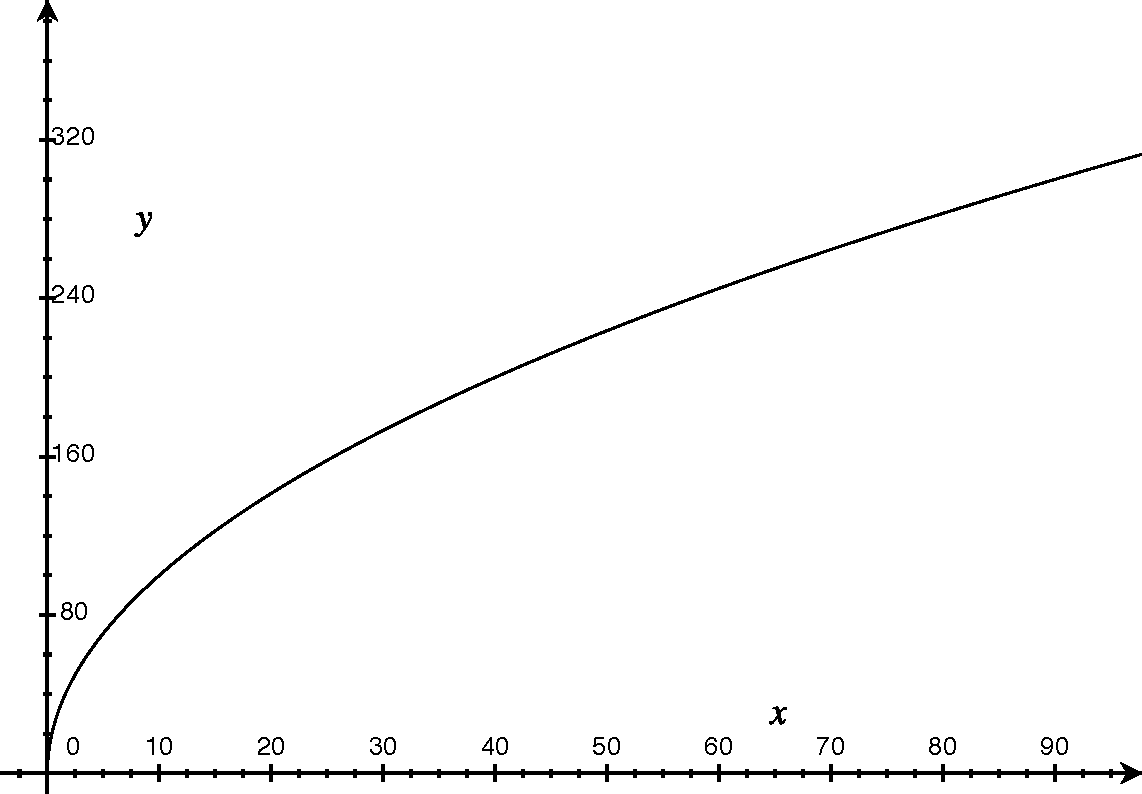
\includegraphics[width=0.6\linewidth]{./img/decutil}
\caption{Declining Marginal Utility of Money}
\label{fig:a Declining Marginal Utility of Money}
\end{figure}
\noindent You should read the $x$-axis there are measuring possible incomes in thousands of dollars per year, and the $y$-axis as measuring utility. The curve there is $y = x^{\frac{1}{2}}$. That isn't necessarily a plausible account of how much utility each income might give you, but it's close enough for our purposes. Note that although more income gives you more utility, the amount of extra utility you get from each extra bit of income goes down as you get more income. More precisely, the slope of the income-utility graph keeps getting shallower and shallower as your income/utility rises. (More precisely yet, a little calculus shows that the slope of the graph at any point is $\frac{1}{2y}$, which is obviously always positive, but gets less and less as your income/utility gets higher and higher.)

Now as you can see, that curve is rather steeping curving down. But it is common to think that in real life, the marginal utility of money diminishes even more quickly than that. Some economists think that the utility of a certain level of wealth is not best measured by the square root of that wealth level, but by the logarithm of it. On this way of thinking, multiplying your wealth by a common factor always has the same difference on your utility, whether that is taking your wealth from \$10,000 to \$100,000, or from \$1,000,000 to \$10,000,000. And some economists think that we can be satiated; that is, we can reach a point where extra material resources make no difference to utility at all. This is controversial; what is not controversial is the thesis that money has a declining marginal utility.

The fact that there is a declining marginal utility of money explains certain features of economic life. We'll look at models of two simple economic decisions, buying insurance and diversifying an investment portfolio. We'll then use what we said about diversified investments to explain some features of the actual insurance markets that we find.

\section{Insurance}
Imagine the utility an agent gets from an income of $x$ dollars is $x^{\frac{1}{2}}$. And imagine that right now their income is \$90,000. But there is a 5\% chance that something catastrophic will happen, and their income will be just \$14,400. So their expected income is $0.95 \times 90,000 + 0.05 \times 14,400 = 86220$. But their expected utility is just $0.95 \times 300 + 0.05 \times 120 = 291$, or the utility they would have with an income of \$84,861.

Now imagine this person is offered insurance against the catastrophic scenario. They can pay, say, \$4,736, and the insurance company will restore the \$75,600 that they will lose if the catastrophic event takes place. Their income is now sure to be \$85,264 (after the insurance is taken out), so they have a utility of 292. That's higher than what their utility was, so this is a good deal for them.

But note that it might also be a good deal for the insurance company. They receive in premiums \$4,736. And they have a 5\% chance of paying out \$75,600. So the expected outlay, in dollars, for them, is \$3,780. So they turn an expected profit on the deal. If they repeat this deal often enough, the probability that they will make a profit goes very close to 1.

The point of the example is that people are trying to maximise expected utility, while insurance companies are trying to maximise expected profits. Since there are cases where lowering your expected income can raise your expected utility, there is a chance for a win-win trade. And this possibility, that expected income can go down while expected utility can go up, is explained in virtue of the fact that there is a declining marginal utility of money. 

\section{Diversification}
Imagine that an agent has a starting wealth of 1, and the utility the agent gets from wealth $x$ is $x^{\frac{1}{2}}$. (We won't specify $x$ what, but take this to be some kind of substantial unit.) The agent has an opportunity to make an investment that has a 50\% chance of success and a 50\% chance of failure. If the agent invests $y$ in the scheme, the returns $r$ will be
\begin{equation*}
r = \begin{cases}4y,& \text{if success} ,\\ 0,& \text{if failure} .\end{cases}
\end{equation*}
The expected profit, in money, is $y$. That's because there is a 50\% chance of the profit being $3y$, and a 50\% chance of it being $-y$. But in utility, the expected return of investing 1 unit is 0. The agent has a 50\% chance of ending with a wealth of 4, i.e. a utility of 2, and a 50\% chance of ending with a wealth of 0, i.e. a utility of 0.

So making the investment doesn't seem like a good idea. But now imagine that the agent could, instead of putting all their money into this one venture, split the investment between two ventures that (a) have the same probability of returns as this one, and (b) their success of failure is probabilistically independent. So the agent invests $\frac{1}{2}$ in each deal. The agent's return will be
\begin{equation*}
r = \begin{cases}4,& \text{if both succeed} ,\\ 2,& \text{if one succeeds and the other fails},\\ 0,& \text{if both fail} .\end{cases}
\end{equation*}
The probability that both will succeed is $\frac{1}{4}$. The probability that one will succeed and the other fail is $\frac{1}{2}$. (Exercise: why is this number greater?) The probability that both will fail is $\frac{1}{4}$. So the agent's expected profit, in wealth, is 1. That is, it is $4 \times \frac{1}{4} + 2 \times \frac{1}{2} + 0 \times \frac{1}{4}$, i.e. 2, minus the 1 that is invested, so it is 2 minus 1, i.e. 1. So it's the same as before. Indeed, the expected profit on each investment is $\frac{1}{2}$. And the expected profits on a pair of investments is just the sum of the expected profits on each of the investments.

But the expected utility of the `portfolio' of two investments is considerably better than other portfolios with the same expected profit. One such portfolio is investing all of the starting wealth in one 50/50 scheme. The expected utility of the portfolio is $4^{\frac{1}{2}} \times \frac{1}{4} + 2^{\frac{1}{2}} \times \frac{1}{2} + 0 \times \frac{1}{4}$, which is about 1.21. So it's a much more valuable portfolio to the agent than the portfolio which had just a single investment. Indeed, the diversified investment is worth making, while the single investment was not worth making.

This is the general reason why it is good to have a diversified portfolio of investments. It isn't because the expected profits, measured in dollars, are higher this way. Indeed, diversification couldn't possibly produce a higher expected profit. That's because the expected profit of a portfolio is just the sum of the expected profits of each investment in the portfolio. What diversification can do is increase the expected utility of that return. Very roughly, the way it does this is by decreasing the probability of the worst case scenarios, and of the best case scenarios. Because the worst case scenario is more relevant to the expected utility calculation than the best case scenario, because in general it will be further from the median outcome, the effect is to increase the expected utility overall.

One way of seeing how important diversification is is to consider what happens if the agent again makes two investments like this, but the two investments are probabilistically linked. So if one investment succeeds, the other has an 80\% chance of success. Now the probability that both will succeed is 0.4, the probability that both will fail is 0.4, and the probability that one will succeed and the other fail is 0.2. The expected profit of the investments is still 1. (Each investment still has an expected profit of $\frac{1}{2}$, and expected profits are additive.) But the expected utility of the portfolio is just $4^{\frac{1}{2}} \times 0.4 + 2^{\frac{1}{2}} \times 0.2 + 0 \times 0.4$, which is about 1.08. The return on investment, in utility terms, has dropped by more than half.

The lesson is that for agents with declining marginal utilities for money, a diversified portfolio of investments can be more valuable to them than any member of the portfolio on its own could be. But this fact turns on the investments being probabilistically separated from one another.

\section{Selling Insurance}
In the toy example about insurance, we assumed that the marginal utility of money for the insurance company was flat. That isn't really true. The insurance company is owned by people, and the utility of return to those people is diminishing as the returns get higher. There is also the complication that the insurance company faces very different kinds of returns when it is above and below the solvency line.

Nevertheless, the assumption that the marginal utility of money is constant for the insurance company is constant is a useful fiction. And the reason that it is a useful fiction is that if the insurance company is well enough run, then the assumption is close to being true. By `well enough run', I simply mean that their insurance portfolio is highly diversified.

We won't even try to prove this here, but there are various results in probability theory that suggest that as long as there are a lot of different, and probabilistically independent, investments in a portfolio, then with a very high probability, the actual returns will be close to the expected returns. In particular, if the expected returns are positive, and the portfolio is large and diverse enough, then with a very high probability the actual returns will be positive. So, at least in optimal cases, it isn't a terrible simplification to treat the insurance company as if it was sure that it would actually get its expected profits. And if that's the case, the changing marginal utility of money is simply indifferent.

The mathematical results that are relevant here are what are sometimes called the ``Law of Large Numbers''. The law says that if you sample independent and identically distributed random variables repeatedly, then for any positive number $e$, the probability that the average output is within $e$ of the expected output goes to 1 as the number of samples goes to infinity. The approach can be quite quick in some cases. The following table lists the probability that the number of heads on $n$ flips of a random coin will be (strictly) between $0.4n$ and $0.6n$ for various values of $n$.

\starttab{c c}
\textbf{Number of flips} & \textbf{Probabiilty of between} $\mathbf{0.4n}$ \textbf{and} $\mathbf{0.6n}$ \textbf{heads} \\ 
1 & 0 \\
10 & 0.246 \\
20 & 0.497 \\
50 & 0.797 \\
100 & 0.943 \\
200 & 0.994 \\
500 & $>$ 0.99
\stoptab This depends crucially on independence. If the coin flips were all perfectly dependent, then the probabilities would not converge at all.

Note we've made two large assumptions about insurance companies. One is that the insurance company is large, the other is that it is diversified. Arguably both of these assumptions are true of most real-world insurance companies. There tend to be very few insurance companies in most economies. More importantly, those companies tend to be fairly diversified. You can see this in a couple of different features of modern insurance companies. 

One is that they work across multiple sectors. Most car insurance companies will also offer home insurance. Compare this to other industries. It isn't common for car sales agents to also be house sales agents. And it isn't common for car builders to also be house builders. The insurance industry tends to be special here. And that's because it's very attractive for the insurance companies to have somewhat independent business wings, such as car insurance and house insurance.

Another is that the products that are offered tend to be insurance on events that are somewhat probabilistically independent. If I get in a car accident, this barely makes a difference to the probability that you'll be in a car accident. So offering car insurance is an attractive line of business. Other areas of life are a little trickier to insure. If I lose my home to a hurricane, that does increase, perhaps substantially, the probability of you losing your house to a hurricane. That's because the probability of their being a hurricane, conditional on my losing my house to a hurricane, is 1. And conditional on their being a hurricane, the probability of you losing your house to a hurricane rises substantially. So offering hurricane insurance isn't as attractive a line of business as car insurance. Finally, if I lose my home to an invading army, the probability that the same will happen to you is very high indeed. In part for that reason, very few companies ever offer `invasion insurance'.

A lot of the financial crisis in the late 2000s was related to a similar problem. A lot of the financial institutions that failed were selling, either explicitly or effectively, mortgage insurance. That is, they were insuring various banks against the possibility of default. One problem with this is that mortgage defaults are not probabilistically independent. If I default on my mortgage, that could be because I lost my job, or it could be because my house price collapsed and I have no interest in sustaining my mortgage. Either way, the probability that you will also default goes up. (It goes up dramatically if I defaulted for the second reason.) What may have been sensible insurance policies to write on their own turned into massive losses because the insurers underestimated the probability of having to pay out on many policies all at once.

\chapter{Dutch Book Arguments}
\section{Probabilism}

So far we've been assuming that agents should have credence functions that look like probability functions. That is, we've been assuming that if $Cr$ is the function from propositions to an agent's confidence in that proposition, then $Cr$ is a probability function. In fact, we've often made that assumption completely implicitly, by just talking about the subjective probability of a proposition or state. But why should we believe that credences, or confidences, are probabilities?

One reason to believe this is that it seems to be obviously the right thing to believe in simple cases like drawing a marble from an urn with a known composition. If you know the proportion of marbles in the urn that are red, then your credence that the next marble to be drawn will be red should just equal that proportion. And since proportion functions just are probability functions, it follows in these simple cases that credences should be probabilities.

But the simple case is altogether too simple. Indeed, thinking about this case might make one think that probabilism is intuitively false. Many of the things we do not know are nothing like the draw of a marble from an urn. Think about how confident you are in any of the following propositions, or their negations.

\begin{enumerate*}
\item Google will be profitable in 100 years time.
\item The United States and Canada will fight at least one war in the next 500 years.
\item Jack the Ripper was a member of the aristocracy.
\item There are at least two gods.
\end{enumerate*}
Thinking about those examples suggests there is a distinction between economists (such as Frank Knight and John Maynard Keynes) called \textbf{risk} and \textbf{uncertainty}. A risky proposition, in this terminology, is one whose truth value we don't know, but for which there is a very good reason to assign a particular probability to it. That might be because we know its objective chance, or because it is part of a sequence with a known ratio of successes to failures. Other unknown propositions are uncertain propositions. This can come in degrees. It is only moderately uncertain how long each of you will live; actuarial tables plus knowing a bit about your social and medical background would suffice to give a pretty decent probability distribution over the range of possible life extents. On the other hand, it is completely uncertain how long the United States will live; it's hard to know what could remotely justify a particular probability in the proposition that the United States will cease to exist between 600 and 700 years from now.

For many highly uncertain propositions, it seems reasonable to have very little confidence in both the proposition and its negation. This does not mean having a credence close to one half. We can't, logically, have credences close to one-half in each of the following propositions.

\begin{itemize*}
\item The United States will cease to exist between 500 and 600 years from now.
\item The United States will cease to exist between 600 and 700 years from now.
\item The United States will cease to exist between 700 and 800 years from now.
\item The United States will cease to exist between 800 and 900 years from now.
\end{itemize*}
Yet each of these seems very uncertain. A widespread, if rarely popular, response to these cases has been to say that there are propositions in which a credence close to 0 in both $p$ and $\neg p$ is appropriate. What can probabilists say to such claims.

\section{Dutch Book Arguments}
One common response is to argue that anything other than probabilism leads to a certain kind of catastrophe. In particular, the agent whose credences are not probabilities will be led to a series of bets that lead to sure loss. I don't know how such a set of bets acquired this name, but they are now referred to as a \textit{Dutch Book}, and the activity of offering someone a series of bets that leads to a sure loss is known as \textit{making a book} against them.

Let's work through how this might work with a special case. Assume the agent in question is a \textit{miser}, by which we will mean that they value each dollar as much as the previous one. As we've seen, real people are not misers, and it is worthwhile to work through the argument without the assumption of miserliness. But we'll leave that activity as an exercise for the interested reader. (Hint: Replace the reference to dollars in what follows with tickets in a single lottery, and then argue that the agent will be a miser with respect to those tickets.)

Say that a $p$-bet is a bet that pays \$1 if $p$ is true, and nothing otherwise. The agent, if they are a miser, should value this bet at $Cr(p)$. If they don't have this valuation, then there is a good sense in which $Cr(p)$ is not really their credence in $p$; it isn't the mental state they have that drives action in the right way.

Now assume that the agent's credences do not generate a probability function. There are four ways that this could happen.

\begin{enumerate*}
\item It could be that for some $p$, $Cr(p) < 0$. In that case, they will regard a $p$-bet as a liability. So the bookmaker offers the agent a deal: the agent gives the bookmaker a $p$-bet, and the agent gives the bookmaker $Cr(p)$/2. Since this is a way of taking a liability away for less than half the cost of it, the agent likes the deal. But the bookmaker makes money whether $p$ is true or false.
\item It could be that for some $p$, $Cr(p) > 1$. In that case, the bookmaker sells the agent a $p$-bet for \$$(1 + Cr(p))/2$, and makes money whether $p$ is true or false.
\item It could be that for logically equivalent propositions $p$ and $q$, $Cr(p)$ and $Cr(q)$ are different. Assume that $Cr(p) > Cr(q)$. (If not, reverse what follows.) Then the bookmaker sells the agent a $p$-bet for \$$(2Cr(p) + Cr(q))/3$, and buys a $q$-bet from the agent for \$$(Cr(p) + 2Cr(q))/3$. The agent regards each of these trades as having positive value, so she makes each of them. The payoffs of the two bets are the same, so they cancel. But the bookmaker makes a profit of \$$(Cr(p) - Cr(q))/3$ on the trades, no matter what.
\item It could be that the agent has $Cr(p) + Cr(q) \neq Cr(p \vee q)$, for logically exclusive $p, q$. Assume the agent has $Cr(p \vee q) > Cr(p) + Cr(q)$. (The other case is left as an exercise.) Let $\epsilon$ be a small enough number that $Cr(p \vee q) > Cr(p) + Cr(q) + 3\epsilon$. The bookmaker sells the agent a $(p \vee q)$-bet for \$$Cr(p \vee q) - \epsilon$, and then buys a $p$-bet from the agent for \$$Cr(p) + \epsilon$, and buys a $q$-bet from the agent for \$$Cr(q) + \epsilon$. The agent regards each bet as having a positive value, so they make it. The payouts from the bets cancel. But the bookmaker has paid less for the bets they bought than they received for selling the $(p \vee q)$-bet, so they make a profit, no matter what.
\end{enumerate*}
The upshot is that any case where the agent's credences do not form a probability function is a case where a bookmaker can make a profit from the agent, no matter what.

\section{Objections}
Here are four objections to the argument from Dutch Books for probabilism. I don't mean these to exhaust the objections, but I do think these are particularly important objections.

\subsection{Wrong Kind of Failure}
The Dutch Book argument seems to show that agents who have non-probabilistic credences are doomed to make a certain kind of practical failure. They will, for certain, lose money. But what we started out wanting to show was that there was some kind of epistemological, or even logical, shortcoming to such agents. Indeed, in the literature it is common for probabilists to describe these agents as \textit{incoherent}. And being subject to a practical shortcoming does not seem to be a way of being incoherent.

\subsection{Betting Ex Ante and Ex Post}
Perhaps the fact that the agents are making a practical error could be a premise in an argument that they are making an epistemological error. If there were no explanation of why they are making a practical error, i.e., losing money, other than the epistemological error, then it might be a good inference from their practical failing to an epistemic shortcoming. Unfortunately, there are plenty of other explanations of why they might lose money. Perhaps they are not sufficiently sensitive to the existence of bookmakers.

The fact that the agent has credence $Cr(q)$ might mean that right now they value a $q$-bet and \$$Cr(q)$ the same. But it doesn't mean that they will willingly accept an offer to sell a $q$-bet for \$$Cr(q) + \epsilon$. After all, the fact that someone wants to buy something from you for more than you think it is worth is, in general, some evidence that you've undervalued the thing. Damon Runyon puts this point in the form of memorable advice.

\begin{quote}
One of these days in your travels, a guy is going to come up to you and show you a nice brand-new deck of cards on which the seal is not yet broken, and this guy is going to offer to bet you that he can make the Jack of Spades jump out of the deck and squirt cider in your ear. But, son, do not bet this man, for as sure as you are standing there, you are going to end up with an earful of cider.
\end{quote}

\subsection{See the Dutch Book Coming}
There is a distinct kind of practical mistake that the agent who buys a Dutch Book could be making. They might be failing to engage in appropriate \textbf{backwards induction} reasoning. We'll discuss this concept in greater detail in game theory, but it's a generally important idea. The thought is that when making choices in sequence, a rational agent should first think about what they'll do last. Then when making earlier choices, the agent should not look at the effect of the choice now, but about the ultimate result from heading down a particular path, assuming they will act rationally at later times.

Assume that the agent knows the plans of the bookmaker. And assume that the last trade the bookmaker offers is one that they will accept. (Backwards induction reasoning becomes single case reasoning at the last step, so that's a reasonable assumption.) Then the agent should not make the earlier trades. They know that making the earlier trades, even if they look good on their own, set them off down a path to ruin. And good dynamic traders do not set off on the path to ruin.

Is it fair to assume that the agent knows the plans of the bookmaker? I think it is. The bookmaker knows the plans of the bookmaker. And there isn't anything too surprising about the conclusion that if X knows something Y doesn't, then X can make money trading with Y. That doesn't show Y has incoherent credal attitudes. (It might show Y is foolish to trade with someone who knows more than they do, but this is leading back to the Runyon point mentioned above.)

Does the Dutch Book have to be dynamic? Couldn't the bookmaker offer these bets all at once? They could, but then the agent would surely decline them, for accepting them as a unit would amount to giving money away.

\subsection{Dutch Books and Decidability}
Assume for a moment that I have non-probabilistic credal states about whether the United States will cease to exist in approximately 600 years. Then a Dutch Book can be made against me. Great. But the construction of those books assumed that we could decide which bets won or lost, and pay those bets out. And that's not going to happen; I'm not going to be around to see whether the bets won or lost. 

And even if someone, an angel perhaps, could make me lose a few pennies by running such a book on me, I'd find out something amazing about the future of the United States. I'd be happy to lose a few pennies to find that out.

This is relevant because the main cases where philosophers have objected to probabilism have been cases where we don't have any good way to even find out whether the propositions are true. Assuming that we can decide the propositions sufficiently in order to work out who wins and loses bets on them seems to me to feels like an illegitimate assumption, relative to that background.

\subsection{Dutch Books Without Bookmakers}

David Christensen has developed what seems to me to be the best response to these objections. He thinks that we should just view the bookmaker as a metaphorical device. The problem is not that the agent in question will actually turn into a money pump, and hand over money to the bookmaker. Rather, what the thought experiment involving the bookmaker makes vivid is that the agent values the same thing in two different ways, depending on how the thing is presented. And that, says Christensen, is a kind of incoherence.

This is, I think, a really nice response to the objections. That the agent values the same thing in two different ways, depending on the presentation, does seem like a kind of incoherence, and not just a flaw in practical rationality. Reasoning this way doesn't assume that the agent fails to use backwards induction, or fails to heed Runyon's advice. That's because we don't look to how the agent does or would bet, but just at how they actually, currently, vaoue. And we don't have to worry about the bets being decided, because we aren't assuming there will even be bets.

But there is still a problem for the argument. It isn't clear that the agent really does value the same thing in two different ways. Let's step through a case slowly to see this. Assume that the agent has the following attitudes:

\begin{itemize*}
\item $Cr(p) = 0.3$
\item $Cr(q) = 0.4$
\item $Cr(p \vee q) = 0.8$
\end{itemize*}
And assume that $p, q$ are logically exclusive. Now Christensen wants to argue that the following two goods are the same, but the agent values them differently.

\begin{enumerate*}
\item A bundle consisting of a $p$-bet plus a $q$-bet.
\item A $(p \vee q)$-bet.
\end{enumerate*}
The argument that they are the same is pretty good I think, since the bundles have of necessity the same payoffs. But what's the argument that the agent values them the same. We know the following. The agent values the second bundle at 80 cents. And the agent values the parts of the first bundle at 30 cents and 40 cents, respectively. But what do we know about how they value the bundle?

If the value of the bundle is the value of its parts, then the agent values the bundle at 70 cents. And then they are guilty of valuing the same thing two ways. But that seems like a very quick attribution. It isn't true in general that we value bundles as just the sums of parts. I might value a pair of shoes highly, but have little use for either shoe on its own. Economists say that in this case the goods are \textit{complementary} goods. That just means that their value as a bundle is greater than the sum of their value alone.

The non-probabilist can avoid incoherence if they say that the $p$-bet and the $q$-bet are complementary goods. Perhaps there are arguments that this is not something that they should say. After all, it is a bit odd that bets that cannot pay off together could be viewed as complementary. But it does seem very hard to find a watertight argument from the existence of Dutch Books to constraints on credences.


\chapter{Newcomb's Problem}
\section{The Puzzle}
In front of you are two boxes, call them A and B. You call see that in box B there is \$1000, but you cannot see what is in box A. You have a choice, but not perhaps the one you were expecting. Your first option is to take just box A, whose contents you do not know. Your other option is to take both box A and box B, with the extra \$1000.

There is, as you may have guessed, a catch. A demon has predicted whether you will take just one box or take two boxes. The demon is very good at predicting these things -- in the past she has made many similar predictions and been right every time. If the demon predicts that you will take both boxes, then she's put nothing in box A. If the demon predicts you will take just one box, she has put \$1,000,000 in box A. So the table looks like this.

\starttab{l  c  c}
& \textbf{Predicts 1 box} & \textbf{Predicts 2 boxes} \\ 
\textbf{Take 1 box} & \$1,000,000 & \$0 \\ 
\textbf{Take 2 boxes} & \$1,001,000 & \$1,000
\stoptab There are interesting arguments for each of the two options here.

The argument for taking just one box is easy. The way the story has been set up, lots of people have taken this challenge before you. Those that have taken 1 box have walked away with a million dollars. Those that have taken both have walked away with a thousand dollars. You'd prefer to be in the first group to being in the second group, so you should take just one box.

The argument for taking both boxes is also easy. Either the demon has put the million in the opaque or she hasn't. If she has, you're better off taking both boxes. That way you'll get \$1,001,000 rather than \$1,000,000. If she has not, you're better off taking both boxes. That way you'll get \$1,000 rather than \$0. Either way, you're better off taking both boxes, so you should do that.

Both arguments seem quite strong. The problem is that they lead to incompatible conclusions. So which is correct?

\section{Two Principles of Decision Theory}
The puzzle was first introduced to philosophers by Robert Nozick. And he suggested that the puzzle posed a challenge for the compatibility of two decision theoretic rules. These rules are

\begin{itemize*}
\item Never choose dominated options
\item Maximise expected utility
\end{itemize*}

Nozick argued that if we never chose dominated options, we would choose both boxes. The reason for this is clear enough. If the demon has put \$1,000,000 in the opaque box, then it is better to take both boxes, since getting \$1,001,000 is better than getting \$1,000,000. And if the demon put nothing in the opaque box, then your choices are \$1,000 if you take both boxes, or \$0 if you take just the empty box. Either way, you're better off taking both boxes. This is obviously just the standard argument for taking both boxes. But note that however plausible it is as an argument for taking both boxes, it is compelling as an argument that taking both boxes is a dominating option.

To see why Nozick thought that maximising expected utility leads to taking one box, we need to see how he is thinking of the expected utility formula. That formula takes as an input the probability of each state. Nozick's way of approaching things, which was the standard at the time, was to take the expected utility of an action $A$ to be given by the following sum

\begin{equation*}
Exp(U(A)) = Pr(S_1 | A)U(AS_1) + ... + Pr(S_n | A)U(AS_n)
\end{equation*}

Note in particular that we put into this formula the probability of each state \textit{given that A is chosen}. We don't take the unconditional probability of being in that state. These numbers can come quite dramatically apart.

In Newcomb's problem, it is actually quite hard to say what the probability of each state is. (The states here, of course, are just that there is either \$1,000,000 in the opaque box or that there is nothing in it.) But what's easy to say is the probability of each state given the choices you make. If you choose both boxes, the probability that there is nothing in the opaque box is very high, and the probability that there is \$1,000,000 in it is very low. Conversely, if you choose just the one box, the probability that there is \$1,000,000 in it is very high, and the probability that there is nothing in it is very low. Simplifying just a little, we'll say that this high probability is 1, and the low probabiilty is 0. When working out the utility calculations, it will be helpful to use the following abbreviations:

\begin{itemize*}
\item $B$ = Take \textbf{b}oth boxes;
\item $O$ = Take \textbf{o}ne box;
\item $M$ = \textbf{M}illion in opaque box;
\item $N$ = Nothing in opaque box.
\end{itemize*}
The expected utility of each choice then is

\begin{align*}
Exp(U(B)) \\
&= Pr(M | B)U(M \wedge B)\\
&+ Pr(N | B)U(N \wedge B) \\
 &= 0 \times 1,001,000 + 1 \times 1,000 \\
 &= 1,000 \\
Exp(U(O)) \\
&= Pr(M | O)U(M \wedge O)\\
&+ Pr(N | O)U(N \wedge O) \\
 &= 1 \times 1,000,000 + 0 \times 0 \\
 &= 1,000,000
 \end{align*}

I've assumed here that the marginal utility of money is constant, so we can measure utility by the size of the numerical prize. That's an idealisation, but hopefully a harmless enough one.

\section{Bringing Two Principles Together}
In earlier chapters we argued that the expected utility rule never led to a conflict with the dominance principle. But here it has led to a conflict. Something seems to have gone badly wrong.

The problem was that we've used two distinct definitions of expected utility in the two arguments. In the version we had used in previous chapters, we presupposed that the probability of the states was independent of the choices that were made. So we didn't talk about $Pr(S_1|A)$ or $Pr(S_1|B)$ or whatever. We simply talked about $Pr(S_1)$.

If you make that assumption, expected utility maximisation does indeed imply dominance. We won't rerun the entire proof here, but let's see how it works in this particular case. Let's say that the probability that there is \$1,000,000 in the opaque box is $x$. It won't matter at all what $x$ is. And assume that the expected utility of a choice $A$ is given by this formula, where we use the unconditional probability of states as inputs.

\begin{equation*}
Exp(U(A)) = Pr(S_1)U(AS_1) + ... + Pr(S_n | A)U(AS_n)
\end{equation*}

Applied to our particular case, that would give us the following calculations.

\begin{align*}
Exp(U(B)) \\
&= Pr(M)U(M \wedge B)\\
&+ Pr(N)U(N \wedge B) \\
&= x \times 1,001,000 + (1-x) \times 1,000 \\
 &= 1,000 + 1,000,000x \\
Exp(U(O)) \\
&= Pr(M)U(M \wedge O)\\
&+ Pr(N)U(N \wedge O)\\
 &= x \times 1,000,000 + (1-x) \times 0 \\
 &= 1,000,000x
 \end{align*}
 
And clearly the expected value of taking both boxes is 1,000 higher than the expected utility of taking just one box. So as long as we don't conditionalise on the act we are performing, there isn't a conflict between the dominance principle and expected utility maximisation.

While that does resolve the mathematical puzzle, it hardly resolves the underlying philosophical problem. Why, we might ask, shouldn't we conditionalise on the actions we are performing? In general, it's a bad idea to throw away information, and the choice that we're about to make is a piece of information. So we might think it should make a difference to the probabilities that we are using.

The best response to this argument, I think, is that it leads to the wrong results in Newcomb's problem, and related problems. But this is a somewhat controversial clam. After all, some people think that taking one box is the right result in Newcomb's problem. And as we saw above, if we conditionalise on our action, then the expected utility of taking one box is higher than the expected utility of taking both. So such theorists will not think that it gives the wrong answer at all. To address this worry, we need to look more closely back at Newcomb's original problem, and its variants.

\section{Well Meaning Friends}
The next few sections are going to involve looking at arguments that we should take both boxes in Newcomb's problem, or to rejecting arguments that we should only take one box.

The simplest argument is just a dramatisation of the dominance argument. But still, it is a way to see the force of that argument. Imagine that you have a friend who can see into the opaque box. Perhaps the box is clear from behind, and your friend is standing behind the box. Or perhaps your friend has super-powers that let them see into opaque boxes. If your friend was able to give you advice, and has your best interests at heart, they'll tell you to take both boxes. That's true whether or not there is a million dollars in the opaque box. Either way, they'll know that you're better off taking both boxes.

Of course, there are lots of cases where a friend with more knowledge than you and your interests at heart will give you advice that is different to what you might intuitively think is correct. Imagine that I have just tossed a biased coin that has an 80\% chance of landing heads. The coin has landed, but neither of us can see how it has landed. I offer you a choice between a bet that pays \$1 if it landed heads, and a bet that pays \$1 if it landed tails. Since heads is more likely, it seems you should take the bet on heads. But if the coin has landed tails, then a well meaning and well informed friend will tell you that you should bet on tails.

But that case is somewhat different to the friend in Newcomb's problem. The point here is that you know what the friend will tell you. And plausibly, whenever you know what advice a friend will give you, you should follow that advice. Even in the coin-flip case, if you knew that your friend would tell you to bet on tails, it would be smart to bet on tails. After all, knowing that your friend would give you that advice would be equivalent to knowing that the coin landed tails. And if you knew the coin landed tails, then whatever arguments you could come up with concerning chances of landing tails would be irrelevant. It did land tails, so that's what you should bet on.

There is another way to dramatise the dominance argument. Imagine that after the boxes are opened, i.e. after you know which state you are in, you are given a chance to revise your choice if you pay \$500. If you take just one box, then whatever is in the opaque box, this will be a worthwhile switch to make. It will either take you from \$0 to \$500, or from \$1,000,000 to \$1,000,500. And once the box is open, there isn't even an intuition that you should worry about how the box got filled. So you should make the switch.

But it seems plausible in general that if right now you've got a chance to do X, and you know that if you don't do X now you'll certainly pay good money to do X later, and you know that when you do that you'll be acting perfectly rationally, then you should simply do X. After all, you'll get the same result whether you do X now or later, you'll simply not have to pay the `late fee' for taking X any later. More relevantly to our case, if you would switch to X once the facts were known, even if doing so required paying a fee, then it seems plausible that you should simply do X now. It doesn't seem that including the option of switching after the boxes are revealed changes anything about what you should do before the boxes are revealed, after all.

Ultimately, I'm not sure that either of the arguments I gave here, either the well meaning friend argument or the switching argument, are any more powerful than the dominance argument. Both of them are just ways of dramatising the dominance argument. And someone who thinks that you should take just one box is, by definition, someone who isn't moved by the dominance argument. So let's look at other arguments for taking both boxes.

\section{Real Life Newcomb Cases}
In the previous notes we ended up saying that there are two quite different ways to think about utility expectations. We can use the unconditional probability of each state, or, for each choice, we can use the probabilities of each state conditional on the choice the agent makes. That is, we can take the expected utility of a choice $A$ to be given by one or other of the following formulae.
\begin{align*}
Pr(S_1)U(S_1A) + ...  + Pr(S_n)U(S_nA) \\
Pr(S_1|A)U(S_1A) + ...  + Pr(S_n|A)U(S_nA)
\end{align*}

It would be nice to know which of these is the right formula, since the two formulae disagree about cases like Newcomb's problem. Since we have a case where they disagree, a simple methodology suggests itself. Figure out what we should do in Newcomb's problem, and then select the formula which agrees with the correct answer. But this method has two flaws.

First, intuitions about Newcomb's puzzle are themselves all over the place. If we try to adjust our theory to match our judgments in Newcomb's problem, then different people will have different theories.

Second, Newcomb's problem is itself quite fantastic. This is part of why different people have such divergent intuitions on the example. But it also might make us think that the problem is not particularly urgent. If the two equations only come apart in fantastic cases like this, perhaps we can ignore the puzzles.

So it would be useful to come up with more realistic examples where the two equations come apart. It turns out that what is driving the divergence between the equations is that there is a common cause of the world being in a certain state and you making the choice that you make. Any time there is something in the world that tracks your decision making processes, we'll have a Newcomb like problem.

For example, imagine that we are in a Prisoners' Dilemma situation where we know that the other prisoner uses very similar decision making procedures to what we use. Here is the table for a Prisoners' Dilemma.

\starttab{c c  c}
 & \textbf{Other} & \textbf{Other} \\
 & \textbf{Cooperates} & \textbf{Defects} \\ 
\textbf{You Cooperate} & (3,3) & (0, 5) \\
\textbf{You Defect} & (5, 0) & (1, 1)
\stoptab In this table the notation ($x$, $y$) means that you get $x$ utils and the other person gets $y$ utils. Remember that utils are meant to be an overall measure of what you value, so it includes your altruistic care for the other person.

Let's see why this resembles a Newcomb problem. Assume that conditional on your performing an action $A$, the probability that the other person will do the same action is 0.9. Then, if we are taking probabilities to be conditional on choices, the expected utility of the two choices is

\begin{align*}
Exp(U(Coop)) &= 0.9 \times 3 + 0.1 \times 0 \\
  &= 2.7 \\
 Exp(U(Defect)) &= 0.1 \times 5 + 0.9 \times 1 \\
  &= 1.4
 \end{align*}
So if we use probabilities conditional on choices, we end up with the result that you should cooperate. But note that cooperation is dominated by defection. If the other person defects, then your choice is to get 1 (by defecting) or 0 (by cooperating). You're better off cooperating. If the other person cooperates, then your choice is to get 5 (by defecting) or 0 (by cooperating). So whatever probability we give to the possible actions of the other person, provided we don't conditionalise on our choice, we'll end up deciding to defect.

Prisoners Dilemma cases are much less fantastic than Newcomb problems. Even Prisoners Dilemma cases where we have some confidence that the other party sufficiently resembles us that they will likely (not certainly) make the same choice as us are fairly realistic. So they are somewhat better than Newcomb's original problem for detecting intuitions. But the problem of divergent intuitions still remains. Many people are unsure about what the right thing to do in a Prisoners Dilemma problem is. 

So it is worth looking at some cases without that layer of complication. Real life cases are tricky to come by, but for a while some people suggested that the following might be a case. We've known for a long time that smoking causes various cancers. We've known for even longer than that that smoking is correlated with various cancers. For a while there was a hypothesis that smoking did not cause cancer, but was correlated with cancer because there was a common cause. Something, presumably genetic, caused people to (a) have a disposition to smoke, and (b) develop cancer. Crucially, this hypothesis went, smoking did not raise the risk of cancer; whether you got cancer or not was largely due to the genes that led to a desire for smoking.

We now know, by means of various tests, that this isn't true. (For one thing, the reduction in cancer rates among people who give up smoking is truly impressive, and hard to explain on the model that these cancers are all genetic.) But at least at some point in history it was a not entirely crazy hypothesis. Let's assume this hypothesis is actually true (contrary to fact). And let's assume that you (a) want to smoke, other things being equal, and (b) really don't want to get cancer. You don't know whether you have the desire for smoking/disposition to get cancer gene or not? What should you do?

Plausibly, you should smoke. You either have the gene or you don't. If you do, you'll probably get cancer, but you can either get cancer while smoking, or get cancer while not smoking, and since you enjoy smoking, you should smoke. If you don't, you won't get cancer whether you smoke or not, so you should indulge your preference for smoking.

It isn't just philosophers who think this way. At some points (after the smoking/cancer correlation was discovered but before the causal connection was established) various tobacco companies were trying very hard to get evidence for this `common cause' hypothesis. Presumably the reason they were doing this was because they thought that if it were true, it would be rational for people to smoke more, and hence people would smoke more.

But note that this presumption is true if and only if we use the `unconditional' version of expected utility theory. To see this, we'll use the following table for the various outcomes.
\starttab{r c  c}
 & \textbf{Get Cancer} & \textbf{Don't get Cancer} \\ 
\textbf{Smoke} & 1 & 6 \\
\textbf{Don't Smoke} & 0 & 5
\stoptab 
The assumption is that not getting cancer is worth 5 to you, while smoking is worth 1 to you. Now we know that smoking is evidence that you have the cancer gene, and this raises dramatically the chance of you getting cancer. So the (evidential) probability of getting cancer conditional on smoking is, we'll assume, 0.8, while the (evidential) probability of getting cancer conditional on not smoking is, we'll assume, 0.2. And remember this isn't because cancer causes smoking in our example, but rather that there is a common cause of the two. Still, this is enough to make the expected utilities work out as follows. 

\begin{align*}
Exp(U(Smoke)) &= 0.8 \times 1 + 0.2 \times 6 \\
  &= 2 \\
Exp(U(No Smoke)) &= 0.2 \times 0 + 0.8 \times 5 \\
  &= 4
 \end{align*}

And the recommendation is not to smoke, even though smoking dominates. This seems very odd. As it is sometimes put, the recommendation here seems to be a matter of managing the `news', not managing the outcome. What's bad about smoking is that if you smoke you get some evidence that something bad is going to happen to you. In particular, you get evidence that you have this cancer gene, and that's really bad news to get because dramatically raises the probability of getting cancer. But not smoking doesn't mean that you don't have the gene, it just means that you don't find out that you have the gene. Not smoking looks like a policy of denying yourself good outcomes because you don't want to get bad news. And this doesn't look rational.

So this case has convinced a lot of decision theorists that we shouldn't use conditional probabilities of states when working out the utility of various outcomes. Using conditional probabilities will be good if we want to learn the `news value' of some choices, but not if we want to learn how useful those choices will be to us.

\section{Tickle Defence}
Not everyone has been convinced by these `real-life' examples. The counter-argument is that in any realistic case, the gene that leads to smoking has to work by changing our dispositions. So there isn't just a direct causal connection between some genetic material and smoking. Rather, the gene causes a desire to smoke, and the desire to smoke cause the smoking. As it is sometimes put, between the gene and the smoking there has to be something mental, a `tickle' that leads to the smoking.

Now this is important because we might think that rational agents know their own mental states. Let's assume that for now. So if an agent has the smoking desire they know it, perhaps because this desire has a distinctive phenomenology, a tickle of sorts. And if the agent knows this, then they won't get any extra evidence that they have a desire to smoke from their actual smoking. So the probability of getting cancer given smoking is not higher than the probability of getting cancer given not smoking.

In the case we have in mind, the bad news is probably already here. Once the agent realises that their values are given by the table above, they've already got the bad news. Someone who didn't have the gene wouldn't value smoking more than not smoking. Once the person conditionalises on the fact that that is their value table, the evidence that they actually smoke is no more evidence. Either way, they are (say) 80\% likely to get cancer. So the calculations are really something like this:

 \begin{align*}
Exp(U(Smoke)) &= 0.8 \times 1 + 0.2 \times 6 \\
  &= 2 \\
 Exp(U(No Smoke)) &= 0.8 \times 0 + 0.2 \times 5 \\
  &= 1
\end{align*}
And we get the correct answer that in this situation we should smoke. So this isn't a case where the two different equations we've used give different answers. And hence it isn't a reason for using unconditional probabilities rather than conditional probabilities.

There are two common responses to this argument. The first is that it isn't clear that there is always a `tickle'. The second is that it isn't a requirement of rationality that we know what tickles we have. Let's look at these in turn.

First, it was crucial to this defence that the gene (or whatever) that causes both smoking and cancer causes smoking by causing some particular mental state first. But this isn't a necessary feature of the story. It might be that, say, everyone has the `tickle' that goes along with wanting to smoke. (Perhaps this desire has some evolutionary advantage. Or, more likely, it might be a result of something that genuinely had evolutionary advantage.) Perhaps what the gene does is to affect how much willpower we have, and hence how likely we are to overcome the desire. 

Second, it was also crucial to the defence that it is a requirement of rationality that people know what `tickles' they have. If this isn't supposed, we can just imagine that our agent is a rational person who is ignorant of their own desires. But this supposition is quite strong. It is generally not a requirement of rationality that we know things about the external world. Some things are just hidden from us, and it isn't a requirement of rationality that we be able to see what is hidden. Similarly, it seems at least possible that some things in our own mind should be hidden. Whether or not you believe in things like subconscious desires, the possibility of them doesn't seem to systematically undermine human rationality.

Note that these two responses dovetail nicely. If we think that the gene works not by producing individual desires, but by modifying quite general standing dispositions like how much willpower we have, it is even more plausible to think that this is not something a rational person will always know about. It is a little odd to think of a person who desires to smoke but doesn't realise that they desire to smoke. It isn't anywhere near as odd to think about a person who has very little willpower but, perhaps because their willpower is rarely tested, doesn't realise that they have low willpower. Unless they are systematically ignoring evidence that they lack willpower, they aren't being clearly irrational.

So it seems there are possible, somewhat realistic, cases where one choice is evidence, to a rational agent, that something bad is likely to happen, even though the choice does not bring about the bad outcome. In such a case using conditional probabilities will lead to avoiding the bad news, rather than producing the best outcomes. And that seems to be irrational.

\chapter{Causal Decision Theory}
\section{Causal and Evidential Decision Theory}
In the last chapter we looked at two ways of thinking about the expected utility of an action $A$. These are \begin{align*}
Pr(S_1)U(S_1A) + ...  + Pr(S_n)U(S_nA) \\
Pr(S_1|A)U(S_1A) + ...  + Pr(S_n|A)U(S_nA)
\end{align*}

\noindent It will be convenient to have names for these two approaches. So let's say that the first of these, which uses unconditional probabilities, is \textbf{causal expected value}, and the second of these, which uses conditional probabilities is the \textbf{evidential expected value}. The reason for the names should be clear enough. The causal expected value measures what you can expect to bring about by your action. The evidential expected value measures what kind of result your action is evidence that you'll get.

\textbf{Causal Decision Theory} then is the theory that rational agents aim to maximise causal expected utility.

\textbf{Evidential Decision Theory} is the theory that rational agents aim to maximise evidential expected utility.

In the last chapter we looked at reasons why we should be causal decision theorists rather than evidential decision theorists. We'll close out this section by looking at various puzzles for causal decision theory, and then looking at one reason why we might want some kind of hybrid approach.

\section{Right and Wrong Tabulations}
If we use the causal approach, it is very important how we divide up the states. We can see this by thinking again about an example from Jim Joyce that we discussed a while ago.

\begin{quotation}
Suupose you have just parked in a seedy neighborhood when a man approaches and offers to ``protect'' your car from harm for \$10. You recognize this as extortion and have heard that people who refuse ``protection'' invariably return to find their windshields smashed. Those who pay find their cars intact. You cannot park anywhere else because you are late for an important meeting. It costs \$400 to replace a windshield. Should you buy ``protection''? Dominance says that you should not. Since you would rather have the extra \$10 both in the even that your windshield is smashed and in the event that it is not, Dominance tells you not to pay. (Joyce, \textit{The Foundations of Causal Decision Theory}, pp 115-6.)
\end{quotation}

\noindent If we set this up as a table, we get the following possible states and outcomes.

\starttab{r c  c}
& \textbf{Broken Windshield} & \textbf{Unbroken Windshield} \\
\textbf{Pay extortion} & -\$410 & -\$10 \\
\textbf{Don't pay} & -\$400 & 0
\stoptab Now if you look at the causal expected value of each action, the expected value of not paying will be higher. And this will be so whatever probabilities you assign to broken windshield and unbroken windshield. Say that the probability of the first is $x$ and of the second is $1-x$. Then we'll have the following (assuming dollars equal utils)
\begin{align*}
Exp(U(\text{Pay extortion})) &= -410x -10(1-x) \\
 &= -400x - 10 \\
Exp(U(\text{Don't pay}) &= -400x -0(1-x) \\
 &= -400x
\end{align*}

Whatever $x$ is, the causal expected value of not paying is higher by 10. That's obviously a bad result. Is it a problem for causal decision theory though? No. As the name `causal' suggests, it is crucial to causal decision theory that we separate out what we have causal power over from what we don't have causal power over. The states of the world represent what we can't control. If something can be causally affected by our actions, it can't be a background state.

So this is a complication in applying causal decision theory. Note that it is not a problem for evidential decision theory. We can even use the very table that we have there. Let's assume that the probability of broken windshield given paying is 0, and the probability of unbroken windshield given paying is 0. Then the expected utilities will work out as follows \begin{align*}
Exp(U(\text{Pay extortion})) &= -410 \times 0 -10 \times 1 \\
 &=  -10 \\
Exp(U(\text{Don't pay}) &= -400 \times 1 - 10 \times 0 \\
 &= -400
\end{align*} So we get the right result that we should pay up. It is a nice feature of evidential decision theory that we don't have to be so careful about what states are and aren't under our control. Of course, if the only reason we don't have to worry about what is and isn't under our control is that the theory systematically ignores such facts, even though they are intuitively relevant to decision theory, this isn't perhaps the best advertisement for evidential decision theory.

\section{Why Ain'Cha Rich}
You might think that the following argument for taking one-box is compelling.

\begin{enumerate*}
\item Most people who take one box end up rich, and most people who take two boxes don't.
\item It is better, at least in the context of this puzzle, to end up rich than not.
\item So you should do what the people who end up rich do.
\item So you should take one box.
\end{enumerate*}

\noindent The problem is that this argument over-generates. The same argument implies that you should take just one box in the case where the demon makes the prediction, and then tells you what it is, before you choose. Call this case \textit{Transparent Newcomb's Problem}. Evidential decision theory says that you should take both boxes in it, just like causal decision theory says. But the kind of reasoning we just laid out says you should take one box in both the regular and transparent version of Newcomb's Problem. So the reasoning must be flawed.

\section{Dilemmas}
Consider the following story, told by Allan Gibbard and William Harper in their paper setting out causal decision theory. \begin{quote}
Consider the story of the man who met Death in Damascus. Death looked surprised, but then recovered his ghastly composure and said, 
`I {\sc am coming for you tomorrow}'. The terrified man that night bought a camel and rode to Aleppo. The next day, Death knocked on the door of the room where he was hiding, and said `I {\sc have come for you}'. 

`But I thought you would be looking for me in Damascus', said the man.
 
`{\sc Not at all}', said Death `{\sc that is why I was surprised to see you yesterday. I knew that today I was to find you in Aleppo}'. 

Now suppose the man knows the following. Death works from an appointment book which states time and place; a person dies if and only if the book correctly states in what city he will be at the stated time. The book is made up weeks in advance on the basis of highly reliable predictions. An appointment on the next day has been inscribed for him. Suppose, on this basis, the man would take his being in Damascus the next day as strong evidence that his appointment with Death is in Damascus, and would take his being in Aleppo the next day as strong evidence that his appointment is in Aleppo...
 
If... he decides to go to Aleppo, he then has strong grounds for expecting that Aleppo is where Death already expects him to be, and hence it is rational for him to prefer staying in Damascus. Similarly, deciding to stay in Damascus would give him strong grounds for thinking that he ought to go to Aleppo.
\end{quote}
In cases like this, the agent is in a real dilemma. Whatever he does, it seems that it will be the wrong thing. If he goes to Aleppo, then Death will probably be there. And if he stays in Damascus, then Death will probably be there as well. So it seems like he is stuck.

Of course in one sense, there is clearly a right thing to do, namely go wherever Death isn't. But that isn't the sense of right decision we're typically using in decision theory. Is there something that he can do that maximises expected utility. In a sense the answer is ``No''. Whatever he does, doing that will be some evidence that Death is elsewhere. And what he should do is go wherever his evidence suggests Death isn't. This turns out to be impossible, so the agent is bound not to do the rational thing.

Is this a problem for causal decision theory? It is if you think that we should always have a rational option available to us. If you think that `rational' here is a kind of `ought', and you think `ought' implies `can', then you might think we have a problem, because in this case there's a sense in which the man can't do the right thing. (Though this is a bit unclear; in the actual story, there's a perfectly good sense in which he could have stayed in Aleppo, and the right thing to do, given his evidence, would have been to stay in Aleppo. So in one sense he could have done the right thing.) But both the premises of the little argument here are somewhat contentious. It isn't clear that we should say you ought, in any sense, maximise expected utility. And the principle that ought implies can is rather controversial. So perhaps this isn't a clear counterexample to causal decision theory.

The response that Gibbard and Harper give to this puzzle is that it is just a dil\-emma. Whatever the man plays, he'll regret it. That's one way of rejecting the ought implies can premise. Not everyone is convinced by that move. Reed Richter argued that this was the wrong thing to say about \textit{asymmetric} versions of the Death in Damascus case. Imagine that getting to Aleppo will cost a huge amount of money, and be incredibly painful. Then the table might look something like this:

\starttab{r c c}
%This is called AsymmetricDeathinDamascus
%It is Matching Pennies with Asymmetries
\gamelab{AsymmetricDeathinDamascus} & \textbf{Damascus} & \textbf{Aleppo} \\
\textbf{Damascus} & 1, -1 & -1, 0.5 \\
\textbf{Aleppo} & -1, 1 & 1, -1.5 \\
\fintab Again, whatever the man does, he will regret it, just like in the original Death in Damascus example. But it seems wrong to treat the two options available to the man symmetrically. After all, going to Aleppo is much worse for him. If forced to choose, Richter argued, he should stay in Damascus. Let's look at that case again after looking at a third kind of solution to the puzzle.

\section{Ratificationism}

Some people don't like Causal Decision Theory because it trucks in metaphysical notions like causation and counterfactuals. Richard Jeffrey was worried that Causal Decision Theory was too metaphysical, but he agreed that we should take both boxes in Newcomb's Problem. So he promoted a \textit{Ratificationist} version of Evidential Decision Theory.

The idea behind ratificationism is that only \textit{ratifiable} decisions are rationally allowed. A decision is ratifiable if it maximises expected utility conditional on that decision being taken. We can add a ratifiability clause to Evidential Decision Theory, as Jeffrey does, or to Causal Decision Theory, as (in effect) Frank Arntzenius has recently suggested. 

If we add a ratifiability clause to Evidential Decision Theory, we get the result that rational agents should take both boxes. That's because only it is ratifiable. We computed earlier the expected utility of each choice according to Evidential Decision Theory, and concluded that the utility of taking just one box was higher. But now look what happens if we conditionalise on the hypothesis that we'll take just one box. (For simplicity, we'll again assume \$1 is worth 1 util.) It is easy enough to see that taking both boxes is better.

\begin{align*}
\Pr(\text{Million in opaque box} | \text{Take one box}) &= 0.99 \text{therefore} \\
V(\text{Take one box} | \text{Take one box}) &= 0.99 \times 1,000,000 + 0.01 \times 0 \\
&= 990,000 \\
V(\text{Take both boxes} | \text{Take one box}) &= 0.99 \times 1,001,000 + 0.01 \times 1,000 \\
&= 991,000 
\end{align*} But there is something very odd about this way of putting things. It requires thinking about the expected value of an action conditional on something that entails the action is not taken. In Newcomb's Problem we can sort of make sense of this; we use the conditional assumption that we're taking one box to seed the probability of the demon doing certain actions, then we run the calculations from there. But I don't see any reason to think that we should, in general, be able to make sense of this notion.

A better approach, I think, is to mix ratificationism with Causal Decision Theory.  This lets us solve what's otherwise a hard problem for Causal Decision Theory. Note that when we argued that Causal Decision Theory implies you should take both boxes, we argued somewhat indirectly. We argued that Causal Decision Theory validated dominance reasoning in Newcomb's Problem, and dominance reasoning implied taking both boxes. We didn't do what you'd expect someone using Causal Decision Theory to do, of finding the values for the two choices and comparing them. And that leads to some problems. Imagine the following situation. You are offered the choice between getting \$2,000 for certain, and playing the game with the demon and the boxes. You might feel that you should take the money, but Causal Decision Theory on its own has a hard time generating that verdict.

Adding ratification makes the problem easier. Let's assume the demon is very very accurate; given that the player is choosing $\varphi$, the probability that the demon will predict $\varphi$ is 0.9999. Now let's work through the values of taking each of the options. (Let $p_i$ is the proposition that the demon predicts that $i$ boxes will be taken. We'll use $T_i$ as shorthand for \textit{Take i boxes}. And we'll assume, again that a dollar is worth a util.)
\begin{align*}
U(T_1 | T_1) &= \Pr(T_1 \boxright p_1 | T_1)U(T_1 \wedge p_1) + \Pr(T_1 \boxright p_2 | T_1)U(T_1 \wedge p_2) \\
&= 0.9999 \times 1,000,000 + 0.0001 \times 0 \\
&= 999,900 \\
U(T_2 | T_1) &= \Pr(T_2 \boxright p_1 | T_1)U(T_2 \wedge p_1) + \Pr(T_2 \boxright p_2 | T_1)U(T_2 \wedge p_2) \\
&= 0.9999 \times 1,001,000 + 0.0001 \times 1,000 \\
&= 1,001,900 \\
U(T_1 | T_2) &= \Pr(T_1 \boxright p_1 | T_2)U(T_1 \wedge p_1) + \Pr(T_1 \boxright p_2 | T_2)U(T_1 \wedge p_2) \\
&= 0.0001 \times 1,000,000 + 0.9999 \times 0 \\
&= 100 \\
U(T_2 | T_2) &= \Pr(T_2 \boxright p_1 | T_2)U(T_2 \wedge p_1) + \Pr(T_2 \boxright p_2 | T_2)U(T_2 \wedge p_2) \\
&= 0.0001 \times 1,001,000 + 0.9999 \times 1,000 \\
&= 1,100	
\end{align*} The important thing to note about this calculation is that $\Pr(T_2 \boxright p_1 | T_1)$ is very high, 0.9999 in our version of the game. What this says is that once we've assumed $T_1$, then the counterfactual $T_2 \boxright p_1$ is very very probable. That is, given that we're taking 1 box, it is very probable that if we had taken 2 boxes, there would still have been money in the opaque box. But that's just what Newcomb's problem suggests.

Note that neither $T_1$ nor $T_2$ is ratifiable. Given $T_1$, the player would be better with $T_2$. (The expected value of taking both boxes would be 1,001,900, as compared to an expected value of 999,900 for taking one box.) And given $T_2$, the player would be better with simply taking the \$2,000 and not playing, since the expected payout of $T_2$ is a mere 1,100. But taking \$2,000 is ratifiable. Given that the player is doing this, no other option is better. After all, if they are the kind of player who is moved by the reasoning that leads to taking the \$2,000, then they are almost certainly two boxers, and so probably the opaque box would be empty. So the only ratifiable decision is to take \$2,000. This ratificationist argument is, I think, intuitively plausible.

\section{Weak Newcomb Problems}
Imagine a small change to the original Newcomb problem. Instead of there being \$1000 in the clear box, there is \$800,000. Still, evidential decision theory recommends taking one box. The evidential expected value of taking both boxes is now roughly \$800,000, while the evidential expected value of taking just the one box is \$1,000,000. Causal decision theory recommends taking both boxes, as before.

So neither theory changes its recommendations when we increase the amount in the clear box. But I think many people find the case for taking just the one box to be less compelling in this variant. Does that suggest we need a third theory, other than just causal or evidential decision theory?

It turns out that we can come up with hybrid theories that recommend taking one box in the original case, but two boxes in the original case. Remember that in principle anything can have a probability, including theories of decision. So let's pretend that given the (philosophical) evidence on the table, the probability of causal decision theory is, say, 0.8, while the probability of evidential decision theory is 0.2. (I'm not saying these numbers are right, this is just a possibility to float.) And let's say that we should do the thing that has the highest \textit{expected} expected utility, where we work out expected expected utilities by summing over the expectation of the action on different theories, times the probability of each theory. (Again, I'm not endorsing this, just floating it.)

Now in the original Newcomb problem, evidential decision theory says taking one boxes is \$999,000 better, while causal decision theory say staking both boxes is \$1,000 better. So the expected expected utility of taking one box rather than both boxes is $0.2 \times 999,000 - 0.8 \times 1,000$, which is 199,000. So taking one box is `better' by 199,000

In the modified Newcomb problem, evidential decision theory says taking one boxes is \$200,000 better, while causal decision theory says taking both boxes is \$800,000 better. So the expected expected utility of taking one box rather than both boxes is $0.2 \times 200,000 - 0.8 \times 800,000$, i.e., -600,000. So taking both boxes is `better' by 600,000.

If you think that changing the amount in the clear box can change your decision in Newcomb's problem, then possibly you want a hybrid theory, perhaps like the one floated here.


%\chapter{Realistic Newcomb Problems}
%\section{Real Life Newcomb Cases}
In the previous notes we ended up saying that there are two quite different ways to think about utility expectations. We can use the unconditional probability of each state, or, for each choice, we can use the probabilities of each state conditional on the choice the agent makes. That is, we can take the expected utility of a choice $A$ to be given by one or other of the following formulae.
\begin{align*}
Pr(S_1)U(S_1A) + ...  + Pr(S_n)U(S_nA) \\
Pr(S_1|A)U(S_1A) + ...  + Pr(S_n|A)U(S_nA)
\end{align*}

It would be nice to know which of these is the right formula, since the two formulae disagree about cases like Newcomb's problem. Since we have a case where they disagree, a simple methodology suggests itself. Figure out what we should do in Newcomb's problem, and then select the formula which agrees with the correct answer. But this method has two flaws.

First, intuitions about Newcomb's puzzle are themselves all over the place. If we try to adjust our theory to match our judgments in Newcomb's problem, then different people will have different theories.

Second, Newcomb's problem is itself quite fantastic. This is part of why different people have such divergent intuitions on the example. But it also might make us think that the problem is not particularly urgent. If the two equations only come apart in fantastic cases like this, perhaps we can ignore the puzzles.

So it would be useful to come up with more realistic examples where the two equations come apart. It turns out that what is driving the divergence between the equations is that there is a common cause of the world being in a certain state and you making the choice that you make. Any time there is something in the world that tracks your decision making processes, we'll have a Newcomb like problem.

For example, imagine that we are in a Prisoners' Dilemma situation where we know that the other prisoner uses very similar decision making procedures to what we use. Here is the table for a Prisoners' Dilemma.

\starttab{c || c  c}
 & Other & Other \\
 & Cooperates & Defects \\ \hline
You Cooperate & (3,3) & (0, 5) \\
You Defect & (5, 0) & (1, 1)
\stoptab In this table the notation ($x$, $y$) means that you get $x$ utils and the other person gets $y$ utils. Remember that utils are meant to be an overall measure of what you value, so it includes your altruistic care for the other person.

Let's see why this resembles a Newcomb problem. Assume that conditional on your performing an action $A$, the probability that the other person will do the same action is 0.9. Then, if we are taking probabilities to be conditional on choices, the expected utility of the two choices is

\begin{align*}
Exp(U(Coop)) &= 0.9 \times 3 + 0.1 \times 0 \\
  &= 2.7 \\
 Exp(U(Defect)) &= 0.1 \times 5 + 0.9 \times 1 \\
  &= 1.4
 \end{align*}
So if we use probabilities conditional on choices, we end up with the result that you should cooperate. But note that cooperation is dominated by defection. If the other person defects, then your choice is to get 1 (by defecting) or 0 (by cooperating). You're better off cooperating. If the other person cooperates, then your choice is to get 5 (by defecting) or 0 (by cooperating). So whatever probability we give to the possible actions of the other person, provided we don't conditionalise on our choice, we'll end up deciding to defect.

Prisoners Dilemma cases are much less fantastic than Newcomb problems. Even Prisoners Dilemma cases where we have some confidence that the other party sufficiently resembles us that they will likely (not certainly) make the same choice as us are fairly realistic. So they are somewhat better than Newcomb's original problem for detecting intuitions. But the problem of divergent intuitions still remains. Many people are unsure about what the right thing to do in a Prisoners Dilemma problem is. 

So it is worth looking at some cases without that layer of complication. Real life cases are tricky to come by, but for a while some people suggested that the following might be a case. We've known for a long time that smoking causes various cancers. We've known for even longer than that that smoking is correlated with various cancers. For a while there was a hypothesis that smoking did not cause cancer, but was correlated with cancer because there was a common cause. Something, presumably genetic, caused people to (a) have a disposition to smoke, and (b) develop cancer. Crucially, this hypothesis went, smoking did not raise the risk of cancer; whether you got cancer or not was largely due to the genes that led to a desire for smoking.

We now know, by means of various tests, that this isn't true. (For one thing, the reduction in cancer rates among people who give up smoking is truly impressive, and hard to explain on the model that these cancers are all genetic.) But at least at some point in history it was a not entirely crazy hypothesis. Let's assume this hypothesis is actually true (contrary to fact). And let's assume that you (a) want to smoke, other things being equal, and (b) really don't want to get cancer. You don't know whether you have the desire for smoking/disposition to get cancer gene or not? What should you do?

Plausibly, you should smoke. You either have the gene or you don't. If you do, you'll probably get cancer, but you can either get cancer while smoking, or get cancer while not smoking, and since you enjoy smoking, you should smoke. If you don't, you won't get cancer whether you smoke or not, so you should indulge your preference for smoking.

It isn't just philosophers who think this way. At some points (after the smoking/cancer correlation was discovered but before the causal connection was established) various tobacco companies were trying very hard to get evidence for this `common cause' hypothesis. Presumably the reason they were doing this was because they thought that if it were true, it would be rational for people to smoke more, and hence people would smoke more.

But note that this presumption is true if and only if we use the `unconditional' version of expected utility theory. To see this, we'll use the following table for the various outcomes.
\starttab{r || c  c}
 & Get Cancer & Don't get Cancer \\ \hline
Smoke & 1 & 6 \\
Don't Smoke & 0 & 5
\stoptab 
The assumption is that not getting cancer is worth 5 to you, while smoking is worth 1 to you. Now we know that smoking is evidence that you have the cancer gene, and this raises dramatically the chance of you getting cancer. So the (evidential) probability of getting cancer conditional on smoking is, we'll assume, 0.8, while the (evidential) probability of getting cancer conditional on not smoking is, we'll assume, 0.2. And remember this isn't because cancer causes smoking in our example, but rather that there is a common cause of the two. Still, this is enough to make the expected utilities work out as follows. 

\begin{align*}
Exp(U(Smoke)) &= 0.8 \times 1 + 0.2 \times 6 \\
  &= 2 \\
Exp(U(No Smoke)) &= 0.2 \times 0 + 0.8 \times 5 \\
  &= 4
 \end{align*}

And the recommendation is not to smoke, even though smoking dominates. This seems very odd. As it is sometimes put, the recommendation here seems to be a matter of managing the `news', not managing the outcome. What's bad about smoking is that if you smoke you get some evidence that something bad is going to happen to you. In particular, you get evidence that you have this cancer gene, and that's really bad news to get because dramatically raises the probability of getting cancer. But not smoking doesn't mean that you don't have the gene, it just means that you don't find out that you have the gene. Not smoking looks like a policy of denying yourself good outcomes because you don't want to get bad news. And this doesn't look rational.

So this case has convinced a lot of decision theorists that we shouldn't use conditional probabilities of states when working out the utility of various outcomes. Using conditional probabilities will be good if we want to learn the `news value' of some choices, but not if we want to learn how useful those choices will be to us.

\section{Tickle Defence}
Not everyone has been convinced by these `real-life' examples. The counter-argument is that in any realistic case, the gene that leads to smoking has to work by changing our dispositions. So there isn't just a direct causal connection between some genetic material and smoking. Rather, the gene causes a desire to smoke, and the desire to smoke cause the smoking. As it is sometimes put, between the gene and the smoking there has to be something mental, a `tickle' that leads to the smoking.

Now this is important because we might think that rational agents know their own mental states. Let's assume that for now. So if an agent has the smoking desire they know it, perhaps because this desire has a distinctive phenomenology, a tickle of sorts. And if the agent knows this, then they won't get any extra evidence that they have a desire to smoke from their actual smoking. So the probability of getting cancer given smoking is not higher than the probability of getting cancer given not smoking.

In the case we have in mind, the bad news is probably already here. Once the agent realises that their values are given by the table above, they've already got the bad news. Someone who didn't have the gene wouldn't value smoking more than not smoking. Once the person conditionalises on the fact that that is their value table, the evidence that they actually smoke is no more evidence. Either way, they are (say) 80\% likely to get cancer. So the calculations are really something like this:

 \begin{align*}
Exp(U(Smoke)) &= 0.8 \times 1 + 0.2 \times 6 \\
  &= 2 \\
 Exp(U(No Smoke)) &= 0.8 \times 0 + 0.2 \times 5 \\
  &= 1
\end{align*}
And we get the correct answer that in this situation we should smoke. So this isn't a case where the two different equations we've used give different answers. And hence it isn't a reason for using unconditional probabilities rather than conditional probabilities.

There are two common responses to this argument. The first is that it isn't clear that there is always a `tickle'. The second is that it isn't a requirement of rationality that we know what tickles we have. Let's look at these in turn.

First, it was crucial to this defence that the gene (or whatever) that causes both smoking and cancer causes smoking by causing some particular mental state first. But this isn't a necessary feature of the story. It might be that, say, everyone has the `tickle' that goes along with wanting to smoke. (Perhaps this desire has some evolutionary advantage. Or, more likely, it might be a result of something that genuinely had evolutionary advantage.) Perhaps what the gene does is to affect how much willpower we have, and hence how likely we are to overcome the desire. 

Second, it was also crucial to the defence that it is a requirement of rationality that people know what `tickles' they have. If this isn't supposed, we can just imagine that our agent is a rational person who is ignorant of their own desires. But this supposition is quite strong. It is generally not a requirement of rationality that we know things about the external world. Some things are just hidden from us, and it isn't a requirement of rationality that we be able to see what is hidden. Similarly, it seems at least possible that some things in our own mind should be hidden. Whether or not you believe in things like subconscious desires, the possibility of them doesn't seem to systematically undermine human rationality.

Note that these two responses dovetail nicely. If we think that the gene works not by producing individual desires, but by modifying quite general standing dispositions like how much willpower we have, it is even more plausible to think that this is not something a rational person will always know about. It is a little odd to think of a person who desires to smoke but doesn't realise that they desire to smoke. It isn't anywhere near as odd to think about a person who has very little willpower but, perhaps because their willpower is rarely tested, doesn't realise that they have low willpower. Unless they are systematically ignoring evidence that they lack willpower, they aren't being clearly irrational.

So it seems there are possible, somewhat realistic, cases where one choice is evidence, to a rational agent, that something bad is likely to happen, even though the choice does not bring about the bad outcome. In such a case using conditional probabilities will lead to avoiding the bad news, rather than producing the best outcomes. And that seems to be irrational.

%\chapter{Causal Decision Theory}
%\input{./tex/Newcomb3-18.tex}

%\chapter{Introduction to Games}
%\section{Games}
A game is any decision problem where the outcome turns on the actions of two or more individuals. We'll entirely be concerned here with games where the outcome turns on the actions of just two agents, though that's largely because the larger cases are more mathematically complicated.

Given a definition that broad, pretty much any human interaction can be described as a game. And indeed game theory, the study of games in this sense, is one of the most thriving areas of modern decision theory. Game theory is routinely used in thinking about conflicts, such as warfare or elections. It is also used in thinking about all sorts of economic interactions. Game theorists have played crucial (and lucrative) roles in recent years designing high-profile auctions, for example. The philosopher and economist Ken Binmore, for example, led the team that used insights from modern game theory to design the auction of the 3G wireless spectrum in Britain. That auction yielded the government billions of pounds more than was anticipated.

When we think of the ordinary term `game', we naturally think of games like football or chess, where there are two players with conflicting goals. But these games are really quite special cases. What's distinctive of football and chess is that, to a first approximation, the players' goals are completely in conflict. Whatever is good for the interests of one player is bad for the interests of the other player. This isn't what's true of most human interaction. Most human interaction is not, as we will put it here, \textbf{zero sum}. When we say that an interaction is zero sum, what we mean (roughly) that the net outcome for the players is constant. (Such games may better be called `constant-sum'.)

We'll generally represent games using tables like the following. Each row represents a possible move (or strategy) for a player called Row, and each column represents a possible move (or strategy) for a player called Column. Each cell represents the payoffs for the two players. The first number is the utility that Row receives for that outcome, and the second number is the utility that Column receives for that outcome. Here is an example of a game. (It's a version of a game called the Stag Hunt.)

\starttab{r | c | c}
 & Team & Solo \\ \hline
Team & (4, 4) & (1, 3) \\
Solo & (3, 1) & (3, 3)
\stoptab Each player has a choice between two strategies, one called `Team' and the other called `Solo'. (The model here is whether players choose to hunt alone or as a team. A team produces better results for everyone; if it is large enough.) Whoever plays Solo is guaranteed to get an outcome of 3. If someone plays Team, they get 4 if the other player plays Team as well, and 1 if the other player plays solo.

A zero sum game is where the outcomes all sum to a constant. (For simplicity, we usually make this constant zero.) So here is a representation of (a single game of) Rock-Paper-Scissors.

\starttab{r | c c c}
 & Rock & Paper & Scissors \\ \hline
Rock & (0, 0) & (-1, 1) & (1, -1) \\
Paper & (1, -1) & (0, 0) & (-1, 1) \\
Scissors & (-1, 1) & (1, -1) & (0, 0)
\stoptab Sometimes we will specify that the game is a zero sum game and simply report the payoffs for Row. In that case we'd represent Rock-Paper-Scissors in the following way.

\starttab{r | c c c}
 & Rock & Paper & Scissors \\ \hline
Rock & 0 & -1 & 1 \\ 
Paper & 1 & 0 & -1 \\
Scissors & -1 & 1 & 0
\stoptab The games we've discussed so far are symmetric, but that need not be the case. Consider a situation where two people are trying to meet up and don't have any way of getting in touch with each other. Row would prefer to meet at the Cinema, Column would prefer to meet at the Opera. But they would both prefer to meet up than to not meet up. We might represent the game as follows.

\starttab{r | c  c}
 & Cinema & Opera \\ \hline
Cinema & (3, 2) & (1, 1) \\
Opera & (0, 0) & (2, 3)
\stoptab 

We will make the following assumptions about all games we discuss. Not all game theorists make these assumptions, but we're just trying to get started here. First, we'll assume that the players have no means of communicating, and hence no means of negotiating. Second, we'll assume that all players know everything about the game table. That is, they know exactly how much each outcome is worth to each player.

Finally, we'll assume that all the payoffs are in `utils'. We won't assume that the payoffs are fully determinate. The payoff might be a probability distribution over outcomes. For example, in the game above, consider the top left outcome, where we say Row's payoff is 3. It might be that Row doesn't know if the movie will be any good, and thinks there is a 50\% chance of a good movie, with utility 5, and a 50\% chance of a bad movie, with utility 1. In that case Row's \textit{expected} utility will be 3, so that's what we put in the table. (Note that this makes the assumption that the players know the full payoff structure quite unrealistic, since players typically don't know the probabilities that other players assign to states of the world. So this is an assumption that we might like to drop in more careful work.)

For the next few handouts, we'll assume that the interaction between the players is ended when they make their, simultaneous, moves. So these are very simple one-move games. We'll get to games that involve series of moves in later handouts. But for now we just want to simplify by thinking of cases where Row and Column move simultaneously, and that ends the game/interaction.

\section{Zero-Sum Games and Backwards Induction}
Zero-sum games are the simplest to theorise about, so we'll start with them. They are also quite familiar as `games', though as we said above, most human interaction is not zero-sum. Zero-sum games are sometimes called `strictly competitive' games, and we'll use that terminology as well sometimes, just to avoid repetition. For all of this section we'll represent zero-sum games by the `one-number' method mentioned above, where the aim of Row is to maximise that number, and the aim of Column is to minimise it.

Zero-sum games can't have pairs strictly dominating options for each player. That's because what is good for Row is bad for Column. But they can have outcomes that are ended up at by a process of removing something like dominated outcomes. Consider, for instance, the following game.

\starttab{r | c c c}
 & $A$ & $B$ & $C$ \\ \hline
$A$ & 5 & 6 & 7 \\ 
$B$ & 3 & 7 & 8 \\
$C$ & 4 & 1 & 9
\stoptab Column pretty clearly isn't going to want to play $C$, because that is the worst possible outcome whatever Row plays. Now $C$ could have been a good play for Row, it could have ended up with the 9 in the bottom-right corner. But that isn't a live option any more. Column isn't going to play $C$, so really Row is faced with something like this game table.

\starttab{r | c c}
 & $A$ & $B$  \\ \hline
$A$ & 5 & 6  \\ 
$B$ & 3 & 7  \\
$C$ & 4 & 1 
\stoptab 
And in that table, $C$ is a dominated outcome. Row is better off playing $A$ than $C$, whatever Column plays. Now Column can figure this out too. So Column knows that Row won't play $C$, so really Column is faced with this choice.

\starttab{r | c c}
 & $A$ & $B$  \\ \hline
$A$ & 5 & 6  \\ 
$B$ & 3 & 7  \\
\stoptab And whatever Row plays now, Column is better off playing $A$. Note that this really requires the prior inference that Row won't play $C$. If $C$ was a live option for Row, then $B$ might be the best option for Column. But that isn't really a possibility. So Column will play $A$. And given that's what Column will do, the best thing for Row to do is to play $A$. So just eliminating dominated options repeatedly in this way gets us to the solution that both players will play $A$.

So something like repeated dominance reasoning can sometimes get us to the solution of a game. It's worth spending a bit of time reflecting on the assumptions that went into the arguments we've used here. We had to assume that Row could figure out that Column will play $A$. And that required Column figuring out that Row will not play $C$. And Column could only figure that out if they could figure out that Row would figure out that they, i.e. Column, would not play $C$. So Column has to make some strong assumptions about not only the rationality of the other player, but also about how much the other player can know about their own rationality. In games with more than three outcomes, the players may have to use more complicated assumptions, e.g. assumptions about how rational the other player knows that they know that that other player is, or about whether the other player knows they are in a position to make such assumptions, and so on.

This is all to say that even a relatively simple argument like this, and it was fairly simple as game theoretic arguments go, has some heavy duty assumptions about the players' knowledge and assumptions built into it. This will be a theme we'll return to a few times.

\section{Zero-Sum Games and Nash Equilibrium}
Not all games can be solved by the method described in the previous section. Sometimes there are no dominated options for either player, so we can't get started on this strategy. And sometimes the method described there won't get to a result at one point or another. Consider, for example, the following game.

\starttab{r | c c c}
 & $A$ & $B$ & $C$ \\ \hline
$A$ & 5 & 6 & 7 \\ 
$B$ & 3 & 7 & 2 \\
$C$ & 4 & 2 & 9
\stoptab No option is dominated for either player, so we can't use the `eliminate dominated options' method. But there is still something special about the ($A$, $A$) outcome. That is, if either player plays $A$, the other player can't do better than by playing $A$. That's to say, the outcome ($A$, $A$) is a Nash equilibrium.

\begin{itemize*}
\item A pair of moves ($x_i, y_i$) by Row and Column respectively is a Nash equilibrium if (a) Row can't do any better than playing $x_i$ given that Column is playing $y_i$, and Column can't do any better than playing $y_i$, given that Row is playing $x_i$.
\end{itemize*}

Assume that each player knows everything the other player knows. And assume that the players are equally, and perfectly, rational. Then you might conclude that each player will be able to figure out the strategy of the other. Now assume that the players pick (between them) a pair of moves that do not form a Nash equilibrium. Since the players know everything about the other player, they know what the other will do. But if the moves picked do not form a Nash equilibrium, then one or other player could do better, given what the other does. Since each player knows what the other will do, that means that they could do better, given what they know. And that isn't rational.

The argument from the previous paragraph goes by fairly fast, and it isn't obviously watertight, but it suggests that there is a reason to think that players should end up playing parts of Nash equilibrium strategies. So identifying Nash equilibria, like ($A$, $A$) in this game, is a useful way to figure out what they each should do.

Some games have more than one Nash equilibria. Consider, for instance, the following game.

\starttab{r | c c c c}
 & $A$ & $B$ & $C$ & $D$\\ \hline
$A$ & 5 & 6 & 5 & 6\\ 
$B$ & 5 & 7 & 5 & 7\\
$C$ & 4 & 8 & 3 & 8 \\
$D$ & 3 & 8 & 4 & 9
\stoptab In this game, both ($A$, $A$) and ($B$, $C$) are Nash equilibria. Note two things about the game. First, the `cross-strategies', where Row plays one half of one Nash equilibrium, and Columns plays the other half of a different Nash equilibrium, are also Nash equilibria. So ($A$, $C$) and ($B$, $A$) are both Nash equilibria. Second, all four of these Nash equilibria have the same value. In one of the exercises later on, you will be asked to prove both of these facts.
%
%\chapter{Zero-Sum Games}
%\section{Mixed Strategies}
In a zero-sum game, there is a simple way to tell that an outcome is a Nash equilibrium outcome. It has to be the smallest value in the row it is (else Column could do better going elsewhere) and the highest value in the column it is in (else Row could do better by going elsewhere). But once we see this, we can see that several games do not have any simple Nash equilibrium. Consider again Rock-Paper-Scissors.

\starttab{r | c c c}
 & Rock & Paper & Scissors \\ \hline
Rock & 0 & -1 & 1 \\ 
Paper & 1 & 0 & -1 \\
Scissors & -1 & 1 & 0
\stoptab There is no number that's both the lowest number in the row that it is in, and the highest number in the row that it is in. And this shouldn't be too surprising. Let's think about what Nash equilibrium means. It means that a move is the best each player can do even if the other player plays their part of the equilibrium strategy. That is, it is a move such that if one player announced their move, the other player wouldn't want to change. And there's no such move in Rock-Paper-Scissors. The whole point is to try to trick the other player about what your move will be.

So in one sense there is no Nash equilibrium to the game. But in another sense there is an equilibrium to the game. Let's expand the scope of possible moves. As well as picking one particular play, a player can pick a \textbf{mixed strategy}.

\begin{itemize*}
\item A \textbf{mixed strategy} is where the player doesn't decide which move they will make, but decides merely the probability with which they will make certain moves.
\item Intuitively, picking a mixed strategy is deciding to let a randomising device choose what move you'll make; the player's strategy is limited to adjusting the settings on the randomising device.
\end{itemize*}

We will represent mixed strategies in the following way. $<$0.6 Rock; 0.4 Scissors$>$ is the strategy of playing Rock with probability 0.6, and Scissors with probability 0.4. Now this isn't a great strategy to announce. The other player can do well enough by responding Rock, which has an expected return of 0.4 (Proof: if the other player plays Rock, they have an 0.6 chance of getting a return of 0, and an 0.4 chance of getting a return of 1. So their expected return is $0.6 \times 0 + 0.4 \times 1 = 0.4$.) But this is already a little better than any `pure' strategy. A pure strategy is just any strategy that's not a mixed strategy. For any pure strategy that you announce, the other player can get an expected return of 1.

Now consider the strategy $<$$\frac{1}{3}$ Rock, $\frac{1}{3}$ Paper, $\frac{1}{3}$ Scissors$>$. Whatever pure strategy the other player chooses, it has an expected return of 0. That's because it has a $\frac{1}{3}$ chance of a return of 1, a $\frac{1}{3}$ chance of a return of 0, and a $\frac{1}{3}$ chance of a return of -1. As a consequence of that, whatever mixed strategy they choose has an expected return of 0. That's because the expected return of a mixed strategy can be calculated by taking the expected return of each pure strategy that goes into the mixed strategy, multiplying each number by the probability of that pure strategy being played, and summing the numbers.

The consequence is that if both players play $<$$\frac{1}{3}$ Rock, $\frac{1}{3}$ Paper, $\frac{1}{3}$ Scissors$>$, then each has an expected return of 0. Moreover, if each player plays this strategy, the other player's expected return is 0 no matter what they play. That's to say, playing $<$$\frac{1}{3}$ Rock, $\frac{1}{3}$ Paper, $\frac{1}{3}$ Scissors$>$ does as well as anything they can do. So the `outcome' ($<$$\frac{1}{3}$ Rock, $\frac{1}{3}$ Paper, $\frac{1}{3}$ Scissors$>$, $<$$\frac{1}{3}$ Rock, $\frac{1}{3}$ Paper, $\frac{1}{3}$ Scissors$>$), i.e. the outcome where both players simply choose at random which move to make, is a Nash equilibrium. In fact it is the only Nash equilibrium for this game, though we won't prove this.

It turns out that every zero-sum game has at least one Nash equilibrium if we allow the players to use mixed strategies. (In fact every game has at least one Nash equilibrium if we allow mixed strategies, though we won't get to this general result for a while.) So the instruction \textit{play your half of Nash equilibrium strategies} is a strategy that you can follow.

\section{Surprising Mixed Strategies}
Consider the following zero-sum game. Row and Column each have to pick either Side or Center. If they pick differently, then Row wins, which we'll represent as a return of 5. If they both pick Center, then Column wins, which we'll represent as a return of 0. If they both pick Side, then Row wins with probability 0.6. In that case Row's expected return is 3. So we can represent the game as follows.

\starttab{r | c c}
 & Side & Center \\ \hline
Side & 3 & 5 \\
Center & 5 & 0
\stoptab There is no pure Nash equilibrium here. But you might think that Row is best off concentrating their attention on Side possibilities, since it lets them have more chance of winning. You'd be right, but only to an extent. The Nash equilibrium solution is ($<$$\frac{5}{7}$ Side, $\frac{2}{7}$ Center$>$, $<$$\frac{5}{7}$ Side, $\frac{2}{7}$ Center$>$). (Exercise: Verify that this is a Nash equilibrium solution.) So even though the outcomes look a lot better for Row if they play Side, they should play Center with some probability. And conversely, although Column's best outcome comes with Center, Column should in fact play Side quite a bit.

Let's expand the game a little bit. Imagine that each player doesn't get to just pick Side, but split this into Left and Right. Again, Row wins if they don't pick the same way. So the game is now more generous to Row. And the table looks like this.

\starttab{r | c c c}
 & Left & Center & Right \\ \hline
Left & 3 & 5& 5 \\
Center & 5 & 0 & 5 \\
Right & 5 & 5 & 3
\stoptab It is a little harder to see, but the Nash solution to this game is ($<$$\frac{5}{12}$ Left, $\frac{1}{6}$ Center, $\frac{5}{12}$ Right$>$, $<$$\frac{5}{12}$ Left, $\frac{1}{6}$ Center, $\frac{5}{12}$ Right$>$). That is, even though Row could keep Column on their toes simply by randomly choosing between Left and Right, they do a little better sometimes playing Center. I'll leave confirming this as an exercise for you, but if Row played $<$0.5 Left, 0.5 Right$>$, then Column could play the same, and Row's expected return would be 4. But in this solution, Row's expected return is a little higher, it is $4 \frac{1}{6}$.

The above game is based on a study of penalty kicks in soccer that Stephen Levitt (of \textit{Freakonomics} fame) did with some colleagues. In a soccer penalty kick, a player, call them Kicker, stands 12 yards in front of the goal and tries to kick it into the goal. The goalkeeper stands in the middle of the goal and tries to stop them. At professional level, the ball moves too quickly for the goalkeeper to see where the ball is going and then react and move to stop it. Rather, the goalkeeper has to move simultaneously with Kicker. Simplifying a little, Kicker can aim left, or right, or straight ahead. Simplifying even more, if the goalkeeper does not guess Kicker's move, a goal will be scored with high probability. (We've made this probability 1 in the game.) If Kicker aims left or right, and goalkeeper guesses this, there is still a very good chance a goal will be scored, but the goalkeeper has some chance of stopping it. And if Kicker aims straight at center, and goalkeeper simply stands centrally, rather than diving to one side or the other, the ball will certainly not go in.

One of the nice results Levitt's team found was that, even when we put in more realistic numbers for the goal-probability than I have used, the Nash equilibrium solution of the game has Kicker having some probability of kicking straight at Center. And it has some probability for goalkeeper standing centrally. So there is some probability that the Kicker will kick the ball straight where the goalkeeper is standing, and the goalkeeper will gratefully stand there and catch the ball.

This might seem like a crazy result in fact; who would play soccer that way? Well, they discovered that professional players do just this. Players do really kick straight at the goalkeeper some of the time, and occasionally the goalkeeper doesn't dive to the side. And very occasionally, both of those things happen. (It turns out that when you are more careful with the numbers, goalkeepers should dive almost all the time, while players should kick straight reasonably often, and that's just what happens.) So in at least one high profile game, players do make the Nash equilibrium play.

\section{Calculating Mixed Strategy Nash Equilibrium}
Here is a completely general version of a two-player zero-sum game with just two moves available for each player.

\starttab{r | c c}
 & $C_1$ & $C_2$ \\ \hline
$R_1$ & $a$ & $b$ \\
$R_2$ & $c$ & $d$
\stoptab If one player has a dominating strategy, then they will play that, and the Nash equilibrium will be the pair consisting of that dominating move and the best move the other player can make, assuming the first player makes the dominating move. If that  doesn't happen, we can use the following method to construct a Nash equilbrium. What we're going to do is to find a pair of mixed strategies such that for each mixed strategy, if it is made, any strategy the other player follows has equal probability.

So let's say that Row plays $<$$p R_1, 1-p R_2$$>$ and Column plays $<$$q C_1 and 1-q C_2$$>$. We want to find values of $p$ and $q$ such that the other player's expected utility is invariant over their possible choices. We'll do this first for Column. Row's expected return is

\begin{align*}
&Pr(R_1C_1)U(R_1C_1) + Pr(R_1C_2)U(R_1C_2) + Pr(R_2C_1)U(R_2C_1) + Pr(R_2C_2)U(R_2C_2) \\
= &pq \times a + p(1-q) \times b + (1-p)q \times c + (1-p)(1-q) \times d \\
= &pqa + pb - pqb + qc - pqc + d - pd -qd + pqd \\ 
=&p(qa + b - qb - qc - d +qd) + qc + d - qd \\
\end{align*}

Now our aim is to make that value a constant when $p$ varies. So we have to make $qa + b - qb - qc -d +qd$ equal 0, and then Row's expected return will be exactly $qc + d - qd$. So we have the following series of equations.

\begin{align*}
qa + b - qb - qc -d +qd &= 0 \\
qa + qd - qb - qc &= d - b \\
q(a + d - (b + c)) &= d - b \\
q &= \frac{d - b}{a + d - (b + c)}
\end{align*}

Let's do the same thing for Row. Again, we're assuming that there is no pure Nash equilibrium, and we're trying to find a mixed equilibrium. And in such a state, whatever Column does, it won't change her expected return. Now Column's expected return is the negation of Row's return. So her return is

\begin{align*}
&Pr(R_1C_1)U(R_1C_1) + Pr(R_1C_2)U(R_1C_2) + Pr(R_2C_1)U(R_2C_1) + Pr(R_2C_2)U(R_2C_2) \\
= &pq \times -a + p(1-q) \times -b + (1-p)q \times -c + (1-p)(1-q) \times -d \\
= &-pqa - pb + pqb - qc + pqc - d + pd + qd - pqd \\ 
= &q(-pa + pb - c + pc + d - pd) -pb - c + d
\end{align*}

Again, our aim is to make that value a constant when $p$ varies. So we have to make $-pa + pb - c + pc + d - pd$ equal 0, and then Column's expected return will be exactly $qc + d - qd$. So we have the following series of equations.

\begin{align*}
-pa + pb - c + pc + d - pd &= 0 \\
-pa + pb + pc - pd &= c - d \\
p(b + c - (a + d)) &= c - d \\
p &= \frac{c - d}{b + c - (a + d)}
\end{align*}

So if Row plays $<$$\frac{c - d}{b + c - (a + d)} R_1, \frac{b - a}{b + c - (a + d)} R_2$$>$, Column's expected return is the same whatever she plays. And if Column plays $<$$\frac{d - b}{a + d - (b + c)} C_1 and \frac{a - c}{a + d - (b + c)}C_2$$>$, Row's expected return is the same whatever she plays. So that pair of plays forms a Nash equilibrium.
%
%\chapter{Nash Equilibrium}
%\section{Illustrating Nash Equilibrium}
In the previous notes, we worked out what the Nash equilibrium was for a general 2 $\times$ 2 zero-sum game with these payoffs.

\starttab{r | c c}
 & $C_1$ & $C_2$ \\ \hline
$R_1$ & $a$ & $b$ \\
$R_2$ & $c$ & $d$
\stoptab And we worked out that the Nash equilibrium is where Row and Column play the following strategies.

\begin{align*}
\text{Row plays }& <\frac{c - d}{b + c - (a + d)} \text{  } R_1, \frac{b - a}{b + c - (a + d)}\text{  } R_2>\\
\text{Column plays }&<\frac{d - b}{a + d - (b + c)} \text{  }C_1, \frac{a - c}{a + d - (b + c)}\text{  }C_2> 
\end{align*}

Let's see how this works with a particular example. Our task is to find the Nash equilibrium for the following game.

\starttab{r | c c}
 & $C_1$ & $C_2$ \\ \hline
$R_1$ & $1$ & $6$ \\
$R_2$ & $3$ & $2$
\stoptab There is no Nash equilibrium here. Basically Column aims to play the same as what Row plays, though just how the payouts go depends on just what they select. 

Row's part of the Nash equilibrium, according to the formula above, is $<$$\frac{3-2}{6 + 3 - (2 + 1)} R_1, \frac{6-1}{6 + 3 - (2 + 1)} R_2$$>$. That is, it is $<$$\frac{1}{6} R_1, \frac{5}{6} R_2$$>$. Row's part of the Nash equilibrium then is to usually play $R_2$, and occasionally play $R_1$, just to stop Column from being sure what Row is playing.

Column's part of the Nash equilibrium, according to the formula above, is $<$$\frac{2-6}{2 + 1 - (6 + 3)} C_1, \frac{1-3}{2 + 1 - (6 + 3)} C_2$$>$. That is, it is $<$$\frac{2}{3} C_1, \frac{1}{3} C_2$$>$. Column's part of the Nash equilibrium then is to frequently play $C_1$, but often play $C_1$.

The following example is more complicated. To find the Nash equilibrium, we first eliminate dominated options, then apply our formulae for finding mixed strategy Nash equilibrium.

\starttab{r | c c c}
 & $C_1$ & $C_2$ & $C_3$ \\ \hline
$R_1$ & 1 & 5 & 2 \\
$R_2$ & 3 & 2 & 4 \\
$R_3$ & 0 & 4 & 6
\stoptab Column is trying to minimise the relevant number. So whatever Row plays, it is better for Column to play $C_1$ than $C_3$. Equivalently, $C_1$ dominates $C_3$. So Column won't play $C_3$. So effectively, we're faced with the following game.

\starttab{r | c c}
 & $C_1$ & $C_2$ \\ \hline
$R_1$ & 1 & 5 \\
$R_2$ & 3 & 2  \\
$R_3$ & 0 & 4 
\stoptab In this game, $R_1$ dominates $R_3$ for Row. Whatever Column plays, Row gets a better return playing $R_1$ than $R_3$. So Row won't play $R_3$. Effectively, then, we're faced with this game.

\starttab{r | c c}
 & $C_1$ & $C_2$ \\ \hline
$R_1$ & 1 & 5 \\
$R_2$ & 3 & 2 
\stoptab And now we can apply the above formulae. When we do, we see that the Nash equilibrium for this game is with Row playing $<$$\frac{1}{5} R_1, \frac{4}{5} R_2$$>$, and Column playing $<$$\frac{3}{5} C_1, \frac{2}{5} C_2$$>$.

\section{Why Play Equilibrium Moves?}
We've spent a lot of time so far on the mathematics of equilibrium solutions to games, but we haven't said a lot about the normative significance of these equilibrium solutions. We've occasionally talked as if playing your part of a Nash equilibrium is what you should do. Yet this is far from obvious.

One reason it isn't obvious is that often the only equilibrium solution to a game is a mixed strategy equilibrium. So if you should only play equilibrium solutions, then sometimes you have to play a mixed strategy. So sometimes, the only rational thing to do is to randomise your choices. This seems odd. In regular decision problems, we didn't have any situation where it was better to play a mixed strategy than any pure strategy.

Indeed, it is hard to conceptualise how a mixed strategy is better than any pure strategy. The expected return of a mixed strategy is presumably a weighted average of the expected returns of the pure strategies of which it is made up. That is, if you're playing a mixed strategy of the form $<0.6 A, 0.4 B>$, then the expected utility of that strategy looks like it should be $0.6 \times U(A) + 0.4 \times U(B)$. And that can't possibly be higher than both $U(A)$ and $U(B)$. So what's going on?

We can build up to an argument for playing Nash equilibrium by considering two cases where it seems to really be the rational thing to do. These cases are

\begin{itemize*}
\item Repeated plays of a zero-sum game
\item When the other person can figure out your strategy
\end{itemize*}

Let's take these in turn. Consider again Rock-Paper-Scissors. It might be unclear why, in a one-shot game, it is better to play the mixed strategy $<$$\frac{1}{3}$ Rock, $\frac{1}{3}$ Paper, $\frac{1}{3}$ Scissors$>$ than to play any pure strategy, such as say Rock. But it is clear why the mixed strategy will be better over the long run than the pure strategy Rock. If you just play Rock all the time, then the other player will eventually figure this out, and play Paper every time and win every time.

In short, if you are playing repeatedly, then it is important to be unpredictable. And mixed strategies are ideal for being unpredictable. In real-life, this is an excellent reason for using mixed strategies in zero-sum games. (The penalty kicks study we referred to above is a study of one such game.) Indeed, we've often referred to mixed strategies in ways that only make sense in long run cases. So we would talk about Row as usually, or frequently, or occasionally, playing $R_1$, and we've talked about how doing this avoids detection of Row's strategy by Column. In a repeated game, that talk makes sense. But Nash equilibrium is also meant to be relevant to one-off games. So we need another reason to take mixed strategy equilibrium solutions seriously.

Another case where it seems to make sense to play a mixed strategy is where you have reason to believe that the other player will figure out your strategy. Perhaps the other player has spies in your camp, spies who will figure out what strategy you'll play. If that's so, then often a mixed strategy will be best. That's because, in effect, the other player's move is not independent of what strategy you'll pick. Crucially, it is neither evidentially nor causally independent of what you do. If that's so, then the mixed strategy could possibly produce different results to either mixed strategy, because it will change the probability of the other player's move.

Put more formally, the Nash equilibrium move is the best move you can make conditional on the assumption that the other player will know your move before you make their move. Consider a simple game of 'matching pennies', where each player puts down a coin, and Row wins if they are facing the same way (either both Heads or both Tails), and Column wins if they are facing opposite ways. The game table is

\starttab{r | c c}
 & Heads & Tails \\ \hline
Heads & 1 & -1 \\
Tails & -1 & 1
\stoptab The equilibrium solution to this game is for each player to play $<0.5 \text{ Heads}, 0.5 \text{ Tails}>$. In other words, the equilibrium thing to do with your coin is to flip it. And if the other player knows what you'll do with your coin, that's clearly the right thing to do. If Row plays Heads, Column will play Tails and win. If Row plays Tails, Column will play Heads and win. But if Row flips their coin, Column can't guarantee a win.

Now in reality, most times you are playing a game, there isn't any such spy around. But the other player may not need a spy. They might simply be able to guess, or predict, what you'll do. So if you play a pure strategy, there is reason to suspect that the other player will figure out that you'll play that strategy. And if you play a mixed strategy, the other player will figure out this as well. Again, assuming the other player will make the optimal move in response to your strategy, the mixed strategy may well be best.

Here's why this is relevant to actual games. We typically assume in game theory that each player is rational, that each player knows the other player is rational, and so on. So the other player can perfectly simulate what you do. That's because they, as a rational person, knows how a rational person thinks. So if it is rational you to pick strategy $S$, the other player will predict that you'll pick strategy $S$. And you'll pick strategy $S$ if and only if it is rational to do so. Putting those last two conditionals together, we get the conclusion that the other player will predict whatever strategy you play.

And with that comes the justification for playing Nash equilibrium moves. Given our assumptions about rationality, we should assume that the other player will predict our strategy. And conditional on the other player playing the best response to our strategy, whatever it is, the Nash equilibrium play has the highest expected utility. So we should make Nash equilibrium plays.

\section{Causal Decision Theory and Game Theory}
In the last section we gave what is essentially the orthodox argument for playing equilibrium plays. The other player is as rational as you, so the other player can figure out the rational play, i.e. what you'll play. So you should make the play that returns the highest result conditional on the other player figuring out that you'll play it.

This kind of reasoning might be familiar. It is the reasoning that leads to taking one-box in Newcomb's problem. If we think that we are perfectly rational players facing Newcomb's problem, then we should think that the demon can predict what we'll do by simply applying her own rationality. So the demon will predict our play. So we should make the move that has the highest expected utility conditional on it being predicted by the demon. And that's to take one-box. Conditional on the demon figuring out what we'll do, taking one-box leads to \$1,000,00 reward, and taking both leads to a \$1,000 reward. So we should take one-box.

But not everyone agrees with this conclusion. Some people are causal decision theorists, not evidential decision theorists. They think that if the demon is merely predicting what we will do, then it is wrong to conditionalise on the assumption that the demon will be correct. That's because our actions could at best be \textit{evidence} for what the demon predicted; they couldn't \textit{cause} what the demon predicted. So the demon's predictions are effectively states of the world; they are causally independent of our choices. And then applying causal decision theory recommends taking both boxes.

The causal decision theorist will think that the argument from the previous section contained an important, but illegitimate, move. The story we told about the case where there was a spy in our ranks made sense. If there is a spy, then what we do causes the moves of the other player. So the other player's move isn't an antecedently obtaining state of the world in the relevant sense. But when we drop the spy, and assume that the other player is merely \textit{predicting} what we will do, then their choice really is a causally independent state of the world. So our selection of a pure strategy doesn't cause the other person's moves to change, though they may well be evidence that the other person's moves will be different to what we thought they would be.

The core idea behind causal decision theory is that it is illegitimate to conditionalise on our actual choice when working out the probability of various states of the world. We should work out the probability of the different states, and take those as inputs to our expected utility calculations. But to give a high probability to the hypothesis that our choice will be predicted, whatever it is, is to not use one probability for each possible state of the world. And that's what both the expected utility theorist does, and what the game theorist who offers the above defence of equilibrium plays does.

There's an interesting theoretical point here. The use of equilibrium reasoning is endemic in game theory. But the standard justification of equiilbrium strategies relies on one of the two big theories of decision making, namely evidential decision theory. And that's not even the more popular of the two models of decision making. We'll come back to this point a little as we go along.

In practice this is a little different to in theory. Most games in real-life are repeat games, and in repeat games the difference between causal and evidential decision theory is less than in one-shot games. If you were to play Newcomb's Problem many times, you may well be best off picking one-box on the early plays to get the demon to think you are a one-box player. But to think through cases like this one more seriously we need to look at the distinctive features of games involving more than one move, and that's what we'll do next.

%
%\chapter{Many Move Games}
%\section{Games with Multiple Moves}
Most real life games have more than one move in them. The players in chess, for instance, do not just make one simultaneous move and then stop. In fact, games like chess differ from the simple games we've been studying in two respects. First, the players make more than one move. Second, the players do not move simultaneously.

To a first approximation, those differences might be different than they first appear. We can imagine two super-duper-computers playing chess as follows. Each of them announces, simultaneously, their strategies for the complete game. A strategy here is a decision about what to do at any stage the game might come to. The `play' of the game would then consist in moving the various pieces around in accord with the various strategies the computers laid out.

Of course, this is completely impractical. Even the best of modern computers can't deal with all the possible positions that might come up on a chess board. What they have to do, like what we do, is to look at the positions that actually arise and deal with them when they come up. But if we're abstracting away from computational costs (as we are throughout) the difference between chess as it actually is (with turn-by-turn moves) and `strategy chess' looks a little smaller.

\section{Extensive and Normal Form}
What we've noted so far is that there are two ways to `play' a many move game. We can wait and watch the moves get played. Or we can have each player announce their strategy at the start of the game. Somewhat reflecting these two ways of thinking about games, there are two ways of representing many move games. First, we can represent them in \textbf{extensive form}. The following is an extensive form representation of a zero-sum game. 

\begin{figure}[htb] 
\hspace*{\fill} 
\begin{egame}(600,280) 
% 
% put the initial branch at (300,240), with (x,y) direction 
% (2,1), and horizontal length 200 
\putbranch(300,240)(2,1){200}
% 
% give the branch two actions, label it for player 1, 
% and label the actions $L$ and $R$ 
\iib{Row}{$L$}{$R$} 
% 
% put a branch at (100,140), with (x,y) direction 
% (1,1) and horizontal length 100 
\putbranch(100,140)(1,1){100} 
% 
% give the branch two actions, omit a player label, 
% label the actions $a$ and $b$,
\iib{}{$a$}{$b$}[$4$][$3$] 
% 
% put a branch at (500,140), with (x,y) direction (1,1) 
% and horizontal length 100 
\putbranch(500,140)(1,1){100} 
% 
% give the branch two actions, omit a player label, 
% label the actions $c$ and $d$, and assign the payoffs 
\iib{}{$c$}{$d$}[$2$][$1$] 
% 
% draw an information set between the nodes at (100,140) 
% and (500,140) 
\infoset(100,140){400}{Column} 
% 
\end{egame} 
\hspace*{\fill} 
\caption[]{An extensive game}
\label{f:one} 
\end{figure} 
Each node in the chart represents a move that a player makes. The nodes are marked with the name of the player who moves at that point. So in this game, Row moves first, then Column moves, then the game is done. The numbers at the end represent the payoffs. Eventually there will be two numbers there, but for now we're still in the realm of zero-sum games, so we're just using a single number.

In this game, Row plays first and has to choose between $L$ and $R$. Then Column plays, and the choices Column has depend on what move Row made. If Row played $L$, then Column could choose between $a$ and $b$. (And presumably would choose $b$, since Column is trying to minimise the number.) If Row played $R$, then Column could choose between $c$ and $d$. (And presumably would choose $d$, since Column is trying to minimise the number.) If we assume Column will make the rational play, then Row's choice is really between getting 3, if she plays $L$, and 1, if she plays $R$, so she should play $L$.

As well as this extensive form representation, we can also represent the game in \textbf{normal form}. A normal form representation is where we set out each player's possible strategies for the game. As above, a strategy is a decision about what to do in every possibility that may arise. Since Row only has one move in this game, her strategy is just a matter of that first move. But Column's strategy has to specify two things: what to do if Row plays $L$, and what to do if Row plays $R$. We'll represent a strategy for Column with two letters, e.g., $ac$. That's the strategy of playing $a$ if Row plays $L$ and $c$ if Row plays $R$. The normal form of this game is then

\starttab{r | c c c c}
 & $ac$ & $ad$ & $bc$ & $bd$ \\ \hline
$L$ & 4 & 4 & 3 & 3 \\
$R$ & 2 & 1 & 2 & 1
\stoptab

\section{Two Types of Equilibrium}
In the game we've been looking at above, there are two Nash equilibrium outcomes. The first is $<L, bc>$, and the second is $<L, bd>$. Both of these end up with a payoff of 3. But there is something odd about the first equilibrium. In that equilibrium, Column has a strategy that embeds some odd dispositions. If Row (foolishly) plays $R$, then Column's strategy says to (equally foolishly) play $c$. But clearly the best play for Column in this circumstance is $d$, not $c$.

So in a sense, $<L, bc>$ is not an equilibrium strategy. True, it is as good as any strategy that Column can follow given Row's other choices. But it isn't an optimal strategy for Column to follow with respect to every decision that Column has to make.

We'll say a \textbf{subgame perfect equilibrium} is a pair of strategies for Row and Column such that for any given node in the game, from that node on, neither can do better given the other's strategy. A Nash equilibrium satisfies this condition for the `initial' node; subgame perfect equilibrium requires that it be satisfied for all nodes.

\section{Normative Significance of Subgame Perfect Equilibrium}
Subgame perfect equilibrium is a very significant concept in modern game theory. Some writers take it to be an important restriction on rational action that players play strategies which are part of subgame perfect equilibria. But it is a rather odd concept for a few reasons. We'll say more about this after we stop restricting our attention to zero-sum games, but for now, consider the game in Figure 22.2. (I've used R and C for Row and Column to save space. Again, it's a zero-sum game. And the initial node in these games is always the open circle; the closed circles are nodes that we may or may not get to.)

\begin{figure}[htb]
\hspace*{\fill} 
\begin{egame}(550,230) 

\putbranch(100,190)(0,0)[d]{150} 
\iib{R}{$d$}{$r$}[3][]
 
\putbranch(250,190)(0,0)[d]{150} 
\iib{C}{$d$}{$r$}[2][]
 
\putbranch(400,190)(0,0)[d]{150} 
\iib{R}{$d$}{$r$}[4][1]
 
\end{egame}
\hspace*{\fill} 
\caption[]{Illustrating subgame perfect equilibrium}
\label{f:one} 
\end{figure} 

Note that Row's strategy has to include two choices: what to do at the first node, and what to do at the third node. But Column has (at most) one choice. Note also that the game ends as soon as any player plays $d$. The game continues as long as players are playing $r$, until there are 3 plays of $r$.

We can work out the subgame perfect equilibrium by backwards induction from the terminal nodes of the game. At the final node, the dominating option for Row is $d$, so Row should play $d$. Given that Row is going to play $d$ at that final choice-point, and hence end the game with 4, Column is better off playing $d$ at her one and only choice, and ending the game with 2 rather than the 4 it would end with if Row was allowed to play last. And given that that's what Column is planning to do, Row is better off ending the game straight away by playing $d$ at the very first opportunity, and ending with 3. So the subgame perfect equilibrium is $<dd, d>$.

There are three oddities about this game. 

First, if Row plays $d$ straight away, then the game is over and it doesn't matter what the rest of the strategies are. So there are many Nash equilibria for this game. That implies that there are Nash equilibria that are not subgame perfect equilibria. For instance, $<dr, d>$ is a Nash equilibria, but isn't subgame perfect.  That's not, however, something we haven't seen before.

Second, the reason that $<dr, d>$ is not an equilibrium is that it is an irrational thing for Row to play if the game were to get to the third node. But if Row plays that very strategy, then the game won't get to that third node. Oddly, Row is being criticised here for playing a strategy that could, in principle, have a bad outcome, but will only have a bad outcome if she doesn't play that very strategy. So it isn't clear that her strategy is so bad.

Finally, let's think again about Column's option at the middle node. We worked out what Column should do by working backwards. But the game is played forwards. And if we reach that second node, where Column is playing, then Column knows that Row is not playing an equilibrium strategy. Given that Column knows this, perhaps it isn't altogether obvious that Column should hold onto the assumption that Row is perfectly rational. But without the assumption that Row is perfectly rational, then it isn't obvious that Column should play $d$. After all, that's only the best move on the assumption that Row is rational.

The philosophical points here are rather tricky, and we'll come back to them when we've looked more closely at non zero sum games.

\section{Cooperative Games}
As we've stressed several times, most human interactions are not zero sum. Most of the time, there is some opportunity for the players' interests to be aligned. This is so even when we look at games involving one (simultaneous) move.

We won't prove this, but it turns out that even when we drop the restriction to zero-sum games, every game has a Nash equilibrium. Sometimes this will be a mixed strategy equilibrium, but often it will be a pure strategy. What is surprising about non-zero sum games is that it is possible for there to be multiple Nash equilibria that are not equal in their outcomes. For instance, consider the following game.

\starttab{r | c c}
 & $C_1$ & $C_2$ \\ \hline
$R_1$ & (4, 1) & (0, 0) \\
$R_2$ & (0, 0) & (2, 2)
\stoptab Both $(R_1, C_1)$ and $(R_2, C_2)$ are Nash equilibria. I won't prove this, but there is also a mixed strategy Nash equilibria, ($<\frac{2}{3} R_1, \frac{1}{3} R_2>$, $<\frac{1}{3} C_1, \frac{2}{3} C_2>$). This is an incredibly inefficient Nash equilibrium, since the players end up with the (0, 0) outcome most of the time. But given that that's what the other player is playing, they can't do better.

The players are not indifferent over these three equilibria. Row would prefer the $(R_1, C_1)$ equilibrium, and Column would prefer the $(R_2, C_2)$ equilibrium. The mixed equilibrium is the worst outcome for both of them. Unlike in the zero-sum case, it does matter which equilibrium we end up at. Unfortunately, in the absence the possibility for negotiation, it isn't clear what advice game theory can give about cases like this one, apart from saying that the players should play their part in some equilibrium play or other.

\section{Pareto Efficient Outcomes}
In game theory, and in economics generally, we say that one outcome $O_1$ is \textbf{Pareto superior} to another $O_2$ if at least one person is better off in $O_1$ than in $O_2$, and no one is worse off in $O_1$ than $O_2$. $O_2$ is \textbf{Pareto inferior} to $O_1$ iff $O_1$ is \textbf{Pareto superior} to $O_2$. An outcome is \textbf{Pareto inefficient} if there is some outcome that is Pareto superior to it. And an outcome is \textbf{Pareto efficient} otherwise.

Some games have multiple equilibria where one equilibrium outcome is Pareto superior to another. We've already seen one example of this with the previous game. In that game, there was a mixed strategy equilibrium that was worse for both players than either pure strategy equilibrium. But there are considerably simpler cases of the same phenomenon.

\starttab{r | c c}
 & $C_1$ & $C_2$ \\ \hline
$R_1$ & (2, 2) & (0, 0) \\
$R_2$ & (0, 0) & (1, 1)
\stoptab In this case, the $(R_1, C_1)$ outcome is clearly superior to the $(R_2, C_2)$ outcome. (There's also a mixed strategy equilibrium that is worse again for both players.) And it would be surprising if the players ended up with anything other than the $(R_1, C_1)$ outcome.

It might be tempting at this point to add an extra rule to the \textit{Only choose equilibrium strategies} rule, namely \textit{Never choose an equilibrium that is Pareto inefficient}. Unfortunately, that won't always work. In one famous game, the Prisoners Dilemma, the only equilibrium is Pareto inefficient. Here is a version of the Prisoners Dilemma.

\starttab{r | c c}
 & $C_1$ & $C_2$ \\ \hline
$R_1$ & (3, 3) & (5, 0) \\
$R_2$ & (0, 5) & (1, 1)
\stoptab The $(R_2, C_2)$ outcome is Pareto inferior to the $(R_1, C_1)$ outcome. But the $(R_2, C_2)$ outcome is the only equilibrium. Indeed, $(R_2, C_2)$ is the outcome we get to if both players simply eliminate dominated options. Whatever the other player does, each player is better off playing their half of $(R_2, C_2)$. So equilibrium seeking not only fails to avoid Pareto inefficient options; sometimes it actively seeks out Pareto inefficiencies.

\section{Exercises}
\subsection{Nash Equilibrium}
Find the Nash equilibrium in each of the following zero-sum games.
\starttab{r | c c}
 & $C_1$ & $C_2$ \\ \hline
$R_1$ & 4 & 6 \\
$R_2$ & 3 & 7
\stoptab 
\starttab{r | c c}
 & $C_1$ & $C_2$ \\ \hline
$R_1$ & 4 & 3 \\
$R_2$ & 3 & 7
\stoptab 
\starttab{r | c c c}
 & $C_1$ & $C_2$ & $C_3$ \\ \hline
$R_1$ & 3 & 2 & 4 \\
$R_2$ & 1 & 5 & 3 \\
$R_3$ & 0 & 1 & 6
\stoptab 
\subsection{Subgame Perfect Equilibrium}
In the following game, which pairs of strategies form a Nash equilibrium? Which pairs form a subgame perfect equilibrium? In each node, the first number represents R's payoff, the second represents C's payoff. Remember that a strategy for each player has to specify what they would do at each node they could possibly come to.
\begin{figure}[htb] 
\hspace*{\fill} 
\begin{egame}(700,280) 
% 
% put the initial branch at (300,240), with (x,y) direction 
% (2,1), and horizontal length 200 
\putbranch(350,240)(2,1){250}
% 
% give the branch two actions, label it for player 1, 
% and label the actions $L$ and $R$ 
\iib{Row}{$L$}{$R$} 
% 
% put a branch at (100,140), with (x,y) direction 
% (1,1) and horizontal length 100 
\putbranch(100,115)(2,1){150} 
% 
% give the branch two actions, omit a player label, 
% label the actions $a$ and $b$,
\iiib{}{$a$}{$b$}{$c$}[$(25, 25)$][$(20, 30)$][$(15, 35)$] 
% 
% put a branch at (500,140), with (x,y) direction (1,1) 
% and horizontal length 100 
\putbranch(600,115)(2,1){150} 
% 
% give the branch two actions, omit a player label, 
% label the actions $c$ and $d$, and assign the payoffs 
\iiib{}{$d$}{$e$}{$f$}[$(30, 0)$][$(25, 5)$][$(20, 10)$]
% 
% draw an information set between the nodes at (100,140) 
% and (500,140) 
\infoset(100,115){500}{Column} 
% 
\end{egame} 
\hspace*{\fill} 
\caption[]{Extensive Game for question 2}
\label{f:one} 
\end{figure} 
\subsection{Equality of Nash Equilibria}
In a particular zero-sum game, $(R_1, C_1)$ and $(R_2, C_2)$ are Nash equilibria. Prove that (a) both $(R_1, C_2)$ and $(R_2, C_1)$ are Nash equilibria, and (b) $(R_1, C_1)$ and $(R_2, C_2)$ have the same payoffs.




%
%\chapter{Backwards Induction}
%\section{Puzzles About Backwards Induction}
In the previous notes, we showed that one way to work out the subgame perfect equilibrium for a strategic game is by backwards induction. The idea is that we find the Nash equilibrium for the terminal nodes, then we work out the best move at the `penultimate' nodes by working out the best plays for each player assuming a Nash equilibrium play will be made at the terminal nodes. Then we work out the best play at the third-last node by working out the best thing to do assuming players will make the rational play at the last two nodes, and so on until we get back to the start of the game.

The method, which we'll call backwards induction, is easy enough in practice to implement. And the rational seems sound at first glance. It is reasonable to assume that the players will make rational moves at the end of the game, and that earlier moves should be made predicated on our best guesses of later moves. So it seems sensible enough to use backwards induction.

But it leads to crazy results in a few cases. Consider, for example, the centipede game. I've done a small version of it here, where each player has (up to) 7 moves. You should be able to see the pattern, and imagine a version of the game where each player has 50, or for that matter, 50,000 possible moves.

\begin{figure}[htb]
\hspace*{\fill} 
\begin{egame}(1400,180) 

\putbranch(50,140)(0,0)[d]{100} 
\iib{R}{$d$}{$r$}[(1,0)][]
 
\putbranch(150,140)(0,0)[d]{100} 
\iib{C}{$d$}{$r$}[(0,2)][]
 
\putbranch(250,140)(0,0)[d]{100} 
\iib{R}{$d$}{$r$}[(2,1)][]
 
\putbranch(350,140)(0,0)[d]{100} 
\iib{C}{$d$}{$r$}[(1,3)][]
 
\putbranch(450,140)(0,0)[d]{100} 
\iib{R}{$d$}{$r$}[(3,2)][]
 
\putbranch(550,140)(0,0)[d]{100} 
\iib{C}{$d$}{$r$}[(2,4)][]
 
\putbranch(650,140)(0,0)[d]{100} 
\iib{R}{$d$}{$r$}[(4,3)][]
 
\putbranch(750,140)(0,0)[d]{100} 
\iib{C}{$d$}{$r$}[(3,5)][]

\putbranch(850,140)(0,0)[d]{100} 
\iib{R}{$d$}{$r$}[(5,4)][]
 
\putbranch(950,140)(0,0)[d]{100} 
\iib{C}{$d$}{$r$}[(4,6)][]
  
\putbranch(1050,140)(0,0)[d]{100} 
\iib{R}{$d$}{$r$}[(6,5)][]
 
\putbranch(1150,140)(0,0)[d]{100} 
\iib{C}{$d$}{$r$}[(5,7)][]

\putbranch(1250,140)(0,0)[d]{100} 
\iib{R}{$d$}{$r$}[(7,6)][]
 
\putbranch(1350,140)(0,0)[d]{100} 
\iib{C}{$d$}{$r$}[(6,8)][(8,6)]
 
\end{egame}
\hspace*{\fill} 
\caption[]{Centipede Game}
\label{f:one} 
\end{figure} 

\noindent At each node, players have a choice between playing $d$, which will end the game, and playing $r$, which will (usually) continue it. At the last node, the game will end whatever Column plays. The longer the game goes, the larger the `pot', i.e. the combined payouts to the two players. But whoever plays $d$ and ends the game gets a slightly larger than average share of the pot. Let's see how that works out in practice. 

If the game gets to the terminal node, Column will have a choice between 8 (if she plays $d$) and 6 (if she plays $r$). Since she prefers 8 to 6, she should play $d$ and get the 8. If we assume that Column will play $d$ at the terminal node, then at the penultimate node, Row has a choice between playing $d$, and ending the game with 7, or playing $r$, and hence, after Column plays $d$, ending the game with 6. Since she prefers getting 7 to 6, she should play $d$ at this point. If we assume Row will play $d$ at the second last node, leaving Column with 6, then Column is better off playing $d$ at the third last node and getting 7. And so on. At every node, if you assume the other player will play $d$ at the next node, if it arrives, then the player who is moving has a reason to play $d$ now and end the game. So working backwards from the end of the game, we conclude that Row should play $d$ at the first position, and end the game.

A similar situation arises in a repeated Prisoners Dilemma. Here is a basic version of a Prisoners Dilemma game.

\starttab{r | c c}
 & Coop & Rat \\ \hline
Coop & (3, 3) & (5, 0) \\
Rat & (0, 5) & (1, 1)
\stoptab Imagine that Row and Column have to play this game 100 times in a row. There might be some incentive here to play Coop in the early rounds, if it will encourage the other player to play Coop in later rounds. Of course, neither player wants to be a sucker, but it seems plausible to think that there might be some benefit to playing `Tit-For-Tat'. This is the strategy of playing Coop on the first round, then on subsequent rounds playing whatever the other player had played on previous rounds.
 
There is some empirical evidence that this is the rational thing to do. In the late 1970s a political scientist, Robert Axelrod, set up just this game, and asked people to send in computer programs with strategies for how to play each round. Some people wrote quite sophisticated programs that were designed to trigger general cooperation, but also occasionally exploit the other player by playing Rat occasionally. Axelrod had all of the strategies sent in play `against' each other, and added up the points each got. Despite the sophistication of some of the submitted strategies, it turned out that the most successful one was simply Tit-For-Tat. After writing up the results of this experiment, Axelrod ran the experiment again, this time with more players because of the greater prominence he'd received from the first experiment. And Tit-For-Tat won again. (There was one other difference in the second version of the game that was important to us, and which we'll get to below.)

But backwards induction suggests that the best thing to do is always to Rat. The rational thing for each player to do in the final game is Rat. That's true whatever the players have done in earlier games, and whatever signals have been sent, tacit agreements formed etc. The players, we are imagining, can't communicate except through their moves, so there is no chance of an explicit agreement forming. But by playing cooperatively, they might in effect form a pact. But that can have no relevance to their choices on the final game, where they should both Rat.

And if they should both play Rat on the final game, then there can't be a strategic benefit from playing Coop on the second last game, since whatever they do, they will both play Rat on the last game. And whenever there is no strategic benefit from playing Coop, the rational thing to do is to play Rat, so they will both play Rat on the second last game.

And if they should both play Rat on the second last game, whatever has happened before, then similar reasoning shows that they should both play Rat on the third last game, and hence on the fourth last game, and so on. So they should both play Rat on every game.

This is, to say the least, extremely counterintuitive. It isn't just that playing Coop in earlier rounds is Pareto superior to playing Rat. After all, each playing Coop on the final round is Pareto superior to playing Rat. It is that it is very plausible that each player has more to gain by trying to set up tacit agreements to cooperate than they have to lose by playing Coop on a particular round.

It would be useful to have Axelrod's experiments to back this up, but they aren't quite as good evidence as we might like. His first experiment was exactly of this form, and Tit-For-Tat did win (with always Rat finishing in last place). But the more thorough experiment, with more players, was not quite of this form. So as to avoid complications about the backwards induction argument, Axelrod made the second game a repeated Prisoners Dilemma with a randomised end point. Without common knowledge of the end point, the backwards induction argument doesn't get off the ground.

Still, it seems highly implausible that rationality requires us to play Rat at every stage, or to play $d$ at every stage in the Centipede game. In the next section we'll look at an argument by Philip Pettit and Robert Sugden that suggests this is not a requirement of rationality.

\section{Pettit and Sugden}
The backwards induction reasoning is, as the name suggests, from the back of the game to the front of it. But games are played from front to back, and we should check how the reasoning looks from this perspective. For simplicity, we'll work with Centipede, though what we say should carry over to finitely iterated Prisoners Dilemma as well.

First, imagine that one of the players does not play the subgame perfect equilibrium solution to the game. So imagine that Row plays $r$ at the first move. Now Column has a choice to make at the second node. Column knows that if Row plays the subgame perfect equilibrium at the third move, then the best thing for her to do now is to play $d$. And Column presupposed, at the start of the game, that Row was rational. And we're supposing, so far, that rational players play subgame perfect equilibrium plays. So Column should play $d$ right?

Not necessarily. At the start of the game, Column assumed that Row was a rational player. But Row has given her evidence, irrefutable evidence given our assumption that rationality equals making subgame perfect equilibrium plays, that she is not rational. And it isn't at all clear that the right thing to do when playing with a less than rational player is to play $d$. If there is even a small chance that they will keep playing $r$, then it is probably worthwhile to give them the chance to do so.

That's all to say, given the assumptions that we made, if Row plays $r$, Column might well reciprocate by playing $r$. But if that's true, then there is no reason for Row to play $d$ at the start. The argument that Row should play $d$ turned on the assumption that if she played $r$, Column would play $d$. And given various assumptions we made at the start of the game, Column would have played $d$. But, and here is the crucial point, if Column were in a position to make a move at all, those assumptions would no longer still be operational. So perhaps it is rational for Row to play $r$.

None of this is to say that Row should play $r$ on her last move. After all, whatever Column thinks about Row's rationality, Column will play $d$ on the last move, so Row should play $d$ if it gets to her last move. It isn't even clear that it gives Row or Column a reason to play $r$ on their second last moves, since even then it isn't clear there is a strategic benefit to be had. But it might given them a reason to play $r$ on earlier moves, as was intuitively plausible.

There is something that might seem odd about this whole line of reasoning. We started off saying that the uniquely rational option was to play $d$ everywhere. We then said that if Row played $r$, Column wouldn't think that Row was rational, so all bets were off with respect to backwards induction reasoning. So it might be sensible for Row to play $r$. Now you might worry that if all that's true, then when Row plays $r$, that won't be a sign that Row is irrational. Indeed, it will be a sign that Row is completely rational! So how can Pettit and Sugden argue that Column won't play $d$ at the second node?

Well, if their reasoning is right that $r$ is a rational move at the initial node, then it is also good reasoning that Column can play $r$ at the second node. Either playing $r$ early in the game is rational or it isn't. If it is, then both players can play $r$ for a while as a rational resolution of the game. If it isn't, then Row can play $r$ as a way of signaling that she is irrational, and hence Column has some reason to play $r$. Either way, the players can keep on playing $r$.

The upshot of this is that backwards induction reasoning is less impressive than it looked at first.

\part{Games}

\chapter[Introduction to Games]{Introduction to Games}

%I start talking at one point about strategies; might need to introduce this

Game theory is a somewhat oddly defined subject matter. A \textbf{game} is any decision problem where the outcome depends on the actions of more than one agent, as well as perhaps on other facts about the world. \textbf{Game Theory} is the study of what rational agents do in such situations. You might think that the way to figure that out would be to come up with a theory of how rational agents solve decision problems, i.e., figure out \textbf{Decision Theory}, and then apply it to the special case where the decision problem involves uncertainty about the behaviour of other rational agents. And that answer would not be wrong.

But it would be incomplete. To solve a decision problem, we need one of two things. The decision problem has to either be one where there is a dominant action, or it has to be one where the probabilities of the various states are given to us. If you don't have either of those things, you can't say what the thing to do is. What is distinctive about games is that we can solve for each player's action even though we don't start out knowing the probability of the other player's acts, and not every player has a dominating choice. 

Let's start with a simple, and famous, example of a game. Each player in the game is to choose a letter, A or B. After they make the choice, the player will be paired with a randomly chosen individual who has been faced with the very same choice. They will then get rewarded according to the following table. 

\begin{itemize*}
\item If they both choose A, they will both get \$1
\item If they both choose B, they will both get \$3
\item If one chooses A, and the other B, the one who chose A will get \$5, and the one who chose B will get \$0.
\end{itemize*}

\noindent We can represent this information in a small table, as follows. (Where possible, we'll use uppercase letters for the choices on the rows, and lowercase letters for choices on the columns.)

\starttab{r c c}
 & Choose a & Choose b \\
Choose A & \$1, \$1 & \$5, \$0 \\
Choose B & \$0, \$5 & \$3, \$3 \\
\fintab

\noindent We represent one player, imaginatively called \textbf{Row}, or $R$, on the rows, and the other player, imaginatively called \textbf{Column}, or $C$ on the columns. A cell of the table represents the outcomes, if $R$ chose to be on that row, and $C$ chose to be in that column. There are two monetary sums listed in each cell. We will put the row player's outcome first, and the column player's outcome second. You should verify that the table represents the same things as the text. (Actually you should do this for two reasons. One, it's good to make sure you understand what the tables are saying. Two, I'm really sloppy with details, so there's a far from zero chance I've got the table wrong.) 

Now let's note a few distinctive features of this game.

\begin{itemize*}
\item Whatever $C$ does, $R$ gets more money by choosing A. If $C$ chooses a, then $R$ gets \$1 if she chooses A, and \$0 if she chooses B; i.e., she gets more if she chooses A. And if $C$ chooses b, then $R$ gets \$5 if she chooses A, and \$3 if she chooses B; i.e., she gets more if she chooses A.
\item Since the game is symmetric, that's true for $C$ as well. Whatever $R$ does, she gets more money if she chooses a.
\item But the players collectively get the most money if they both choose B.
\end{itemize*}

\noindent So doing what maximises the players' individual monetary rewards does not maximise, indeed it minimises, their collective monetary rewards. 

I've been careful so far to distinguish two things: the monetary rewards each player gets, and what is best for each player. More elegantly, we need to distinguish the \textbf{outcomes} of a game from the \textbf{payoffs} of a game. The outcomes of the game are things we can easily physically describe: this player gets that much money, that player goes to jail, this other player becomes President of a failing Middle Eastern dictatorship, etc. The payoffs of a game describe how well off each player is with such an outcome. Without knowing much about the background of the players, we don't know much about the payoffs.

Let's make this explicit by looking at four ways in which the agents may value the outcomes of the game. The first way is that agents simply prefer that their monetary payoff is as high as possible. If that's the way the players value things, then the game looks as follows.

\starttab{r c c}
%This is called PD-Selfish
\gamelab{PD-Selfish} & Choose a & Choose b \\
Choose A & 1, 1 & 5, 0\\
Choose B & 0, 5 & 3, 3\\
\fintab

\noindent Whenever we just put numbers in a table, we assume that they stand for \textbf{utils}. And we assume that players are constantly trying to maximise utils. We'll come back to this assumption presently. But first, let's note that it doesn't require that players only care about their own well-being. We could change the game, while keeping the outcome the same, if we imagine that $R$ and $C$ are parts of a commune, where all money is shared, and they both know this, so both players utility is given by how much money is added to the commune in a give outcome. That will give us the following game.

\starttab{r c c}
%This is called PD-Communist
\gamelab{PD-Communist} & Choose a & Choose b \\
Choose A & 2, 2 & 5, 5\\
Choose B & 5, 5 & 6, 6\\
\fintab

\noindent In Game \arabic{PD-Selfish}, the players face the following awkward circumstance. Each individual will be made \textbf{better off} by playing A rather than B, no matter what happens, but were they both to have played B, they would both be better off than if they'd both played A. That's not true in Game \arabic{PD-Communist}; here what is good for each player is good for the collective.

You might note that I've started numbering the games, and that I didn't number the initial description of the outcomes. There's a reason for this. Technically, we'll say that a game is specified by setting out what moves, or as we'll sometimes call them, \textit{strategies} are available for each player, and what the \textit{payoffs} are for each player, given the moves that they make. (And, perhaps, the state of the world; for now we're just looking at games where only moves matter for payoffs. And we're only looking for now at games where each player makes a simultaneous choice of strategy. We'll return to how general an account this is in a little while.) Specifying the outcome of a game in physical terms doesn't give us a unique game. We need to know more to get a genuine game specification.

There are yet more ways we could imagine the outcomes being mapped into a particular payoff matrix; i.e., a game. Imagine that the players have the following values. First, they care a lot about how much money goes to the two of them together. So the first determinant of their payoff is the sum of the money paid to each player. Second, they care a lot about agreement. If the two players play different strategies, that is equivalent to a cost of \$5 to them. So here is the payoff table for players with those values.

\starttab{r c c}
%This is called PD-Agree
\gamelab{PD-Agree} & Choose a & Choose b \\
Choose A & 2, 2 & 0, 0\\
Choose B & 0, 0 & 6, 6\\
\fintab

\noindent Something new happens in Game \arabic{PD-Agree} which we haven't seen before. What is best for the players to do depends on what the other players do. In Game \arabic{PD-Selfish}, each player was best off playing A, no matter what the other player did. In Game \arabic{PD-Communist}, each player was best off playing B, no matter what the other player did. But in Game \arabic{PD-Agree}, the best move for each player is to play what the other player does. If $R$ plays A, then $C$ gets 2 if she plays a, and 0 if she plays b. If $R$ plays B, then $C$ gets 6 if she plays b, and 0 if she plays a. There's no single best strategy for her, until she knows what $R$ does.

We can mix and match these. Let's look at what the game is like if $R$ has the egotistic preferences from Game \arabic{PD-Selfish}, and $C$ has the obsession with agreement of the players in Game \arabic{PD-Agree}.

\starttab{r c c}
%This is called PD-Mixed
\gamelab{PD-Mixed} & Choose a & Choose b \\
Choose A & 1, 2 & 5, 0\\
Choose B & 0, 0 & 3, 6\\
\fintab You should confirm this, but what I've attempted to do here is have the first number in each cell, i.e., $R$'s payoff, copy the matching cell in Game \arabic{PD-Selfish}, and the second number in each cell, i.e., $C$'s payoff, copy the matching cell in Game \arabic{PD-Agree}. We will come back in a little while to what to say about Game \arabic{PD-Mixed}, because it is more complicated than the other games we've seen to date. First, let's make three philosophical notes on what we've seen so far. 

\section{Prisoners' Dilemma}
Game \arabic{PD-Selfish} is often called a \textbf{Prisoners' Dilemma}. There is perhaps some terminological confusion on this point, with some people using the term ``Prisoners' Dilemma'' to pick out any game whose \textit{outcomes} are like those in the games we've seen so far, and some using it only to pick out games whose \textit{payoffs} are like those in Game \arabic{PD-Selfish}. Following what Simon Blackburn says  in ``Practical Tortoise Raising'', I think it's not helpful to use the the term in the first way. So I'll only use it for games whose payoffs are like those in  Game \arabic{PD-Selfish}.

And what I mean by payoffs like those in Game \arabic{PD-Selfish} is the following pair of features.

\begin{itemize*}
\item Each player is better off choosing A than B, no matter what the other player does.
\item The players would both be better off if they both chose B rather than both chose A.
\end{itemize*}

\noindent You might want to add a third condition, namely that the payoffs are symmetric. But just what that could \textit{mean} is a little tricky. It's easy to compare \textit{outcomes} of different players; it's much harder to compare \textit{payoffs}. So we'll just leave it with these two conditions.

It is often very bad to have people in a Prisoners' Dilemma situation; everyone would be better off if they were out of it. Or so it might seem at first. Actually, what's really true is that the two players would be better off if they were out of the Prisoners' Dilemma situation. Third parties might stand to gain quite a lot from it. (If I'm paying out the money at the end of the game, I prefer that the players are in Game \arabic{PD-Selfish} to Game \arabic{PD-Communist}.) We'll come back to this point in a little. There are several ways we could try and escape a Prisoners' Dilemma. We'll mention four here, the first two of which we might naturally associate with Adam Smith.

The first way out is through \textbf{compassion}. If each of the players cares exactly as much about the welfare of the other player as they do about themselves, then we'll be in something like Game \arabic{PD-Communist}, not Game \arabic{PD-Selfish}. Note though that there's a limit to how successful this method will be. There are variants of the Prisoners' Dilemma with arbitrarily many  players, not just two. In these games, each player is better off if they choose A rather than B, no matter what the others do, but all players are better off if all players choose B rather than A. It stretches the limit of compassion to think we can in practice value each of these players's welfare equally to our own.

Moreover, even in the two player game, we need exact match of interests to avoid the possibility of a Prisoners' Dilemma. Let's say that $R$ and $C$ care about each other's welfare a large amount. In any game they play for money, each players' payoff is given by the number of pounds that player wins, plus 90\% of the number of dollars the other player wins. Now let's assume they play a game with the following outcome structure.

\starttab{r c c}
 & Choose a & Choose b \\
Choose A & \$9.50, \$9.50 & \$20, \$0 \\
Choose B & \$0, \$20 & \$10, \$10 \\
\fintab

\noindent So we'll have the following payoff matrix.

\starttab{r c c}
%This is called PD-Share
\gamelab{PD-Share} & Choose a & Choose b \\
Choose A & 18.05, 18.05 & 20, 18\\
Choose B & 18, 20 & 19, 19\\
\fintab

\noindent And that's still a Prisoners' Dilemma, even though the agents are very compassionate. So compassion can't do all the work. But probably none of the other `solutions' we are about to get to can work unless compassion does some of the work. (That's partially why Adam Smith wrote the \textit{Theory of Moral Sentiments} before going on to economic work; some moral sentiments are necessary for economic approaches to work.)

Our second way out is through \textbf{contract}. Let's say each party contracts with the other to choose B, and agrees to pay \$2.50 to the other if they break the contract. Assuming that this contract will be enforced (and that the parties know this), here is what the outcome table now looks like.

\starttab{r c c}
 & Choose a & Choose b \\
Choose A & \$1, \$1 & \$2.50, \$2.50 \\
Choose B & \$2.50, \$2 & \$3, \$3 \\
\fintab

\noindent Now if we assume that the players just value money, those outcomes generate the following game.

\starttab{r c c}
%This is called PD-Contract
\gamelab{PD-Contract} & Choose a & Choose b \\
Choose A & 1,1 & 2.5, 2.5 \\
Choose B & 2.5, 2.5 & 3,3\\
\fintab

\noindent Interestingly, the game looks just like the original Prisoners' Dilemma as played between members of a commune. Basically, the existence of side contracts is enough to turn capitalists into communists. 

A very closely related approach, one which is typically more efficient in games involving larger numbers of players, is to modify the outcomes, and hence the payoffs, with taxes. A striking modern example of this involves congestion charges in large cities. There are many circumstances where each person would prefer to drive somewhere than not, but if everyone drives, we're all worse off than if everyone took mass transit (or simply stayed home). The natural solution to this problem is simply to put a price on driving into the congested area. If the price is set at the right level, those who pay the charge are better off than if the charge was not there, since the amount they lose through the charge is gained back through the time they save.

In principle, we could always avoid Prisoners' Dilemma situations from arising through judicious use of taxes and charges. But it's hard to get the numbers right, and even harder to do the enforcement. So sometimes states will try to solve Prisoners' Dilemma situations with \textbf{regulation}. We see this in Beijing, for example, when they try to deal with congestion not by charging people money to enter the city, but by simply banning (certain classes of) people from driving into the city on given days. At a more abstract level, you might think of ethical prohibitions on `free-riding' as being ways of morally regulating away certain options. If choosing B is simply ruled out, either by law or morality, there's clearly no Prisoners' Dilemma!

Having said that, one important kind of regulation around here concerns making sure Prisoners' Dilemma situations survive, and are not contracted away. Let the two players be two firms in a duopoly; i.e., they are the only firms to provide a certain product. It is common for there to be only two firms in industries that require massive capital costs to startup, e.g., telecommunications or transport. In small towns (like Ann Arbor) , it is common to have only two firms in more or less every sphere of economic life. In such cases there will usually be a big distance between the prices consumers are prepared to pay for the product, and the lowest price that the firm could provide the product and still turn a profit. Call these prices High and Low. 

If the firms only care about maximising profit, then it looks like setting prices to High is like choosing B in Game \arabic{PD-Selfish}, and setting prices to Low is like choosing A in that game. The two firms would be better off if each of them had High prices. But if one had High prices, the other would do better by undercutting them, and capturing (almost) all the market. And if both had Low prices, neither would be better off raising prices, because (almost) everyone would desert their company. So the firms face a Prisoners' Dilemma.

As Adam Smith observed, the usual way businesses deal with this is by agreeing to raise prices. More precisely, he says,

\begin{quote}
People of the same trade seldom meet together, even for merriment and diversion, but the conversation ends in a conspiracy against the public, or in some contrivance to raise prices.
\end{quote}

\noindent And that's not too surprising. There's a state where they are both better off than the state where they can compete. If by changing some of the payoffs they can make that state more likely to occur, then they will. And that's something that we should regulate away, if we want the benefits of market competition to accrue to consumers.

The final way to deal with a Prisoners' Dilemma is through \textbf{iteration}. But that's a big, complicated issue, and one that we'll come back to much later in these notes.\footnote{As we've stressed so far, there is a difference between outcomes and payoffs. An agent's payoff may be quite high, even if their outcome looks terrible, if the result of the game involves something they highly value. For instance, if one player values the wealth of the other player, an outcome that involves the other player ending up with lots of money will be one where the payoffs to both players are high.

In that respect the theory does not assume selfishness on the part of agents. It does assume that agents should try to get what they value, but that doesn't seem too big a constraint at first, assuming that agents are allowed to value anything. But in practice things are a little more complicated.

The model game theorists are using here is similar to the model that many ethicists, from G. E. Moore onward, have used to argue that any (plausible) ethical theory has a consequentialist form. To take one example, let's assume that we are virtue ethicists, and we think ethical considerations are `trumps', and we are playing a game that goes from time $t_0$ to time $t_1$. Then we might say the payoff to any agent at $t_1$ is simply how virtuously they acted from $t_0$ to $t_1$. Since agents are supposed to be as virtuous as possible, this will give us, allegedly, the right evaluation of the agent's actions from $t_0$ to $t_1$.

Does this work in general? It certainly doesn't work as a theory of moral motivation, or indeed of any other kind of motivation. But consequentialism isn't really meant to be a theory of motivation. Utilitarians do not think that agents should aim to maximise utility \textit{as such}. They think agents should do the things that, as a matter of fact, maximise utility. But a bigger worry is how this theory of value intersects with a theory of rational action under uncertainty. To settle this, we'd have to offer a theory of action under moral uncertainty, and we're not going to do \textit{that} here. But we will note that there's a big issue here, and one that isn't easily settled by being liberal about what agents can value. If you're interested in this topic, look up articles on whether moral theories can be \textit{consequentialized}.}

\section{Knowledge and Dominance}

Players should never play a \textbf{dominated} strategy.\footnote{Actually, things are a little more complicated than it sounds in the text, for reasons to do with the theory of knowledge. Here's what looks like a very simple game.

\starttab{r c c}
%This is called SimDom
%It is an illustration of strict dominance
%It is paired with SimNoDom, which adds in an extra state of world parameter
\gamelab{SimDom} & Choose a & Choose b \\
Choose A & 20, 20 & 10, 1\\
Choose B & 1,10 & 1,1\\
\fintab

\noindent It seems clear that both players should choose A. After all, whatever the other player does, they are better off with A. And the two of them are collectively better off both choosing A, so any Prisoners' Dilemma related doubts that we had are not operational here.

But let me tell you a bit more about the background to this game. The payoffs are just payments in dollars. Each player values only their own winnings, and values each dollar equally, so the function from outcomes to payoffs is easy. And it's really true that those are the payoffs the players will get if they choose either A or B. But the players don't know this. What they do know is that a fair coin is about to be tossed 10 times. They also know that if the coin comes down heads every time, then the payoffs are as above. Finally, they know that if the coin comes down tails even once, and either of them chooses A, then neither player will get any money. So the full table looks more like this.

\starttab{r c c c}
%This is called SimNoDom
%It is an illustration of the importance of knowledge
%It is paired with SimDom, which removes the middle option
\gamelab{SimNoDom} & Choose a & Choose a & Choose b \\
 & \& 10 Heads & \& at least 1 Tail \\
Choose A \& 10 Heads & 20, 20 & 0, 0 & 10, 1\\
Choose A \& at least 1 Tail & 0, 0 & 0, 0 & 0, 0 \\
Choose B & 1,10 & 0,0 & 1,1\\
\fintab

\noindent And now choosing A looks like a foolish gamble, since the odds are overwhelming that the coin will fall tails at least once. It seems then that Game \arabic{SimDom} somehow misrepresents the situation facing the players. The table in Game \arabic{SimDom} makes it look like it is best to choose A, but really in the situation facing the players, the smart move is to choose B.

What, though, is wrong with the representation of Game \arabic{SimDom}? It isn't that anything written on the table is \textit{false}. Those really are the payouts the players will get, since the coin does, as a matter of fact, land heads 10 times in a row. What's wrong, at least on standard views, is that the players don't \textit{know} that Game \arabic{SimDom} represents the payoffs correctly. At a minimum, when we write a payoff matrix down, we assume that each player \textbf{knows} that the matrix is correct.

Sometimes, indeed often, we will make stronger assumptions than that. For instance, we'll almost always assume that each player knows that the other player knows the table is correct. And we'll often assume that each player knows that. And we'll often assume that each player knows that. And we'll often assume that each player knows that. And so on. But the basic assumption is that each player knows the table is correct.} A dominated strategy is, roughly, a strategy such that some other strategy can do better, no matter how other things are. In other words, if a player knows that strategy $s_1$ will do better than $s_2$, then it is irrational for her to do $s_2$.\footnote{Those familiar with recent debates in epistemology will recognise this as a form of the Knowledge-Action Principle, which says that knowledge is sufficient for action. This principle plays a central role in work by John Hawthorne and Jason Stanley, and by Jeremy Fantl and Matthew McGrath. But it has also been the subject of some criticism. Orthodox game theory, and for that matter decision theory, incorporates this version of the Knowledge-Action principle, via the principle that dominated actions should not be chosen. Those who want to reject the Knowledge-Action principle will have to either do without orthodox game and decision theory, or find some other way to reinterpret game matricies so that the injunction against choosing dominated options makes sense}

It's important to be careful about what we mean by a dominated strategy. Here is a more careful definition.

\begin{description}
\item[Strong Domination] A strategy $s_1$ \textit{strongly dominates} strategy $s_2$ for player $i$ iff for any combination of moves by other players, and states of the external world, playing $s_1$ provides a greater payoff than playing $s_2$, assuming other players make those moves, and the world is that way.
\item[Strongly Dominated] A strategy is strongly dominated iff some other strategy, available to the same player, strongly dominates it.
\end{description}

\noindent There is a potential scope ambiguity in the description of a strongly dominated strategy that it is important to be clear about. The claim is \textit{not} that a strategy is strongly dominated if no matter what else happens, some strategy or other does better than it. It is that a strategy is dominated if some particular strategy does better in every circumstance. We can see the difference between these two ideas in the following game.

\starttab{r c c }
%This is called DomScope
%It is an illustration of the scope ambiguity in the definition of domination
\gamelab{DomScope} & $l$ & $r$ \\
$U$ & 3, 0 & 0, 0 \\
$M$ & 2, 0 & 2, 0 \\
$D$ & 0, 0 & 3, 0 \\
\fintab

\noindent Consider this game from $R$'s perspective; who is choosing as always the rows. Her options are \textbf{U}p, \textbf{M}iddle and \textbf{D}own. $C$ is choosing the columns; her choices are \textbf{l}eft or \textbf{r}ight. (I hope the ambiguity between $r$ for \textit{Right} and $R$ for \textit{Row} is not too confusing. It should be very hard in any given context to get them mixed up, and hopefully the convention we've adopted about upper and lower case letters will help.)

Notice that Middle is never the best outcome for $R$. If $C$ chooses Left, $R$ does best choosing Up. If $C$ chooses Right, $R$ does best choosing Down. But that does not mean Middle is dominated. Middle would only be dominated if one particular choice was better than it in both circumstances. And that's not true. Middle does better than Up in one circumstance (when $C$ chooses Right) and does better than Down in another circumstance (when $C$ chooses Left).

Indeed, there are situations where Middle might be uniquely rational. Consider what happens when $R$ suspcts $C$ is just going to flip a coin, and choose Left if it comes up Heads, and Right if it comes up Tails. (Since literally nothing is at stake for $C$ in the game, this might be a reasonable hypothesis about what $C$ will do.) Then it maximises $R$'s \textbf{expected} return to choose Middle. 

So far we've talked about the notion of strong dominance. We also need a notion of \textbf{weak dominance}. Roughly, strategy $s_1$ weakly dominates strategy $s_2$ if $s_1$ can do better than $s_2$, and can't do worse. More formally,

\begin{description}
\item[Weak Domination] A strategy $s_1$ \textit{weak dominates} strategy $s_2$ for player $i$ iff for some combination of moves by other players, and states of the external world, playing $s_1$ provides a greater payoff than playing $s_2$, assuming other players make those moves, and the world is that way, and for all combination of moves by other players, and states of the external world, playing $s_1$ provides at least as high a payoff as playing $s_2$, assuming other players make those moves, and the world is that way,
\item[Weakly Dominated] A strategy is weakly dominated iff some other strategy, available to the same player, weakly dominates it.
\end{description}

\noindent It does seem plausible that agents should prefer any strategy over an alternative that it weakly dominates. This leads to distinctive results in games like the following.

\starttab{r c c }
%This is called WeakDom
%It is an illustration of the difference between weak and strong domination
%It is a nice illustration of how deleting weakly dominated strategies, even once, can rule out Nash Eqm, and even Subgame Perfect Eqm.
\gamelab{WeakDom} & $a$ & $b$ \\
$A$ & 1, 1 & 0, 0 \\
$B$ & 0, 0 & 0, 0 \\
\fintab

\noindent In this game, choosing $A$ does not strongly dominate choosing $B$ for either player. The game is symmetric, so from now on we'll just analyse it from $R$'s perspective. The reason choosing $A$ does not strongly dominate is is that if $C$ chooses $b$, then choosing $A$ leads to no advantage. $R$ gets 0 either way.

But choosing $A$ does \textit{weakly} dominate choosing $B$. $A$ does better than $B$ in one circumstance, namely when $C$ chooses $a$, and never does worse. So a player who shuns weakly dominated options will always choose $A$ rather than $B$ in this game.

\chapter{Iterated Dominance}
\markright{Iterated Dominance}

A rational player, we've argued, won't choose dominated strategies. Now let's assume, as is often the case, that we're playing a game where each player knows that the other player is rational. In that case, the players will not only decline to play dominated strategies, they will decline to play strategies that only produce the best outcomes if the other player adopts a dominated strategy. This can be used to generate a prediction about what people will, or at least should, do in various game. We can see this going back to a variant of Prisoners' Dilemma from earlier on.

\starttab{r  c c}
%We are re-doing PD-Mixed
\regame{PD-Mixed} & Choose a & Choose b \\
Choose A & 1, 2 & 5, 0\\
Choose B & 0, 0 & 3, 6\\
\fintab If we look at things from $C$'s perspective, neither strategy is dominated. She wants to choose whatever $R$ chooses. But if we look at things from $R$'s perspective, things are a little different. Here there is a strongly dominating strategy, namely choosing A. So $C$ should really think to herself that there's no way $R$, who is rational, is going to choose B. Given that, the table really looks like this.

\starttab{r  c c}
%We are re-doing PD-Mixed
\regame{PD-Mixed}$^\prime$ & Choose a & Choose b \\
Choose A & 1, 2 & 5, 0\\
\fintab I've put the prime there to indicate it is officially a different game. But really all I've done is delete a dominated strategy that the other player has. Now it is clear what $C$ should do. In this `reduced' game, the one with the dominated strategy deleted, there is a dominant strategy for $C$. It is choosing a. So $C$ should choose a.

The reasoning here might have been a little convoluted, but the underlying idea is easy enough to express. $R$ is better off choosing A, so she will. $C$ wants to choose whatever $R$ chooses. So $C$ will choose a as well.

Let's go through a small variant of this game which might, after redescription, look fairly familiar.

\starttab{r  c c}
%This is the game version of Newcomb
%|t is called Newcomb
\gamelab{Newcomb} & $l$ & $r$ \\
$U$ & 1, 1 & 1001, 0 \\
$D$ & 0, 0 & 1000, 1\\
\fintab Just as in \citegame{PD-Mixed}, $R$ has a dominant strategy. It is to choose Up. (Again, I'm labelling just using the first letter of the description of the move.) And given that $R$ will choose Up, the best thing for $C$ to do is choose $l$. So it looks like we should end up in the top-left corner of the table, just like in \citegame{PD-Mixed}.

If you've been reading along, you should recognise \citegame{Newcomb}. It is just Newcomb's problem, with some assumptions about the payoffs. $R$ in this case is the human player, who was the focus of attention in the decision theory part of the book. Her payoffs here are just her payments in the usual statement of the game, divided by 1000. Up is her choosing both boxes, and Down is her choosing one box.

$C$ is the demon. The demon isn't usually treated as a player in decision theoretic versions of the puzzle, but she clearly has views, and preferences. The demon wants to predict the move that the player makes. So we've represented her payoffs that way. Left is her predicting two boxes, Right is her predicting one box. And if she gets the prediction right, she gets a payoff of 1, if she gets it wrong, she gets a payoff of 0.

So Newcomb's problem is just a simple game, and it can be solved by noting that one player has a dominating strategy, and the other player, i.e., the demon, has a dominating strategy under the assumption that this dominating strategy is played.

We can use the idea of removing dominating strategies to illustrate some puzzling features of a couple of other games. I won't do tables for these games, because they'd be much too big. The first is a location game that has many applications.

\begin{quote}

\gamelab{IceCream} %This is the location game; we call it IceCream

Two trucks have to choose where they will sell ice-cream on a particular beach. There are 11 locations to choose from, which we'll number 0, 1, \dots, 9, 10. Spot 0 is at the left end of the beach, Spot 10 is at the right end of the beach, and the other spots are equally spaced in between. There are 10 people at each location. Each of them will buy ice-cream. If one truck is closer, they will buy ice-cream from that truck. If two trucks are equally close, then 5 of them will buy ice-cream from one truck, and 5 from the other. Each truck aims to maximise the amount of ice-cream it sells. Where should the trucks end up?

\end{quote}

\noindent Let's start by looking at a fragment of the payoff matrix. The payoffs are numbers of ice-creams sold. We'll call the players $R$ for Row and $C$ for column, as usual, and just use the number $n$ for the strategy of choosing location $n$.

\starttab{r  c c  c c  c c}
 & 0 & 1 & 2 & 3 & 4 & \dots  \\
0 & 55, 55 & 10, 100 & 15, 95 & 20, 90 & 25, 85 & \dots \\
1 & 100, 10 & 55, 55 & 20, 90 & 25, 95 & 30, 80 & \dots \\
\dots \\
\fintab I'll leave it as an exercise to confirm that these numbers are indeed correct. Note that no matter what $C$ selects, $R$ is better off picking 1 than 0. If $C$ picks 0 or 1, she is a lot better off; she sells 45 more ice-creams. And if $C$ picks a higher number, she is a bit better off; she sells 5 more ice-creams. So picking 1 dominates picking 2. 

Let's look at the opposite corner of the matrix.

\starttab{r  c c  c c  c c}
 & \dots & 6 & 7 & 8 & 9 & 10  \\
\dots \\
9 & \dots & 30, 80 & 25, 85 & 20, 90 & 55, 55 & 100, 10 \\
10 & \dots & 25, 85 & 20, 80 & 15, 95 & 10, 100 & 55, 55 \\
\fintab Again, there should be a pattern. No matter what $C$ does, $R$ is better off picking 9 than 10. In most cases, this leads to selling 5 more ice-creams. If $C$ also picks 9 or 10, the picking 9 gives $R$ a big advantage. The argument here was obviously symmetric to the argument about picking 0 or picking 1, so I'll stop concentrating on what happens when both players select high numbers, and focus from here on the low numbers.

So there is a clear conclusion to be drawn from what we've said so far.

\begin{itemize*}
\item Spot 0 is dominated by Spot 1, and Spot 10 is dominated by Spot 9. So if $R$ is rational, she won't pick either of those spots. Since the game is symmetric, if $C$ is rational, she won't pick either of those spots either.
\end{itemize*}

\noindent Now let's turn to the comparison between Spot 1 and Spot 2. Again, we'll just look at a fragment of the matrix.

\starttab{r  c c  c c  c c c}
 & 0 & 1 & 2 & 3 & 4 & 5 & \dots  \\
1 & 100, 10 & 55, 55 & 20, 90 & 25, 95 & 30, 80 & 35, 75 & \dots \\
2 & 95, 15 & 90, 20 & 55, 55 & 30, 80 & 35, 75 & 40, 70 &  \dots \\
\dots \\
\fintab The pattern is also clear. If $C$ selects any number above 2, then $R$ sells 5 more ice-creams by picking 2 rather than 1. If $C$ selects either 1 or 2, then $R$ sells 35 more ice-creams by picking 2 rather than 1. But if $C$ selects 0, then $R$ sells 5 \textit{fewer} ice-creams by picking 2 rather than 1. So picking 2 does \textit{not} dominate picking 1.

But note the only circumstance when picking 2 is worse than picking 1 is if $C$ picks 0. And picking 0 is, for $C$, a strongly dominated strategy. So picking 2 is sure to do better than picking 1 if $C$ does not play a strongly dominated strategy. Assuming $C$ is rational, we can represent this by deleting from the game matrix $C$'s dominated options. Here's what the top left corner of the game matrix looks like when we do that.

\starttab{r  c c  c c  c c}
 & 1 & 2 & 3 & 4 & 5 & \dots  \\
1 & 55, 55 & 20, 90 & 25, 95 & 30, 80 & 35, 75 & \dots \\
2 & 90, 20 & 55, 55 & 30, 80 & 35, 75 & 40, 70 &  \dots \\
\dots \\
\fintab And now it looks like picking 1 is dominated. This teaches us another lesson about the game.

\begin{itemize*}
\item If we `delete' the option of picking either 0 or 10 for $C$, then picking 2 dominates picking 1 for $R$. In other words, if $R$ knows $C$ is rational, and hence won't pick a dominated option, then picking 2 dominates picking 1 for $R$, relative to the space of epistemically possible moves in the game. For similar reasons, if $R$ knows $C$ is rational, then picking 8 dominates picking 9. And if $C$ knows $R$ is rational, then picking either 1 or 9 is dominated (by 2 and 8 respectively). 
\end{itemize*}

\noindent Summarising what we know so far,

\begin{itemize*}
\item If the players are rational, they won't pick 0 or 10.
\item If the players know the other player is rational, they also won't pick 1 or 9.
\end{itemize*}

\noindent Let's continue down the matrix. For simplicity, we'll leave off columns 0 and 10, since they are dominated, and we have deleted those as possible options.

\starttab{r  c c  c c  c c}
 & 1 & 2 & 3 & 4 & 5 & \dots  \\
2 & 90, 20 & 55, 55 & 30, 80 & 35, 75 & 40, 70 &  \dots \\
3 & 85, 25 & 80, 30 & 55, 55 & 40, 70 & 45, 65 & \dots \\
\dots \\
\fintab Picking 3 doesn't \textit{quite} dominate picking 2. In most circumstances, $R$ does better by picking 3 rather than 2. But she does a little worse if $C$ picks 1. But wait! We just had an argument that $C$ shouldn't pick 1. Or, at least, if $C$ knows that $R$ is rational, she shouldn't pick 1. Let's assume that $C$ does know that $R$ is rational, and $R$ in turn knows that fact, so she can use it in reasoning. That means she knows $C$ won't pick 1. So she can delete it from consideration too. And once she does, picking 3 dominates picking 2, relative to the reduced space of epistemically possible outcomes.

I haven't belaboured the point as much as in the previous paragraphs, but hopefully the following conclusion is clear.

\begin{itemize*}
\item If the players know that the players know that the other player is rational, they won't pick 2 or 8.
\end{itemize*}

\noindent And you can see where this is going. Once we rule out each player picking 2 or 8, then picking 4 dominates picking 3, so picking 3 should be ruled out. And picking 7 should be ruled out for symmetric reasons. But once 3 and 7 are ruled out, picking 5 dominates picking either 4 or 6. So both players will end up picking 5.

And that is, in the standard economic textbooks, a nice explanation of why we see so much `clustering' of shops. (For instance, why so often there are several gas stations on one corner, rather than spread over town.) Of course the full explanation of clustering is more complicated, but it is nice to see such a simple model deliver such a strong outcome. 

This process is called the \textbf{Iterative Deletion of Dominated Strategies}. More precisely, what we've used here is the strategy of iteratively deleting \textbf{strongly} dominated strategies. This is a powerful technique for solving games that don't, at first glance, admit of any easy solution.

But it is worth reminding ourselves just how strong the assumptions that we used were. The standard terminology here can be a little confusing. After all, it isn't that picking 4 \textit{dominates}, in any sense, picking 3. What's really true is that if we quantify over a restricted range of choices for $C$, then picking 4 is better for $R$ than picking 3, no matter which choice \textit{from that range}, $C$ chooses. And that's a good reason to pick 4 rather than 3, provided that $R$ knows that $C$ will make a pick in that range. From that perspective, it's instructive to complete the list of lessons that we were compiling about the game.

\begin{itemize*}
\item If the players are rational, they won't pick 0 or 10.
\item If the players know the other player is rational, they also won't pick 1 or 9.
\item If the players know that the players know that the other player is rational, they also won't pick 2 or 8.
\item If the players know that the players know that the players know that the other player is rational, they won't pick 3 or 7.
\item If the players know that the players know that the players know that the players know that the other player is rational, they also won't pick 4 or 6, i.e., they will pick 5
\end{itemize*}

\noindent There are a lot of assumptions built in to all of this. It would be nice to have a way of summarising them. The standard approach traces back to David Lewis's \textit{Convention}.

\begin{description}
\item[Common Knowledge] In a game, it is common knowledge that $p$ if each player knows it, each player knows that each player knows it, each player knows that each player knows that each player know it, and so on.
\end{description}

\noindent In many, but not all, games, we assume common knowledge of the rationality of the players. In \citegame{IceCream}, common knowledge of rationality makes picking 5 rationally mandatory.

There is a fun story that is usually told to illustrate the importance of common knowledge.

\begin{quote}
\textbf{Slapville}

In Slapville, it is culturally required to slap oneself if one is in public with a dirty face. Larry, Curly and Moe are in a room together, fortunately one without mirrors. Each of them has a dirty face, but they can't see their own faces, they can only see the other faces. And each face is dirty. Inspector Renault  walks into the room and says, ``I'm shocked! Someone in this room has a dirty face.'' After a long delay, Larry, Curly and Moe each slap themselves in the face (thereby getting dirty hands as well as dirty faces). Why?
\end{quote}

\noindent One way to be puzzled by Slapville is to start with the concept of \textbf{mutual knowledge}. It is mutual knowledge that $p$ if everyone in the game knows that $p$. In Slapville, it is mutual knowledge that someone has a dirty face. It is even, modulo Williamsonian concerns, mutual knowledge* that someone has a dirty face. (By $S$ knows* that $p$, I mean $S$ knows that $p$, and $S$ knows that $S$ knows $p$, and $S$ knows that $S$ knows that $S$ knows that $p$, and so on.) So you might wonder what difference Renault's statement makes. After all, just like his namesake, he's just voicing something everyone already knew.

But it wasn't common knowledge that someone has a dirty face. Consider things from Larry's perspective. He knows someone has a dirty face. He can see Curly and Moe's dirty faces. And he knows that everyone knows that someone has a dirty face. He clearly knows it; he can see Curly and Moe. And Curly knows it; he can see Moe. And Moe knows it; he can see Curly. 

But he doesn't know that everyone knows that everyone knows that someone has a dirty face. For all he knows, only Curly and Moe have dirty faces. If that's true, the only dirty face Curly knows about is Moe's. So for all Larry knows that Curly knows, only Moe has a dirty face. And if only Moe has a dirty face, then Moe doesn't know that someone has a dirty face. So for all Larry knows that Curly knows, Moe doesn't know that someone has a dirty face.

Or at least, that's the situation before Renault speaks. Once Renault speaks, it becomes \textit{common knowledge} that someone has a dirty face. (Assume that it is common knowledge that Renault speaks the truth, at least when he is shocked.) Now let's trace back the consequences.

Consider again the world where only Moe has a dirty face. In that world, once Renault speaks, Moe slaps himself. That's because he learns that he has a dirty face by putting together the clean faces he can see with the fact that someone has a dirty face. (I've been assuming here that it is common knowledge that only Larry, Curly and Moe were in the room to start with. Hopefully that hasn't been too distracting, but it is crucial here.) 

Now as a matter of fact, Moe does not immediately slap himself. That suffices to teach everyone something. In particular, it teaches them they were not in the world where only Moe has a dirty face. Of course, they each already knew that, but it is now clear to everyone that they all know it. 

Consider next the world where only Curly and Moe have dirty faces. From Curly's perspective in that world, there are two possibilities. Either he and Moe have dirty faces, or only Moe has a dirty face. But we just ruled out that only Moe has a dirty face. So if we were in the world where only Curly and Moe have a dirty face, then Curly should slap himself.

But Curly doesn't slap himself yet. (I'll leave the question of precisely why he doesn't as an exercise; it should be clear given what we've said so far.) So that rules out the possibility that we're in the world where only Curly and Moe have dirty faces. But Larry knew to start with that we were either in the world where all of them have dirty faces, or in the world where only Curly and Moe have dirty faces. So they must be in the world where they all have dirty faces.

At this stage Larry realises this, and slaps himself in the face. At roughly the same time, Curly and Moe also slap themselves in the face. And it's all because of the difference between mutual knowledge and common knowledge.

\section{Strong and Weak Dominance}
The assumption of common knowledge of rationality is a really strong assumption though. The following game makes this very clear.

\begin{quote}
\gamelab{Averages} %This is the 2/3 of averages game; we'll call it Averages

Everyone in a large group selects an integer between 1 and 100 inclusive. The winner of the game is the person whose number is cloest to \nicefrac{2}{3} of the average of all of the numbers selected. That is, the payoff for the player who selects closest to \nicefrac{2}{3} of the average is 1. (If there is a tie between $n$ players, their payoff is \nicefrac{1}{n}.) The payoff for everyone else is 0.
\end{quote}

\noindent This game can be played with any number of players, but we'll keep things simple by assuming there are just 10. This still gives us too big a game table. We need 10 dimensions, and $100^{10}$ cells. The latter is not too demanding; but a 10-dimensional representation is tricky on paper. So we'll just describe states of the game.

\newcommand{\twothirds}{\nicefrac{2}{3}}

The first thing to note about the game is that a particular player, let's call her $P$, can't win if she selects a number between 68 and 100. That's because those numbers can't be \twothirds\ of the average unless the average is greater than 100. And, of course, the average can't be greater than 100. So those choices are dominated for $P$.

But we have to be rather careful here. What choice dominates picking, say, 70? We might say that 60 dominates it. After all, 60 could be the best possible play, while 70 could not. But in most circumstances, 60 and 70 will have the same payoff, namely 0. Unless the average is close to 90, or no one else picks around 60, $P$'s payoff will be 0 whether she picks 60 or 70. And the same goes for any alternative to picking 70.

This is all to say that no alternative pick \textbf{strongly} dominates picking 70. But several picks do \textbf{weakly} dominate it. For instance, picking 64 does. Note that picking 70 can never do better than picking 64, because even if everyone else picks 100, if one player picks 64, the average will be 96.4, so 64 will be closest to \twothirds\ of the average. So any circumstance where 70 will be a winning play must be one where everyone else picks more than 70. But in those circumstances, picking 64 will win as well. Conversely, picking 64 could do better than picking 70. If everyone else picks 65, picking 64 will win, and picking 70 will lose. So 64 weakly dominates 70. And as we can see, all that really mattered for that argument was that 70 was always going to be higher than \twothirds\ of the average, so it would be weakly dominated by some numbers that could be closer to \twothirds\ of the average.

Again, let's list the lessons as we learn them.

\begin{itemize*}
\item Any selection above 67 is weakly dominated.
\item Since rational players do not play weakly dominated strategies, it is irrational to pick any number above 67.
\end{itemize*}

\noindent We will, much later on, come back to the assumption that playing weakly dominated strategies is irrational. I think it is true, though it deserves a more careful treatment than we'll give it here. Let's just assume for now it is true.

Now we showed a way that $P$ can win while playing 60. But it has to be said, that it isn't a particularly likely way. It requires the average of the selections to be nearly 90. And that requires a lot of other people to pick high numbers. That is, it requires other people to pick weakly dominated strategies. And that's not very plausible, assuming those other people are rational.

Let's assume, then, that $P$ knows that the other players are rational, and hence will not choose weakly dominated strategies. So no other player will choose a number greater than 67. Then the average of what everyone picks can't be greater than 67. So \twothirds\ of the average can't be greater than 45. So once we remove the weakly dominated strategies, any selection greater than 45 can't be optimal (i.e., it must be considerably greater than \twothirds\ of the average), and we can give an argument similar to the above argument that it is weakly dominated.

As in the ice-cream game, the trick here is to delete dominated strategies. Once you do that, it is as if you are playing a different game. And in that game, more strategies are in turn dominated. That's because they are strategies that only made sense to play on the assumption that other people played dominated strategies. And, really, it isn't very plausible to assume that people will play dominated strategies. So we should delete the dominated strategies in this new game as well.

And once we do that, we'll find yet more strategies become dominated. Let's say we delete the strategies between 46 and 67. Now the most the average can be is 45. So \twothirds\ of the average can't be more than 30. So any pick greater than 30 can't be optimal, and so is weakly dominated, so should be deleted. But once those picks are deleted, the average can't be greater than 30, so \twothirds\ of the average can't be greater than 20, so any pick greater than 20 can't be optimal, and is weakly dominated, so should be deleted. And so on, until every pick greater than 1 is deleted. That's the next lesson from the game.

\begin{itemize*}
\item The only strategy that survives the iterated deletion of weakly dominated strategies is to select 1.
\end{itemize*}

\noindent So it seems rational players, who are playing the game with other rational players, should choose 1 right?

Not so fast! Here's a little tip for anyone playing this game in a large enough group. If you pick 1 you will lose with a probability more or less equal to 1. Just what number will win is harder to predict without knowing more about the group's features, but it won't be 1. Why not? Is it because there are irrational players in any group?

Not necessarily. What's really going on is that the assumptions needed to get to 1 are incredibly strong. Let's go through the argument for getting to 1 in some more detail.

\begin{itemize*}
\item At the start, \twothirds\ of the average is at most 67.
\item If everyone knows that, and is rational, \twothirds\ of the average is at most 45.
\item If everyone knows that, and is rational, \twothirds\ of the average is at most 30.
\item If everyone knows that, and is rational, \twothirds\ of the average is at most 20.
\item If everyone knows that, and is rational, \twothirds\ of the average is at most 13.
\item If everyone knows that, and is rational, \twothirds\ of the average is at most 9.
\item If everyone knows that, and is rational, \twothirds\ of the average is at most 6.
\item If everyone knows that, and is rational, \twothirds\ of the average is at most 4.
\item If everyone knows that, and is rational, \twothirds\ of the average is at most 3.
\item If everyone knows that, and is rational, \twothirds\ of the average is at most 2.
\item If everyone knows that, and is rational, \twothirds\ of the average is at most 1.
\end{itemize*}

\noindent Note that at every stage we need to make one more assumption about what the players know. By the end we've assumed that everyone knows that everyone knows that everyone knows that everyone knows that everyone knows that everyone knows that everyone knows that everyone knows that everyone knows that everyone knows that everyone is rational. (There are 10 iterations of `everyone knows that' in that sentence, in case you'd rather not count.) And that's really not a plausible assumption.

To put this in perspective, imagine a variant of the Slapville story where there aren't just 3 people, Larry, Curly and Moe, but 10 people. (Perhaps we add the 7 dwarves to the 3 stooges.) And they all have dirty faces. And none of them can see their own face, but Inspector Renault says that at least one of them has a dirty face. It is hard to imagine that this will make any difference at all. For one thing, the computations required to process the new common knowledge are horrendously difficult. (In a way, this is a denial that the players are \textit{perfectly} rational, but it also brings out what a strong assumption that is already.) To assume that they can be done, and that everyone knows they can be done, and everyone knows that everyone knows they can be done, and so on for 8 more steps, is absurd.\footnote{The rest of the section contains material we won't cover in class, and won't be on any assignment, but may be of interest to some students.}

\section{Puzzles about Weak Domination}

There is something very odd about choosing strategies that are strongly dominated. And from that, we can naturally deduce that we should delete strategies that are strongly dominated. The iterative deletion of strongly dominated strategies requires not just rationality, but common belief in rationality through as many iterations as there are steps of deletion. Sometimes that will be an implausible assumption, but it often seems reasonable enough in practice.

Weak domination, however, generates principles that are both more puzzling and harder to justify. Some people argue that weakly dominated strategies are perfectly rational to play in games like this one, which we might think of as Weak Prisoners' Dilemma. 

\starttab{r c c}
%Weakly dominated Pareto effecient equilibrium
%This is called OddWeak
\gamelab{BinmoreOddWeak} & $l$ & $r$ \\
$U$ & 1, 1 & 100, 0 \\
$D$ & 0, 100 & 100, 100 \\
\fintab $D$ is weakly dominated by $U$. But if $R$ is confident that $C$ will play $r$, then it may be rational to play $D$. And there's good reason to think that $C$ will play $r$; the bottom-right corner is a good place for them to both end up. So you might think it is rational to play a weakly dominated strategy.

If we start iteratively deleting weakly dominated strategies, we get even less plausible outcomes.

\starttab{r c c c}
%Iteratively weakly dominated Pareto efficient equilibrium
\gamelab{StalnakerOddWeak} & $l$ & $m$ & $r$ \\
$T$ & 2, 2 & 100, 0 & 0, 90 \\
$M$ & 0, 100 & 100, 100 & 100, 95 \\
$B$ & 0, 95 & 95, 100 & 95, 95 \\
\fintab Since $B$ and $r$ are weakly dominated by $M$ and $m$ respectively, we can delete them. And now we're back in a small variant of \citegame{BinmoreOddWeak}, where deleting weakly dominated strategies leads to the \tol{T, l} \eqm. But here it is even more attractive to play \tol{M, m}. For one thing, it is an \eqm\ in an important sense that we'll talk more about later. The important sense is that given what the other player is doing, neither player can do better by changing. So if each player thinks the other player will play their half of \tol{M, m}, it makes sense for each player to play their half of \tol{M, m}. All that's true of the \tol{D, R} \eqm\ in \citegame{BinmoreOddWeak}. But in \citegame{BinmoreOddWeak}, the players couldn't do worse by changing their strategies if they are wrong about what the other players will play. Here they might. We'll have much more to say about this later, but there is an even stronger argument that \tol{M, m} is a rational pair of plays in this game than there was that \tol{D, R} was a rational pair of plays in \citegame{BinmoreOddWeak}. For roughly these reasons, Robert Stalnaker argues that there is a good sense of rationality (what he calls \textbf{perfect rationality}) which requires playing \tol{U, L} in \citegame{BinmoreOddWeak}, but which is compatible with playing \tol{M, m} in \citegame{StalnakerOddWeak}.

There are other puzzles with iteratively deleting weakly dominated strategies. Surprisingly, it can turn out that the order in which we delete strategies makes a big difference. This point is made in Elon Kohlberg and Jean-Francois Mertens's 1986 \textit{Econometrica} paper ``On the Strategic Stability of Equilibria''.  Here is (a minor variation on) the example they use.

\starttab{r  c c}
\gamelab{Kohlberg} & $l$ & $r$ \\
$T$ & 2, 2 & 2, 2 \\
$M$ & 1, 0 & 0, 1\\
$B$ & 0, 1 & 1, 0 \\
\fintab Since $B$ is dominated, it won't be chosen. But once we eliminate $B$, then for $C$, $r$ (weakly) dominates $l$, so only $r$ survives iterative deletion of weakly dominated strategies. 

But wait! We could also reason as follows. Since $M$ is dominated, it won't be chosen. But once we eliminate $M$, then for $C$, $l$ (weakly) dominates $r$, so only $l$ survives iterative deletion of weakly dominated strategies. What is going on?

Kohlberg and Mertens suggest that we should focus on strategies that survive \textit{some} process of iterative deletion. Since for player 2, there is an iterative deletion path that $l$ survives, and an iterative deletion path that $r$ survives, then both strategies really survive iterative deletion. 

You might be tempted by an alternative take on this example. Perhaps it was wrong to either delete $M$ or to delete $B$. Perhaps we should say that when we are deleting strategies, the right thing to do is to delete \textit{all} strategies that are dominated at a stroke. So we should simultaneously delete $M$ and $B$, and then it will be clear that both $L$ and $R$ survive. This won't avoid the problem though, as we can see by a simple three player game.

\begin{quote}
%This is the three-player game that points out the importance of order of deletion 
\gamelab{KohlbergThree}

There are three players, 1, 2 and 3. They can each choose one of two options, which we'll label $A$ and $B$. For player 1 and 2, the payoff structure is easy, they get 2 if they pick $A$, and 1 if they pick $B$. For player 3, it is a little more complicated. Player 3 gets:
\begin{itemize*}
\item 2 if both players 1 and 2 pick $A$
\item 0 if both players 1 and 2 pick $B$
\item 1 if players 1 and 2 make opposite picks, and player 3 picks the same thing as player 1.
\item 0 if players 1 and 2 make opposite picks, and player 3 picks the same thing as player 2.
\end{itemize*}
\end{quote}

\noindent One way we could analyse this is by saying that since $B$ is dominated for both players 1 and 2, they won't pick it. And since player 3's choice doesn't matter if both player 1 and 2 pick $A$, then it doesn't matter what player 3 picks. But there are other ways we could go as well.

Since $B$ is (strongly) dominated for player 1, we can rule it out. Now player 3 faces the following choice, assuming player 1 picks $A$. (We'll write player 3's choices on the rows, and player 2's on the columns, and put player 3's payoff first.)

\starttab{r c c}
 & $a$ & $b$ \\
$A$ & 2, 2 & 1, 1 \\
$B$ & 2, 2 & 0, 1 \\
\fintab Now $A$ weakly dominates $B$, so it is uniquely rational, we might think, for player 3 to pick $A$.

But wait! Since $b$ is (strongly) dominated for player 2, we can rule it out. Now player 3 faces the following choice, assuming player 2 picks $A$. (We'll write player 3's choices on the rows, and player 1's on the columns, and put player 3's payoff first.) 

\starttab{r c c}
 & $a$ & $b$ \\
$A$ & 2, 2 & 0, 1 \\
$B$ & 2, 2 & 1, 1 \\
\fintab Now $B$ weakly dominates $A$, so it is uniquely rational, we might think, for player 3 to pick $B$.

Now it looks like even we delete every dominated strategy that a player has when we get to that player in the analysis, the order in which we do the deletions still matters. Note though that none of the analysis we've just done seems to undermine the intuitive verdict that player 3 could rationally choose either $A$ or $B$. She is going to get 2 whatever she chooses, since the other players will both choose $A$. So this doesn't undermine Kohlberg and Mertens's conclusion that if there is some path of strategy deletion that leads to a strategy being available and no more deletions being possible, then it is (for these purposes) rationally acceptable to choose that strategy.

%Include the proof that this can't happen for strongly dominated strategies. The proof involves the 'canonical' method for deletion, where we delete every strategy that's strongly dominated, then again delete every strategy that's strongly dominated after one round, etc. Can prove by induction that every process of deletion will delete all and only strategies that are deleted under the canonical method.

\section{Four Normative Statuses}

We will spend a lot of time in these notes on various normative statuses that strategies in a game can have. We have, in effect, already seen four such statuses.

\begin{description}
\item[NSD] That is, \textbf{N}ot \textbf{S}trongly \textbf{D}ominated.
\item[NWD] That is, \textbf{N}ot \textbf{W}eakly \textbf{D}ominated.
\item[NSDAI] That is, That is, \textbf{N}ot \textbf{S}trongly \textbf{D}ominated \textbf{A}fter \textbf{I}terations. In other words, it is still there after we repeatedly delete strongly dominated strategies until only undominated strategies remain.
\item[NWDAI] That is, That is, \textbf{N}ot \textbf{W}eakly \textbf{D}ominated \textbf{A}fter \textbf{I}terations. In other words, it is still there after we repeatedly delete weakly dominated strategies until only undominated strategies remain.
\end{description}

\noindent We can place these from weakest to strongest in the following lattice, with weakest being on the bottom.

\begin{center}
\begin{picture}(120, 100)
%\put(47.5, 0){NSD}
\pictext{60}{0}{NSD}
%\put(60, 0){\makebox(0, 0)[b]{NSD}}
\put(60, 12){\line(-2, 1){40}}
\put(60, 12){\line(2, 1){40}}
%\put(20, 40){\makebox(0, 0){NSDAI}}
%\put(2, 36){\makebox[30][c]{NSDAI}}
\pictext{20}{36}{NWD}
\pictext{100}{36}{NSDAI}
%\put(86, 36){NWD}
\put(20, 48){\line(2, 1){40}}
\put(100, 48){\line(-2, 1){40}}
%\put(43, 72){NWDAI}
\pictext{60}{72}{NWDAI}
\end{picture}
\end{center}

\noindent That table actually encodes a lot of distinct claims. Let's go through them all, noting which ones are obvious, and proving the ones that aren't.

\stratcomp{All NWD strategies are NSD}{This follows from the fact that strong domination entails weak domination, so deleting weakly dominated strategeis will delete strongly dominated strategies.}

\stratcomp{All NWDAI strategies are NSDAI}{This is true for more or less the same reason. Formally proving this is a little tricky, since you have to be careful about how the different iterative steps interact with the definitions of dominance, but it can be proven by induction on the number of iterative steps. We won't do the proof here, but you can show that any strategy that is deleted by step $n$ of the process of iteratively deleting strongly dominated strategies will also be deleted by step $n$ of the process of iteratively deleting weakly dominated strategies.}

\stratcomp{All NSDAI strategies are NSD}{Obvious.}

\stratcomp{All NWDAI strategies are NWD}{Also obvious.}

\stratcomp{Some NSD strategies are not NWD}{In \citegame{Averages}, the strategy of picking 90 is not strongly dominated, as we showed above, but is weakly dominated. So it is NSD, but not NWD.}

\stratcomp{Some NWD strategies are not NWDAI}{In \citegame{Averages}, the strategy of picking 60 is not weakly dominated, as we showed above, but as we also showed, it does not survive the iterative deletion process. Indeed, it is deleted at the second step.}

\stratcomp{Some NSD strategies are not NSDAI}{In \citegame{IceCream}, the strategy of choosing location 1 is not strongly dominated. But it does not survive the iterative deletion process. Indeed, it is deleted at the second step.}

\stratcomp{Some NSDAI strategies are not NWDAI}{In \citegame{Averages}, no strategy is strongly dominated, so all strategies are NSDAI. But many strategies, indeed all but one, are not NWDAI.}

\stratcomp{Some NSDAI strategies are not NWD}{Similarly in \citegame{Averages}, some strategies, like choosing 90, aren't NWD. But as we just showed, they are NSDAI.}

\stratcomp{Some NWD strategies are not NSDAI}{In \citegame{IceCream}, the only weakly dominated strategies are choosing 0 and 10. But the only NSDAI strategy is 5. So any other strategy is NWD but not NSDAI.}



\chapter{Games and Time}

So far we've looked just at games where each player makes just one move, and they make it simultaneously. That might not feel like most games that you know about. It isn't how we play, for instance, chess. Instead, most games involve players making multiple moves, and these moves taking place in time. Here is one simple such game. It's not very interesting; you won't have fun games nights playing it. But it is useful to study.

\begin{quote}
\gamelab{Five} 

There are two players, who we'll call $A$ and $B$. First $A$ moves, then $B$, then finally $A$ moves again. Each move involves announcing a number, 1 or 2. $A$ wins if after the three moves, the numbers announced sum to 5. $B$ wins otherwise. 
\end{quote}


\noindent This is a simple zero-sum game. The payoff is either 1 to $A$ and 0 to $B$, or 1 to $B$ and 0 to $A$. For simplicity, we'll describe this as $A$ winning or $B$ winning. We'll soon be interested in games with draws, which are a payoff of \nicefrac{1}{2} to each player. But for now we're looking at games that someone wins. 

Before we go on, it's worth thinking about how you would play this game from each player's perspective. The formal approach we'll eventually take is pretty similar, I think, to the way one thinks about the game.

%Some games take time
%The number 5 game

\section{Normal Form and Extensive Form}

Figure \ref{FiveGameChart} is the \textbf{extensive form} representation of \citegame{Five}. We will use $\mathpzc{W}$ to denote that $A$ wins, and $\mathpzc{L}$ to denote that $B$ wins. 

\begin{figure}[t]
\begin{center}
\begin{picture}(350, 150)
\pictext{175}{0}{$A$}
\put(175, 12){\circle{4}}\put(173, 13){\line(-2, 1){69}}
\put(177, 13){\line(2, 1){69}}
\pictext{135}{20}{1}
\pictext{215}{20}{2}

\pictext{105}{35}{$B$}
\put(105, 47){\circle*{4}}
\put(105, 47){\line(-1, 1){35}}
\put(105, 47){\line(1, 1){35}}
\pictext{80}{55}{1}
\pictext{130}{55}{2}

\pictext{245}{35}{$B$}
\put(245, 47){\circle*{4}}
\put(245, 47){\line(-1, 1){35}}
\put(245, 47){\line(1, 1){35}}
\pictext{220}{55}{1}
\pictext{270}{55}{2}

\pictext{70}{70}{$A$}
\put(70, 82){\circle*{4}}
\put(70, 82){\line(-1, 2){20}}
\pictext{50}{125}{$\mathpzc{L}$}
\put(70, 82){\line(1, 2){20}}
\pictext{90}{125}{$\mathpzc{L}$}
\pictext{55}{95}{1}
\pictext{85}{95}{2}

\pictext{140}{70}{$A$}
\put(140, 82){\circle*{4}}
\put(140, 82){\line(-1, 2){20}}
\pictext{120}{125}{$\mathpzc{L}$}
\put(140, 82){\line(1, 2){20}}
\pictext{160}{125}{$\mathpzc{W}$}
\pictext{115}{95}{1}
\pictext{155}{95}{2}

\pictext{210}{70}{$A$}
\put(210, 82){\circle*{4}}
\put(210, 82){\line(-1, 2){20}}
\pictext{190}{125}{$\mathpzc{L}$}
\put(210, 82){\line(1, 2){20}}
\pictext{230}{125}{$\mathpzc{W}$}
\pictext{195}{95}{1}
\pictext{225}{95}{2}

\pictext{280}{70}{$A$}
\put(280, 82){\circle*{4}}
\put(280, 82){\line(-1, 2){20}}
\pictext{260}{125}{$\mathpzc{W}$}
\put(280, 82){\line(1, 2){20}}
\pictext{300}{125}{$\mathpzc{L}$}
\pictext{265}{95}{1}
\pictext{295}{95}{2}


\end{picture}
\end{center}
\caption{\citegame{Five}}
\label{FiveGameChart}
\end{figure}

To read what's going on here, start at the node that isn't filled in, which in this case is the node at the bottom of the tree. The first move is made by $A$. She chooses to play either 1 or 2. If she plays 1, we go to the left of the chart, and now $B$ has a choice. She plays either 1 or 2, and now again $A$ has a choice. As it turns out, $A$ has the same choice to make whatever $B$ does, though there is nothing essential to this. This is just a two-player game, though there is also nothing essential to this. We could easily have let it be the case that a third player moved at this point. Or we could have made it that who moved at this point depended on which move $B$ had made. The extensive form representation allows for a lot of flexibility in this respect.

At the top of the diagram is a record of who won. In the more general form, we would put the payoffs to each player here. But when we have a simple zero-sum game, it is easier to just record the payoffs to one player. You should check that the description of who wins and loses in each situation is right. In each case, $A$ wins if 2 is played twice, and 1 once.

The extensive form representation form is very convenient for turn taking games. But you might think that it is much less convenient for games where players move simultaneously, as in Prisoners' Dilemma. But it turns out that we can represent that as well, through a small notational innovation. Figure \ref{PDEForm} is the game tree for Prisoners' Dilemma.

\begin{figure}[ht]
\begin{center}
\begin{picture}(350, 110)
\pictext{175}{0}{P1}
\put(175, 12){\circle{4}}\put(173, 13){\line(-2, 1){69}}
\put(177, 13){\line(2, 1){69}}
\pictext{135}{20}{A}
\pictext{215}{20}{B}

\pictext{105}{35}{P2}
\put(105, 47){\circle*{4}}
\put(105, 47){\line(-1, 1){35}}
\pictext{70}{85}{(1, 1)}
\put(105, 47){\line(1, 1){35}}
\pictext{140}{85}{(5, 0)}
\pictext{80}{55}{A}
\pictext{130}{55}{B}

\pictext{245}{35}{P2}
\put(245, 47){\circle*{4}}
\put(245, 47){\line(-1, 1){35}}
\pictext{210}{85}{(0, 5)}
\put(245, 47){\line(1, 1){35}}
\pictext{280}{85}{(3, 3)}
\pictext{220}{55}{A}
\pictext{270}{55}{B}

\multiput(105,47)(5, 0){28}{\line(1, 0){3}}

\end{picture}
\end{center}
\caption{Prisoners' Dilemma}
\label{PDEForm}
\end{figure}

\noindent The crucial thing here is the dashed line between the two nodes where P2 (short for Player 2) moves. What this means is that P2 doesn't know which of these nodes she is at when she moves. We normally assume that a player knows what moves are available to her. (Interesting philosophical question, which hasn't been much explored: What happens when we drop this assumption?) So we normally only put this kind of dashed line in when it connects two nodes at which the same player moves, and the available moves are the same. When we put in notation like this, we say that the nodes that are connected form an \textbf{information set}. If we don't mark anything, we assume that a node is in a degenerate information set, one that only contains itself.

Strictly speaking, you could regard this tree as a representation of a game where Player 1 goes first, then Player 2 moves, but Player 2 does not know Player 1's move when she moves. But that would be reading, I think, too much into the symbolic representation. What's crucial is that we can represent simultaneous move games in extensive form.\footnote{There is a philosophical assumption in this notational convention that we might want to come back to later on. It is usual to use dashed lines, like I've done, or circles or ovals to represent that for all Player 2 knows, she is at one of the connected nodes. But drawing circles around a set of possibilities is only a good way to represent Player 2's uncertainty if we assume quite a lot about knowledge. In particular, it is only good if we assume that which nodes are epistemically open for Player 2 is independent of which node, within that group, she is at. In formal terms, it amounts to assuming that knowledge is an S5 modality. This isn't actually a true assumption, and it makes for some interesting complications to game theory if we drop it. But for now we'll follow orthodoxy and assume we can use representaions like these dashed lines to represent uncertainty.}

These representations using graphs are knows as \textbf{extensive form} representations of games. The represenations using tables that we've used previously are known as \textbf{normal form} or \textbf{strategic form} representations. The idea is that any game really can be represented as game of one simultaneous move. The `moves' the players make are the selections of \textbf{strategies}. A strategy in this sense is a plan for what to do in any circumstance whatsoever.

Let's do this for the \citegame{Five}. A strategy for $A$ has three variables. It must specify what she does at the first move, what she does at the second move if $B$ plays 1, and what she does at the second move if $B$ plays 2.\footnote{We're assuming here that $A$ will play what she decides to play at the first move. It's possible to drop that assumption, but it results in much more complexity.} So we'll describe $A$'s strategy as $\alpha \beta \gamma$, where $\alpha$ is her move to begin with, $\beta$ is what she does if $B$ plays 1, and $\gamma$ is what she does if $B$ plays 2.  A strategy for $B$ needs to only have two variables: what to do if $A$ plays 1, and what to do if $A$ plays 2. So we'll notate her strategy as $\delta \epsilon$, where $\delta$ is what she does if $A$ plays 1, and $\epsilon$ is what she does if $A$ plays 2. So $A$ has 8 possible strategies, and $B$ has 4 possible strategies. Let's record the giant table listing the outcomes if thye play each of those strategies.

\starttab{r c c c c}
\textbf{\citegame{Five}} & 11 & 12 & 21 & 22 \\
111 & $\mathpzc{L}$ & $\mathpzc{L}$ &  $\mathpzc{L}$ & $\mathpzc{L}$\\
112 & $\mathpzc{L}$ & $\mathpzc{L}$ &  $\mathpzc{W}$ & $\mathpzc{W}$\\
121 & $\mathpzc{L}$ & $\mathpzc{L}$ &  $\mathpzc{L}$ & $\mathpzc{L}$\\
122 & $\mathpzc{L}$ & $\mathpzc{L}$ &  $\mathpzc{W}$ & $\mathpzc{W}$\\
211 & $\mathpzc{L}$ & $\mathpzc{W}$ &  $\mathpzc{L}$ & $\mathpzc{W}$\\
212 & $\mathpzc{L}$ & $\mathpzc{L}$ &  $\mathpzc{L}$ & $\mathpzc{L}$\\
221 & $\mathpzc{W}$ & $\mathpzc{W}$ &  $\mathpzc{W}$ & $\mathpzc{W}$\\
222 & $\mathpzc{W}$ & $\mathpzc{L}$ &  $\mathpzc{W}$ & $\mathpzc{L}$\\
\fintab

\noindent There is something quite dramatic about this representation. We can see what $A$ should play. If her strategy is 221, then whatever strategy $B$ plays, $A$ wins. So she should play that; it is a (weakly) dominant strategy. This isn't completely obvious from the extended form graph. 

Here's a related fact. Note that there are only 8 outcomes of the extended form game, but 32 cells in the table. Each outcome on the tree is represented by multiple cells of the table. Let's say we changed the game so that it finishes in a draw, represented by $\mathpzc{D}$, if the numbers picked sum to 3. That just requires changing one thing on the graph; the $\mathpzc{L}$ in the top-left corner has to be changed to a $\mathpzc{D}$. But it requires making many changes to the table.

\starttab{r c c c c}
\textbf{\citegame{Five}}$^\prime$ & 11 & 12 & 21 & 22 \\
111 & $\mathpzc{D}$ & $\mathpzc{D}$ &  $\mathpzc{L}$ & $\mathpzc{L}$\\
112 & $\mathpzc{D}$ & $\mathpzc{D}$ &  $\mathpzc{W}$ & $\mathpzc{W}$\\
121 & $\mathpzc{L}$ & $\mathpzc{L}$ &  $\mathpzc{L}$ & $\mathpzc{L}$\\
122 & $\mathpzc{L}$ & $\mathpzc{L}$ &  $\mathpzc{W}$ & $\mathpzc{W}$\\
211 & $\mathpzc{L}$ & $\mathpzc{W}$ &  $\mathpzc{L}$ & $\mathpzc{W}$\\
212 & $\mathpzc{L}$ & $\mathpzc{L}$ &  $\mathpzc{L}$ & $\mathpzc{L}$\\
221 & $\mathpzc{W}$ & $\mathpzc{W}$ &  $\mathpzc{W}$ & $\mathpzc{W}$\\
222 & $\mathpzc{W}$ & $\mathpzc{L}$ &  $\mathpzc{W}$ & $\mathpzc{L}$\\
\fintab

\noindent In part because of this fact, i.e., because every change to the value assignment in the extensive form requires making many changes in the values on the normal form, it isn't a coincidence that there's a row containing nothing but $\mathpzc{W}$. The following claim about our game can be proved.

\begin{quote}
Assign $\mathpzc{W}$ and $\mathpzc{L}$ in any way you like to the eight outcomes of the extended form game. Then draw the table that is the normal form representation of the game. It will either have a row containing nothing but $\mathpzc{W}$, i.e., a winning strategy for $A$, or a column containing nothing but $\mathpzc{L}$, i.e., a winning strategy for $B$.
\end{quote}

\noindent We will prove this in the next section, but first we will look at how to `solve' games like \citegame{Five}.

\section{Backwards Induction}

The way to think through games like \citegame{Five} is by working from top to bottom. $A$ moves last. Once we get to the point of the last move, there is no tactical decision making needed. $A$ knows what payoff she gets from each move, and she simply will take the highest payoff (assuming she is rational).

So let's assume she does that. Let's assume, that is, that $A$ does play her best strategy. Then we know three things about what will happen in the game.

\begin{itemize*}
\item If $A$ plays 1, and $B$ plays 2, $A$ will follow with 2.
\item If $A$ plays 2, and $B$ plays 1, $A$ will follow with 2.
\item If $A$ plays 2, and $B$ plays 2, $A$ will follow with 1.
\end{itemize*}

\noindent Moreover, once we make this assumption there is, in effect, one fewer step in the game. Once $B$ moves, the outcome is determined. So let's redraw the game using that assumption, and just listing payoffs after the second move. This will be Figure \ref{FiveGameChartSecondVersion}

\begin{figure}[ht]
\begin{center}
\begin{picture}(350, 100)
\pictext{175}{0}{$A$}
\put(175, 12){\circle{4}}\put(173, 13){\line(-2, 1){69}}
\put(177, 13){\line(2, 1){69}}
\pictext{135}{20}{1}
\pictext{215}{20}{2}

\pictext{105}{35}{$B$}
\put(105, 47){\circle*{4}}
\put(105, 47){\line(-1, 1){35}}
\put(105, 47){\line(1, 1){35}}
\pictext{80}{55}{1}
\pictext{70}{85}{$\mathpzc{L}$}
\pictext{130}{55}{2}
\pictext{140}{85}{$\mathpzc{W}$}

\pictext{245}{35}{$B$}
\put(245, 47){\circle*{4}}
\put(245, 47){\line(-1, 1){35}}
\pictext{210}{85}{$\mathpzc{W}$}
\put(245, 47){\line(1, 1){35}}
\pictext{280}{85}{$\mathpzc{W}$}
\pictext{220}{55}{1}
\pictext{270}{55}{2}

\end{picture}
\end{center}
\caption{\citegame{Five} with last move assumed}
\label{FiveGameChartSecondVersion}
\end{figure}

Now we can make the same assumption about $B$. Assume that $B$ will simply make her best move in this (reduced) game. Since $B$ wins if $A$ loses, $B$'s best move is to get to $\mathpzc{L}$. This assumption then, gives us just one extra constraint.

\begin{itemize*}
\item If $A$ plays 1, $B$ will follow with 1.
\end{itemize*}

\noindent And, once again, we can replace $B$'s actual movement with a payoff of the game under the assumption that $B$ makes the rational move. This gives us an even simpler representation of the game that we see in Figure \ref{FiveGameChartThirdVersion}.

\begin{figure}[ht]
\begin{center}
\begin{picture}(350, 65)
\put(175, 12){\circle{4}}\pictext{175}{0}{$A$}
\put(173, 13){\line(-2, 1){69}}
\pictext{105}{50}{$\mathpzc{L}$}
\put(177, 13){\line(2, 1){69}}
\pictext{245}{50}{$\mathpzc{W}$}
\pictext{135}{20}{1}
\pictext{215}{20}{2}

\end{picture}
\end{center}
\caption{\citegame{Five} with last two moves assumed}
\label{FiveGameChartThirdVersion}
\end{figure}

\pagebreak[1]
And from this version of the game, we can draw two more conclusions, assuming $A$ is rational.

\begin{itemize*}
\item $A$ will play 2 at the first move.
\item $A$ will win.
\end{itemize*}

\noindent Let's put all of that together. We know $A$ will start with 2, so her strategy will be of the form $2 \beta \gamma$. We also know that $B$ doesn't care which strategy she chooses at that point, so we can't make any further reductions. But we do know that if $A$ plays 2 and $B$ plays 1, $A$ will follow with 2. So $A$'s strategy will be of the form $2 2 \gamma$. And we know that if $A$ plays 2 and $B$ plays 2, then $A$ will play 1. So $A$'s strategy will be 221, as we saw on the table.

Note that, as in \citegame{Averages}, the use of backwards induction here hides a multitude of assumptions. We have to assume each player is rational, and each player knows that, and each player knows that, and so on for at least as many iterations as there are steps in the game. If we didn't have those assumptions, it wouldn't be right to simply replace a huge tree with a single outcome. Moreover, we have to make those assumptions be very modally robust. That is, we have to assume that they stay as assumptions no matter what else changes on the chart.

We can see this with a slight variant of the game. Let's say this time that the left two outcomes are $\mathpzc{D}$. So the graph looks like Figure \ref{RevisedFiveGameChart}.

\begin{figure}[ht]
\begin{center}
\begin{picture}(350, 150)
\pictext{175}{0}{$A$}
\put(175, 12){\circle{4}}\put(173, 13){\line(-2, 1){69}}
\put(177, 13){\line(2, 1){69}}
\pictext{135}{20}{1}
\pictext{215}{20}{2}

\pictext{105}{35}{$B$}
\put(105, 47){\circle*{4}}
\put(105, 47){\line(-1, 1){35}}
\put(105, 47){\line(1, 1){35}}
\pictext{80}{55}{1}
\pictext{130}{55}{2}

\pictext{245}{35}{$B$}
\put(245, 47){\circle*{4}}
\put(245, 47){\line(-1, 1){35}}
\put(245, 47){\line(1, 1){35}}
\pictext{220}{55}{1}
\pictext{270}{55}{2}

\pictext{70}{70}{$A$}
\put(70, 82){\circle*{4}}
\put(70, 82){\line(-1, 2){20}}
\pictext{50}{125}{$\mathpzc{D}$}
\put(70, 82){\line(1, 2){20}}
\pictext{90}{125}{$\mathpzc{D}$}
\pictext{55}{95}{1}
\pictext{85}{95}{2}

\pictext{140}{70}{$A$}
\put(140, 82){\circle*{4}}
\put(140, 82){\line(-1, 2){20}}
\pictext{120}{125}{$\mathpzc{L}$}
\put(140, 82){\line(1, 2){20}}
\pictext{160}{125}{$\mathpzc{W}$}
\pictext{115}{95}{1}
\pictext{155}{95}{2}

\pictext{210}{70}{$A$}
\put(210, 82){\circle*{4}}
\put(210, 82){\line(-1, 2){20}}
\pictext{190}{125}{$\mathpzc{L}$}
\put(210, 82){\line(1, 2){20}}
\pictext{230}{125}{$\mathpzc{W}$}
\pictext{195}{95}{1}
\pictext{225}{95}{2}

\pictext{280}{70}{$A$}
\put(280, 82){\circle*{4}}
\put(280, 82){\line(-1, 2){20}}
\pictext{260}{125}{$\mathpzc{W}$}
\put(280, 82){\line(1, 2){20}}
\pictext{300}{125}{$\mathpzc{L}$}
\pictext{265}{95}{1}
\pictext{295}{95}{2}


\end{picture}
\end{center}
\caption{\citegame{Five}$^{\prime \prime}$}
\label{RevisedFiveGameChart}
\end{figure}

Now we assume that $A$ makes the optimal move at the last step, so we can replace the top row of outcomes with the outcome that would happen if $A$ moves optimally. This gets us Figure \ref{RevisedFiveGameChartReduced}.

\begin{figure}[ht]
\begin{center}
\begin{picture}(350, 100)
\pictext{175}{0}{$A$}
\put(175, 12){\circle{4}}\put(173, 13){\line(-2, 1){69}}
\put(177, 13){\line(2, 1){69}}
\pictext{135}{20}{1}
\pictext{215}{20}{2}

\pictext{105}{35}{$B$}
\put(105, 47){\circle*{4}}
\put(105, 47){\line(-1, 1){35}}
\put(105, 47){\line(1, 1){35}}
\pictext{80}{55}{1}
\pictext{70}{85}{$\mathpzc{D}$}
\pictext{130}{55}{2}
\pictext{140}{85}{$\mathpzc{W}$}

\pictext{245}{35}{$B$}
\put(245, 47){\circle*{4}}
\put(245, 47){\line(-1, 1){35}}
\pictext{210}{85}{$\mathpzc{W}$}
\put(245, 47){\line(1, 1){35}}
\pictext{280}{85}{$\mathpzc{W}$}
\pictext{220}{55}{1}
\pictext{270}{55}{2}

\end{picture}
\end{center}
\caption{\citegame{Five}$^{\prime \prime}$ with last move assumed}
\label{RevisedFiveGameChartReduced}
\end{figure}

Now assume that $A$ plays 1 on the first round, so it is $B$'s turn to move. From \ref{RevisedFiveGameChartReduced} it looks like $B$ has an easy choice to make. If she plays 1, she gets a draw, if she plays 2, then $A$ wins, i.e., she loses. Since drawing is better than losing, she should play 1 and take the draw.

But why think that playing 2 will lead to $A$ winning? The argument that it did depending on assuming $A$ is perfectly rational. And assuming $B$ is in a position to make this choice, that seems like an unlikely assumption. After all, if $A$ were perfectly rational, she'd have chosen 2, and given herself a chance to force a win. 

Now you might think that even if $A$ isn't perfectly rational, it still is crazy to leave her with an easy winning move. And that's probably a sufficient reason for $B$ to accept the draw, i.e., play 1. But the argument that $B$ should regard playing 2 as equivalent to choosing defeat seems mistaken. $B$ knows that $A$ isn't perfectly rational, and she shouldn't assume perfect rationality from here on out.

We will come back to this point, a lot, in subsequent discussions of backwards induction. Note that it is a point that doesn't really arise in the context of normal form games. There we might wonder about whether common knowledge of rationality is a legitimate assumption at the \textit{start} of the game. But once we've settled that, we don't have a further issue to decide about whether it is still a legitimate assumption at later stages of the game.

\section{Value of Games}

Consider games with the following characteristics.

\begin{itemize*}
\item $A$ and $B$ take turns making moves. We will call each point at which they make a move, or at which the game ends, a \textbf{node} of the game.
\item At each move, each player knows what moves have been previously made.
\item At each move, the players have only finitely many possible moves open.
\item The players' preferences over the outcomes are opposite to one another. So if $A$ prefers outcome $o_1$ to $o_2$, then $B$ prefers $o_2$ to $o_1$, and if $A$ is indifferent between $o_1$ and $o_2$, then $B$ is indifferent between them as well.
\item $A$'s preferences over the outcomes are complete; for any two outcomes, she either prefers the first, or prefers the second, or is indifferent between them.
\item There is a known finite limit to the total number of possible moves in the game.
\end{itemize*}

\noindent The finiteness assumptions entail that there are only finitely many possible outcomes. So we can order the outcomes by $A$'s preferences. (Strictly speaking, we want to order sets of outcomes that are equivalence classes with respect to the relation that $A$ is indifferent between them.) Assign the outcome $A$ least prefers the value 0, the next outcome the value 1, and so on.

Now we recursively define the \textbf{value} of a node as follows.

\begin{itemize*}
\item The value of a \textbf{terminal node}, i.e., a node at which the game ends, is the payoff at that node.
\item The value of any node at which $A$ makes a choice is the greatest value of the nodes between which $A$ is choosing to move to.
\item The value of any node at which $B$ makes a choice is the least value of the nodes between which $B$ is choosing to move to.
\end{itemize*}

\noindent Finally, we say that the value of the game is the value of the initial node, i.e., the node at which the first choice is made. We can prove a number of things about the value of games. The proof will make crucial use of the notion of a \textbf{subgame}. In any extensive form game, a \textbf{subgame} of a game is the game we get by treating any perfect information node as the initial node of a game, and including the rest of the game `downstream' from there. 

By a perfect information node, I mean a node such that when it is reached, it is common knowledge that it is reached. That's true of all the nodes in most of the games we're looking at, but it isn't true in, for instance, the extensive form version of Prisoners' Dilemma we looked at. Nodes that are in non-degenerate information sets, i.e., information sets that contain other nodes, can't trigger subgames. That's because we typically assume that to play a game, players have to know what game they are playing.

Note that a subgame is really a game, just like a subset is a set. Once we're in the subgame, it doesn't matter a lot how we got there. Indeed, any game we represent is the consequence of some choices by the agent; they are all subgames of the game of life.

\stratcomp{The value of a game is the value of one of the terminal nodes}{We prove this by induction on the length of games. (The length of a game is the \textit{maximum} number of moves needed to reach a terminal node. We've only looked so far at games where every path takes the same number of moves to reach a conclusion, but that's not a compulsory feature of games.) 

If the game has zero moves, then it has just one node, and its value is the value of that node. And that node is a terminal node, so the value is the value of a terminal node. 

Now assume that the claim is true for any game of length $k$ or less, and consider an arbitrary game of length $k + 1$ The first node of the game consists of a choice about which path to go down. So the value of the initial node is the value of one of the subsequent nodes. Once that choice is made, we are in a subgame of length $k$, no matter which choice is made. By the inductive hypothesis, the value of that subgame is the value of one of its terminal nodes. So the value of the game, which is the value of one of the immediate subsequent nodes to the initial node, is the value of one of its terminal nodes. 
}

\stratcomp{$A$ can guarantee that the outcome of the game is at least the value of the game.}{
Again, we prove this by induction on the length of games. It is trivial for games of length 0. So assume it is true for all games of length at most $k$, and we'll prove it for games of length $k+1$. The initial node of such a game is either a move by $A$ or a move by $B$. We will consider these two cases separately.

Assume that $A$ makes the first move. Then the value of the initial node is the maximum value of any immediate successor node. So $A$ can select to go to the node with the same value as the value of the game. Then we're in a subgame of length $k$. By the inductive assumption, in that game $A$ can guarantee that the outcome is at least the value of the subgame. And since the value of that node is the value of the subgame, so it is also the value of the initial node, i.e., the value of the initial game. So by choosing that node, and starting that subgame, $A$ can guarantee that the outcome is at least the value of the game.

Now assume that $B$ makes the first move. $B$ can choose the node with the least value of the available choices. Then, as above, we'll be in a subgame in which (by the inductive hypothesis) $B$ can guarantee has an outcome which is at most its value. That is, $B$ can guarantee the outcome of the game is at most the value of the initial node of the subgame. And since $B$ can guarantee that that subgame is played, $B$ can guarantee that the game has an outcome of at most its value.}

\stratcomp{$B$ can guarantee that the outcome of the game is at most the value of the game.}{
The proof of this exactly parallels the previous proof, and the details are left as an exercise.}

\noindent Let's note a couple of consequences of these theorems.

First, assume that the rationality of each player is common knowledge, and that it is also common knowledge that this will persist throughout the game. Then the kind of backwards induction argument we used is discussing \citegame{Five} will show that the outcome of the game will be the value of the game. That's because if $A$ is rational and knows this much about $B$, the outcome won't be lower than the value, and if $B$ is rational and knows this much about $A$, the outcome won't be greater than the value.

Second, these theorems have many applications to real-life games. Both chess and checkers, for instance, satisfy the conditions we listed. The only condition that is not immediately obvious in each case is that the game ends in finite time. But the rules for draws in each game guarantee that is true.\footnote{Exercise: Prove this!} Since these games end with White win, Black win or draw, the value of the game must be one of those three outcomes.

In the case of checkers, we know what the value of the game is. It is a draw. This was proved by the Chinook project at the University of Alberta. We don't yet know what the value of chess is, but it is probably also a draw. Given how many possible moves there are in chess, and in principle how long games can go on, it is hard to believe that chess will be `solved' any time soon. But advances in chess computers may be able to justify to everyone's satisfaction a particular solution, even if we can't prove that is the value of chess.


\chapter{Best Responses}

We have done as much as we can for now by merely thinking about dominance. We need to look at games where there is no dominant option. To do this requires the decision theory material; if anything is confusing, refer back to those parts of the notes.

Here are the core features of orthodox decision theory.

\begin{itemize*}
\item Rational agents have a credence function over salient alternatives that is identical to some probability function $\Pr$.
\item Rational agents also have a real-valued utility function $U$ over salient outcomes.
\item The rational action for such an agent to do is the action that maximises \textbf{expected} utility, i.e., maximises the expected value of $U$ relative to that function $\Pr$.
\end{itemize*}

We can use orthodox decision theory to develop some new game theoretic concepts.\footnote{Some authors suggest a small modification to this decision theory, that has implications for game theory. This modification plays a prominent role in some recent work on game theory by Robert Stalnaker.

Let's say that the expected utility of two possible actions $\alpha$ and $\beta$ are identical. But there are some possible states of the world that are live (in some salient sense), despite having probability 0. On every one of those states, $\alpha$ does better than $\beta$. Now how an action does on a probability 0 event makes no difference to its expected utility, so this feature doesn't increase $\alpha$'s expected utility. But it seems to be useful to know as a tie-breaker. Say that $\alpha$ is \textbf{barely better} than $\beta$ iff they have the same expected utility, there are some live probability 0 events on which $\alpha$ is better than $\beta$, and no live probability 0 events on which $\beta$ is better than $\alpha$.

So we can define a new concept. Say that an action is \textbf{rational} iff there is no alternative action with a higher expected utility. And say that an action is \textbf{perfectly rational} iff it is rational, and there is no action that is barely better than it. Perfect rationality helps resolve some puzzles about infinite chains of events, and gives us a motivation for not choosing weakly dominated options. 

Assume that a fair coin will be flipped a countable infinity of times. Let $AH$ be the proposition that all the flips land heads, and $EH$ the proposition that all the even numbered flips (i.e., the second, fourth etc.) land heads. An agent has the choice between $\alpha$, which is accepting a gift of a bet that pays \$1,000,000 if $EH$, $\beta$, which is accepting a gift of a bet that pays \$1,000,000 if $AH$, and $\gamma$, which is to decline both gifts. All three options have an expected return of 0, since the probability of a coin landing heads on each of an infinity of flips is 0. But $\alpha$ is barely better than $\beta$, since if $EH$ is true, it returns \$1,000,000, while $\beta$ still has an expected return of 0. And $\beta$ is barely better than $\gamma$, since it returns \$1,000,000 if $AH$, while $\gamma$ still returns nothing.

On weak dominance, consider again \citegame{BinmoreOddWeak}.

\starttab{r c c}
\textbf{\citegame{BinmoreOddWeak}} & $l$ & $r$ \\
$U$ & 1, 1 & 100, 0 \\
$D$ & 0, 100 & 100, 100 \\
\fintab Assume that the row player thinks the probability that $C$ will play $r$ is 1. Then whether she plays $U$ or $D$ doesn't affect her rationality; she has an expected return of 100 either way. But it's a live possibility, in what seems to be the right sense, that $C$ will play $l$. And if so, $U$ does better than $D$. So $U$ is barely better than $D$, and is the only perfectly rational play.}

\section{Best Responses}

We will start with the notion of a \textbf{best response}.

\begin{description}
\item[Best Response] A strategy $s_i$ is a best response for player $i$ iff there is some probability distribution $\Pr$ over the possible strategies of other players such that playing $s_i$ maximises $i$'s \textit{expected} payoff, given $\Pr$. (Note that we're using `maximise' in such a way that it allows that other strategies do just as well; it just rules out other strategies doing better.)
\end{description}

\noindent Let's look at an example of this, using a game we have already seen.

\starttab{r c c }
%This is called DomScope
%It is an illustration of the scope ambiguity in the definition of domination
\textbf{\citegame{DomScope}} & $l$ & $r$ \\
$U$ & 3, 0 & 0, 0 \\
$M$ & 2, 0 & 2, 0 \\
$D$ & 0, 0 & 3, 0 \\
\fintab We will just look at things from the perspective of $R$, the player who chooses the row. What we want to show is that \textit{all three} of the possible moves here are best responses.

It is clear that $U$ is a best response. Set $\Pr(l) = 1, \Pr(r) = 0$. Then $E(U) = 3, E(M) = 2, E(D) = 0$. It is also clear that $D$ is a best response. Set $\Pr(l) = 0, \Pr(r) = 1$. Then $E(U) = 0, E(M) = 2, E(D) = 3$.

The striking thing is that $M$ can also be a best response. Set $\Pr(l) = \Pr(r) = \nicefrac{1}{2}$. Then $E(U) = E(D) = \nicefrac{3}{2}$. But $E(M) = 2$, which is greater than $\nicefrac{3}{2}$. So if $R$ thinks it is equally likely that $C$ will play either $l$ or $r$, then $R$ maximises expected utility by playing $M$. Of course, she doesn't maximise actual utility. Maximising actual utility requires making a gamble on which choice $C$ will make. That isn't always wise; it might be best to take the safe option.

It's very plausible that agents should play best responses. If a move is not a best response, then there is no way that it maximises expected utility, no matter what one's views of the other players are. And one should maximise expected utility. So we have a new normative status to add to our list.\footnote{Here is the updated graph of how these norms relate.

\begin{center}
\begin{picture}(240, 90)
%\put(47.5, 0){NSD}
\pictext{120}{0}{NSD}
%\put(60, 0){\makebox(0, 0)[b]{NSD}}
\put(120, 12){\line(-3, 1){60}}
\put(120, 12){\line(0, 1){20}}
\put(120, 12){\line(3, 1){60}}
%\put(20, 40){\makebox(0, 0){NSDAI}}
%\put(2, 36){\makebox[30][c]{NSDAI}}
\pictext{60}{36}{NWD}
\pictext{120}{36}{NSDAI}
\pictext{180}{36}{BR}
%\put(86, 36){NWD}
\put(60, 48){\line(0, 1){20}}
\put(120, 48){\line(-3, 1){60}}
%\put(43, 72){NWDAI}
\pictext{60}{72}{NWDAI}
\end{picture}
\end{center}

\noindent There are quite a few claims made in this graph; let's go through the proofs of them.

\stratcomp{All BR strategies are NSD}{
If $s$ is strictly dominated by $s^\prime$, then the expected value of playing $s^\prime$ is greater than the expected value of playing $s$, no matter which strategy you think one's partners will play. So $s$ is not a best response; $s^\prime$ is better. Hence any strategy that is a best response is not strictly dominated.}

\stratcomp{Some strategies are NWDAI, and hence NSDAI, NWD and NSD, but not BR}{
Consider this variant on \citegame{DomScope}. 

\starttab{r c c }
%This is called BRNSD
%It is an illustration that undominated strategies may not be best responses
\gamelab{BRNSD} & $l$ & $r$ \\
$U$ & 3, 3 & 0, 0 \\
$M$ & 1, 1 & 1, 1 \\
$D$ & 0, 0 & 3, 3 \\
\fintab Consider things from $R$'s perspective. The probability that $C$ will play $l$ is $x$, for some $x$, and the probability that she will play $r$ is $1-x$. So $E(U) = 3x, E(D) = 3(1-x)$ and $E(M) = 1$. If $M$ is to be a best response, then we must have $E(M) \geq E(U)$, and $E(M) \geq E(D)$. The first condition entails that $1 \geq 3x$, i.e., $x \leq \nicefrac{1}{3}$. The second condition entails that $1 \geq 3(1-x)$, i.e., $x \geq \nicefrac{2}{3}$. But these two conditions can't both be satisfied, so $M$ is not a best response under any circumstances.

But nor is $M$ even weakly dominated. Since $M$ sometimes does better than $U$, and sometimes does better than $D$, it is not dominated by either. Moreover, neither of $C$'s strategies is weakly dominated by the other. So eliminating weakly dominated strategies removes no strategies whatsoever from the game. Hence $M$ is NWDAI, and hence NSDAI, NWD and NSD, but it is not BR.}

\stratcomp{Some BR strategies are not NSDAI, and hence not NWDAI}{Consider the following game, whose payoffs will be explained below.
\starttab{r c c c c}
%This is called ThreeRoundPD
%It is a three-shot PD, with a small defect bonus
\gamelab{ThreeRoundPD} & 0 & 1 & 2 & 3 \\
0 & 9, 9 & 6, 11.1 & 4, 9.2 & 2, 7.3 \\
1 & 11.1, 6 & 7.1, 7.1 & 4.1, 9.2 & 2.1, 9.2 \\
2 & 9.2, 4 & 9.2, 4.1 & 5.2, 5.2 & 2.2, 7.3 \\
3 & 7.3, 2 & 7.3, 2.1 & 7.3, 2.2 & 3.3, 3.3
\fintab The idea is that $R$ and $C$ will `play' three rounds of Prisoners' Dil\-emma. They have to specify their strategy in advance, and, to make things easy, they only have four options. Their strategy must be of the form ``Tit-for-tat-minus-$n$'', for $n \in \{0, 1, 2, 3\}$. The strategy ``Tit-for-tat'' in an iterated Prisoners' Dilemma is the strategy of playing $B$ in the first game, then in any subsequent game, playing whatever one's partner played in the previous game. The strategy ``Tit-for-tat-minus-$n$'' is the strategy of playing Tit-for-tat until there are $n$ moves to go, at which point one plays $A$ the rest of the way.

To make sure various strategies are \textit{strictly} dominated, I tinkered with the payoffs a little. Someone who plays Tit-for-tat-minus-$n$ gets a bonus of $\nicefrac{n}{10}$.

From now on, unless it makes too much ambiguity, we'll use $n$ to refer to the strategy of playing Tit-for-Tat-minus $n$. Note that 0 is strictly dominated by both 1 and 2. If we assume that neither player will play 0, then 1 is dominated by 2. And if we assume that neither player will play 0 or 1, then 2 is dominated by 3. So iterative deletion of strictly dominated strategies leaves us with nothing but 3. That is, both players should play $A$ from the start, if they want to play strategies that are NSDAI.

But also note that any strategy except 0 is BR. Given a probability of 1 that the other player will play 0, the best response is 1. Given a probability of 1 that the other player will play 1, the best response is 2. And given a probability of 1 that the other player will play 2 or 3, the best response is 3. So 1 and 2 are both BR, but not NSDAI, and hence not NWDAI.
}

\stratcomp{Some BR strategies are not NWD}{
This one is a little odd, though it turns out to be important for a lot of subsequent analysis.

\starttab{r c c}
%This is called WeakDom
%It is an illustration of how a weakly dominated strategy can have a lot of 'virtues'
\textbf{\citegame{WeakDom}} & $l$ & $r$ \\
$U$ & 1, 1 & 0, 0 \\
$D$ & 0, 0 & 0, 0 \\
\fintab This is a game of perfect co-operation; the players get the same payoffs in every case. And they both get 1 if we end up at $\langle U, l \rangle$, and 0 otherwise. Note that both $D$ and $R$ are weakly dominated. So $\langle U, l \rangle$ is the only NWD outcome of the game. 

But both $D$ and $r$ are best responses. If $C$ plays $r$, then it doesn't matter what $R$ plays. Since a best response only has to be as good as the alternatives, not better, in that circumstance $D$ is a best response. A similar argument shows that $r$ is a best response. So we have two examples of strategies that are BR despite being weakly dominated.
}
}

\begin{description}
\item[BR] That is, is a \textbf{B}est \textbf{R}esponse.
\end{description}

\section{Iterated Best Responses}

Some best responses are pretty crazy when playing against a rational opponent. Consider the following game from $R$'s perspective.

\starttab{r c c}
%This is called BadBR
%It is an illustration of how a best response can be a bad move
\gamelab{BadBR} & $L$ & $r$ \\
$U$ &  5, 5 & 0, -5\\
$D$ & 0, 5 & 2, -5\\
\fintab In this game, $D$ is a best response. It does best if $C$ chooses $r$. But why on earth would $C$ do that? $C$ gets 5 for sure if she chooses $L$, and -5 for sure if she chooses $r$. Assuming the weakest possible rationality constraint on $C$, she won't choose a sure loss over a sure gain. So given that, $C$ should choose $U$.

Of course, we could have shown that with just considering domination. Note that $U$ is both NSDAI and NWDAI, while $D$ has neither of these properties. The following example is a little more complex.

\starttab{r c c c}
%This is called NonIteratedBR
%It is an illustration of how a best response can be a bad move
\gamelab{NonIteratedBR} & $l$ & $m$ & $r$\\
$U$ & 1, 3 & 0, 1 & 1, 0\\
$D$ & 0, 0 & 1, 1 & 0, 3\\
\fintab In this game neither player has a dominated move. So just using domination techniques can't get us closer to solving the game. And, from $R$'s perspective, thinking about best responses doesn't help either. $U$ is a best response if $C$ is going to play $l$ or $r$ with probability at least $\nicefrac{1}{2}$, and $D$ is best response if $C$ is going to play $m$ with probability at least $\nicefrac{1}{2}$.

But note that $m$ is not a best response for $C$. The argument for this is just the argument we used in \citegame{BRNSD}. Now let's assume, when thinking from $R$'s perspective, that $C$ will play a best response. That is, we're assuming $C$ will play either $l$ or $r$. Given that, the best thing for $R$ to do is to play $U$.

More carefully, if $R$ knows that $C$ is rational, and if $R$ knows that rational agents always play best responses, then $R$ has a compelling reason to play $U$. This suggests a new normative status.

\begin{description}
\item[BRBR] That is, is a \textbf{B}est \textbf{R}esponse to a \textbf{B}est \textbf{R}esponse.
\end{description}

In the footnotes, I show some properties of BRBR strategies. We will use this notion a lot going forward.\footnote{\stratcomp{All BRBR strategies are BR}{
This is obvious. All BRBR strategies are best responses to best responses, hence they are best responses to something, which by definition makes them BR.}

\stratcomp{Some BR strategies are not BRBR}{
See \citegame{NonIteratedBR}. From $R$'s perspective, $D$ is BR but not BRBR.}}

We can go on further. Think about \citegame{NonIteratedBR} from $C$'s perspective. Assuming $R$ is rational, and knows $C$ is rational, then $R$ has a compelling reason to play $U$. And if $R$ plays $U$, the best response for $C$ is $l$. This doesn't mean that $l$ is the only best response; $r$ is also a best response. Nor does it mean $l$ is the only best response to a best response; $r$ is the best response to $D$, which as we showed above is a best response. What's really true is that $l$ is the only best response to a best response to a best response.

That means that if $C$ knows that $R$ knows that $C$ is rational, then $C$ has a strong reason to play $l$. We could designate this with a new status, perhaps BRBRBR. But at this point it's best to simply iterate to infinity.\footnote{
\stratcomp{All BRBRI strategies are BRBR}{
This is obvious.}

\stratcomp{Some BRBR strategies are not BRBRI}{
See \citegame{NonIteratedBR}. From $C$'s perspective, $R$ is BRBR but not BRBRI.}}

\begin{description}
\item[BRBRI] That is, is a \textbf{B}est \textbf{R}esponse to a \textbf{B}est \textbf{R}esponse to a Best Response, and so on to \textbf{I}nfinity.
\end{description}

\noindent We say that $p$ is \textbf{mutual knowledge} if every player in the game knows it. We say that $p$ is \textbf{common knowledge} if everyone knows it, and everyone knows everyone knows it, and so on. It seems plausible that in any game where it is mutual knowledge that everyone is rational, agents should only play BRBR strategies. And at least there's a case to be made that in a game where it is common knowledge that the players are rational, players should play BRBRI strategies. (Though we will come back to this point repeatedly, especially in the context of extensive form games.)\footnote{Let's update our graph of different normative statuses.

\begin{center}
\begin{picture}(240, 150)
%\put(47.5, 0){NSD}
\pictext{120}{0}{NSD}
%\put(60, 0){\makebox(0, 0)[b]{NSD}}
\put(120, 12){\line(-3, 1){60}}
\put(120, 12){\line(0, 1){20}}
\put(120, 12){\line(3, 1){60}}
%\put(20, 40){\makebox(0, 0){NSDAI}}
%\put(2, 36){\makebox[30][c]{NSDAI}}
\pictext{60}{36}{NWD}
\pictext{120}{36}{NSDAI}
\pictext{180}{36}{BR}
%\put(86, 36){NWD}
\put(60, 48){\line(0, 1){20}}
\put(120, 48){\line(-3, 1){60}}
%\put(43, 72){NWDAI}
\pictext{60}{72}{NWDAI}
\put(180, 48){\line(0, 1){20}}
\pictext{180}{72}{BRBR}
\put(180, 84){\line(0, 1){20}}
\put(120, 48){\line(15, 14){60}}
\pictext{180}{108}{BRBRI}
\end{picture}
\end{center}

\noindent We have already gone over some of the proofs of the claims in the graph; let's finish up this part by going over the rest.

\stratcomp{All BRBRI strategies are NSDAI}{
The proof of this is actually a little complicated. We will just go over the proof for a two-player game; generalising the proof introduces even more complications. 

Assume for \textit{reductio} that it isn't true. That is, assume that a BRBRI strategy, call it $s_0$ is deleted in the process of iterative deletion of strongly dominated strategies. So $s_0$ is a best response to some strategy $s_1$ which is a best response to some strategy $s_2$ which is a best response to some strategy $s_3$ etc. (Since we're assuming games are finite, many of these $s_i$ must be identical to each other.)

Every such deletion happens at some round or other of deletion. Let the round that this BRBRI strategy is deleted be the $n$'th round. That is, given the strategies surviving after $n-1$ rounds, some alternative strategy $s^\prime$ does better than $s_0$ no matter what alternative strategy is played. So $s_1$ must have been already deleted. That's because $s_0$ is a best response to $s_1$, and an inferior response to all surviving strategies. So $s_1$ is deleted in, at the latest, the $n-1$'th round.

Now consider the round at which $s_1$ is deleted. Some alternative to $s_1$ is a better response than $s_1$ to any strategy surviving to this stage of the iterative deletion process. But $s_1$ is, by hypothesis, a best response to $s_2$. So $s_2$ must have been antecedently deleted before this round. That is, $s_2$ must have been deleted by at the latest the $n-2$'nd round of the iterative deletion process.

Generalising this argument, strategy $s_k$ must be deleted by, at the latest, the $n-k$'th round of the iterative deletion process. But this is impossible. Consider, for instance, the case where $k = n+1$. Strategy $s_{n+1}$ must be deleted by, at the latest, the -1'th round. But there is no -1'th round, so we get a contradiction, completing the \textit{reductio}.
}

\stratcomp{Some strategies which are BRBR are not NSDAI, and hence not NWDAI}{
See \citegame{ThreeRoundPD}. Playing 1 is a best response (to playing 0). And playing 2 is a best response to playing 1, so it is BRBR. But iterative deletion of strongly dominated strategies deletes first 0, then 1, then 2. So playing 2 is not NSDAI.
}

\stratcomp{Some strategies which are BRBRI, and hence BR, and not NWD}{
We again use \citegame{WeakDom}. Playing $D$ is a best response to playing $R$, which is a best response to playing $D$, which is a best response to playing $R$, etc. So each of these strategies is BRBRI. But both strategies are weakly dominated. So being BRBRI does not entail being NWD.}}

\section{Nash Equilibrium}
In a two-player game, for a strategy $s_0$ to be BRBRI, it must be the best response to some strategy $s_1$, which is the best response to some strategy $s_2$, which is the best response to some strategy $s_3$, etc. But we are assuming that there are only finitely many strategy choices available. So how can we get such an infinite chain going?

The answer, of course, is to repeat ourselves. As long as we get some kind of loop, we can extend such a chain forever, by keeping on circling around the loop. And the simplest loop will have just two steps in it. So consider any pair of strategies $\langle s_0, s_1 \rangle$ such that $s_0$ is the best response to $s_1$, and $s_1$ is the best response to $s_0$. In that case, each strategy will be BRBRI, since we can run around that two-step `loop' forever, with each stop on the loop being a strategy which is a best response to the strategy we previous stopped at.

When a pair of strategies fit together nicely like this, we say they are a \textbf{Nash Equilibrium}. More generally, in an $n$-player game, we use the following definition.

\begin{description}
\item[NE] Some strategies $s_1, ..., s_n$ in an $n$-player game form a \textbf{N}ash \textbf{E}quilibrium iff for each $i$, $s_i$ is a best response to the strategies played by the other $n-1$ players. That is, iff player $i$ cannot do better by playing any alternative strategy to $s_i$, given that the other players are playing what they actually do.
\end{description}

\noindent The `Nash' in Nash \Eqm\ is in honour of John Nash, who developed the concept, and proved some striking mathematical results concerning it. You may remember that Nash was the subject of a bio-pic some years back, `A Beautiful Mind'. The movie required believing that Russell Crowe was a mad genius, and didn't properly deploy the notion of Nash \Eqm, so maybe it is best if we keep our contact with Nash to the textbooks.

\stratcomp{All NE strategies are BRBRI}{
By hypothesis, if $s$ is part of a NE pair, then there is some $s^\prime$ such that $s$ is a best response to $s^\prime$, and $s^\prime$ is a best response to $s$. And that means that each of $s$ and $s^\prime$ is BRBRI.
}

\stratcomp{Some BRBRI are not NE}{
We'll prove a slight stronger result in a few pages, but for now we can get the result we need by looking at the following simple game.

\starttab{r c c}
%This game is called MatchingPennies
\gamelab{MatchingPennies} & $l$ & $r$ \\
$U$ & 1, 0 & 0, 1 \\
$D$ & 0, 1 & 1, 0 \\
\fintab None of the (pure) strategies $U, D, l$ or $r$ are NE. That's because there's no NE pair we can make out of those four. And that's fairly obvious from the fact that whichever corner of the table we end up in, one of the players would have done better by swapping their strategy.

But note that each of the four strategies is BRBRI. $U$ is a best response to $l$, which is a best response to $D$, which is a best response to $r$, which is a best response to $U$, which is \dots.

The point here should be clear once we think about how we got from the idea of BRBRI to the idea of NE. We wanted a `loop' of strategies, such that each was a best response to the strategy before it. NE was what we got when we had a loop of length 2. But there are loops which are longer than that; for example, there are loops of length 4. And any loop is sufficient for the strategies on the loop to be BRBRI. And these strategies need not be NE.}

Eliminating strongly dominated strategies will, if it gets you to something, get you to Nash Equilibria. Eliminating weakly dominated strategies may have more curious results. The details are in a long footnote.\footnote{

\stratcomp{Some NE strategies are not NWD, and hence not NWDAI}{
We again use \citegame{WeakDom}.

\starttab{r c c}
%This is called WeakDom
%It is an illustration of how a weakly dominated strategy can have a lot of 'virtues'
\textbf{\citegame{WeakDom}} & $l$ & $r$ \\
$U$ & 1, 1 & 0, 0 \\
$D$ & 0, 0 & 0, 0 \\
\fintab The pair $\langle D, r\rangle$ is a Nash \Eqm\ pair. But neither $D$ nor $r$ survives the cutting out of weakly dominated strategies.
}

\stratcomp{Some NWDAI strategies are not NE}{
This one is a little more complicated, but only a little. Basically, we take \citegame{MatchingPennies} and add a `co-operative' strategy.

\starttab{r c c c}
\gamelab{CoopMatchingPennies} & $l$ &$m$ &$r$ \\
$U$ & 4, 4 & 3, 3 & 3, 3 \\
$M$ & 3, 3 & 5, 0 & 0, 5 \\
$D$ & 3, 3 & 0, 5 & 5, 0\\
%This game is called CoopMatchingPennies
%It illustrates how NE can be stronger than avoiding dominance
\fintab First, note that $\langle U, l\rangle$ is a Nash \Eqm. Second, note that if $R$ plays $M$, then $C$'s best response is to play $r$. And if $C$ plays $r$, $R$'s best response is to play $D$, and so on. So $R$ playing $M$ can't be part of any Nash \Eqm. If it were, there would have to be some response on $C$'s part to which $R$ playing $M$ was a best response, and there isn't. Similar arguments show that $R$ playing $D$ isn't part of any Nash \Eqm. And similar arguments to that show that $C$ playing either $m$ or $r$ can't be part of any Nash \Eqm. 

So $\langle U, l\rangle$ is the \textit{only} (pure) Nash \Eqm in the game. (I'll explain why I'm puttng `pure' in occasionally very soon!) But eliminating dominated strategies gets us precisely nowhere, since as can be quickly verified, there are no dominated strategies in the game. So for each player, playing $M$ is NWDAI, but is not NE.

Note that this example is also an argument that some BRBRI strategies are not NE, since for each player $M$ is BRBRI. (Exercise: Prove this!)
}
%How to get a BRBRI in a finite game
%Definition of Nash EQM
%Position of Nash EQM
Given all that, we can update the graph of normative statuses. 

%\begin{figure}[t]
\begin{center}
\begin{picture}(240, 180)
%\put(47.5, 0){NSD}
\pictext{120}{0}{NSD}
%\put(60, 0){\makebox(0, 0)[b]{NSD}}
\put(120, 12){\line(-3, 1){60}}
\put(120, 12){\line(0, 1){20}}
\put(120, 12){\line(3, 1){60}}
%\put(20, 40){\makebox(0, 0){NSDAI}}
%\put(2, 36){\makebox[30][c]{NSDAI}}
\pictext{60}{36}{NWD}
\pictext{120}{36}{NSDAI}
\pictext{180}{36}{BR}
%\put(86, 36){NWD}
\put(60, 48){\line(0, 1){20}}
\put(120, 48){\line(-3, 1){60}}
%\put(43, 72){NWDAI}
\pictext{60}{72}{NWDAI}
\put(180, 48){\line(0, 1){20}}
\pictext{180}{72}{BRBR}
\put(180, 84){\line(0, 1){20}}
\put(120, 48){\line(15, 14){60}}
\pictext{180}{108}{BRBRI}
\put(180, 120){\line(0,1){20}}
\pictext{180}{144}{NE}
\label{NormsAfterNE}
\end{picture}
%\caption{Normative Statuses}
\end{center}
%\end{figure}
}

\section{Nash Equilibrium in Simultaneous Move Games}

Let's return to \citegame{MatchingPennies}. It looks at first like there won't be any Nash \Eqm\ strategies in this game. That would be unfortunate; all of our statuses so far are exemplified by at least one strategy in each game.

But that would be too quick. It leaves out a large class of strategies. Game theorists say that as well as simply choosing to play $U$, or choosing to play $D$, $R$ has another choice. She can play a \textbf{mixed strategy}. A mixed strategy is where the player plays different pure strategies with different probabilities. We'll come back very soon to what we might possibly \textit{mean} by `probability' here, but for now let's explore the consequences for the existence of Nash Equilibria.

Let's assume that $R$ plays $U$ with probability $\nicefrac{1}{2}$, and $D$ with probability $\nicefrac{1}{2}$. And similarly, assume that $C$ plays $l$ with probability $\nicefrac{1}{2}$, and $r$ with probability $\nicefrac{1}{2}$. Can either player do better by deviating from these strategies?

Let's look at it first from $C$'s perspective. If she plays $l$, then her expected return is given by the following equation.
\begin{align*}
E(L) &= \text{Prob that } R \text{ plays $U$} \times \text{Payoff of }\langle U, l \rangle \\
& \hspace{36pt} + \text{Prob that } R \text{ plays $D$} \times \text{Payoff of }\langle D, l \rangle \\
&= \nicefrac{1}{2} \times 0 + \nicefrac{1}{2} \times 1 \\
&= \nicefrac{1}{2}
\end{align*}
\noindent And the expected return of playing $r$ is given by the following equation.
\begin{align*}
E(R) &= \text{Prob that } R \text{ plays $U$} \times \text{Payoff of }\langle U, r \rangle \\
& \hspace{36pt} + \text{Prob that } R \text{ plays $D$} \times \text{Payoff of }\langle D, r \rangle \\
&= \nicefrac{1}{2} \times 1 + \nicefrac{1}{2} \times 0 \\
&= \nicefrac{1}{2}
\end{align*}
\noindent Let $M_x$ be the mixed strategy of playing $L$ with probability $x$, and $R$ with probability $1-x$. Then the expected value of $M_x$ is given by the following equation.
\begin{align*}
E(M_x) &= \Pr(l)E(l) + \Pr(r)E(r) \\
 &= \nicefrac{x}{2} + \nicefrac{1-x}{2} \\
&= \nicefrac{1}{2}
\end{align*}
\noindent So whichever strategy $C$ adopts, whether it is $l$, $r$ or one of the continuum many values of $M_x$, she'll have an expected payout of $\nicefrac{1}{2}$. That means that she can't do any better by playing any alternative to $M_{\nicefrac{1}{2}}$. Of course, that's for the rather boring reason that any strategy is as good as any other at this point.

When we're discussing $R$'s strategies, we'll say that $M_x$ is the strategy of playing $U$ with probability $x$, and $D$ with probability $1-x$. A similar argument shows that given that $C$ is playing $M_{\nicefrac{1}{2}}$, all strategies are as good as each other for $R$. That means that the pair $\langle M_{\nicefrac{1}{2}}, M_{\nicefrac{1}{2}} \rangle$ is a Nash \Eqm. Each player does as well as they can playing $M_{\nicefrac{1}{2}}$ given that the other player is playing $M_{\nicefrac{1}{2}}$. And that's the definition of a Nash \Eqm.

It turns out that for any game with a finite number of choices for each player, there is always at least one Nash \Eqm, if we include mixed strategies. The proof of this is beyond the scope of these notes, however. 

Rather than using ad hoc naming conventions like $M_x$, it would be good to have better ways of referring to mixed strategies. I'll use the following (fairly standard) notation. If a player's choices for pure strategies are $s_1, s_2, ..., s_n$, then the vector $\langle x_1, x_2, ..., x_n\rangle$ will represent the mixed strategy of playing $s_i$ with probability $x_i$. If the game is represented on a table, we'll let the first (i.e., leftmost) column be $C$'s strategy $s_1$, the second column be her strategy $s_2$, and so on. And we'll let the first (i.e., highest) row be $R$'s strategy $s_1$, the second row be her strategy $s_2$, and so on. This notation will need to get more complicated when we consider games in extensive form, but in fact we usually use mixed strategies for games displayed in strategic form, so this isn't a huge loss.




\chapter{Finding and Choosing Equilibria}

\section{Finding Mixed Strategy Equilibria}

Let's consider again the asymmetric version of Death in Damascus.

\starttab{r c c}
%This is called AsymmetricDeathinDamascus
%It is Matching Pennies with Asymmetries
\textbf{\citegame{AsymmetricDeathinDamascus}} & Damascus & Aleppo \\
Damascus & 1, -1 & -1, 0.5 \\
Aleppo & -1, 1 & 1, -1.5 \\
\fintab I've set up the game with Death is the Row player, and the Man is the Column player. Death wants to catch Man, Man wants to avoid Death. In that way, the game is like Matching Pennies. But we've added a 0.5 penalty for Man choosing Aleppo. It's an unpleasant journey from Damascus to Aleppo, particularly if you fear Death is at the other end.

There is still no pure strategy \eqm\ in this game. Whatever Death plays, Man would prefer to play the other. And whatever Man plays, Death wants to play it. So there couldn't be a set of pure choices that they would both be happy with given that they know the other's play.

But the mixed strategy \eqm\ that we looked at for Matching Pennies isn't an \eqm\ either. We'll write \tol{x, y} for the mixed strategy of going to Damascus with probability $x$, and going to Aleppo with probability $y$. Clearly we should have $x + y = 1$, but it will make the representation easier to use two variables here, rather than just writing \tol{x, 1-x} for the mixed strategies.

Given that representation, we can ask whether the state where each player plays \tol{\nicefrac{1}{2}, \nicefrac{1}{2}} is a Nash \eqm. And, as you might guess, it is not. You might have guessed this because the game is not symmetric, so it would be odd if the \eqm\ solution to the game is symmetric. But let's prove that it isn't an \eqm. Assume that Death plays \tol{\nicefrac{1}{2}, \nicefrac{1}{2}}. Then Man's expected return from staying in Damascus is:
\begin{equation*}
\nicefrac{1}{2} \times -1 + \nicefrac{1}{2} \times 1 = 0
\end{equation*}
\noindent while his return from going to Aleppo is 
\begin{equation*}
\nicefrac{1}{2} \times 0.5 + \nicefrac{1}{2} \times -1.5 = -0.5
\end{equation*}
\noindent So if Death plays \tol{\nicefrac{1}{2}, \nicefrac{1}{2}}, Man is better off staying in Damascus than going to Aleppo. And if he's better off staying in Damascus that going to Aleppo, he's also better off staying in Damascus than playing some mixed strategy that gives some probability of going to Aleppo. In fact, the strategy \tol{x, y} will have expected return $\nicefrac{-y}{2}$, which is clearly worse than 0 when $y > 0$.

There's a general point here. The expected return of a mixed strategy is the weighted average of the returns of the pure strategies that make up the mixed strategy. In this example, for instance, if the expected value of staying in Damascus is $d$, and the expected value of going to Aleppo is $a$, the mixed strategy \tol{x, y} will have expected value $xd + ya$. And since $x + y = 1$, the value of that will be strictly between $a$ and $d$ if $a \neq d$. On the other hand, if $a = d$, then $x + y = 1$ entails that $xd + ya = a = d$. So if $a = d$, then any mixed strategy will be just as good as any other, or indeed as either of the pure strategies. That implies that mixed strategies are candidates to be \eqm\ points, since there is nothing to be gained by moving away from them.

This leads to an immediate, though somewhat counterintuitive, conclusion. Let's say we want to find strategies \tol{x_D, y_D} for Death and \tol{x_M, y_M} for Man that are in \eqm. If the strategies are in \eqm, then neither party can gain by moving away from them. And we just showed that that means that the expected return of Damascus must equal the expected return of Aleppo. So to find \tol{x_D, y_D}, we need to find values for $x_D$ and $y_D$ such that, given Man's values, staying in Damascus and leaving for Aleppo are equally valued. Note, and this is the slightly counterintuitive part, we don't need to look at \textit{Death's} values. All that matters is that Death's strategy and Man's values together entail that the two options open to Man are equally valuable.

Given that Death is playing \tol{x_D, y_D}, we can work out the expected utility of Man's options fairly easily. (We'll occasionally appeal to the fact that $x_D + y_D = 1$.)
\begin{align*}
U(\text{Damascus}) &= x_D \times -1 + y_D \times 1 \\
&= y_D - x_D \\
&= 1 - 2x_D \\
U(\text{Aleppo}) &= x_D \times 0.5 + y_D \times -1.5 \\
&= 0.5x_D - 1.5(1 - x_D) \\
&= 2x_D - 1.5 
\end{align*}
\noindent So there is \eqm\ when $1 - 2x_D = 2x_D - 1.5$, i.e., when $x_D = \nicefrac{5}{8}$. So any mixed strategy \eqm\ will have to have Death playing \tol{\nicefrac{5}{8}, \nicefrac{3}{8}}.

Now let's do the same calculation for Man's strategy. Given that Man is playing \tol{x_D, y_D}, we can work out the expected utility of Death's options. (Again, we'll occasionally appeal to the fact that $x_M + y_M = 1$.)
\begin{align*}
U(\text{Damascus}) &= x_M \times 1 + y_M \times -1 \\
&= x_M - y_M \\
&= 2x_M - 1 \\
U(\text{Aleppo}) &= x_M \times -1 + y_M \times 1 \\
&= y_M - x_M \\
&= 1 - 2x_M 
\end{align*}
\noindent So there is \eqm\ when $2x_M - 1 = 1 - 2x_M$, i.e., when $x_M = \nicefrac{1}{2}$. So any mixed strategy \eqm\ will have to have Man playing \tol{\nicefrac{1}{2}, \nicefrac{1}{2}}. Indeed, we can work out that if Death plays \tol{\nicefrac{5}{8}, \nicefrac{3}{8}}, and Man plays \tol{\nicefrac{1}{2}, \nicefrac{1}{2}}, then any strategy for Death will have expected return 0, and any strategy for Man will have expected return of $\nicefrac{-1}{4}$. So this pair is an \eqm.

But note something very odd about what we just concluded. When we chang\-ed the payoffs for the two cities, we made it worse for \textit{Man} to go to Aleppo. I would have guessed that should make Man more likely to stay in Damascus. But it turns out this isn't right, at least if the players play \eqm\ strategies. The change to Man's payoffs doesn't change Man's strategy at all; he still plays \tol{\nicefrac{1}{2}, \nicefrac{1}{2}}. What it does is change Death's strategy from \tol{\nicefrac{1}{2}, \nicefrac{1}{2}} to \tol{\nicefrac{5}{8}, \nicefrac{3}{8}}.

Let's generalise this to a general recipe for finding \eqm\ strategies in two player games with conflicting incentives. Assume we have the following very abstract form of a game:

\starttab{r c c}
%This is called General2PP
%It is illustrating a general pattern of how to discover mixed equilibria
\gamelab{General2PP} & $l$ & $r$ \\
$U$ & $a_1, a_2$ & $b_1, b_2$ \\
$D$ & $c_1, c_2$ & $d_1, d_2$ \\
\fintab As usual, $R$ow chooses between $U$p and $D$own, while $C$olumn chooses between $l$eft and $r$ight. We will assume that $R$ prefers the outcome to be on the north\-west-southeast diagonal; that is, $a_1 > c_1$, and $d_1 > b_1$. And we'll assume that $C$ prefers the other diagonal; that is, $c_2 > a_2$, and $b_2 > d_2$. We then have to find a pair of mixed strategies \tol{x_U, x_D} and \tol{x_l, x_r} that are in equilibrium. (We'll use $x_A$ for the probability of playing $A$.)

What's crucial is that for each player, the expected value of each option is equal given what the other person plays. Let's compute them the expected value of playing $U$ and $D$, given that $C$ is playing \tol{x_l, x_r}.
\begin{align*}
U(U) &= x_la_1 + x_rb_1 \\
U(D) &= x_lc_1 + x_rd_1
\end{align*} We get \eqm\ when these two values are equal, and $x_l + x_r = 1$. So we can solve for $x_l$ the following way:
\begin{align*}
&x_la_1 +x_rb_1 = x_lc_1 + x_rd_1 \\
\Leftrightarrow \hspace{6pt} &x_la_1 -x_lc_1 = x_rd_1 - x_rb_1 \\
\Leftrightarrow \hspace{6pt} &x_l(a_1 - c_1) = x_r(d_1 - b_1) \\
\Leftrightarrow \hspace{6pt} &x_l\frac{a_1 - c_1}{d_1 - b_1} = x_r \\
\Leftrightarrow \hspace{6pt} &x_l\frac{a_1 - c_1}{d_1 - b_1} = 1 - x_l \\
\Leftrightarrow \hspace{6pt} &x_l\frac{a_1 - c_1}{d_1 - b_1} + x_l= 1 \\
\Leftrightarrow \hspace{6pt} &x_l(\frac{a_1 - c_1}{d_1 - b_1} + 1)= 1 \\
\Leftrightarrow \hspace{6pt} &x_l= \frac{1}{\frac{a_1 - c_1}{d_1 - b_1} + 1} \\
\end{align*}
I won't go through all the same steps, but a similar argument shows that
\begin{equation*}
x_U = \frac{1}{\frac{b_2 - a_2}{c_2 - d_2}+1}
\end{equation*}
I'll leave it as an exercise to confirm these answers are correct by working out the expected return of $U, D, l$ and $r$ if these strategies are played.

The crucial take-away lesson from this discussion is that to find a mixed strategy equilibrium, we look at the interaction between one player's mixture and the other player's payoffs. The idea is to set the probability for each move in such a way that even if the other player knew this, they wouldn't be able to improve their position, since any move would be just as good for them as any other.

I've focussed on the case of a game where each player has just two moves. When there are more than two moves available, things are a little more complicated, but only a little. We no longer need it to be the case that one player's mixed strategy must make \textit{every} other strategy the other player is considering equally valuable. The restriction to strategies the player is considering is to rule out those strategies that are dominated, or which are ruled out by successive steps of eliminating dominated strategies. Consider, for instance, what happens if we expand our asymmetric Death in Damascus game to give Man the option of shooting himself.

\starttab{r c c c}
%This is called AsymmetricDeathinDamascuswithShooting
%It is Matching Pennies with Asymmetries
\gamelab{AsymmetricDeathinDamascuswithShooting} & Damascus & Aleppo & Shoot \\
Damascus & 1, -1 & -1, 0.5 & -1, -2\\
Aleppo & -1, 1 & 1, -1.5 & -1, -2\\
\fintab The shooting option is no good for anyone; Death doesn't get to meet Man, and Man doesn't get to live the extra day. So if Death plays \tol{\nicefrac{5}{8}, \nicefrac{3}{8}}, that will make Damascus and Aleppo equally valuable to Man, but Shooting will still have an expected return of -2, rather than the expected return of $\nicefrac{-1}{4}$ that Damascus and Aleppo have. But that's consistent with Death's strategy being part of an \eqm, since Man's strategy will be to play \tol{\nicefrac{1}{2}, \nicefrac{1}{2}, 0}. Since Man isn't playing Shoot, it doesn't matter that Shoot is less valuable to him, given Death's move, than the two pure strategies.

\section{Coordination Games}

Many games have multiple equilibria. In such cases, it is interesting to work through the means by which one \eqm\ rather than another may end up being chosen. Consider, for instance, the following three games.

\starttab{r c c}
%This is called Meeting
%It is a simple meetup game
\gamelab{Meeting} & $a$ & $b$ \\
$A$ & 1, 1 & 0, 0 \\
$B$ & 0, 0 & 1, 1 \\
\fintab

\starttab{r c c}
%This is called Battle
%It is Battle of the Sexes
\gamelab{Battle} & $a$ & $b$ \\
$A$ & 2, 1 & 0, 0 \\
$B$ & 0, 0 & 1, 2 \\
\fintab

\starttab{r c c}
%This is called StagHunt
%It is Battle of the Sexes
\gamelab{StagHunt} & $a$ & $b$ \\
$A$ & 5, 5 & 0, 4 \\
$B$ & 4, 0 & 2, 2 \\
\fintab

\noindent In each case, both \tol{A, a} and \tol{B, b} are Nash equilibria. 

\citegame{Meeting} is a purely cooperative game; the players have exactly the same payoffs in every outcome. It is a model for some real-world games. The two players, $R$ and $C$, have to meet up, and it doesn't matter where. They could either go to location $A$ or $B$. If they go to the same location, they are happy; if not, not. 

In such an abstract presentation of game, it is hard to see how we could select an \eqm\ out of the two possibilities. In practice, it often turns out not to be so hard. Thomas Schelling (in \textit{The Strategy of Conflict}) noted that a lot of real-life versions of this game have what he called `focal points'. (These are sometimes called Schelling points now, in his honour.) A focal point is a point that stands out from the other options in some salient respect, and it can be expected that other players will notice that it stands out. Here's a nice example from a recent paper by Christopher Potts (\href{http://semanticsarchive.net/Archive/jExYWZlN/potts-interpretive-economy-mar08.pdf}{Interpretive Economy, Schelling Points, and evolutionary stability}).

\begin{quote}
\gamelab{NoSchelling}

$A$ and $B$ have to select, without communicating, one of the following nine figures. They each get a reward iff they select the same figure.



\begin{center}
\begin{picture}(140,140)
\drawsquare{0}{0}{40}{40}{40}
\drawsquare{50}{0}{90}{40}{40}
\drawsquare{100}{0}{140}{40}{40}
\drawsquare{0}{50}{40}{90}{40}
\drawsquare{50}{50}{90}{90}{40}
\drawsquare{100}{50}{140}{90}{40}
\drawsquare{0}{100}{40}{140}{40}
\drawsquare{50}{100}{90}{140}{40}
\drawsquare{100}{100}{140}{140}{40}

\pictext{20}{116}{1}
\pictext{70}{116}{2}
\pictext{120}{116}{3}
\pictext{20}{66}{4}
\pictext{70}{66}{5}
\pictext{120}{66}{6}
\pictext{20}{16}{7}
\pictext{70}{16}{8}
\pictext{120}{16}{9}

\end{picture}
\end{center}

\end{quote}
%Schilling on coordination

\begin{quote}
\gamelab{YesSchelling}

$A$ and $B$ have to select, without communicating, one of the following nine figures. They each get a reward iff they select the same figure.


\begin{center}
\begin{picture}(140,140)
\drawsquare{0}{0}{40}{40}{40}
%\drawsquare{50}{0}{90}{40}{40}
\put(70, 20){\circle{40}}
\drawsquare{100}{0}{140}{40}{40}
\drawsquare{0}{50}{40}{90}{40}
\drawsquare{50}{50}{90}{90}{40}
\drawsquare{100}{50}{140}{90}{40}
\drawsquare{0}{100}{40}{140}{40}
\drawsquare{50}{100}{90}{140}{40}
\drawsquare{100}{100}{140}{140}{40}

\pictext{20}{116}{1}
\pictext{70}{116}{2}
\pictext{120}{116}{3}
\pictext{20}{66}{4}
\pictext{70}{66}{5}
\pictext{120}{66}{6}
\pictext{20}{16}{7}
\pictext{70}{16}{8}
\pictext{120}{16}{9}

\end{picture}
\end{center}

\end{quote}

\noindent We could run experiments to test this, but intuitively, players will do better at \citegame{YesSchelling} than at \citegame{NoSchelling}. That's because in \citegame{YesSchelling}, they have a focal point to select; one of the options stands out from the crowd.

Schelling tested this by asking people where they would go if they had to meet a stranger in a strange city, and had no way to communicate. The answers suggested that meetups would be much more common than you might expect. People in Paris would go to the Eiffel Tower; people in New York would go to (the information booth at) Grand Central Station, and so on. (This game may be easier if you don't actually live in the city in question. When I lived in New York I would go to Grand Central about once a year; it would be far from the most obvious place I would select.)

\citegame{Battle} is often called `Battle of the Sexes'. The real world example of it that is usually used is that $R$ and $C$ are a married couple trying to coordinate on a night out. But for whatever reason, they are at the stage where they simply have to go to one of two venues. $R$ would prefer that they both go to $A$, while $C$ would prefer that they both go to $B$. But the worst case scenario is that they go to different things.

\citegame{StagHunt} is often called `Stag Hunt'. The idea behind the game goes back to Rousseau, although you can find similar examples in Hume. The general idea is that $A$ is some kind of cooperative action, and $B$ is a `defecting' action. If players make the same selection, then they do well. If they both cooperate, they do better than if they both defect. But if they don't cooperate, it is better to defect than to cooperate.

Rousseau's example was of a group of hunters out hunting a stag, each of whom sees a hare going by. If they leave the group, they will catch the hare for sure, and have something to eat, but the group hunting the stag will be left with a much lower probability of stag catching. Hume was more explicit than Rousseau that these games come up with both two player and many player versions. Here is a nice many player version (from Ben Polak's OpenYale lectures).

\begin{quote}
\gamelab{Invest}

Everyone in the group has a choice between Investing and Not Investing. The payoff to anyone who doesn't invest is 0. If 90\% or more of the group Invests, then everyone who Invests gains \$1. If less than 90\% of the group Invests, then everyone who invests loses \$1.
\end{quote}

\noindent Again, there are two Nash equilibria: everyone invests, and everyone does not invest. Hume's hypothesis was that in games like this, the cooperative move (in this case Investing) would be more likely in small groups than large groups.

\section{Mixed Strategies in Multiple Equilibrium Games}

All three of these games have mixed strategy equilibria as well as their pure strategy equilibria. For \citegame{Meeting}, the mixed strategy equilibrium is easy to find. Each player plays \tol{\nicefrac{1}{2}, \nicefrac{1}{2}}. In that case the other player has an expected return of $\nicefrac{1}{2}$ whatever they play, so it is an \eqm.

Things are a little trickier in \citegame{Battle}. To find the mixed strategy \eqm\ there, we have to apply the lesson we learned earlier: find strategies that make the other player indifferent between their options. If $R$ plays \tol{x, 1-x}, then $C$'s expected return from playing $a$ and $b$ is:

\begin{align*}
U(a) &= x \times 1 + (1-x) \times 0 \\
 &= x \\
U(b) &= x \times 0 + (1-x) \times 2 \\
 &= 2(1-x)
\end{align*}

\noindent So there will be \eqm\ only if $x = 2(1-x)$, i.e., only if $x = \nicefrac{2}{3}$. If that happens, $C$'s expected return from any strategy will be $\nicefrac{2}{3}$. A similar argument shows that we have \eqm\ when $C$ plays \tol{\nicefrac{1}{3}, \nicefrac{2}{3}}, and in that case $R$'s expected return from any strategy will be $\nicefrac{2}{3}$. (Unlike in the asymmetric version of Death in Damascus, here the \eqm\ strategy is to bias one's mixture towards the result that one wants.)

We apply the same methodology in \citegame{StagHunt}. So $R$ will play \tol{x, 1-x}, and $C$'s expected return from the two available pure strategies is the same. Those expected returns are:

\begin{align*}
U(a) &= x \times 5 + (1-x) \times 0 \\
 &= 5x \\
U(b) &= x \times 4 + (1-x) \times 2 \\
 &= 4x + 2 - 2x \\
 &= 2 + 2x
\end{align*}

\noindent So there will be \eqm\ only if $5x = 2 + 2x$, i.e., only if $x = \nicefrac{2}{3}$. If that happens, $C$'s expected return from any strategy will be $\nicefrac{10}{3}$. Since the game is completely symmetric, a very similar argument shows that if $C$ plays \tol{\nicefrac{2}{3}, \nicefrac{1}{3}}, then $R$ has the same payoff whatever she plays. So each player cooperating with probability $\nicefrac{2}{3}$ is a Nash \eqm.\footnote{The rest of the chapter is optional material, that will not be on any assignment.}

In two of the cases, the mixed strategy \eqm\ is worse for each player than the available pure strategy equilibria. In \citegame{StagHunt}, the mixed \eqm\ is better than the defecting \eqm, but worse than the cooperating \eqm. Say an \eqm\ is \textbf{Pareto-preferred} to another \eqm\ iff every player would prefer the first \eqm\ to the second. An \eqm\ is \textbf{Pareto-dominant} iff it is Pareto-preferred to all other equilibria. The cooperative \eqm\ is Pareto-dominant in \citegame{StagHunt}; neither of the other games have Pareto-dominant equiilbria.\footnote{Consider each of the above games from the perspective of a player who does not know what strategy their partner will play. Given a probability distribution over the other player's moves, we can work out which strategy has the higher expected return, or whether the various strategies have the same expected returns as each other. For any strategy $S$, and possible strategy $S^\prime$ of the other player,  let $f$ be a function that maps $S$ into the set of probabilities $x$ such that if the other player plays $S^\prime$ with probability $x$, $S$ has the highest expected return. In two strategy games, we can remove the relativisation to $S^\prime$, since for the purposes we'll go on to, it doesn't matter which $S^\prime$ we use. In somewhat formal language, $f(S)$ is the \textbf{basin of attraction} for $S$; it is the range of probability functions that points towards $S$ being played.

Let $m$ be the usual (Lesbegue) measure over intervals; all that you need to know about this measure is that for any interval $[x, y]$, $m([x, y]) = y - x$; i.e., it maps a continuous interval onto its length. Say $m(f(S))$ is the risk-attractiveness of $S$. Intuitively, this is a measure of how big a range of probability distributions over the other person's play is compatible with $S$ being the best thing to play.

Say that a strategy $S$ is risk-preferred iff $m(f(S))$ is larger than $m(f(S^*))$ for any alternative strategy $S^*$ available to that agent. Say that an \eqm\ is \textbf{risk-dominant} iff it consists of risk-preferred strategies for all players.

For simple two-player, two-option games like we've been looking at, all of this can be simplified a lot. An \eqm\ is risk-dominant iff each of the moves in it are moves the players would make if they assigned probability $\nicefrac{1}{2}$ to each of the possible moves the other player could make.

Neither \citegame{Meeting} nor \citegame{Battle} have a risk-dominant \eqm. An asymmetric version of \citegame{Meeting}, such as this game, does.

\starttab{r c c}
%This is called AsymmetricMeeting
%It is a simple meetup game
\gamelab{AsymmetricMeeting} & $a$ & $b$ \\
$A$ & 2, 2 & 0, 0 \\
$B$ & 0, 0 & 1, 1 \\
\fintab In this case \tol{A, a} is both Pareto-dominant and risk-dominant. Given that, we might expect that both players would choose $A$. (What if an option is Pareto-dominated, and risk-dominated, but focal? Should it be chosen then? Perhaps; the Eiffel Tower isn't easy to get to, or particularly pleasant once you're there, but seems to be chosen in the Paris version of Schelling's meetup game because of its focality.)

The real interest of risk-dominance comes from \citegame{StagHunt}, the Stag Hunt. In that game, cooperating is Pareto-dominant, but defecting is risk-dominant. The general class of Stag Hunt games is sometimes defined as the class of two-player, two-option games with two equilibria, one of which is Pareto-dominant, and the other of which is risk-dominant. By that definition, the most extreme Stag Hunt is a game we discussed earlier in the context of deleting weakly dominated strategies.

\starttab{r c c}
\textbf{\citegame{BinmoreOddWeak}} & $l$ & $r$ \\
$T$ & 1, 1 & 100, 0 \\
$B$ & 0, 100 & 100, 100 \\
\fintab The \tol{B, r} \eqm\ is obviously Pareto-dominant. But the \tol{T, l} is \textit{extremely} risk-dominant. Any probability distribution at all over what the other player might do, except for the distribution that assigns probability 1 to $B$/$r$, makes it better to play one's part of \tol{T, l} than one's part of \tol{B, r}.

I won't go through all the variations here, but there are a number of ways of modifying the Stag Hunt so that risk-dominant strategies are preferred. Some of these are applications of Stag Hunt to important cases in evolutionary biology; given certain rules about what kinds of mutations are possible, risk-dominant strategies will invariable evolve more successfully than Pareto-dominant strategies. And some of these involve uncertainty; given some uncertainty about the payoffs available to other players, risk-dominant strategies may be uniquely rational. But going the details of these results is beyond the scope of this course.}

\section{Value of Communication}

In all the games we've discussed to date, we have assumed that the players are not able to communicate before making their choices. Or, equivalently, we've assumed that the payoff structure is what it is after communication has taken place. If we relax that assumption, we need to think a bit about the kind of speech acts that can happen in communication.

Imagine that $R$ and $C$ are playing a Prisoners' Dilemma. There are two importantly different types of communication that might take place before play. First, they might promise really sincerely that they won't defect. Second, they might come to some arrangement whereby the person who defects will incur some costs. This could be by signing a contract promising to pay the other in the event of defection. Or it could be by one player making a plausible threat to punish the other for defection.

The second kind of communication can change the kind of game the players are playing. The first kind does not, at least not if the players do not regard promise breaking as a bad thing. That's because the second kind of communication, but not the first, can change the payoff structure the players face. If $R$ and $C$ each have to pay in the event of defecting, it might be that defecting no longer dominates cooperating, so the game is not really a Prisoners' Dilemma. But if they merely say that they will cooperate, and there is no cost to breaking their word, then the game still is a Prisoners' Dilemma.

Call any communication that does not change the payoff matrix \textbf{cheap talk}. In Prisoners' Dilemma, cheap talk seems to be useless. If the players are both rational, they will still both defect. 

But it isn't always the case that cheap talk is useless. In a pure coordination game, like \citegame{NoSchelling}, cheap talk can be very useful. If a player says that they will play 7, then each player can be motivated to play 7 even if they have no interest in honesty. More precisely, assume that the hearer initially thinks that the speaker is just as likely to be lying as telling the truth when she says something about what she will do. So before she thinks too hard about it, she gives credence 0.5 to the speaker actually playing 7 when she says she will do so. But if there's a 50\% chance the speaker will play 7, then it seems better to play 7 than anything else. In the absence of other information, the chance that the hearer will win when playing some number other than 7 will be much less than 50\%; around 6\% if she has equal credence in the speaker playing each of the other options. So the hearer should play 7. But if the speaker can reason through this, then she will play 7 as well. So her statement will be self-enforcing; by making the statement she gives herself a reason to make it true, even beyond any intrinsic value she assigns to being honest.

There is one step in that reasoning that goes by particularly fast. Just because we think it is in general just as likely that a speaker is lying as telling the truth, doesn't mean that we should think those things are equally likely \textit{on this occasion}. If the speaker has a particular incentive to lie on this occasion, the fact that they are a truth-teller half the time is irrelevant. But in \citegame{NoSchelling}, they have no such incentive. In fact, they have an incentive to tell the truth, since truth-telling is the natural way to a good outcome for them in the game.

But this consideration is a problem in Battle of the Sexes. Assume that $R$ says, ``I'm going to play $A$, whatever you say you'll do.'' If $C$ believes this, then she has a reason to play $a$, and that means $R$ has a reason to do what she says. So you might think that \citegame{Battle} is like \citegame{NoSchelling} as a game in which cheap talk makes a difference. But in fact the reasoning that we used in \citegame{NoSchelling} breaks down a little. Here $R$ has an incentive to make this speech independently of what they are planning to do. Unless we think $R$ has a general policy of truth-telling, it seems speeches like this should be discounted, since $R$'s incentive to talk this way is independent of how the plan to play. And if $R$ has a general policy of truth-telling, a policy they regard it as costly to break, this isn't really a case of cheap talk.

The same analysis seems to apply with even greater force in \citegame{StagHunt}. There, $R$ wants $C$ to play $a$, whatever $R$ is planning on playing. So she wants to give $C$ a reason to play $a$. And saying that she'll play $A$ would be, if believed, such a reason. So it seems we have a simpler explanation for why $R$ says what she says, independent of what $R$ plans to do. So I suspect that in both \citegame{Battle} and \citegame{StagHunt}, this kind of cheap talk (i.e., solemn declarations of what one will play) is worthless.

But that's not all we can do when we communicate. We can also introduce new options. (Just whether this should be called genuinely cheap talk is perhaps a little dubious, but it seems to me to fall under the same general heading.) Assume that we modify \citegame{Battle} by allowing the two players to see the result of a fair coin flip. We introduce a new option for them each to play, which is to do $A$ if the coin lands heads, and $B$ if the coin lands tails. Call this option $Z$. The new game table looks like this. (Note that many of the payoffs are \textit{expected} payoffs, not guarantees.)

\starttab{r c c c}
\gamelab{BattleCoin} & $a$ & $b$ & $z$ \\
$A$ & 2, 1 & 0, 0 & 1, 0.5 \\
$B$ & 0, 0 & 1, 2 & 0.5, 1 \\
$Z$ & 1, 0.5 & 0.5, 1 & 1.5, 1.5 \\
\fintab Note that \tol{Z, z} is an \eqm\ of the game. Indeed, it is a better \eqm\ by far than the mixed strategy \eqm\ that left each player with an expected return of $\nicefrac{2}{3}$. Not surprisingly, this kind of result is one that players with a chance to communicate often end up at.

Assume that $R$ thinks that $C$ will play $A, B, z$ with probabilities $x, y, 1-x-y$. Then $R$'s expected returns for her three strategies are:
\begin{align*}
U(A) &= 2x + 0y + 1(1 - x - y) \\
&= 1 + x - y \\
U(B) &= 0x + 1y + 0.5(1 - x -y) \\
&= 0.5 - 0.5x + 0.5y \\
U(Z) &= 1x + 0.5y + 1.5(1 - x - y) \\
&= 1.5 - 0.5x - y 
\end{align*}
\noindent A little algebra gives us the following inequalities.
\begin{align*}
U(A) > U(Z) &\Leftrightarrow 3x > 1 \\
U(A) > U(B) &\Leftrightarrow x > 3y - 1 \\
U(B) > U(Z) &\Leftrightarrow 3y > 2
\end{align*} Putting these together we get the following results:
\begin{align*}
A &\text{ is best iff } x > \nicefrac{1}{3} \text{ and } x > 3y-1\\
B &\text{ is best iff } y > \nicefrac{2}{3} \text{ or } (x > \nicefrac{1}{3} \text{ and } 3y-1 > x)\\ 
Z &\text{ is best iff } x < \nicefrac{1}{3} \text{ and } y < \nicefrac{2}{3}
\end{align*} Here is a graph showing where each of the three options has the highest utility.

\begin{center}
\begin{picture}(220, 220)
\put(20, 140){\line(1, 0){60}}
\put(80, 20){\line(0, 1){120}}
\put(80, 100){\line(3, 1){30}}
\pictext{40}{155}{$B$}
\pictext{90}{113}{$B$}
\pictext{50}{75}{$Z$}
\pictext{130}{50}{$A$}
\pictext{15}{210}{$y$}
\pictext{210}{25}{$x$}
\pictext{5}{135}{$(0, \nicefrac{2}{3})$}
\pictext{102}{135}{$(\nicefrac{1}{3}, \nicefrac{2}{3})$}
\pictext{132}{105}{$(\nicefrac{1}{2}, \nicefrac{1}{2})$}
\pictext{5}{195}{$(0, 1)$}
\pictext{80}{5}{$(\nicefrac{1}{3}, 0)$}
\pictext{200}{5}{$(1, 0)$}
\thicklines
\put(200,20){\line(-1, 1){180}}
\put(20, 20){\vector(1, 0){190}}
\put(20, 20){\vector(0, 1){190}}
\end{picture}
\end{center}

\noindent A little geometry reveals that the area of the large rectangle where $Z$ is best is $\nicefrac{2}{9}$, the two triangles where $B$ is best have area $\nicefrac{1}{18}$ amd $\nicefrac{1}{54}$ each, summing to $\nicefrac{2}{27}$, and the remaining area in the triangle, the odd-shaped area where $A$ is best, is therefore $\nicefrac{1}{6}$. In other words, the largest region is the one where $X$ is best.\footnote{And that means, by definition, that $Z$ is risk-preferred for $R$. A similar computation shows that $z$ is risk-preferred for $C$. So we get the result that the newly available \eqm\ is a risk-dominant \eqm. I'll leave the option of extending this analysis to Stag Hunt as an exercise for the interested reader.}


\chapter{Mixed Strategies}

\section{Mixtures and Dominance}

Now that we have the notion of a mixed strategy, we need to revise a little bit about what we said about dominant strategies. Recall that we used the \citegame{BRNSD} to show that some strategies which were not dominated were nevertheless not best responses.

\starttab{r c c }
%This is called BRNSD
%It is an illustration that undominated strategies may not be best responses
\textbf{\citegame{BRNSD}} & $l$ & $r$ \\
$U$ & 3, 3 & 0, 0 \\
$M$ & 1, 1 & 1, 1 \\
$D$ & 0, 0 & 3, 3 \\
\fintab Now compare the strategy $M$ to the strategy $S$ = \tol{\nicefrac{1}{2}, 0, \nicefrac{1}{2}}. If $C$ plays $l$, then $M$ returns 1, but the mixed strategy has an expected return of 1.5. If $C$ plays $r$, then $M$ returns 1, but $S$ has an expected return of 1.5. Indeed, if $C$ plays any mixture of $l$ and $r$, then $M$ returns 1, but $S$ still has an expected return of 1.5. In effect, $M$ is a dominated strategy; it is dominated by $S$.

So when we are talking about whether a strategy is dominated, we have to distinguish the scope of the tacit quantifier. Remember, `dominated' means `dominated by something'. If we are only quantifying over pure strategies, then $M$ is not dominated. If we are quantifying over mixed strategies as well, then $M$ is dominated. At least some authors use `dominated' with this more expansive quantifier domain in mind, so $M$ is dominated because $S$ dominates it. There is a nice advantage to doing this. (There are also costs; it is harder to tell just by looking whether strategies are dominated in this more expansive sense.) It means we can distinguish nicely between what I've called a Best Strategy, which is really a strategy that is not strongly dominated, and what we might call Perfect Strategies, which are strategies that are not weakly dominated in this sense.  We'll come back to this when we look at Stalnaker's work in a few chapters.

\section{What is a Mixed Strategy?}

So far we've noted that there are some games that don't have pure strategy \NEs. And we said that if we expand the space of available strategies to include mixed strategies, then those games do have \NEs. In fact we've said, though not gone close to proving this, that all finite games have at least one \NE\ solution, once we allow that agents can play mixed strategies.

But what does it mean to `play a mixed strategy'? As game theorists sometimes put it, how should be \textbf{interpret} talk of mixed strategies. It turns out the options here are very similar to the candidate `interpretations' of probability.\footnote{See the Stanford Encyclopedia of Philosophy article on \href{http://plato.stanford.edu/entries/probability-interpret/}{Interpretations of Probability} for more background here.} Basically the interpretations can be classified as either \textbf{metaphysical} or \textbf{epistemological}. We're going to start with one of the metaphysical interpretations, then look at a few epistemological interpretations, and finally return to some more mundane metaphysical interpretations.

The most obvious, and natural, interpretation uses objective chances. What it means to play the strategy \ol{x, 1-x} is to grab some chance device that goes into one state with chance $x$, and another state with chance $1-x$, see which state it goes into, then play the $s_1$ if it is in the first state, and $s_2$ if it is in the second state. Consider, for instance, the game Rock, Paper, Scissors, here represented as \gamelab{RockPaperScissors}.

 \starttab{r c c c}
%This is called RockPaperScissors
%It is Rock, Paper, Scissors!
\textbf{\citegame{RockPaperScissors}} & Rock & Paper & Scissors \\
Rock & 0, 0 & -1, 1 & 1, -1 \\
Paper & 1, -1 & 0, 0 & -1, 1 \\
Scissors & -1, 1 & 1, -1 & 0, 0 \\
\fintab For each player, the \eqm\ strategy is to play \ol{\nicefrac{1}{3}, \nicefrac{1}{3}, \nicefrac{1}{3}}. (Exercise: Verify this!) The chance interpretation of this mixed strategy is that the player takes some randomising device, say a die, that has a $\nicefrac{1}{3}$ chance of coming up in one of three states. Perhaps the player rolls the die and plays Rock if it lands 1 or 2, Paper if it lands 3 or 4, Scissors if it lands 5 or 6.

A slightly more elegant version of this strategy involves the game Matching Pennies. We've seen the formal version of this game before, but the informal version is fun as well. Basically each player reveals a penny, and Row wins if they are both heads up or both tails up, and Column wins if one coin is heads up and the other tails up. Apparently this was a source of some schoolyard amusement before students had things like Angry Birds, or football, to play. As I said, we've seen the game table before, though not with these labels. 

\starttab{r c c}
%This is called MatchingPenniesText
%It is Matching Pennies
\gamelab{MatchingPenniesText} & Heads & Tails \\
Heads & 1, -1 & -1, 1 \\
Tails & -1, 1 & 1, -1 \\
\fintab Again, the only \eqm\ solution is for each player to play \ol{\nicefrac{1}{2}, \nicefrac{1}{2}}. And here the chance interpretation of this strategy is that each player plays by simply flipping their coin, and letting it land where it may.

But obviously it is very hard to procure a chance device on the spot for any mixed strategy one might choose to play. How should we interpret a mixed strategy then? The natural move is to opt for some kind of \textit{epistemological} interpretation of mixtures.

One option is a straightforward subjectivist interpretation of the relevant probabilities. So Row plays a mixed strategy \ol{x, 1-x} iff Column's subjective probability that Row is playing $s_1$ with is $x$, and her subjective probability that Row is playing $s_2$ is $1-x$. One does hear game theorists offer such subjective interpretations of mixed strategies, but actually they don't seem to make a lot of sense. For one thing, it's hard to say how Column's credences should be in any sense a \textit{strategy} for Row, unless Row has Jedi mind-control powers. And if Row does have Jedi mind-control powers, then she shouldn't settle for any kind of mixed strategy equilibrium. In Rock, Paper, Scissors, for instance, she should follow the strategy of playing Rock and using her Jedi mind-control powers to get Column to think she's playing Paper.

Perhaps we can retain a subjectivist interpretation if we change who the subject is. Frank Arntzenius, in a recent paper called ``No Regrets'', offers a different kind of subjectivist interpretation. He says that an agent plays a mixed strategy \ol{x, 1-x} if her credences at the end of rational deliberation are that she'll play $s_1$ with probability $x$, and $s_2$ with probability $1-x$. He admits there are oddities with this interpretation. In particular, he notes that it means that if you take some kind of \eqm\ theory to be the theory of rationality (as he does), then our theory of rationality turns out to be a theory of what one should believe one will do, not what one will do. This feels a little like changing the subject.

Could some kind of objective version of an epistemological interpretation do any better? Perhaps we could say that to play \ol{x, 1-x} is to act in such a way that the objectively rational thing to believe about the agent is that she'll play $s_1$ with probability $x$? Arguably, the objective chance interpretation is a version of this; given the Principal Principle, the rational thing to believe about a person who uses a randomising device that comes up $s_1$ with chance $x$ is that they'll play $s_1$ with probability $x$. But beyond that, it is hard to see what advantage the view has. After all, if it is an available strategy to make rational people think that you're playing $s_1$ with probability $x$, in Rock, Paper, Scissors you should make them think you're likely playing Paper when you're actually playing Rock. So it's hard to see how the \eqm\ solution is rational.

In Ken Binmore's decision theory textbook \textit{Playing for Real}, he seems to endorse something like the objective epistemological interpretation of mixed strategies.

\begin{quote}
Suppose that we deny Eve access to a randomizing device when she plays Matching Pennies with Adam. Is she now doomed to lose? Not if she knows her Shakespeare well! She can then make each choice of \textit{head} or \textit{tail} contingent on whether there is an odd or even number of speeches in the successive scenes of \textit{Titus Andronicus}. Of course, Adam might in principle guess that this is what she is doing---but how likely is this? He would have to know her initial state of mind with a quite absurd  precision in order to setle on such a hypothesis. Indeed, I don't know myself why I chose \textit{Titus Andronicus} from all Shakespeare's plays \dots To outguess me in such a manner, Adam would need to know my own mind better than I know it myself. (Binmore 2006, 185).
\end{quote}

\noindent But why is the likelihood that Adam will figure out Eve's decision a component of Eve's \textit{strategy}? Either Eve has some control over the probabilities Adam will assign to her making various choices, or she doesn't. If she doesn't, then she doesn't have the power to play any mixed strategy interpreted this way. If she does, she shouldn't use them to give Adam \textit{true} beliefs about her likely decisions. So it's hard to see the advantages.

Perhaps then the detour through epistemological interpretations was a red herring. And this leads us back to two more metaphysical interpretations, both of them involving frequencies.

One of these interpretations is particularly important in biology, and we will return to this idea much later in the course. The idea is that a species plays a mixed strategy \ol{x, 1-x} iff $x$ of its population plays $s_1$, and $1-x$ of its population plays $s_2$. Once we're looking at population level `strategies' we've obviously moved a little away from the focus on \textit{rational} game playing that has been the focus of the course to date. I'm not sure that it even makes sense to assign agency to populations.\footnote{Probably many of you think something stronger, that it's clearly wrong to assign agency to populations. But there are plausible versions of functionalism about the mental that imply that populations might have beliefs, desires, intentions and the like. I will not, however, assume that kind of functionalism in these notes.} And presumably the way the population implements the policy of having this frequency distribution of strategies is by having some randomizing device that  sorts individual organisms into one of two types. So perhaps this isn't really an alternative to the objective chance interpretation either.

The other big alternative is hinted at in Binmore's discussion. Note that he refers to `each choice of \textit{head} or \textit{tail}'. This implicates at least that there will be more than one. So what he's really interested in is the case where Adam and Eve play Matching Pennies repeatedly. In this case, we might say that playing a mixed strategy \ol{x, 1-x} is playing $s_1$ in $x$ of the repeated games, and playing $s_2$ in $1-x$ of the repeated games.

But it's odd to bring repeated games in here. It looks suspiciously like changing the subject. What we care about is what we should do in this very game, not in a long sequence of games. Put another way, we should in the first instance be looking for a rule about what to do in a (known to be) one-shot game. What should we do in such a game? Considerations about what would happen were we to repeat the game seem irrelevant to that.

The issues about repeated games are complicated, and it is worth spending some time going over them directly.

\section{Nash, Best Response and Repeated Games}

Here's a hypothesis. It is not one widely accepted by game theorists, but it is worth considering. The hypothesis is that in any game where there is common knowledge of rationality, any strategy which is BRBRI (i.e., that is a best response to a best response to a best response ...) can be rationally played.

Now here's an objection to that hypothesis. Consider repeated games of Rock, Paper, Scissors. In any given game, playing Rock is BRBRI. That's because playing Rock is a best response to playing Scissors, which is a best response to playing Paper, which is a best response to playing Rock, and so on. But playing Rock repeatedly is dumb. If it weren't dumb, the following scene (from The Simpsons episode ``The Front'' (April 15, 1993)) wouldn't be funny.
\medskip

   Lisa:  Look, there's only one way to settle this.  Rock-paper-scissors. 

   Lisa's brain: Poor predictable Bart.  Always takes `rock'. 

   Bart's brain: Good ol' `rock'.  Nuthin' beats that! 

   Bart:  Rock! 

   Lisa:  Paper. 

   Bart:  D'oh! 

\medskip
\noindent Since Bart's strategy is BRBRI, and is irrational, it follows that the hypothesis is false.

I think that objection is too quick, but it takes some time to say why. Let's think a bit about where Bart goes wrong. Imagine he and Lisa play Rock, Paper, Scissors (hereafter RPS) many many times. At first Lisa plays the mixed strategy \ol{\nicefrac{1}{3}, \nicefrac{1}{3}, \nicefrac{1}{3}}, and Bart plays Rock. So each of them have an expected return of 0. By the 11\th\ round, Lisa has figured out what Bart is playing, and plays Paper, for an expected return of 1, while Bart has an expected return of -1.

Now let's think about when Bart goes wrong. To do this, I'm going to assume that Bart is rational. This is clearly false; Bart is obviously not playing rationally. But I want to see just where the assumption of rationality leads to a contradiction. Let's say we knew in advance nothing but that Bart was going to play Rock on the 11\sth\ round. Since we're still assuming Bart is rational, it follows that playing Rock is a best response given his credences over Lisa's moves. Without I hope loss of generality, let's assume Lisa is still playing \ol{\nicefrac{1}{3}, \nicefrac{1}{3}, \nicefrac{1}{3}}. Then Bart's expected return is 0, like for any other strategy, so it's fine to play Rock.

But of course Bart doesn't just play Rock in the 11\sth\ round. He also plays in the previous ten rounds. And that means that Lisa won't still be playing \ol{\nicefrac{1}{3}, \nicefrac{1}{3}, \nicefrac{1}{3}} by the time we get to the 11\sth\ round. Instead, she'll be playing Paper. So Bart's expected return in the 11\sth\ round is not 0, it is (roughly) -1.

I think something follows from those reflections. When we added in information about Bart's play in the first ten rounds, Bart's expected return in the 11\sth\ round dropped. So I conclude that there was a long-term cost to his play in the first 10 rounds. When he played Rock all those times, his expected return \textit{in that round} was 0. But he incurred a long-term cost by doing so. That long-term cost isn't properly represented in the matricies for each round of the game. When we include it, it no longer becomes clear that Rock is BRBRI in each round.

A natural question then is, what really is the payoff table for each round of RPS? The existing table isn't a payoff table for two reasons. First, it lists outcomes, not valuations of outcomes. And second, it only lists one kind of outcome, the short-run winnings, not the long-run consequences of any given strategy. What we really need is a valuation function over long-run consequences. 

So what is the payoff table for each round of the game? I think that's just much too hard a question to answer. What we can say with some precision is what the short-run outcome table is for each round. And summing short-run outcomes gives us long-run outcomes, which hopefully will correlate in some sensible way with payoffs. But determining the long-run outcomes of any given strategy is much too hard.

And that's one reason to care about both mixed strategies, and the existence of equilibria. Sometimes the best we can do in specifying a game is to specify the short-run outcomes, and say that the long-run outcomes are sums of them. Now the following hypothesis is clearly false: In any long-run game, it is rationally permissible to, at each stage, play any strategy which would be BRBRI if the short-run outcomes were the total payoffs. The Bart and Lisa example refutes that hypothesis. But it doesn't refute the hypothesis that I started this section with, namely that any BRBRI strategy is rationally acceptable.

\section{Justifying Nash}

Let's look at a different hypothesis, namely that only Nash \Eqm\ strategies are rationally permissible. This is something that many game theorists would endorse. But it's a striking thesis. It says that sometimes only mixed strategies are rationally permissible, since any pure strategy will not be in \eqm. And this is surprising given what we said earlier about decision theory.

Remember that a game is just a decision problem where the relevant parts of the world include other rational actors. So we should think that decision theoretic considerations would apply. Indeed, the view that game theory and decision theory have radically different norms will have some odd consequences in situations where one is dealing with borderline rational agents, such as, perhaps, non-human primates or very young human children.

And yet, orthodox decision theory \textit{never} says that mixed strategies are preferable to pure strategies. It might say that a mixed strategy is no worse than a pure strategy, but it will never say that the mixed strategy is better. We can see this quite easily. Assume our agent has two possible choices, $s_1$ and $s_2$. The expected value of $s_1$ is $E(s_1)$, and the expected value of $s_2$ is $E(s_2)$. Without loss of generality, assume $E(s_1) \geq E(s_2)$. (If that's not true, just relabel the strategies so it becomes true!) Let's work out the expected value of an arbitrary mixed strategy.

\begin{align*}
E(\langle x, 1-x \rangle) &= xE(s_1) + (1-x)E(s_2) \\
&= xE(s_1) + (1-x)E(s_1) + (1-x)((E(s_2) - E(s_1)) \\
&\leq  xE(s_1) + (1-x)E(s_1) \\
&= E(s_1) 
\end{align*} \noindent The reasoning on the third line is that since $E(s_1) \geq E(s_2)$, $E(s_2) - E(s_1) \leq 0$. And since $x$ is a probability, and hence in $[0, 1]$, $1-x \geq 0$. So $(1-x)((E(s_2) - E(s_1)) \leq 0$, so $xE(s_1) + (1-x)E(s_1) + (1-x)((E(s_2) - E(s_1)) \leq  xE(s_1) + (1-x)E(s_1)$.

So the mixed strategy can't do better than the better of the pure strategies. Indeed, it only does as well as $s_1$ when $(1-x)((E(s_2) - E(s_1)) = 0$, which means either $1-x = 0$ or  $E(s_2) - E(s_1)$. The first of these happens when $x=1$, i.e., when the agent plays the pure strategy $s_1$. The second of these happens when $E(s_2) = E(s_1)$, i.e., the two pure strategies have the same expected return, so it doesn't matter, from an expected utility perspective, which one we play. (We'll come back to this fact a lot next time.)

So if a mixed strategy never has a higher expected return than a pure strategy, how can it be better? To see what is really happening, we need to step back a bit and revisit some notions from decision theory. Recall that one of the options we considered for handling Newcomb problems was Ratificationist Decision Theory. That theory said that we should value outcomes as Causal Decision Theory recommended. But it also said that we should rule out, or veto, any option that was not ratifiable. One example we used to illustrate that was the case where the agent had a choice between \$2000 and playing Newcomb's Problem. And we argued that only taking the sure \$2000 was ratifiable.

Interestingly, that it is the very same conclusion that we reach through using a form of backward induction. Let's set up the game as a chart. We'll use $P$ for the player, and $D$ for the demon. At move 1, $P$'s choices are \textit{C}ash or \textit{B}ox. After that, we'll use 1 and 2 for the obvious meanings; predictions for the demon, boxes for the players. The payoffs are player first, demon second. To make the numbers easier to read, we'll set 1 util as being worth \$1,000. And we'll call the extended form of this \gamelab{TwoStageNP}.

\begin{figure}[t]
\begin{center}
\begin{picture}(350, 150)
\pictext{175}{0}{$P$}
\put(175, 12){\circle*{4}}
\put(175, 12){\line(-2, 1){70}}
\put(175, 12){\line(2, 1){70}}
\pictext{135}{20}{$C$}
\pictext{215}{20}{$B$}

\pictext{105}{50}{2, 0}

\pictext{245}{35}{$D$}
\put(245, 47){\circle*{4}}
\put(245, 47){\line(-1, 1){35}}
\put(245, 47){\line(1, 1){35}}
\pictext{220}{55}{1}
\pictext{270}{55}{2}

\pictext{210}{70}{$P$}
\put(210, 82){\circle*{4}}
\put(210, 82){\line(-1, 2){20}}
\pictext{190}{125}{1000, 1}
\put(210, 82){\line(1, 2){20}}
\pictext{230}{125}{1001, 0}
\pictext{195}{95}{1}
\pictext{225}{95}{2}

\pictext{280}{70}{$P$}
\put(280, 82){\circle*{4}}
\put(280, 82){\line(-1, 2){20}}
\pictext{260}{125}{0, 0}
\put(280, 82){\line(1, 2){20}}
\pictext{300}{125}{1, 1}
\pictext{265}{95}{1}
\pictext{295}{95}{2}

\multiput(210,82)(5, 0){14}{\line(1, 0){3}}

\end{picture}
\end{center}
\caption{\citegame{TwoStageNP}}
\label{TwoStageNPChart}
\end{figure}

Note crucially the dotted line between the player's choices in the top right. Although the player makes her choice \textit{after} the demon does, the player doesn't know what the demon chooses. This makes backwards induction a little tricky; the demon can't assume that the player will make the best response to her choice, if the player doesn't know what the choice is.

But when we look at the numbers more closely, that worry dissipates. Whatever the demon does, the player is better off playing 2. So we should assume that the player will play 2. Given that the player will play 2, the demon is best off playing 2. And given that the demon is best off playing 2, the player at the initial node is best off playing $C$. So backwards induction leads to the same conclusion that ratificationist approaches do. And, as I said, this seems like an intuitive enough verdict, at least in this case.

\section{Equilibrium and Ratification}
A large number of fairly orthodox game theorists typically accept the following two propositions.

\begin{itemize*}
\item It is strictly better to defect than co-operate in Prisoners' Dilemma, and in general one should always take strictly dominating options.
\item In some games, such as Rock-Paper-Scissors, the best thing to do is to play a mixed strategy. In those games, playing a mixed strategy is preferably to playing any pure strategy.
\end{itemize*}

\noindent In general, anyone who thinks there is something normatively significant in playing Nash \Eqm\ strategies will have to accept something like those two claims. But if you look at the two biggest positions in philosophical decision theory, they are hard to reconcile. Evidential Decision Theorists may accept the second, but will reject the first. On Evidential Decision Theory, it may be best to accept a dominated option if, as in Newcomb's Problem, the states are evidentially connected to one's choice. And Causal Decision Theorists will accept the first, but not the second. On Causal Decision Theory, the expected value of a mixed strategy is just the (weighted) average value of the strategies being mixed, and the only rule is to maximise expected value, so the mixed strategy can't be preferable to each of the elements of the mixture.

Some of the tension is resolved if we add ratificationist decision theories to our menu of choices. In particular, a causal ratificationist might accept both of the bullet points above. It is obvious that they will accept the first. The co-operation option in Prisoners' Dilemma is both unratifiable and lower valued than the defection option. What's interesting is that, given one big extra assumption, they can accept the second as well. 

The big extra assumption is that conditional on one's playing a strategy $S$, one should give probability 1 to the claim that the other player will do something that is in their best interests given that one is playing $S$. Let's apply that to Rock-Paper-Scissors. Conditional on playing Rock, one should give probability 1 to the proposition that the other player will play Paper. That is, one should give probability 0 to the proposition \textit{If I were to play Rock, I would win}, while giving probability 1 to the proposition \textit{If I were to play Scissors, I would win}. So conditional on playing Rock, the best thing to do, \textit{from a causal perspective}, is to play Scissors.

So playing Rock is not ratifiable, and by similar reasoning, neither is playing Paper or Scissors. Does this mean nothing is ratifiable? Not at all; the mixed strategies might still be ratifiable. In particular, the mixed strategy where one plays each of the pure strategies with probability $\nicefrac{1}{3}$, is ratifiable. At least, it is ratifiable if we assume that causal ratificationism is the correct theory of rational choice. If one plays this mixed strategy, and the other player knows it, then every strategy the other player could play is equally valuable to them; they each have expected value 0. Given that each strategy is equally valuable, the other player could play any strategy that is rationally acceptable. Since we are assuming causal ratificationism, that means they could play any ratifiable strategy. But the only ratifiable strategy is the mixed strategy  where one plays each of the pure strategies with probability $\nicefrac{1}{3}$. Conditional on the other player doing that, moving away from the mixed strategy has no advantages (though it also has no costs). So causal ratificationism, plus an assumption that the other player is an excellent mind reader, delivers the orthodox result.

There are other reasons to associate orthodoxy in game theory with causal ratificationism. Here, for instance, is Ken Binmore motivating the use of \eqm\ concepts in a prominent game theory textbook (\textit{Playing for Real}).

\begin{quote}
Why should anyone care about Nash equilibria? There are at least two reasons. The first is that a game theory book can't authoratively point to a pair of strategies as the solution of a game unless it is a Nash \eqm. Suppose, for example, that $t$ weren't a best reply to $s$. [Player 2] would then reason that if [Player 1] follows the book's advice and plays $s$, then she would do better not to play $t$. But a book can't be authoritative on what is rational if rational people don't play as it predicts. (\textit{Playing for Real}, 18-19)
\end{quote}

\noindent It seems to me that this argument only makes sense if we assume some ratificationist theory of decision making. What Binmore is encouraging us to focus on here are strategies that are still rational strategies in situations where everyone believes that they are rational strategies. That's close, I think, to saying that we should only follow strategies that are best strategies conditional on being played.

There's a secondary argument Binmore is making here which I think is more misleading. The most the little argument he gives could show is that if a game has a unique solution, then that solution must be a Nash \eqm. But it doesn't follow from that that there is anything special about Nash \eqm\ as opposed, say, to strategies that are BRBRI. After all, if a game has a unique solution, each player will play a strategy that is BRBRI. And if each player has multiple BRBRI strategies, even if some of them are not part of any Nash \eqm, it isn't clear why a book which said each BRBRI strategy was rational would be self-undermining. If I say that any pure or mixed strategy whatsoever could be rational in Rock-Paper-Scissors, and Player 1 believes me, and Player 2 knows this, Player 2 can't use that knowledge to undermine my advice.

But you might note that Binmore says there is a second reason. Here's what it is.

\begin{quote}
Evolution provides a second reason why we should care about Nash equilibria. If the payoffs in a game correspond to how fit the players are, then adjustment processes that favor the more fit at the expense of the less fit will stop working when we get to a Nash \eqm\ because all the survivors will then be as fit as it is possible to be in the circumstances. (\textit{Playing for Real}, 19)
\end{quote}

\noindent This seems to me like a very strong reason to care about Nash \eqm\ in \textit{repeated} games, like competition for food over time. The same is true in Rock-Paper-Scissors. It isn't true that Rock wins every time, and you shouldn't play Rock every time like Bart Simpson does. But that's because you'll give away your strategy. It doesn't show that a pure strategy of Rock is wrong in any given game of Rock-Paper-Scissors.

As we noted at the end of the last section, it is not clear that the standard representation of the payoffs in any given round of a repeated game are correct. Some strategies incur costs down the road that aren't properly reflected in the individual payoff matrices. But, as we also noticed, it is hard to do much about this. The best thing might be to just note that the payoffs aren't quite right, and look for \eqm\ with respect to the not quite right payoffs.

%In any case, we're going to want to come back to what Causal Decision Theory says about repeated games somewhat later, so it is best to set that aside for now. What I really have wanted to argue here was that ratificationism is necessary to motivate some of the core ideas of game theory.

%\chapter{Games, Decisions and Equilibria}

Let's start today with a different hypothesis. Today's hypothesis is that only Nash \Eqm\ strategies are rationally permissible. This is something that many game theorists would endorse. But it's a striking thesis. It says that sometimes only mixed strategies are rationally permissible, since any pure strategy will not be in \eqm. And this is surprising given what we said earlier about decision theory.

Remember that a game is just a decision problem where the relevant parts of the world include other rational actors. So we should think that decision theoretic considerations would apply. Indeed, the view that game theory and decision theory have radically different norms will have some odd consequences in situations where one is dealing with borderline rational agents, such as, perhaps, non-human primates or very young human children.

And yet, orthodox decision theory \textit{never} says that mixed strategies are preferable to pure strategies. It might say that a mixed strategy is no worse than a pure strategy, but it will never say that the mixed strategy is better. We can see this quite easily. Assume our agent has two possible choices, $s_1$ and $s_2$. The expected value of $s_1$ is $E(s_1)$, and the expected value of $s_2$ is $E(s_2)$. Without loss of generality, assume $E(s_1) \geq E(s_2)$. (If that's not true, just relabel the strategies so it becomes true!) Let's work out the expected value of an arbitrary mixed strategy.

\begin{align*}
E(\langle x, 1-x \rangle) &= xE(s_1) + (1-x)E(s_2) \\
&= xE(s_1) + (1-x)E(s_1) + (1-x)((E(s_2) - E(s_1)) \\
&\leq  xE(s_1) + (1-x)E(s_1) \\
&= E(s_1) 
\end{align*} \noindent The reasoning on the third line is that since $E(s_1) \geq E(s_2)$, $E(s_2) - E(s_1) \leq 0$. And since $x$ is a probability, and hence in $[0, 1]$, $1-x \geq 0$. So $(1-x)((E(s_2) - E(s_1)) \leq 0$, so $xE(s_1) + (1-x)E(s_1) + (1-x)((E(s_2) - E(s_1)) \leq  xE(s_1) + (1-x)E(s_1)$.

So the mixed strategy can't do better than the better of the pure strategies. Indeed, it only does as well as $s_1$ when $(1-x)((E(s_2) - E(s_1)) = 0$, which means either $1-x = 0$ or  $E(s_2) - E(s_1)$. The first of these happens when $x=1$, i.e., when the agent plays the pure strategy $s_1$. The second of these happens when $E(s_2) = E(s_1)$, i.e., the two pure strategies have the same expected return, so it doesn't matter, from an expected utility perspective, which one we play. (We'll come back to this fact a lot next time.)

So if a mixed strategy never has a higher expected return than a pure strategy, how can it be better? To see what is really happening, we need to step back a bit and revisit some notions from decision theory. We'll need to rethink what we were saying about dominance, and as we do that, revisit what we were saying about expected value maximisation.

\section{Dominance and Independence}
Orthodox game theory endorses the following principle:

\begin{description}
\item[Dominance] If choice $c_1$ does better than choice $c_2$ in every possible state, then $c_1$ is preferable to $c_2$.
\end{description}

\noindent We could derive that by showing that $c_1$ will have a higher expected utiility than $c_2$, but that would be partially missing the point. The reason we care about expected utility is because it endorses principles like Dominance.  But Dominance has some odd consequences if not applied carefully. We see this in Joyce's example of the extortionist, discussed earlier, and in Shakespeare's version of the Battle of Agincourt. Let's remember how King Henry responds to Westmoreland's argument that he should wait for reinforcements.

\begin{verse}
What's he that wishes so? \\
My cousin Westmoreland? No, my fair cousin; \\
If we are marked to die, we are enough \\
To do our country loss; and if to live, \\
The fewer men, the greater share of honor. \\
God's will! I pray thee, wish not one man more. 
\end{verse}
The problem we diagnosed with this reasoning was that it violated independence. But we had to then ask, is the important kind of independence probabilistic, or causal? And the answer matters, because it affects what we say about Newcomb's Problem. Here is, once again, the table for Newcomb's problem.

\starttab{r  c  c}
& Predicts 1 box & Predicts 2 boxes \\ 
Take 1 box & \$1,000,000 & \$0 \\ 
Take 2 boxes & \$1,001,000 & \$1,000
\fintab The key feature is that the demon's predictions are causally, but not probabilistically, independent of your choices. And that matters, because if the table above is a good representation of the decision problem, the obviously correct thing to do is to take both boxes. After all, taking both boxes does better no matter which state you are in. That is, taking both boxes does better no matter which state you are in, if the demon's predictions are genuinely states in the relevant sense. That is, if it is causal independence that matters, you should take both boxes. If it is probabilistic independence, then you should take one.

\section{Rule Following and Wealth}

You might think that the following argument for taking one-box is compelling.

\begin{enumerate*}
\item Most people who take one box end up rich, and most people who take two boxes don't.
\item It is better, at least in the context of this puzzle, to end up rich than not.
\item So you should do what the people who end up rich do.
\item So you should take one box.
\end{enumerate*}

\noindent The problem is that this argument over-generates. The same argument implies that you should take just one box in the case where the demon makes the prediction, and then tells you what it is, before you choose. In other words, the argument implies that you should take one box in this game.

\begin{figure}[h]
\begin{center}
\begin{picture}(350, 110)
\pictext{175}{0}{Demon}
\put(175, 12){\circle*{4}}
\put(175, 12){\line(-2, 1){70}}
\put(175, 12){\line(2, 1){70}}
\pictext{125}{17}{Predict 2}
\pictext{225}{17}{Predict 1}

\pictext{105}{29}{Agent}
\put(105, 47){\circle*{4}}
\put(105, 47){\line(-1, 1){35}}
\pictext{70}{85}{(1, 1)}
\put(105, 47){\line(1, 1){35}}
\pictext{140}{85}{(0, 0)}
\pictext{70}{55}{Take 2}
\pictext{140}{55}{Take 1}

\pictext{245}{29}{Agent}
\put(245, 47){\circle*{4}}
\put(245, 47){\line(-1, 1){35}}
\pictext{210}{85}{(1001, 0)}
\put(245, 47){\line(1, 1){35}}
\pictext{280}{85}{(1000, 1)}
\pictext{210}{55}{Take 2}
\pictext{280}{55}{Take 1}

%\multiput(105,47)(5, 0){28}{\line(1, 0){3}}

\end{picture}
\end{center}
\caption{Transparent Newcomb's Problem}
\label{TransparentNewcomb}
\end{figure}

\noindent That seems remarkably implausible to me. So the argument that you should do what people who do well out of the game do also seems implausible. As David Lewis put it, this looks like a game where irrationality is rewarded. But that doesn't mean that one should become irrational; it just means the world has become a slightly odd place.

\section{Evidential Decision Theory}
Perhaps a better response to Newcomb like problems is evidential decision theory. Evidential decision theory says that we shouldn't take the probability of states as fixed. Rather, in our calculations of expected utility, we should use the probability of being in a state conditional on our having made a particular choice. So we should treat the value of a decision, which we'll write as $V(\varphi)$, as being given by the following rule, where the sum is over the members of some partition $\{p_1, \dots, p_n\}$

\begin{equation*}
V(\varphi) = \sum_{i=1}^n \Pr(p_i | \varphi) V(\varphi \wedge p_i)
\end{equation*}

\noindent This obviously isn't a \textit{reductive} definition; we assume that the value of each conjunction of proposition and action is given in advance.

Note that I didn't put any restrictions on the kind of partition mentioned. One of the nice features of this approach to decision problems is that any partition will do. Let's illustrate that by going through the Agincourt example. We'll make the following assumptions about value and probability. (In order to make the numbers easier to compare, I'll assume there is a $\nicefrac{1}{4}$ chance that the English will get more troops before the battle. This, like many other assumptions we're making about the case, is clearly unrealistic!)

First, the values of the four possible outcomes (to the English) are as follows:

\begin{itemize*}
\item Winning with fewer troops is worth 11;
\item Winning with more troops is worth 10;
\item Losing with fewer troops is worth 1;
\item Losing with more troops is worth 0
\end{itemize*}

\noindent That matches up with King Henry's idea that whether you win or lose, it's better to do it with fewer troops. Now come the probabilities.

\begin{itemize*}
\item The probability that the English will have fewer troops and win is 0.15.
\item The probability that the English will have fewer troops and lose is 0.6.
\item The probability that the English will have more troops and win is 0.15.
\item The probability that the English will have more troops and lose is 0.1.
\end{itemize*}

\noindent It's worth going through some conditional probabilities to get a cleaner sense of what these assumptions come to. I'll use `win', `lose', `more' and `fewer' with their obvious definitions from the English perspective, i.e, win or lose the battle, have more or fewer troops.
\begin{align*}
\Pr(\text{win} | \text{more}) &= \frac{\Pr(\text{win} \wedge \text{more})}{\Pr(\text{more})} \\
 &= \frac{\Pr(\text{win} \wedge \text{more})}{\Pr(\text{win} \wedge \text{more}) + \Pr(\text{lose} \wedge \text{more})} \\
&= \frac{0.15}{0.15 + 0.1} \\
&= 0.6 
\end{align*}

\noindent Since winning and losing are the only outcomes, it follows that $\Pr(\text{lose} | \text{more})$  $= 0.4$. Now what happens if the English have fewer troops.
\begin{align*}
\Pr(\text{win} | \text{fewer}) &= \frac{\Pr(\text{win} \wedge \text{fewer})}{\Pr(\text{fewer})} \\
 &= \frac{\Pr(\text{win} \wedge \text{fewer})}{\Pr(\text{win} \wedge \text{fewer}) + \Pr(\text{lose} \wedge \text{fewer})} \\
&= \frac{0.15}{0.15 + 0.6} \\
&= 0.2 
\end{align*}

\noindent And again, since winning and losing are exclusive and exhaustive, it follows that $\Pr(\text{lose} | \text{fewer}) = 0.8$. 

Given all this, let's work out the value of getting more troops. We'll use $\{\text{win}, \text{lose}\}$ as our partition.
\begin{align*}
V(\text{more}) &= \Pr(\text{win} | \text{more}) V(\text{win} \wedge \text{more}) +  \Pr(\text{lose} | \text{more}) V(\text{lose} \wedge \text{more}) \\
&= 0.6 \times 10 + 0.4 \times 0 \\
&= 6 \\
V(\text{fewer}) &= \Pr(\text{win} | \text{fewer}) V(\text{win} \wedge \text{fewer}) +  \Pr(\text{lose} | \text{fewer}) V(\text{lose} \wedge \text{fewer}) \\
&= 0.2 \times 11 + 0.8 \times 1 \\
&= 3
\end{align*} 
\noindent And we get the intuitively correct response, that fighting with more troops is better than fighting with fewer troops. 

Let's see what happens if we use a different partition. Let $n$ be the proposition that the greater force will win. So it's equivalent to win $\leftrightarrow$ more. And now we'll redo the expected value calculation using $\{n, \neg n\}$ as the partition. I'll leave it as an exercise to figure out why it is true that $\Pr(n | \text{more}) = 0.6$, and $\Pr(n | \text{fewer}) = 0.8$.
\begin{align*}
V(\text{more}) &= \Pr(n | \text{more}) V(n \wedge \text{more}) +  \Pr(\neg n | \text{more}) V(\neg n\wedge \text{more}) \\
&= 0.6 \times 10 + 0.4 \times 0 \\
&= 6 \\
V(\text{fewer}) &= \Pr(n | \text{fewer}) V(n \wedge \text{fewer}) +  \Pr(\neg n | \text{fewer}) V(\neg n \wedge \text{fewer}) \\
&= 0.8 \times 1 + 0.2 \times 11 \\
&= 3
\end{align*} 
\noindent And we get the same answer, for roughly the same reason. I won't go through the formal proof of this, but the general result is quite useful. If we're using this valuation function, it doesn't matter which partition of possibility space we use, we end up with the same value for each choice.

The decision theory that says we should make choices which maximise the value of this function $V$ is known as \textit{evidential decision theory}. It suggests that we should take one box in Newcomb's Problem, though we should take two boxes if we already know what the demon has predicted. The latter claim is, I hope, obvious. Here's the argument for the former, assuming that the demon is 99\% reliable, whether the agent takes 1 or 2 boxes.
\begin{align*}
V(\text{Take 2}) &= \Pr(\text{Predict 2} | \text{Take 2}) V (\text{Predict 2} \wedge \text{Take 2}) + \\
 & \hspace{12pt} \Pr(\text{Predict 1} | \text{Take 2}) V (\text{Predict 1} \wedge \text{Take 2}) \\
&= 0.99 \times 1 + 0.01 \times 1001 \\
&= 11 \\
V(\text{Take 1}) &= \Pr(\text{Predict 2} | \text{Take 1}) V (\text{Predict 2} \wedge \text{Take 1}) + \\
 & \hspace{12pt} \Pr(\text{Predict 1} | \text{Take 1}) V (\text{Predict 1} \wedge \text{Take 1}) \\
&= 0.01 \times 0 + 0.99 \times 1000 \\
&= 990 
\end{align*} 
\noindent Since 990 > 11, the theory says you should take just one box. Basically, it says that this case is just like the Agincourt case. Although you'll be better off taking one box whatever state you are in (win or lose in Agincourt, 1 or 2 boxes predicted in Newcomb), since there is a probabilistic connection between what you do and what state you're in, this isn't sufficient reason to act.

Many people find this an attractive account of Newcomb's Problem. But it seems to me (and to many others) that it wildly overgenerates predictions of when you should take actions that appear to be dominated. Consider the following fantasy story about the correlation between smoking and cancer.

\begin{quote}
It's true that smokers get cancer at a higher rate than non-smokers. And that means that if you smoke, the probability that you'll get cancer will go up. That is, the \textit{epistemic} probability that you will get cancer will go up; we now have more evidence that you will get cancern. But this isn't because smoking \textit{causes} cancer. Rather, smoking and cancer have a common cause. The kind of people who are attracted to cigarettes are, unfortunately, disposed to get cancer. Perhaps this is because there is a gene that causes favourable attitudes towards cigarettes, and causes cancer.
\end{quote}

\noindent Let's say that story is true. And let's say that our agent has a desire to smoke, but a stronger desire to avoid cancer. What should she do?

Well presumably she should smoke. It won't make her worse off. It will confirm that she is in the high risk pool for cancer, but if the story is true, then she is in that pool whether she smokes or not. So she may as well smoke.

This is hardly just an idiosyncratic view that people like me who think that you should take two boxes in Newcomb's Problem have. In the 1950s, some prominent scientists argued that the common cause story was plausibly true, or at least not ruled out by the evidence. (The most prominent such arguer was R. A. Fisher, the founder of modern statistics.) And the tobacco industry \textit{loved} these claims, because they saw, rightly, that if people believed them they would keep smoking, while if people thought smoking caused cancer, they would stop.

But note that given Evidential Decision Theory, it doesn't seem to matter whether smoking causes cancer, or whether smoking and cancer merely have a common cause. Either way, smoking is evidence for cancer, just like taking both boxes is evidence that there's nothing in the opaque box. So either way, you shouldn't smoke. This is, most people think, wildly implausible, and that implausibility undermines Evidential Decision Theory.

There is, as you may imagine, more to be said here. One popular move made on behalf of Evidential Decision Theory at this point is the 'Tickle Defence'. It says that even if the story is true, smoking doesn't increase the probability of cancer \textit{conditional on an observed desire to smoke}. There are critics of this move as well, and going into this would take us too far afield. Suffice to say that smoking cases cause problems for Evidential Decision Theorists, and many people think they cause unresolvable problems.

\section{Causal Decision Theory}
In response to these problems, a number of philosophers in the late 1970s and early 1980s developed \textbf{Causal Decision Theory}. The rough idea is that we start with a probability distribution over the causal structure of the world. Each element in this structure tells us what the causal consequences of particular choices will be. We don't know which of them is true; in some cases there may be a sense in which none of them are true \textit{yet}. But we can assign a probability to each, and hence work out the probability of getting each outcome upon making each choice. We use that to generate an expected value of each choice, and then we maximise expected value.

There are disputes about how to implement this. I'm going to present the version due to Allan Gibbard and William Harper, which is the closest thing there is to an orthodox version of the theory. We'll use $U$ for the utility of each choice, and write $A \boxright B$ for \textit{If it were the case that A, it would be the case that B}.

\begin{equation*}
U(\varphi) = \sum_{i=1}^n \Pr(\varphi \boxright p_i) U(\varphi \wedge p_i)
\end{equation*}

\noindent Again, this isn't a reductive account; we need utilities of more specific states to get the utilities of choices. But the hope is that those will be clear enough in any context that we can use the formula.

Let's see how this works in two cases, Newcomb's Problem and Joyce's car protection case.

In Newcomb's problem, it is natural to set the two causal hypotheses to be that the demon has put \$1,000,000 in the opaque box, call that $p_1$, and that she has put nothing in the opaque box, call that $p_2$. Then since our choice doesn't make a causal difference to whether $p_1$ or $p_2$ is true, $\Pr(\varphi \boxright p_i)$ will just equal $Pr(p_i)$ no matter whether $i$ is 1 or 2, or whatever choice $\varphi$ is. The probability that there is a certain sum in the opaque box just is the probability that if we were to make a choice, there would be that amount in the opaque box. If we say that $\Pr(p_1) = x$, then we can work out the value of the two choices as follows.

\begin{align*}
U(\text{Take 1 box}) &= \Pr(\text{Take 1 box} \boxright p_1) U(\text{Take 1 box} \wedge p_1) + \\
&\hspace{12pt} \Pr(\text{Take 1 box} \boxright p_2) U(\text{Take 1 box} \wedge p_2) \\
&= \Pr(p_1) U(\text{Take 1 box} \wedge p_1) + \Pr(p_2) U(\text{Take 1 box} \wedge p_2) \\
&= x \times U(\$1,000,000) + (1-x) \times U(0) \\
U(\text{Take 2 boxes}) &= \Pr(\text{Take 2 boxes} \boxright p_1) U(\text{Take 2 boxes} \wedge p_1) + \\
&\hspace{12pt} \Pr(\text{Take 2 boxes} \boxright p_2) U(\text{Take 2 boxes} \wedge p_2) \\
&= \Pr(p_1) U(\text{Take 2 boxes} \wedge p_1) + \Pr(p_2) U(\text{Take 2 boxes} \wedge p_2) \\
&= x \times U(\$1,001,000) + (1-x) \times U(\$1,000)
\end{align*}

\noindent No matter what $x$ is, as long as $U($\$$1,001,000) > U($\$$ 1,000,000)$, and $U($\$$ 1,000)$ $>$ $U($\$$ 0)$, then taking two boxes will be better than taking one box.

Now compare this to Joyce's example. As a reminder, here is the table of possible outcomes in that case.

\starttab{r  c  c}
& Broken Windshield & Unbroken Windshield \\ 
Pay extortion & -\$410 & -\$10 \\ 
Don't pay & -\$400 & 0
\fintab Let's assume that a cost of \$1 is worth -1 utils, and assume the following probabilities:
\begin{align*}
\Pr(\text{Pay extortion} \boxright \text{Broken Windshield}) &= 0.02 \\
\Pr(\text{Pay extortion} \boxright \text{Unbroken Windshield}) &= 0.98 \\
\Pr(\text{Don't pay extortion} \boxright \text{Broken Windshield}) &= 0.99 \\
\Pr(\text{Don't pay extortion} \boxright \text{Unbroken Windshield}) &= 0.01
\end{align*} Then we will have the following calculations of utilities.
\begin{align*}
U(\text{Pay exortion}) &= 0.02 \times -410 + 0.98 \times -10 \\
&= -8.2 + -9.8 \\
&= -18 \\
U(\text{Don't pay exortion}) &= 0.99 \times -400 + 0.01 \times 0 \\
&= -396 + 0 \\
&= -396
\end{align*} And clearly it is better to pay. That is, of course, the correct answer in this case.

As I mentioned, this isn't the only way to spell out Causal Decision Theory. David Lewis complains that the treatment of counterfactuals here is improper, for instance. But looking into those complications would take us too far afield. Instead we'll look at three other concerns one might have.

First, it's worth noting that our treatment of Newcomb's Problem left out a crucial fact. We proved that on a Causal Decision Theory, it would be better to take two boxes than one. But we proved that by proving a fact about comparative utilities, not by computing the actual utility of the two options. It is often non-trivial to do that. Once I've decided that I will take both boxes, presumably the probability that the demon will have put money in the opaque box will be low. But it's not clear that that's the probability I should be using. This might matter in some complicated variants of Newcomb's Problem. Let's say $S$ has a choice between taking \$2000 and playing Newcomb's Problem. And also say that $S$ hasn't thought through what she would do were she to play Newcomb's Problem. Should she conclude that since she hasn't decided what she'll do, there is a substantial probability that she'll take only one box in Newcomb's Problem, so there is, even by Causal lights, a substantial probability that there will be money in the opaque box, so she should play rather than take the \$2000? And if she should reason that way, is that a problem? That is, is it obvious that the ideas behind Causal Decision Theory should lead to taking the \$2000 rather than playing? I'm not sure what to say about these cases, but I worry that there's a problem here.

Second, Causal Decision Theory leads to certain kinds of dilemmas. Consider the following story from Gibbard and Harper's paper introducing Causal Decision Theory.

\begin{quote}
Consider the story of the man who met Death in Damascus. Death looked surprised, but then recovered his ghastly composure and said, `I {\sc am coming for you tomorrow}'. The terrified man that night bought a camel and rode to Aleppo. The next day, Death knocked on the door of the room where he was hiding, and said `I {\sc have come for you}'. 

`But I thought you would be looking for me in Damascus', said the man.
 
`{\sc Not at all}', said Death `{\sc that is why I was surprised to see you yesterday. I knew that today I was to find you in Aleppo}'. 

Now suppose the man knows the following. Death works from an appointment book which states time and place; a person dies if and only if the book correctly states in what city he will be at the stated time. The book is made up weeks in advance on the basis of highly reliable predictions. An appointment on the next day has been inscribed for him. Suppose, on this basis, the man would take his being in Damascus the next day as strong evidence that his appointment with Death is in Damascus, and would take his being in Aleppo the next day as strong evidence that his appointment is in Aleppo...
 
If... he decides to go to Aleppo, he then has strong grounds for expecting that Aleppo is where Death already expects him to be, and hence it is rational for him to prefer staying in Damascus. Similarly, deciding to stay in Damascus would give him strong grounds for thinking that he ought to go to Aleppo.
\end{quote}

\noindent If we note that Death has a preference for being wherever the man is, and the man has a preference for avoiding Death, then we can easily model this as a game. Indeed, we can model it as a familiar game, it is just Matching Pennies, i.e., \citegame{MatchingPennies}. In this version of the game, Death plays Row and the man plays column, but we could easily reverse that.

\starttab{r c c}
%This is called MatchingPenniesText
%It is Matching Pennies
\textbf{\citegame{MatchingPenniesText}} & Damascus & Aleppo \\
Damascus & 1, -1 & -1, 1 \\
Aleppo & -1, 1 & 1, -1 \\
\fintab The response that Gibbard and Harper give to this game is that it is just a dil\-emma. Whatever the man plays, he'll regret it. Actually, that strikes me as the right thing to say, but not everyone is convinced. Reed Richter (in a 1984 \textit{AJP} paper) argued that this was the wrong thing to say about \textit{asymmetric} versions of the Death in Damascus case. Imagine that getting to Aleppo will cost a huge amount of money, and be incredibly painful. Then the table might look something like this:

\starttab{r c c}
%This is called AsymmetricDeathinDamascus
%It is Matching Pennies with Asymmetries
\gamelab{AsymmetricDeathinDamascus} & Damascus & Aleppo \\
Damascus & 1, -1 & -1, 0.5 \\
Aleppo & -1, 1 & 1, -1.5 \\
\fintab Again, whatever the man does, he will regret it, just like in the original Death in Damascus example. But it seems wrong to treat the two options available to the man symmetrically. After all, going to Aleppo is much worse for him. If forced to choose, some have argued, he should stay in Damascus.

Third, some people don't like Causal Decision Theory because it trucks in metaphysical notions like causation and counterfactuals. Richard Jeffrey was worried that Causal Decision Theory was too metaphysical, but he agreed that we should take both boxes in Newcomb's Problem. So he promoted a \textit{Ratificationist} version of Evidential Decision Theory.

The idea behind ratificationism is that only \textit{ratifiable} decisions are rationally allowed. A decision is ratifiable if it maximises expected utility conditional on that decision being taken. We can add a ratifiability clause to Evidential Decision Theory, as Jeffrey does, or to Causal Decision Theory, as (in effect) Frank Arntzenius has recently suggested. 

If we add a ratifiability clause to Evidential Decision Theory, we get the result that rational agents should take both boxes. That's because only it is ratifiable. We computed earlier the expected utility of each choice according to Evidential Decision Theory, and concluded that the utility of taking just one box was higher. But now look what happens if we conditionalise on the hypothesis that we'll take just one box. (For simplicity, we'll again assume \$1 is worth 1 util.) It is easy enough to see that taking both boxes is better.

\begin{align*}
\Pr(\text{Million in opaque box} | \text{Take one box}) &= 0.99 \therefore \\
V(\text{Take one box} | \text{Take one box}) &= 0.99 \times 1,000,000 + 0.01 \times 0 \\
&= 990,000 \\
V(\text{Take both box} | \text{Take one box}) &= 0.99 \times 1,001,000 + 0.01 \times 1,000 \\
&= 991,000 
\end{align*} But there is something very odd about this way of putting things. It requires thinking about the expected value of an action conditional on something that entails the action is not taken. In Newcomb's Problem we can sort of make sense of this; we use the conditional assumption that we're taking one box to seed the probability of the demon doing certain actions, then we run the calculations from there. But I don't see any reason to think that we should, in general, be able to make sense of this notion.

A better approach, I think, is to mix ratificationism with Causal Decision Theory. (This isn't to say it's the right approach; I'm an old-fashioned Causal Decision Theorist. But it is \textit{better}.) This lets us solve problems like the two-step Newcomb problem discussed earlier. Let's assume the demon is very very accurate; given that the player is choosing $\varphi$, the probability that the demon will predict $\varphi$ is 0.9999. Now let's work through the values of taking each of the options. (Remember, the game is to take \$2,000, or play Newcomb's Problem. If the player does the latter, she must choose one box or two. And $p_i$ is the proposition that the demon predicts that $i$ boxes will be taken. We'll use $T_i$ as shorthand for \textit{Take i boxes}. And we'll assume, again that a pound is worth a util.)
\begin{align*}
U(T_1 | T_1) &= \Pr(T_1 \boxright p_1 | T_1)U(T_1 \wedge p_1) + \Pr(T_1 \boxright p_2 | T_1)U(T_1 \wedge p_2) \\
&= 0.9999 \times 1,000,000 + 0.0001 \times 0 \\
&= 999,900 \\
U(T_2 | T_1) &= \Pr(T_2 \boxright p_1 | T_1)U(T_2 \wedge p_1) + \Pr(T_2 \boxright p_2 | T_1)U(T_2 \wedge p_2) \\
&= 0.9999 \times 1,001,000 + 0.0001 \times 1,000 \\
&= 1,001,900 \\
U(T_1 | T_2) &= \Pr(T_1 \boxright p_1 | T_2)U(T_1 \wedge p_1) + \Pr(T_1 \boxright p_2 | T_2)U(T_1 \wedge p_2) \\
&= 0.0001 \times 1,000,000 + 0.9999 \times 0 \\
&= 100 \\
U(T_2 | T_2) &= \Pr(T_2 \boxright p_1 | T_2)U(T_2 \wedge p_1) + \Pr(T_2 \boxright p_2 | T_2)U(T_2 \wedge p_2) \\
&= 0.0001 \times 1,001,000 + 0.9999 \times 1,000 \\
&= 1,100	
\end{align*} The important thing to note about this calculation is that $\Pr(T_2 \boxright p_1 | T_1)$ is very high, 0.9999 in our version of the game. What this says is that once we've assumed $T_1$, then the counterfactual $T_2 \boxright p_1$ is very very probable. That is, given that we're taking 1 box, it is very probable that if we had taken 2 boxes, there would still have been money in the opaque box. But that's just what Newcomb's problem suggests.

Note that neither $T_1$ nor $T_2$ is ratifiable. Given $T_1$, the player would be better with $T_2$. (The expected value of taking both boxes would be 1,001,900, as compared to an expected value of 999,900 for taking one box.) And given $T_2$, the player would be better with simply taking the \$2,000 and not playing, since the expected payout of $T_2$ is a mere 1,100. But taking \$2,000 is ratifiable. Given that the player is doing this, no other option is better. After all, if they are the kind of player who is moved by the reasoning that leads to taking the \$2,000, then they are almost certainly two boxers, and so probably the opaque box would be empty. So the only ratifiable decision is to take \$2,000. This ratificationist argument is, I think, intuitively plausible.

Note too that it is the very same conclusion that we reach through using a form of backward induction. Let's set up the game as a chart. We'll use $P$ for the player, and $D$ for the demon. At move 1, $P$'s choices are \textit{C}ash or \textit{B}ox. After that, we'll use 1 and 2 for the obvious meanings; predictions for the demon, boxes for the players. The payoffs are player first, demon second. To make the numbers easier to read, we'll set 1 util as being worth \$1,000. And we'll call the extended form of this \gamelab{TwoStageNP}.

\begin{figure}[t]
\begin{center}
\begin{picture}(350, 150)
\pictext{175}{0}{$P$}
\put(175, 12){\circle*{4}}
\put(175, 12){\line(-2, 1){70}}
\put(175, 12){\line(2, 1){70}}
\pictext{135}{20}{$C$}
\pictext{215}{20}{$B$}

\pictext{105}{50}{2, 0}

\pictext{245}{35}{$D$}
\put(245, 47){\circle*{4}}
\put(245, 47){\line(-1, 1){35}}
\put(245, 47){\line(1, 1){35}}
\pictext{220}{55}{1}
\pictext{270}{55}{2}

\pictext{210}{70}{$P$}
\put(210, 82){\circle*{4}}
\put(210, 82){\line(-1, 2){20}}
\pictext{190}{125}{1000, 1}
\put(210, 82){\line(1, 2){20}}
\pictext{230}{125}{1001, 0}
\pictext{195}{95}{1}
\pictext{225}{95}{2}

\pictext{280}{70}{$P$}
\put(280, 82){\circle*{4}}
\put(280, 82){\line(-1, 2){20}}
\pictext{260}{125}{0, 0}
\put(280, 82){\line(1, 2){20}}
\pictext{300}{125}{1, 1}
\pictext{265}{95}{1}
\pictext{295}{95}{2}

\multiput(210,82)(5, 0){14}{\line(1, 0){3}}

\end{picture}
\end{center}
\caption{\citegame{TwoStageNP}}
\label{TwoStageNPChart}
\end{figure}

Note crucially the dotted line between the player's choices in the top right. Although the player makes her choice \textit{after} the demon does, the player doesn't know what the demon chooses. This makes backwards induction a little tricky; the demon can't assume that the player will make the best response to her choice, if the player doesn't know what the choice is.

But when we look at the numbers more closely, that worry dissipates. Whatever the demon does, the player is better off playing 2. So we should assume that the player will play 2. Given that the player will play 2, the demon is best off playing 2. And given that the demon is best off playing 2, the player at the initial node is best off playing $C$. So backwards induction leads to the same conclusion that ratificationist approaches do. And, as I said, this seems like an intuitive enough verdict, at least in this case.

\section{Equilibrium and Ratification}
A large number of fairly orthodox game theorists typically accept the following two propositions.

\begin{itemize*}
\item It is strictly better to defect than co-operate in Prisoners' Dilemma, and in general one should always take strictly dominating options.
\item In some games, such as Rock-Paper-Scissors, the best thing to do is to play a mixed strategy. In those games, playing a mixed strategy is preferably to playing any pure strategy.
\end{itemize*}

\noindent In general, anyone who thinks there is something normatively significant in playing Nash \Eqm\ strategies will have to accept something like those two claims. But if you look at the two biggest positions in philosophical decision theory, they are hard to reconcile. Evidential Decision Theorists may accept the second, but will reject the first. On Evidential Decision Theory, it may be best to accept a dominated option if, as in Newcomb's Problem, the states are evidentially connected to one's choice. And Causal Decision Theorists will accept the first, but not the second. On Causal Decision Theory, the expected value of a mixed strategy is just the (weighted) average value of the strategies being mixed, and the only rule is to maximise expected value, so the mixed strategy can't be preferable to each of the elements of the mixture.

Some of the tension is resolved if we add ratificationist decision theories to our menu of choices. In particular, a causal ratificationist might accept both of the bullet points above. It is obvious that they will accept the first. The co-operation option in Prisoners' Dilemma is both unratifiable and lower valued than the defection option. What's interesting is that, given one big extra assumption, they can accept the second as well. 

The big extra assumption is that conditional on one's playing a strategy $S$, one should give probability 1 to the claim that the other player will do something that is in their best interests given that one is playing $S$. Let's apply that to Rock-Paper-Scissors. Conditional on playing Rock, one should give probability 1 to the proposition that the other player will play Paper. That is, one should give probability 0 to the proposition \textit{If I were to play Rock, I would win}, while giving probability 1 to the proposition \textit{If I were to play Scissors, I would win}. So conditional on playing Rock, the best thing to do, \textit{from a causal perspective}, is to play Scissors.

So playing Rock is not ratifiable, and by similar reasoning, neither is playing Paper or Scissors. Does this mean nothing is ratifiable? Not at all; the mixed strategies might still be ratifiable. In particular, the mixed strategy where one plays each of the pure strategies with probability $\nicefrac{1}{3}$, is ratifiable. At least, it is ratifiable if we assume that causal ratificationism is the correct theory of rational choice. If one plays this mixed strategy, and the other player knows it, then every strategy the other player could play is equally valuable to them; they each have expected value 0. Given that each strategy is equally valuable, the other player could play any strategy that is rationally acceptable. Since we are assuming causal ratificationism, that means they could play any ratifiable strategy. But the only ratifiable strategy is the mixed strategy  where one plays each of the pure strategies with probability $\nicefrac{1}{3}$. Conditional on the other player doing that, moving away from the mixed strategy has no advantages (though it also has no costs). So causal ratificationism, plus an assumption that the other player is an excellent mind reader, delivers the orthodox result.

There are other reasons to associate orthodoxy in game theory with causal ratificationism. Here, for instance, is Ken Binmore motivating the use of \eqm\ concepts in a prominent game theory textbook (\textit{Playing for Real}).

\begin{quote}
Why should anyone care about Nash equilibria? There are at least two reasons. The first is that a game theory book can't authoratively point to a pair of strategies as the solution of a game unless it is a Nash \eqm. Suppose, for example, that $t$ weren't a best reply to $s$. [Player 2] would then reason that if [Player 1] follows the book's advice and plays $s$, then she would do better not to play $t$. But a book can't be authoritative on what is rational if rational people don't play as it predicts. (\textit{Playing for Real}, 18-19)
\end{quote}

\noindent It seems to me that this argument only makes sense if we assume some ratificationist theory of decision making. What Binmore is encouraging us to focus on here are strategies that are still rational strategies in situations where everyone believes that they are rational strategies. That's close, I think, to saying that we should only follow strategies that are best strategies conditional on being played.

There's a secondary argument Binmore is making here which I think is more misleading. The most the little argument he gives could show is that if a game has a unique solution, then that solution must be a Nash \eqm. But it doesn't follow from that that there is anything special about Nash \eqm\ as opposed, say, to strategies that are BRBRI. After all, if a game has a unique solution, each player will play a strategy that is BRBRI. And if each player has multiple BRBRI strategies, even if some of them are not part of any Nash \eqm, it isn't clear why a book which said each BRBRI strategy was rational would be self-undermining. If I say that any pure or mixed strategy whatsoever could be rational in Rock-Paper-Scissors, and Player 1 believes me, and Player 2 knows this, Player 2 can't use that knowledge to undermine my advice.

But you might note that Binmore says there is a second reason. Here's what it is.

\begin{quote}
Evolution provides a second reason why we should care about Nash equilibria. If the payoffs in a game correspond to how fit the players are, then adjustment processes that favour the more fit at the expense of the less fit will stop working when we get to a Nash \eqm\ because all the survivors will then be as fit as it is possible to be in the circumstances. (\textit{Playing for Real}, 19)
\end{quote}

\noindent This seems to me like a very strong reason to care about Nash \eqm\ in \textit{repeated} games, like competition for food over time. The same is true in Rock-Paper-Scissors. It isn't true that Rock wins every time, and you shouldn't play Rock every time like Bart Simpson does. But that's because you'll give away your strategy. It doesn't show that a pure strategy of Rock is wrong in any given game of Rock-Paper-Scissors.

As we noted at the end of the last section, it is not clear that the standard representation of the payoffs in any given round of a repeated game are correct. Some strategies incur costs down the road that aren't properly reflected in the individual payoff matricies. But, as we also noticed, it is hard to do much about this. The best thing might be to just note that the payoffs aren't quite right, and look for \eqm\ with respect to the not quite right payoffs.

In any case, we're going to want to come back to what Causal Decision Theory says about repeated games somewhat later, so it is best to set that aside for now. What I really have wanted to argue here was that ratificationism is necessary to motivate some of the core ideas of game theory.

So is ratificationism correct? I have my doubts, but I think it would be too much of a digression to go into them here. Instead, I want to focus on some of the interesting cases where we have to hunt a little for \eqm, or where there are interesting factors that determine which \eqm\ is chosen.




 \chapter{Refining Nash Equilibria}

In many games there are multiple Nash equilibria. Some of these equilibria seem highly unreasonable. For instance, the mixed equilibria in Battle of the Sexes has a lower payout to both players than either of the pure equilibria. In some coordination games, as we saw earlier, there are very poor outcomes that are still equilibria. For instance, in this game both $Aa$ and $Bb$ are equilibria, but we would expect players to play $Aa$, not $Bb$.

\starttab{r c c}
\gamelab{AsymmCoord} & a & b \\
A & 1000, 1000 & 0, 0 \\
B & 0, 0 & 1, 1  \\
\fintab 

\noindent Considerations such as these have pushed many game theorists to develop \textbf{refinements} of the concept of Nash \eqm. A refinement is an \eqm\ concept that is stronger than Nash \eqm. We have already seen a couple of refinements of Nash \eqm\ in the discussion of coordination games. Here are two such refinements. (The first name is attested in the literature, the second I made up because I couldn't find a standard name.)

\begin{description}
\item[Pareto Nash \eqm] is a Nash \eqm\ that Pareto dominates every other Nash \eqm.
\item[Risk Nash \eqm] is a Nash \eqm\ that risk dominates every other \eqm.
\end{description}

\noindent We could also consider weak versions of these concepts. A weak Pareto Nash \eqm\ is a Nash \eqm\ that is not Pareto-dominated by any other \eqm, and a weak risk Nash \eqm\ is a Nash \eqm\ that is not risk dominated by any other Nash \eqm. Since we've already spent a fair amount of time on these concepts when we discussed coordination games, I won't go on more about them here.

We can also generate refinements of Nash \eqm\ by conjoining dominance conditions to the definition of Nash \eqm. For instance, the following two definitions are of concepts strictly stronger than Nash \eqm.

\begin{description}
\item[Nash + Weak Dominance] A Nash \eqm\ that is not weakly dominated by another strategy.
\item[Nash + Iterated Weak Dominance] A Nash \eqm\ that is not deleted by (some process of) iterative deletion of weakly dominated strategies.
\end{description}

\noindent In the following game, all three of $Aa$, $Bb$ and $Cc$ are Nash equilibria, but $Cc$ is weakly dominated, and $Bb$ does not survive iterated deletion of weakly dominated strategies.

\starttab{r c c c}
\gamelab{WeakNash} & a & b & c \\
A & 3, 3 & 2, 0 & 0, 0 \\
B & 0, 2 & 2, 2 & 1, 0 \\
C & 0, 0 & 0, 1 & 1, 1 
\fintab

\noindent But most refinements don't come from simply conjoining an independently motivated condition onto Nash \eqm. We'll start with the most significant refinement, subgame perfect \eqm.

\section{Subgame Perfect Equilibrium}

Consider the following little game. The two players, call them Player I and Player II, have a choice between two options, call them Good and Bad. The game is a sequential move game; first Player I moves then Player II moves. Each player gets 1 if they choose Good and 0 if they choose Bad. We will refer to this game as \gamelab{EasyGame}. Here is its game tree.

\begin{figure}[ht]
\begin{center}
\begin{picture}(350, 110)
\pictext{175}{0}{I}
\put(175, 12){\circle*{4}}
\put(175, 12){\line(-2, 1){70}}
\put(175, 12){\line(2, 1){70}}
\pictext{135}{20}{G}
\pictext{215}{20}{B}

\pictext{105}{35}{II}
\put(105, 47){\circle*{4}}
\put(105, 47){\line(-1, 1){35}}
\pictext{70}{85}{(1, 1)}
\put(105, 47){\line(1, 1){35}}
\pictext{140}{85}{(1, 0)}
\pictext{80}{55}{G}
\pictext{130}{55}{B}

\pictext{245}{35}{II}
\put(245, 47){\circle*{4}}
\put(245, 47){\line(-1, 1){35}}
\pictext{210}{85}{(0, 1)}
\put(245, 47){\line(1, 1){35}}
\pictext{280}{85}{(0, 0)}
\pictext{220}{55}{G}
\pictext{270}{55}{B}

%\multiput(105,47)(5, 0){28}{\line(1, 0){3}}

\end{picture}
\end{center}
\caption{\citegame{EasyGame}}
\label{EasyGameTree}
\end{figure}

\noindent A strategy for Player I in \citegame{EasyGame} is just a choice of one option, Good or Bad. A strategy for Player II is a little more complicated. She has to choose both what to do if Player I chooses Good, and what to do if Player II chooses Bad. We'll write her strategy as $\alpha \beta$, where $\alpha$ is what she does if Player I chooses Good, and $\beta$ is what she does if Player II chooses Bad. (We will often use this kind of notation in what follows. Wherever it is potentially ambiguous, I'll try to explain it. But the notation is very common in works on game theory, and it is worth knowing.)

The most obvious Nash equilibrium of the game is that Player I chooses Good, and Player II chooses Good whatever Player I does. But there is another Nash \eqm, as looking at the strategic form of the game reveals. We'll put Player I on the row and Player II on the column. (We'll also do this from now on unless there is a reason to do otherwise.)

\starttab{r c c c c}
\textbf{\citegame{EasyGame}} & gg & gb & bg & bb \\
G & 1, 1 & \textbf{1, 1} & 1, 0 & 1, 0 \\
B & 0, 1 & 0, 0 & 0, 1 & 0, 0 \\
\fintab Look at the cell that I've bolded, where Player I plays Good, and Player II plays Good, Bad. That's a Nash \eqm. Neither player can improve their outcome, given what the other player plays. But it is a very odd Nash \eqm. It would be very odd for Player II to play this, since it risks getting 0 when they can guarantee getting 1.

It's true that Good, Bad is weakly dominated by Good, Good. But as we've already seen, and as we'll see in very similar examples to this soon, there are dangers in throwing out \textit{all} weakly dominated strategies. Many people think that there is something else wrong with what Player II does here.

Consider the sub-game that starts with the right-hand decision node for Play\-er II. That isn't a very interesting game; Player I has no choices, and Player II simply has a choice between 1 and 0. But it is a game. And note that Good, Bad is not a Nash \eqm\ of that game. Indeed, it is a \textit{strictly} dominated strategy in that game, since it involves taking 0 when 1 is freely available.

Say that a strategy pair is a \textbf{subgame perfect \eqm} when it is a Nash \eqm, and it is a Nash \eqm\ of every sub-game of the game. The pair Good and Good, Bad is not subgame perfect, since it is not a Nash \eqm\ of the right-hand subgame.

When we solve extensive form games by backwards induction, we not only find Nash equilibria, but subgame perfect equilibria. Solving this game by backwards induction would reveal that Player II would choose Good wherever she ends up, and then Player I will play Good at the first move. And the only subgame perfect \eqm\ of the game is that Player I plays Good, and Player II plays Good, Good.

\newpage

\section{Forward Induction}

In motivating subgame perfect \eqm, we use the idea that players will suppose that future moves will be rational. We can also develop constraints based around the idea that past moves were rational. This kind of reasoning is called \textbf{forward induction}. A clear, and relatively uncontroversial, use of it is in this game by Cho and Kreps's paper ``signaling Games and Stable Equilibria'' (QJE, 1987). We'll return to that paper in more detail below, but first we'll discuss \gamelab{ForwardInduction}.

\begin{figure}[ht]
\begin{center}
\begin{picture}(300, 300)

\put(150, 150){\circle{4}}
\pictext{150}{138}{$N$}
\pictext{110}{155}{$x$}
\pictext{190}{155}{$1-x$}
\put(152, 150){\line(1, 0){71}}
\put(77, 150){\line(1, 0){71}}

\put(75, 150){\circle*{4}}
\pictext{65}{145}{$1_p$}
\put(75, 152){\line(0, 1){68}}
\pictext{65}{180}{$P$}
\put(75, 148){\line(0, -1){68}}
\pictext{65}{110}{$Q$}

\put(225, 150){\circle*{4}}
\pictext{235}{145}{$1_b$}
\put(225, 152){\line(0, 1){68}}
\pictext{235}{180}{$P$}
\put(225, 148){\line(0, -1){68}}
\pictext{235}{110}{$Q$}

\multiput(75, 220)(12, 0){13}{\line(1, 0){6}}
\pictext{150}{225}{2}

\put(75, 220){\circle*{4}}
\put(75, 220){\line(-1, 1){50}}
\put(75, 220){\line(1, 1){50}}
\pictext{40}{240}{$p$}
\pictext{110}{240}{$b$}
\pictext{25}{275}{1, 1}
\pictext{125}{275}{-1, -1}

\put(225, 220){\circle*{4}}
\put(225, 220){\line(-1, 1){50}}
\put(225, 220){\line(1, 1){50}}
\pictext{190}{240}{$p$}
\pictext{260}{240}{$b$}
\pictext{175}{275}{-1, -1}
\pictext{275}{275}{-1, 1}

\pictext{75}{65}{0, 0}
\pictext{225}{65}{0, 0}

\end{picture}
\end{center}
\caption{\citegame{ForwardInduction}}
\end{figure}

\noindent This game takes a little more interpreting than some we've looked at previously. We use the convention that an empty disc indicates the initial node of the game. In this case, as in a few games we'll look at below, it is in the middle of the tree. The first move is made by $N$ature, denoted by $N$. Nature makes Player 1 playful with probability $x$, or bashful, with probability $1-x$. Player 1's personality type is revealed to Player 1, but not to Player 2. If she's playful, she moves to the node marked $1_p$, if bashful to the node marked $1_b$. Either way she has a choice about whether to play a guessing game with Player 2, where Player 2 has to guess her personality type. Player 1's payouts are as follows:

\begin{itemize*}
\item If she doesn't play the guessing game, she gets 0.
\item If she's playful, she gets 1 if Player 2 guesses correctly, and -1 if Player 2 guesses incorrectly.
\item If she's bashful, she gets -1 either way.
\end{itemize*}

\noindent Player 2's payouts are a little simpler.

\begin{itemize*}
\item If the guessing game isn't played, she gets 0.
\item If it is played and she guesses correctly, she gets 1.
\item If it is played and she guesses wrongly, she gets -1.
\end{itemize*}

\noindent The horizontal dashed line at the top indicates that if one of the upper nodes is reached, Player 2 doesn't know which node she is at. So we can't simply apply backward induction. Indeed, there aren't any subgames of this game, since there are no nodes that are neither initial nor terminal such that when they are reached, both players know they are there.

Player 1 has four possible strategies. She has to decide whether to $P$lay or $Q$uit both for when she is playful and when she is bashful. We'll write a strategy $\alpha \beta$ as the strategy of playing $\alpha$ if playful, and $\beta$ if bashful. (We're going to repeat a lot of this notation when we get to signaling games, but it is worthwhile going over it a few times to be maximally clear.) Player 2 only has one choice and two possible strategies: if she gets to guess, she can guess $p$layful or $b$ashful. If we set out the strategic form of the game, we get the following expected payouts. (It's worth checking that you understand why these are the expected payouts for each strategy.)

\starttab{r c c}
\textbf{\citegame{ForwardInduction}} & $p$ & $b$ \\
$PP$ & $2x - 1, 2x - 1$ & $-1, 1 - 2x$ \\
$PQ$ & $x, x$ & $-x, -x$ \\
$QP$ & $x - 1, x - 1$ & $x - 1, 1 - x$ \\
$QQ$ & $0, 0$ & $0, 0$ \\
\fintab Assuming $0 < x < 1$, it is easy to see that there are two pure Nash equilibria here: \tol{PQ, p} and \tol{QQ, b}. But there is something very odd about the second \eqm. Assume that both players are rational, and Player 2 actually gets to play. If Player 1 is bashful, then $Q$uitting dominates $P$laying. So a rational bashful Player 1 wouldn't give Player 2 a chance to move. So if Player 2 gets a chance to move, Player 1 must be playful. And if Player 1 is playful, the best move for Player 2 is $p$. So by forward induction reasoning, Player 2 should play $p$. Moreover, Player 1 can figure all this out, so by backward induction reasoning she should play her best response to $p$, namely $PQ$.

We'll look at reasons for being sceptical of forward induction reasoning, or at least of some notable applications of it, next time. But at least in this case, it seems to deliver the right verdict: the players should get to the \tol{PQ, p} \eqm, not the \tol{QQ, b} \eqm.

\newpage

\section{Perfect Bayesian \Eqm}

The core idea behind subgame perfect \eqm\ was that we wanted to eliminate equilibria that relied on `incredible threats'. That is, there are some equilibria such that the first player makes a certain move only because if they make a different move, the second player to move would, on their current strategy, do something that makes things worse for both players. But there's no reason to think that the second player would actually do that.

The same kind of consideration can arise in games where there aren't any subgames. For instance, consider the following game, which we'll call \gamelab{PBEx}.

\begin{figure}[ht]
\begin{center}
\begin{picture}(200, 100)
\put(100, 15){\circle{4}}
\pictext{100}{0}{1}

\put(100, 15){\line(-2, 1){70}}
\put(100, 15){\line(0, 1){35}}
\put(100, 15){\line(2, 1){70}}

\pictext{60}{25}{$L$}
\pictext{108}{25}{$M$}
\pictext{140}{25}{$R$}

\multiput(30, 50)(4, 0){18}{\line(1, 0){2}}

\pictext{65}{55}{2}

\put(30, 50){\circle*{4}}
\put(100, 50){\circle*{4}}

\put(30, 50){\line(-1, 2){20}}
\put(30, 50){\line(1, 2){20}}

\put(100, 50){\line(-1, 2){20}}
\put(100, 50){\line(1, 2){20}}

\pictext{15}{60}{$l$}
\pictext{45}{60}{$r$}

\pictext{85}{60}{$l$}
\pictext{115}{60}{$r$}

\pictext{10}{90}{(3, 1)}
\pictext{50}{90}{(0, 0)}

\pictext{80}{90}{(1, 1)}
\pictext{120}{90}{(0, 0)}

\pictext{170}{50}{(2, 2)}
\end{picture}
\end{center}
\caption{\citegame{PBEx}}
\end{figure}

\noindent The game here is a little different to one we've seen so far. First Player 1 makes a move, either $L$, $M$ or $R$. If her move is $R$, the game ends, with the (2, 2) payout. If she moves $L$ or $M$, the game continues with a move by Player 2. But crucially, Player 2 does not know what move Player 1 made, so she does not know which node she is at. So there isn't a subgame here to start. Player 2 chooses $l$ or $r$, and then the game ends.

There are two Nash equilibria to \citegame{PBEx}. The obvious \eqm\ is $Ll$. In that \eqm\, Player 1 gets her maximal payout, and Player 2 gets as much as she can get given that the rightmost node is unobtainable. But there is another Nash equilibrium available, namely $Rr$. In that \eqm, Player 2 gets her maximal payout, and Player 1 gets the most she can get given that Player 2 is playing $r$. But note what a strange \eqm\ it is. It relies on the idea that Player 2 would play $r$ were she to be given a move. But that is absurd. Once she gets a move, she has a straight choice between 1, if she plays $l$, and 0, if she plays $r$. So obviously she'll play $l$. 

This is just like the examples that we used to motivate subgame perfect \eqm, but that concept doesn't help us here. So we need a new concept. The core idea is that each player should be modelled as a Bayesian expected utility maximiser. More formally, the following constraints are put on players.

\begin{enumerate*}
\item At each point in the game, each player has a probability distribution over where they are in the game. These probability distributions are correct about the other players' actions. That is, if a player is playing a strategy $S$, everyone has probability 1 that they are playing $S$. If $S$ is a mixed strategy, this might involve having probabilities between 0 and 1 in propositions about which move the other player will make, but players have correct beliefs about other players' strategies.
\item No matter which node is reach, each player is disposed to maximise expected utility on arrival at that node.
\item When a player had a positive probability of arriving at a node, on reaching that node they update by conditionalisation.
\item When a player gave 0 probability to reaching a node (e.g., because the \eqm\ being played did not include that node), they have some disposition or other to form a set of consistent beliefs at that node.
\end{enumerate*}

\noindent The last constraint is very weak, but it does enough to eliminate the \eqm\ $Rr$. The constraint implies that when Player 2 moves, she must have some probability distribution $\Pr$ such that there's an $x$ such that $\Pr(L) = x$ and $\Pr(M) = 1-x$. Whatever value $x$ takes, the expected utility of $l$ given $\Pr$ is 1, and the expected utility of $r$ is 0. So being disposed to play $r$ violates the second condition. So $Rr$ is not a Perfect Bayesian \eqm.

It's true, but I'm not going to prove it, that all Perfect Bayesian equilibria are Nash equilibria. It's also true that the converse does not hold, and this we have proved; \citegame{PBEx} is an example.

\chapter{Signaling Games}

Concepts like Perfect Bayesian \eqm\ are useful for the broad class of games known as signaling games. In a signaling game, Player 1 gets some information that is hidden from player 2. Many applications of these games involve the information being \textit{de se} information, so the information that Player 1 gets is referred to as her \textit{type}. But that's inessential; what is essential is that only one player gets this information. Player 1 then has a choice of move to make. There is a small loss of generality here, but we'll restrict our attention to games where Player 1's choices are independent of her type, i.e., of the information she receives. Player 2 sees Player 1's move (but not, remember, her type) and then has a choice of her own to make. Again with a small loss of generality, we'll restrict attention to cases where Player 2's available moves are independent of what Player 1 does. 

\section{Communication Games}

We'll start, in game \gamelab{SignalLewis} with a signaling game where the parties' interests are perfectly aligned.

\begin{figure}[ht]
\begin{center}
\begin{picture}(300, 300)

\put(150, 150){\circle{4}}
\pictext{150}{138}{$N$}
\pictext{110}{155}{$p$}
\pictext{190}{155}{$1-p$}
\put(152, 150){\line(1, 0){71}}
\put(77, 150){\line(1, 0){71}}

\put(75, 150){\circle*{4}}
\pictext{65}{145}{1}
\put(75, 152){\line(0, 1){68}}
\pictext{65}{180}{$U$}
\put(75, 148){\line(0, -1){68}}
\pictext{65}{110}{$D$}

\put(225, 150){\circle*{4}}
\pictext{235}{145}{1}
\put(225, 152){\line(0, 1){68}}
\pictext{235}{180}{$U$}
\put(225, 148){\line(0, -1){68}}
\pictext{235}{110}{$D$}

\multiput(75, 220)(12, 0){13}{\line(1, 0){6}}
\pictext{150}{225}{2}

\put(75, 220){\circle*{4}}
\put(75, 220){\line(-1, 1){50}}
\put(75, 220){\line(1, 1){50}}
\pictext{40}{240}{$l$}
\pictext{110}{240}{$r$}
\pictext{25}{275}{1, 1}
\pictext{125}{275}{0, 0}

\put(225, 220){\circle*{4}}
\put(225, 220){\line(-1, 1){50}}
\put(225, 220){\line(1, 1){50}}
\pictext{190}{240}{$l$}
\pictext{260}{240}{$r$}
\pictext{175}{275}{0, 0}
\pictext{275}{275}{1, 1}

\multiput(75, 80)(12, 0){13}{\line(1, 0){6}}
\pictext{150}{60}{2}

\put(75, 80){\circle*{4}}
\put(75, 80){\line(-1, -1){50}}
\put(75, 80){\line(1, -1){50}}
\pictext{40}{50}{$l$}
\pictext{110}{50}{$r$}
\pictext{25}{10}{1, 1}
\pictext{125}{10}{0, 0}

\put(225, 80){\circle*{4}}
\put(225, 80){\line(-1, -1){50}}
\put(225, 80){\line(1, -1){50}}
\pictext{190}{50}{$l$}
\pictext{260}{50}{$r$}
\pictext{175}{10}{0, 0}
\pictext{275}{10}{1, 1}

\end{picture}
\end{center}
\caption{\citegame{SignalLewis}}
\end{figure}

As above, we use an empty disc to signal the initial node of the game tree. In this case, it is the node in the centre of the tree. The first move is made by Nature, again denoted as $N$. Nature assigns a type to Player 1; that is, she makes some proposition true, and reveals it to Player 1. Call that proposition $q$. We'll say that Nature moves left if $q$ is true, and right otherwise. We assume the probability (in some good sense of probability) of $q$ is $p$, and this is known before the start of the game. After Nature moves, Player 1 has to choose $U$p or $D$own. Player 2 is shown Player 1's choice, but not Nature's move. That's the effect of the horizontal dashed lines. If the game reaches one of the upper nodes, Player 2 doesn't know which one it is, and if it reaches one of the lower nodes, again Player 2 doesn't know which it is. Then Player 2 has a make a choice, here simply denoted as $l$eft or $r$ight.

In any game of this form, each player has a choice of four strategies. Player 1 has to choose what to do if $q$ is true, and what to do if $q$ is false. We'll write $\alpha \beta$ for the strategy of doing $\alpha$ if $q$, and $\beta$ if $\neg q$. Since $\alpha$ could be $U$ or $D$, and $\beta$ could be $U$ or $D$, there are four possible strategies. Player 2 has to choose what to do if $U$ is played, and what to do if $D$ is played. We'll write $\gamma \delta$ for the strategy of doing $\gamma$ if $U$ is played, and $\delta$ if $D$ is played. Again, there are four possible choices. (If Player 2 knew what move Nature had made, there would be four degrees of freedom in her strategy choice, so she'd have 16 possible strategies. Fortunately, she doesn't have that much flexibility!)

Any game of this broad form is a signaling game. signaling games differ in (a) the interpretation of the moves, and (b) the payoffs. \citegame{SignalLewis} has a very simple payoff structure. Both players get 1 if Player 2 moves $l$ iff $q$, and 0 otherwise. If we think of $l$ as the formation of a belief that $q$, and $r$ as the formation of the opposite belief, this becomes a simple communication game. The players get a payoff iff Player 2 ends up with a true belief about $q$, so Player 1 is trying to communicate to Player 2 whether $q$ is true. This kind of simple communication game was used by David Lewis in his book \textit{Convention} to show that game theoretic approaches could be fruitful in the study of meaning. The game is perfectly symmetric if $p = \nicefrac{1}{2}$; so as to introduce some asymmetries, I'll work through the case where $p = \nicefrac{3}{5}$.

\citegame{SignalLewis} has a dizzying array of Nash equilibria, even given this asymmetry introducing assumption. They include the following:

\begin{itemize*}
\item There are two \textbf{separating} equilibria, where what Player 1 does depends on what Nature does. These are \tol{UD, lr} and \tol{DU, rl}. These are rather nice equilibria; both players are guaranteed to get their maximal payout.
\item There are two \textbf{pooling} equilibria, where what Player 1 does is independent of what Nature does. These are \tol{UU, ll} and \tol{DD, ll}. Given that she gets no information from Player 1, Player 2 may as well guess. And since $\Pr(q) > \nicefrac{1}{2}$, she should guess that $q$ is true; i.e., she should play $l$. And given that Player 2 is going to guess, Player 1 may as well play anything. So these are also equilibria.
\item And there are some \textbf{babbling} equilibria. For instance, there is the \eqm\ where Player 1 plays either $UU$ or $DD$ with some probability $r$, and Player 2 plays $ll$.
\end{itemize*}

\noindent Unfortunately, these are all Perfect Bayesian equilibria too. For the separating and babbling equilibria, it is easy to see that conditionalising on what Player 1 plays leads to Player 2 maximising expected utility by playing her part of the \eqm. And for the pooling equilibria, as long as the probability of $q$ stays above $\nicefrac{1}{2}$ in any `off-the-\eqm-path' play (e.g., conditional on $D$ in the \tol{UU, ll} \eqm), Player 2 maximises expected utility at every node.

That doesn't mean we have nothing to say. For one thing, the separating equilibria are Pareto-dominant in the sense that both players do better on those equilibria than they do on any other. So that's a non-coincidental reason to think that they will be the equilibria that arise. There are other refinements on Perfect Bayesian equilibria that are more narrowly tailored to signaling games. We'll introduce them by looking at a couple of famous signaling games.

\section{Signaling without Cooperation}

Economists have been interested for several decades in game-theoretic representations of college that give make going to college essentially a signal in a game. For example, consider the following variant of the signaling game, \gamelab{SignalCollegeSignal}. It has the following intended interpretation:

\begin{itemize*}
\item Player 1 is a student and potential worker, Player 2 is an employer.
\item The student is either bright or dull with probability $p$ of being bright. Nature reveals the type to the student, but only the probability to the employer, so $q$ is that the student is bright.
\item The student has the choice of going to college ($U$) or the beach ($D$).
\item The employer has the choice of hiring the student ($l$) or rejecting them ($r$).
\end{itemize*}

\noindent In \citegame{SignalCollegeSignal} we make the following extra assumptions about the payoffs.

\begin{itemize*}
\item Being hired is worth 4 to the student.
\item Going to college rather than the beach costs the bright student 1, and the dull student 5, since college is much harder work for dullards.
\item The employer gets no benefit from hiring college students as such.
\item Hiring a bright student pays the employer 1, hiring a dull student costs the employer 1, and rejections have no cost or benefit.
\end{itemize*}

\noindent The resulting game tree is shown in \ref{SignalCollegeTree}. In this game, dull students never prefer to go to college, since even the lure of a job doesn't make up for the pain of actually having to study. So a rational strategy for Player 1 will never be of the form $\alpha U$, since for dull students, college is a dominated option, being dominated by $\alpha D$. But whether bright students should go to college is a trickier question. That is, it is trickier to say whether the right strategy for Player 1 is $UD$ or $DD$, which are the two strategies consistent with eliminating the strictly dominated strategies. (Remember that strictly dominated strategies cannot be part of a Nash \eqm.)

\begin{figure}[ht]
\begin{center}
\begin{picture}(300, 300)

\put(150, 150){\circle{4}}
\pictext{150}{138}{$N$}
\pictext{110}{155}{$p$}
\pictext{190}{155}{$1-p$}
\put(152, 150){\line(1, 0){71}}
\put(77, 150){\line(1, 0){71}}

\put(75, 150){\circle*{4}}
\pictext{65}{145}{1}
\put(75, 152){\line(0, 1){68}}
\pictext{65}{180}{$U$}
\put(75, 148){\line(0, -1){68}}
\pictext{65}{110}{$D$}

\put(225, 150){\circle*{4}}
\pictext{235}{145}{1}
\put(225, 152){\line(0, 1){68}}
\pictext{235}{180}{$U$}
\put(225, 148){\line(0, -1){68}}
\pictext{235}{110}{$D$}

\multiput(75, 220)(12, 0){13}{\line(1, 0){6}}
\pictext{150}{225}{2}

\put(75, 220){\circle*{4}}
\put(75, 220){\line(-1, 1){50}}
\put(75, 220){\line(1, 1){50}}
\pictext{40}{240}{$l$}
\pictext{110}{240}{$r$}
\pictext{25}{275}{3, 1}
\pictext{125}{275}{-1, 0}

\put(225, 220){\circle*{4}}
\put(225, 220){\line(-1, 1){50}}
\put(225, 220){\line(1, 1){50}}
\pictext{190}{240}{$l$}
\pictext{260}{240}{$r$}
\pictext{175}{275}{-1, -1}
\pictext{275}{275}{-5, 0}

\multiput(75, 80)(12, 0){13}{\line(1, 0){6}}
\pictext{150}{60}{2}

\put(75, 80){\circle*{4}}
\put(75, 80){\line(-1, -1){50}}
\put(75, 80){\line(1, -1){50}}
\pictext{40}{50}{$l$}
\pictext{110}{50}{$r$}
\pictext{25}{10}{4, 1}
\pictext{125}{10}{0, 0}

\put(225, 80){\circle*{4}}
\put(225, 80){\line(-1, -1){50}}
\put(225, 80){\line(1, -1){50}}
\pictext{190}{50}{$l$}
\pictext{260}{50}{$r$}
\pictext{175}{10}{4, -1}
\pictext{275}{10}{0, 0}

\end{picture}
\end{center}
\caption{\citegame{SignalCollegeSignal}}
\label{SignalCollegeTree}
\end{figure}

First, consider the case where $p < \nicefrac{1}{2}$. In that case, if Player 1 plays $DD$, then Player 2 gets $2p-1$ from playing either $ll$ or $rl$, and 0 from playing $lr$ or $rr$. So she should play one of the latter two options. If she plays $rr$, then $DD$ is a best response, since when employers aren't going to hire, students prefer to go to the beach. So there is one \textbf{pooling} \eqm, namely \tol{DD, rr}. But what if Player 2 plays $lr$. Then Player 1's best response is $UD$, since bright students prefer college conditional on it leading to a job. So there is also a \textbf{separating} \eqm, namely \tol{UD, lr}. The employer prefers that \eqm, since her payoff is now $p$ rather than 0. And students prefer it, since their payoff is $3p$ rather than 0. So if we assume that people will end up at Pareto-dominant outcomes, we have reason to think that bright students, and only bright students, will go to college, and employers will hire college students, and only college students. And all this is true despite there being no advantage whatsoever to going to college in terms of how good an employee one will be.

Especially in popular treatments of the case, the existence of this kind of model can be used to motivate the idea that college \textit{only} plays a signaling role. That is, some people argue that in the real world college does not make students more economically valuable, and the fact that college graduates have better employment rates, and better pay, can be explained by the signaling function of college. For what it's worth, I highly doubt that is the case. The wage premium one gets for going to college tends to \textit{increase} as one gets further removed from college, although the further out from college you get, the less important a signal college participation is. One can try to explain this fact too on a pure signaling model of college's value, but frankly I think the assumptions needed to do so are heroic. The model is cute, but not really a picture of how actual college works.

So far we assumed that $p < \nicefrac{1}{2}$. If we drop that assumption, and assume instead that $p > \nicefrac{1}{2}$, the case becomes more complicated. Now if Player 1 plays $DD$, i.e., goes to the beach no matter what, Player 2's best response is still to hire them. But note that now a very odd \eqm\ becomes available. The pair \tol{DD, rl} is a Nash \eqm, and, with the right assumptions, a Perfect Bayesian \eqm. This pair says that Player 1 goes to the beach whatever her type, and Player 2 hires only beach goers.

This is a very odd strategy for Player 2 to adopt, but it is a little hard to say just why it is odd. It is clearly a Nash \eqm. Given that Player 2 is playing $rl$, then clearly beach-going dominates college-going. And given that Player 1 is playing $DD$, playing $rl$ gets as good a return as is available to Player 2, i.e., $2p-1$. Could it also be a Perfect Bayesian equilibrium? It could, provided Player 2 has a rather odd update policy. Say that Player 2 thinks that if someone goes to college, they are a dullard with probability greater than $\nicefrac{1}{2}$. That's consistent with what we've said; given that Player 1 is playing $DD$, the probability that a student goes to college is 0. So the conditional probability that a college-goer is bright is left open, and can be anything one likes in Perfect Bayesian \eqm. So if Player 2 sets it to be, say, 0, then the rational reaction is to play $rl$.

But now note what an odd update strategy this is for Player 2. She has to assume that if someone deviates from the $DD$ strategy, it is someone for whom the deviation is strictly dominated. Well, perhaps it isn't crazy to assume that someone who would deviate from an \eqm\ isn't very bright, so maybe this isn't the oddest assumption in this particular context. But a few economists and game theorists have thought that we can put more substantive constraints on probabilities conditional on `off-the-\eqm-path' behaviour. One such constraint, is, roughly, that deviation shouldn't lead to playing a dominated strategy. This is the ``\textbf{intuitive criterion}'' of Cho and Kreps. In this game, all the criterion rules out is the odd pair \tol{DD, rl}. It doesn't rule out the very similiar pair \tol{DD, ll}. But the intuitive criterion makes more substantial constraints in other games. We'll close the discussion of signaling games with such an example, and a more careful statement of the criterion.

\section{The Intuitive Criterion}

The tree in \ref{SignalCanadianTree} represents \gamelab{SignalCanadian}, which is also a guessing game. The usual statement of it involves all sorts of unfortunate stereotypes about the type of men who have quiche and/or beer for breakfast, and I'm underwhelmed by it. So I'll run with an example that relies on different stereotypes.

A North American tourist is in a bar. 60\% of the North Americans who pass through that bar are from Canada, the other 40\% are from the US. (This is a little implausible for most parts of the world, but maybe it is very cold climate bar. In Cho and Kreps' version the split is 90/10 not 60/40, but all that matters is which side of 50/50 it is.) The tourist, call her Player 1, knows her nationality, although the barman doesn't. The tourist can ask for the bar TV to be turned to hockey or to baseball, and she knows once she does that the barman will guess at her nationality. (The barman might also try to rely on her accent, but she has a fairly neutral upper-Midwest/central Canada accent.) Here are the tourist's preferences.

\begin{itemize*}
\item If she is American, she has a (weak) preference for watching baseball rather than hockey.
\item If she is Canadian, she has a (weak) preference for watching hockey rather than baseball.
\item Either way, she has a strong preference for being thought of as Canadian rather than American. This preference is considerably stronger than her preference over which sport to watch.
\end{itemize*}

\noindent The barman's preferences are simpler; he prefers to make true guesses to false guesses about the tourist's nationality. All of this is common knowledge. So the decision tree is given below. In this tree, $B$ means asking for baseball, $H$ means asking for hockey, $a$ means guessing the tourist is from the USA, $c$ means guessing she is from Canada.

\begin{figure}[ht]
\begin{center}
\begin{picture}(300, 300)

\put(150, 150){\circle{4}}
\pictext{150}{138}{$N$}
\pictext{110}{155}{$0.6$}
\pictext{190}{155}{$0.4$}
\put(152, 150){\line(1, 0){71}}
\put(77, 150){\line(1, 0){71}}

\put(75, 150){\circle*{4}}
\pictext{65}{145}{1}
\put(75, 152){\line(0, 1){68}}
\pictext{65}{180}{$H$}
\put(75, 148){\line(0, -1){68}}
\pictext{65}{110}{$B$}

\put(225, 150){\circle*{4}}
\pictext{235}{145}{1}
\put(225, 152){\line(0, 1){68}}
\pictext{235}{180}{$H$}
\put(225, 148){\line(0, -1){68}}
\pictext{235}{110}{$B$}

\multiput(75, 220)(12, 0){13}{\line(1, 0){6}}
\pictext{150}{225}{2}

\put(75, 220){\circle*{4}}
\put(75, 220){\line(-1, 1){50}}
\put(75, 220){\line(1, 1){50}}
\pictext{40}{240}{$c$}
\pictext{110}{240}{$a$}
\pictext{25}{275}{3, 1}
\pictext{125}{275}{1, -1}

\put(225, 220){\circle*{4}}
\put(225, 220){\line(-1, 1){50}}
\put(225, 220){\line(1, 1){50}}
\pictext{190}{240}{$c$}
\pictext{260}{240}{$a$}
\pictext{175}{275}{2, -1}
\pictext{275}{275}{0, 1}

\multiput(75, 80)(12, 0){13}{\line(1, 0){6}}
\pictext{150}{60}{2}

\put(75, 80){\circle*{4}}
\put(75, 80){\line(-1, -1){50}}
\put(75, 80){\line(1, -1){50}}
\pictext{40}{50}{$c$}
\pictext{110}{50}{$a$}
\pictext{25}{10}{2, 1}
\pictext{125}{10}{0, -1}

\put(225, 80){\circle*{4}}
\put(225, 80){\line(-1, -1){50}}
\put(225, 80){\line(1, -1){50}}
\pictext{190}{50}{$c$}
\pictext{260}{50}{$a$}
\pictext{175}{10}{3, -1}
\pictext{275}{10}{1, 1}

\end{picture}
\end{center}
\caption{\citegame{SignalCanadian}}
\label{SignalCanadianTree}
\end{figure}

There are two Nash equilibria for this game. One is \tol{HH, ca}; everyone asks for hockey, and the barman guesses Canadian if hockey, American if baseball. It isn't too hard to check this is an \eqm. The Canadian gets her best outcome, so it is clearly an \eqm\ for her. The American gets the second-best outcome, but asking for baseball would lead to a worse outcome. And given that everyone asks for hockey, the best the barman can do is go with the prior probabilities, and that means guessing Canadian. It is easy to see how to extend this to a perfect Bayesian \eqm; simply posit that conditional on baseball being asked for, the probability that the tourist is American is greater than $\nicefrac{1}{2}$.

The other \eqm\ is rather odder. It is \tol{BB, ac}; everyone asks for baseball, and the barman guesses American if hockey, Canadian if baseball. Again, it isn't too hard to see how it is Nash \eqm. The Canadian would rather have hockey, but not at the cost of being thought American, so she has no incentive to defect. The American gets her best outcome, so she has no incentive to defect. And the barman does as well as he can given that he gets no information out of the request, since everyone requests baseball.

Surprisingly, this could also be a perfect Bayesian \eqm. This requires that the barman maximise utility at every node. The tricky thing is to ensure he maxmises utility at the node where hockey is chosen. This can be done provided that conditional on hockey being chosen, the probability of American rises to above  $\nicefrac{1}{2}$. Well, nothing we have said rules that out, so there \textit{exists} a perfect Bayesian \eqm. But it doesn't seem very plausible. Why would the barman adopt just \textit{this} updating disposition?

One of the active areas of research on signaling games is the development of formal rules to rule out intuitively crazy updating dispositions like this. (Small note for the methods folks: at least some of the economists working on this explicitly say that the aim is to develop formal criteria that capture clear intuitions about cases.) I'm just going to note one of the very early attempts in this area, Cho and Kreps' \textit{Intuitive Criterion}.

Start with some folksy terminology that is (I think) novel to me. Let an outcome $o$ of the game be any combination of moves by nature and the players. Call the players'  moves collectively $P$ and nature's move $N$. So an outcome is a pair \tol{P, N}. Divide the players into three types.

\begin{itemize*}
\item The \textbf{happy} players in $o$ are those such that given $N$, $o$ maximises their possible returns. That is, for all possible $P^\prime$, their payoff in \tol{P, N} is at least as large as their payoff in \tol{P^\prime, N}.
\item The \textbf{content} players are those who are not happy, but who are such that for no strategy $s^\prime$ which is an alternative to their current strategy $s$, would they do better given what nature and the other players would do if they played $s^\prime$.
\item The \textbf{unhappy} players are those who are neither happy nor content.
\end{itemize*}

\noindent The standard Nash \eqm\ condition is that no player is unhappy. So assume we have a Nash \eqm\, with only happy and content players. And assume it is also a Perfect Bayesian \eqm. That is, for any `off-\eqm' outcome, each player would have some credence function such that their play maximises utility given that function.

Now add one constraint to those credence functions:

\begin{quote}
\textbf{Intuitive Criterion - Weak Version}

Assume a player has probability 1 that a strategy combination $P$ will be played. Consider their credence function conditional on another player playing $s^\prime$, wh\-ich is different to the strategy $s$ they play in $P$. If it is consistent with everything else the player believes that $s^\prime$ could be played by a player who is content with the actual outcome \tol{P, N}, then give probability 1 to $s^\prime$ being played by a content player.
\end{quote}

\noindent That is, if some deviation from \eqm\ happens, give probability 1 to it being one of the content players, not one of the happy players, who makes the deviation.

That's enough to rule out the odd \eqm\ for the baseball-hockey game. The only way that is a Perfect Bayesian \eqm\ is if the barman responds to a hockey request by \textit{increasing} the probability that the tourist is American. But in the odd \eqm, the American is happy, and the Canadian is merely content. So the Intuitive Criterion says that the barman should give credence 1 to the hockey requester, i.e., the deviator from \eqm, being Canadian. And if so, the barman won't respond to a hockey request by guessing the requestor is American, so the Canadian would prefer to request hockey. And that means the outcome is no longer an \eqm, since the Canadian is no longer even content with requesting baseball.

In games where everyone has only two options, the weak version I've given is equivalent to what Cho and Kreps offers. The official version is a little more complicated. First some terminology of mine, then their terminology next.

\begin{itemize*}
\item A player is \textbf{happy to have played} $s$ rather than $s^\prime$ if the payoff for $s$ in $o$ is greater than any possible outcome for $s^\prime$ given $N$.
\item A player is \textbf{content to have played} $s$ rather than $s^\prime$ if they are not happy to have played $s$ rather than $s^\prime$, but the payoff for $s$ in $o$ is as great as the payoff for $s^\prime$ given $N$ and the other players' strategies.
\item A player is \textbf{unhappy to have played} $s$ rather than $s^\prime$ if they are neither happy nor content to have played $s$ rather than $s^\prime$.
\end{itemize*}

\noindent If a player is happy to have played $s$ rather than $s^\prime$, and $s$ is part of some \eqm\ outcome $o$, then Cho and Kreps say that $s^\prime$ is an \textbf{equilibrium-dominated} strategy. The full version of the Intuitive Criterion is then:

\begin{quote}
\textbf{Intuitive Criterion - Full Version}

Assume a player has probability 1 that a strategy combination $P$ will be played. Consider their credence function conditional on another player playing $s^\prime$, wh\-ich is different to the strategy $s$ they play in $P$. If it is consistent with everything else the player believes that $s^\prime$ could be played by a player who is merely content to have played $s$ rather than $s^\prime$,  then give probability 1 to $s^\prime$ being played by someone who is content to have played $s$, rather than someone who is happy to have played $s$.
\end{quote}

\noindent This refinement matters in games where players have three or more options. It might be that a player's options are $s_1, s_2$ and  $s_3$, and their type is $t_1$ or $t_2$. In the Nash \eqm\ in question, they play $s_1$. If they are type $t_1$, they are happy to have played $s_1$ rather than $s_2$, but merely content to have played $s_1$ rather than $s_3$. If they are type $t_2$, they are happy to have played $s_1$ rather than $s_3$, but merely content to have played $s_1$ rather than $s_2$. In my terminology above, both players are content rather than happy with the outcome. So the weak version of the Intuitive Criterion wouldn't put any restrictions on what we can say about them conditional on them playing, say $s_2$. But the full version does say something; it says other players should assign probability 1 to the player being type $t_2$ conditional on them playing $s_2$, since the alternative is that $s_2$ is played by a player who is happy they played $s_1$ rather than $s_2$. Similarly, it says that conditional on the player playing $s_3$, other players should assign probability 1 to their being of type $t_1$, since the alternative is to assign positive probability to a player deviating to a strategy they are happy not to play.

The Intuitive Criterion has been the subject of an enormous literature. Goo\-gle Scholar lists nearly 2000 citations for the Cho and Kreps paper alone, and similar rules are discussed in other papers. So there are arguments that it is too weak and arguments too strong, and refinements in all sorts of directions. But we'll leave those. What I most wanted to stress was the \textit{form} a refinement of Perfect Bayesian \eqm\ would take. It is a constraint on the conditional credences of agents conditional on some probability 0 event happening. It's interesting that there are some plausible, even intuitive constraints; in general it seems the economic literature has investigated rationality under 0 probability evidence more than philosophers have.

\section{Other Types of Constraint}

We don't have the time, or space, to go into other kinds of constraints in as much detail, but I wanted to quickly mention two other ways in which game theorists have attempted to restrict Nash \eqm.

The first is sometimes called \textbf{trembling-hand \eqm}. The idea is that we should restrict our attention to those strategies that are utility maximising given a very very high credence that the other players will play the strategies they actually play, and some positive (but low) credence that they will play each other strategy. This is very important to real-world applications, since it is very implausible that we should assign probability 1 to any claim about the other players, particularly claims of the form that they will play some \eqm\ rather than another. (There is a connection here to the philosophical claim that rational credences are \textit{regular}; that is, that they assign positive probability to anything possible.)

In normal form games, the main effect of this is to rule out strategies that are weakly dominated. Remember that there are many strategies that are equilibria that are weakly dominated, since \eqm\ concepts typically only require that player can't do better given some other constraint. But if we have to assign positive probability to any alternative, then the weakly dominating strategy will get a utility boost from the alternative under which it is preferable.

Things get more complicated when we put a `trembling-hand' constraint on solutions to extensive form games. The usual idea is that players should, at each node, assign a positive probability to each deviation from \eqm\ play. This can end up being a rather tight constraint, especially when combined with such ideas as subgame-perfection.

The other kind of refinement I'll briefly discuss in \textbf{evolutionary stability}. This is, as the name suggests, a concept that arose out of game-theoretic models of evolution. As such, it only really applies to symmetric games. In such a game, we can write things like $U(s, s^\prime)$, meaning the payoff that one gets for playing $s$ when the other player is playing $s^\prime$. In an asymmetric game, we'd have to also specify which `side' one was when playing $s$, but there's no need for that in a symmetric game.

We then say that a strategy is evolutionarily stable iff these two conditions hold.

\begin{align*}
\forall t: (U(s, s) &\geq U(t, s)) \\
\forall t \neq s: (U(s, s) &> U(t, s) \vee U(s, s) > U(t, t))\\
\end{align*}

\noindent The idea is that a species playing $s$ is immune to invasion if it satisfies these conditions. Any invader will play some alternative strategy $t$. Think then of a species playing $t$ whose members have to play either against the existing strategy $s$ with high probability, or against other members of their own species with low probability. The first clause says that the invader can't do better in the normal case, where they play with a dominant strategy. The second clause says that they do worse in one of the two cases that come up during the invasion, either playing the dominant strategy or playing their own kind. The effect is that the dominant strategy will do better, and the invader will die out.

For real-world applications we might often want to restrict the quantifier to biologically plausible strategies. And, of course, we'll want to be very careful with the specification of the game being played. But there are some nice applications of this concept in explanations of certain \eqm\ outcomes. That's a topic for biology class though - not rational choice theory.

%\subsection*{Trembling Hand Equilbrium}

%\subsection*{Evolutionarily Stable Strategy}

%\subsection*{Extending the Graph of Normative Statuses}



 \chapter*{Optional: Backward Induction and Its Discontents}

\section*{Subgame Perfect Equilibrium}

Consider the following little game.\footnote{We will not be covering this material in class, or on any assignment, but it is included for people who are interested in further research.} The two players, call them Player I and Player II, have a choice between two options, call them Good and Bad. The game is a sequential move game; first Player I moves then Player II moves. Each player gets 1 if they choose Good and 0 if they choose Bad. We will refer to this game as \gamelab{TheEasyGame}. Here is its game tree.

\begin{figure}[ht]
\begin{center}
\begin{picture}(350, 110)
\pictext{175}{0}{I}
\put(175, 12){\circle*{4}}
\put(175, 12){\line(-2, 1){70}}
\put(175, 12){\line(2, 1){70}}
\pictext{135}{20}{G}
\pictext{215}{20}{B}

\pictext{105}{35}{II}
\put(105, 47){\circle*{4}}
\put(105, 47){\line(-1, 1){35}}
\pictext{70}{85}{(1, 1)}
\put(105, 47){\line(1, 1){35}}
\pictext{140}{85}{(1, 0)}
\pictext{80}{55}{G}
\pictext{130}{55}{B}

\pictext{245}{35}{II}
\put(245, 47){\circle*{4}}
\put(245, 47){\line(-1, 1){35}}
\pictext{210}{85}{(0, 1)}
\put(245, 47){\line(1, 1){35}}
\pictext{280}{85}{(0, 0)}
\pictext{220}{55}{G}
\pictext{270}{55}{B}

%\multiput(105,47)(5, 0){28}{\line(1, 0){3}}

\end{picture}
\end{center}
\caption{\citegame{TheEasyGame}}
\label{PDEForm}
\end{figure}

\noindent A strategy for Player I in \citegame{TheEasyGame} is just a choice of one option, Good or Bad. A strategy for Player II is a little more complicated. She has to choose both what to do if Player I chooses Good, and what to do if Player II chooses Bad. We'll write her strategy as $\alpha \beta$, where $\alpha$ is what she does if Player I chooses Good, and $\beta$ is what she does if Player II chooses Bad. (We will often use this kind of notation in what follows. Wherever it is potentially ambiguous, I'll try to explain it. But the notation is very common in works on game theory, and it is worth knowing.)

The most obvious Nash equilibrium of the game is that Player I chooses Good, and Player II chooses Good whatever Player I does. But there is another Nash \eqm, as looking at the strategic form of the game reveals. We'll put Player I on the row and Player II on the column. (We'll also do this from now on unless there is a reason to do otherwise.)

\starttab{r c c c c}
\citegame{TheEasyGame} & gg & gb & bg & bb \\
G & 1, 1 & \textbf{1, 1} & 1, 0 & 1, 0 \\
B & 0, 1 & 0, 0 & 0, 1 & 0, 0 \\
\fintab Look at the cell that I've bolded, where Player I plays Good, and Player II plays Good, Bad. That's a Nash \eqm. Neither player can improve their outcome, given what the other player plays. But it is a very odd Nash \eqm. It would be very odd for Player II to play this, since it risks getting 0 when they can guarantee getting 1.

It's true that Good, Bad is weakly dominated by Good, Good. But as we've already seen, and as we'll see in very similar examples to this soon, there are dangers in throwing out \textit{all} weakly dominated strategies. Many people think that there is something else wrong with what Player II does here.

Consider the sub-game that starts with the right-hand decision node for Player II. That isn't a very interesting game; Player I has no choices, and Player II simply has a choice between 1 and 0. But it is a game. And note that Good, Bad is not a Nash \eqm\ of that game. Indeed, it is a \textit{strictly} dominated strategy in that game, since it involves taking 0 when 1 is freely available.

Say that a strategy pair is a \textbf{subgame perfect \eqm} when it is a Nash \eqm, and it is a Nash \eqm\ of every sub-game of the game. The pair Good and Good, Bad is not subgame perfect, since it is not a Nash \eqm\ of the right-hand subgame.

When we solve extensive form games by backwards induction, we not only find Nash equilibria, but subgame perfect equilibria. Solving this game by backwards induction would reveal that Player II would choose Good wherever she ends up, and then Player I will play Good at the first move. And the only subgame perfect \eqm\ of the game is that Player I plays Good, and Player II plays Good, Good.

\section*{Problems with Backwards Induction}

When each player only moves once, it is very plausible that each player should play their part of a subgame perfect \eqm\ solution to the game. But this is less compelling when players have multiple moves. We can start to see why by looking at a game that Robert Stalnaker has used in a few places. Again, it is an extensive form game. We will call it \gamelab{Stalnaker}.

\begin{figure}[ht]
\begin{center}
\begin{picture}(260, 100)
\put(20, 80){\line(1,0){220}}

\put(20, 80){\circle*{4}}
\put(20, 80){\line(0, -1){60}}
\pictext{20}{85}{I}
\pictext{60}{65}{$A_1$}
\pictext{28}{45}{$D_1$}
\pictext{20}{8}{2}

\put(100, 80){\circle*{4}}
\put(100, 80){\line(0, -1){60}}
\pictext{100}{85}{II}
\pictext{140}{65}{$a$}
\pictext{108}{45}{$d$}
\pictext{100}{8}{1}

\put(180, 80){\circle*{4}}
\put(180, 80){\line(0, -1){60}}
\pictext{180}{85}{I}
\pictext{220}{65}{$A_2$}
\pictext{188}{45}{$D_2$}
\pictext{180}{8}{0}

\pictext{248}{75}{3}

\end{picture}
\end{center}
\caption{\citegame{Stalnaker}}
\label{PDEForm}
\end{figure}

The game starts in the upper-left corner. There are up to three moves, each of them Across or Down. As soon as one player moves Down, the game ends. It is a common interest game; each player gets the payout at the terminal node.

Since there is only one path to each decision node, a strategy merely has to consist of a set of plans for what to play if that node is reached. Alice's strategy will consist of two capitalised moves, and Bob's strategy will consist of one lower-case move.

If we apply backwards induction, we get that the unique solution of the game is \tol{A_1A_2, a}. Alice would play $A_2$ if it gets that far. Given that, Bob would be better off playing $a$ than $d$ if he gets to play. And given that, Alice is better off playing $A_1$ than $D_1$.

But there are many other Nash equilibria of the game. One of them is \tol{D_1A_2, d}. Given that Player I is playing $D_1$, Player II can play anything without changing her payout; it will be 2 come what may. Given that Player II is playing $d$, Player I is best off playing $D_1$ and taking 2, rather than just getting the 1 that comes from leaving Player II to make a play.

Could this \eqm\ be one that rational players, who know each other to be rational, reach? Stalnaker argues that it could. Assume each player knows that the other player is rational, and is playing that strategy. Given what Player I knows, her strategy choice is clearly rational. She takes 2 rather than the 1 that she would get by playing $A_1$, and she is disposed to take 3 rather than 0 if she gets to the final decision node. So her actual choice is rational, and her disposition is to make another rational choice if we reach the end of the game.

Things are a little trickier for Player II. You might think it is impossible for rational Player II, who knows Player I to be rational, to move $d$. After all, if Player I is rational, then she'll play $A_2$, not $D_2$. And if she plays $A_2$, it is better to play $a$ than $d$. So it looks hard to justify Player II's move. But looks can be deceiving. In fact there isn't anything wrong with Player II's move, as long as he has the right beliefs to justify it. It's very important to distinguish the following two conditionals.

\begin{itemize*}
\item If Player I has the choice, she chooses $A_2$ over $D_2$.
\item If Player I were to have the choice, she would choose $A_2$ over $D_2$.
\end{itemize*}

\noindent Player II knows that the first, indicative, conditional is true. And indeed it is true. But he doesn't know that the second, subjunctive, conditional is true. After all, if Player I were to have the choice between $A_2$ and $D_2$, she would have, \textit{irrationally}, chosen $A_1$ over $D_1$. And if she had chosen irrationally once, it's possible that she would choose irrationally again.

Here's an analogy that may help explain what's going on. The following set of beliefs is consistent.
\begin{itemize*}
\item Any perfectly rational being gets all of the questions on their algebra exam right.
\item Alice is perfectly rational.
\item If Alice had got the second-hardest question on the algebra exam wrong, she would have got the hardest question on the algebra exam wrong as well.
\end{itemize*}
\noindent Player II's beliefs are like that. He believes Player I is perfectly rational. He also believes that if Player I were to make an irrational move, she would continue to make irrational moves. That's consistent with belief in perfect rationality, and nothing about the game setup rules out such a belief. He also believes that playing $A_1$ would be irrational. That's correct, given what Player I knows about Player II. Given all those beliefs, playing $d$, if he had the chance, would be rational.

Stalnaker argues that many game theorists have tacitly confused indicative and subjunctive conditionals in reasoning about games like \citegame{Stalnaker}. Let's look at some other games where similar reasoning takes place.

\section*{Money Burning Game}
Elchanen Ben-Porath and Eddie Dekel suggested this variant to the Battle of the Sexes game. The variation is in two steps. First, we change the payouts for the basic game to the following. (Note that I'm using a lowercase letter for one of $R$'s options here; this is to distinguish the $d$ of down from the $D$ of Don't burn.)

\starttab{r c c}
 & $l$ & $r$ \\
$u$ & 4, 1 & 0, 0 \\
$d$ & 0, 0 & 1, 4 \\
\fintab Then we give Player I the option of publicly burning 2 utils before playing this game. We will use $D$ for Don't burn, and $B$ for burn. So actually each player has four choices. Player I has to choose both $D$ or $B$, then $u$ or $d$. Player 2 has to choose whether to play $l$ or $r$ in each of the two possibilities: first, when $D$ is played, second, when $B$ is played. We'll write $lr$ for the strategy of playing $l$ if $D$, and $r$ if $B$, and so on for the other strategies.

\starttab{r c c c c}
\gamelab{Burning} & $ll$ & $lr$ & $rl$ & $rr$ \\
$Du$ & 4, 1 & 4, 1 & 0, 0 & 0, 0\\
$Dd$ & 0, 0 & 0, 0 & 1, 4 & 1, 4\\
$Bu$ & 2, 1 & -2, 0 & 2, 1 & -2, 0\\
$Bd$ & -2, 0 & -1, 4 & -2, 0 & -1, 4
\fintab Now we can analyse this game a couple of ways. First, we can go through eliminating weakly dominated strategies. Note that $Du$ strictly dominated $Bd$, so we can eliminate it. If $Bd$ is out, then $ll$ weakly dominates $lr$, and $rl$ weakly dominates $rr$. So we can eliminate $lr$ and $rr$. Now $Bu$ weakly dominates $Dd$, relative to the remaining options, so we can eliminate it. Given that just $Du$ and $Bu$ remain, $ll$ weakly dominates all options for Player II, so it is all that is left. And given that $ll$ is all that remains, $Du$ strongly dominates $Bu$. So the iterative deletion of weakly dominated strategies leaves us with \tol{Du, ll} as the unique solution of the game.

Alternatively, we can think the players reason as follows. (The following reasoning is sometimes called `forward induction' reasoning.) Playing $Bd$ is obviously irrational for Player I, since its maximum return is -1, and playing $Du$ or $Dd$ guarantees getting at least 0. So any rational player who plays $B$ must be playing $Bu$. That is, if Player I is rational and plays $B$, she will play $Bu$. Moreover, this is common knowledge among the players. So if Player I plays $B$, she will recognise that Player II will know that she is playing $Bu$. And if Player II knows Player I is playing $u$ after burning, she will play $l$, since that returns her 1 rather than 0. So Player I knows that playing $B$ leads to the 2,1 state; i.e., it returns her 2. But now it is irrational to play $Dd$, since that gets at most 1, and playing $B$ leads to a return of 2. So Player I will play $Bu$ or $Du$. And since the reasoning that leads to this is common knowledge, Player II must play $ll$, since playing $l$ is her best response to a play of $u$, and she knows Player I will play $u$. But if Player II is going to play $ll$, Player I doesn't need to burn; she can just play $Du$.

There is a crucial conditional in the middle of that argument; let's isolate it.

\begin{itemize*}
\item If Player I is rational and plays $B$, she will play $Bu$.
\end{itemize*}

\noindent But that's not what is needed to make the argument work. What Player I needs, and in fact needs to be common knowledge, is the following subjunctive.

\begin{itemize*}
\item If Player I is rational then, if she were to play $B$, she would play $Bu$.
\end{itemize*}

\noindent But in fact there's no reason to believe that. After all, if the forward induction argument is right, then it is \textit{irrational} to burn the money. So if Player I were to play $B$, i.e., burn the money, then she would be doing something irrational. And the fact that Player I is actually rational is consistent with the counterfactual that if she were to do one irrational thing, it would be because she is following an irrational strategy. Note that on the assumption that $Du$ is optimal, then if Player I finds herself having played $B$, it isn't clear that playing $d$ is irrational; it isn't like it is dominated by $u$.

So it isn't true that if Player I were to burn the utils, Player II would know that she is playing $Bu$, and react accordingly by playing $l$. And if that's not true, then there's no reason to think that $Bu$ is better than $Dd$. And if there's no reason to think that, there's no reason to be confident Player 2 will play $ll$.

Stalnaker goes further and provides a positive model where the players start with a common belief in rationality, and in what each other will do, but in which the players play $Bu$ and $rl$. I'll leave it as an exercise to work out what counterfactuals the agents have to believe to make this rational, but suffice to say that it could be a perfectly rational solution.

There is another, relatively simple, \eqm\ to the game. Player I will play $Dd$, and Player II will play $rr$. Player II is certain that Player I will play $d$, and will keep that belief even if Player I irrationally burns 2 utils to start with. Given that certainty, it is rational for Player I to play $Dd$, so Player II's belief is consistent with believing Player I to be rational. And since Player I is playing $Dd$, playing $rr$ is perfectly rational for Player II; indeed it results in her best possible outcome. Moreover, given that Player II is playing $rr$, it makes sense for Player I to play $d$ even if they were, irrationally, to burn the utils. So even though playing $Bd$ would be irrational, since it is strictly dominated, if they were to (irrationally) play $D$, they \textit{should} follow that by playing $d$. There's an important point about the scope of the claim that playing $Bd$ is irrational. It \textit{doesn't} imply that if the player were to irrationally play $B$, it would be irrational to follow with a play of $d$. If Player I was convinced that Player II was playing $rr$, then it would be rational to follow $B$ with $d$.

\section*{Iterated Prisoners' Dilemma}
Let's start with a slightly relabeled version of \citegame{PD-Selfish}, where we use $C$ and $D$ for cooperate and defect.

\starttab{r c c}
\textbf{\citegame{PD-Selfish}} & $c$ & $d$ \\
$C$ & 3, 3 & 0, 5 \\
$D$ & 5, 0 & 1, 1 \\
\fintab We'll call the players I and II, and use uppercase letters for Player I's strategies, and lower case letters for Player II's strategies. We'll assume that each player knows that the other players are perfectly rational in Stalnaker's sense.

There are a couple of arguments that the players must end up at the \eqm\ where every player defects on every move. One of these is an argument by backwards induction. 

At the last move of the game, defecting dominates cooperating. Both players know this. At the second-last move, you might have thought antecedently that there was some benefit to cooperating. After all, it might induce cooperation in the other player. But the only benefit one could get from cooperating was cooperation at the next (i.e., last) move. And no rational player will cooperate on the last move. So, if you're playing with a rational player, there's no benefit to cooperating on the second-last move. But if that's right, and everyone knows it, then there is no benefit to cooperating on the third-last move. The only benefit would be if that would induce cooperation, and it couldn't, since we just proved that any rational player would defect on the second-last move. And so on for any finite length game that you like.

Alternatively, we could look at the game from a strategic perspective. As we've seen in games like \citegame{Burning}, sometimes there are Nash equilibria that don't appear in backwards induction reasoning. But this isn't (\textit{I think}) the case in finitely iterated Prisoners' Dilemma. The only Nash \eqm\ is that both players defect in every circumstance.

This is a little tricky to check since the strategic form of iterated Prisoners' Dilemma gets very complex very quickly. Let's just consider the three round version of the game. Already each player has 128 strategies to choose from. The choice of a strategy involves making 7 distinct choices:

\begin{enumerate*}
\item What to do in the first round.
\item What to do in the second round if the other player cooperates in the first round.
\item What to do in the second round if the other player defects in the first round.
\item What to do in the third round if the other player cooperates in each of the first two rounds.
\item What to do in the third round if the other player cooperates in the first round then defects in the second round.
\item What to do in the third round if the other player defects in the first round then cooperates in the second round.
\item What to do in the third round is the other player defects in each fo the first two rounds.
\end{enumerate*}

\noindent Since these 7 choices are distinct, and the player has 2 choices at each point, there are $2^7 = 128$ possible strategies. So the strategic form of the table involves $128 \times 128 = 16384$ cells. Needless to say, we \textit{won't} be putting that table here. (Though it isn't too hard to get a computer to draw the table for you. The four round game, where each player has $2^{15}$ choices, and there are over one billion cells in the decision table, requires more computing power!)

We'll write a strategy as \tol{x_1x_2x_3x_4x_5x_6x_7}, where $x_i$ is 0 if the player's answer to the $i$'th question above is to cooperate, and 1 if it is to defect. So \tol{0000000} is the strategy of always cooperating, \tol{1111111} is the strategy of always defecting, \tol{0010101} is `tit-for-tat', the strategy of cooperating on the first move, then copying the other player's previous move, and so on.

Let \tol{x_1x_2x_3x_4x_5x_6x_7} be any strategy that doesn't always involve defection on the final round, i.e., a strategy where $x_4 + x_5 + x_6 + x_7 < 4$. It is easy enough to verify that such a strategy is weakly dominated by \tol{x_1x_2x_31111}. In some plays of the game, the defection on the final round leads to getting a better outcome. In other plays of the game, \tol{x_1x_2x_3x_4x_5x_6x_7} and \tol{x_1x_2x_31111} have the same play. For instance, \tol{0001000} will do just as well as \tol{0001111} if the opponent plays any strategy of the form \tol{000x_4x_5x_6x_7}, but it can never do better than \tol{0001111}. So if each player is perfectly rational, we can assume their strategy ends with $1111$.

That cuts each player's choices down to 8. Let's do that table. We'll use $C$ and $c$ rather than 0, and $D$ and $d$ rather than 1, so it is easier to distinguish the two players' strategies. When we label the table, we'll leave off the trailing $D$s and $d$'s, since we assume players are defecting on the last round. We'll also leave off the 3 units the players each get in the last round. (In other words, this will look a lot like the table for a \textit{two} round iterated Prisoners' Dilemma, but it is crucial that it is actually a three-round game.)

%\starttab{r c c c c c c c c}
%\gamelab{PDTable} & $ccc$ & $ccd$ & $cdc$ & $cdd$ & $dcc$ & $dcd$ & $ddc$ & $ddd$ \\
%$CCC$ & 14, 14 & 14, 14 & 7, 16 & 7, 16 & 7, 16 & 7, 16 & 0, 18 & 0, 18 \\
%$CCD$ & 14, 14 & 14, 14 & 7, 16 & 7, 16 & 9 & 9 & 3 & 3 \\
%$CDC$ & 16, 7 & 16, 7 & 10, 10 & 10, 10 & 7 & 7 & 0 & 0 \\
%$CDD$ & 16, 7 & 16, 7 & 10, 10 & 10, 10 & 9 & 9 & 3 & 3 \\
%$DCC$ & 16, 7 & 9, 9 & 16, 7 & 9& 10 & 3 & 10 & 3 \\
%$DCD$ & 16, 7 & 9 ,9 & 16, 7 & 9& 12 & 6 & 12 & 6 \\
%$DDC$ & 18, 0 & 12, 3 & 18, 0 & 12 & 10 & 3 & 10 & 3 \\
%$DDD$ & 18, 0 & 12, 3 & 18, 0 & 12& 10 & 6 & 12 & 6 \\
%\fintab
\starttab{r c c c c c c c c}
\gamelab{PDTable} & $ccc$ & $ccd$ & $cdc$ & $cdd$ & $dcc$ & $dcd$ & $ddc$ & $ddd$ \\
$CCC$ & 6, 6 & 6, 6 & 3, 8  & 3, 8  & 3, 8 & 3, 8 & 0, 10 & 0, 10\\
$CCD$ & 6, 6 & 6, 6 & 3, 8  & 3, 8  & 5, 5 & 5, 5 & 1, 6 & 1, 6\\
$CDC$ & 6, 6 & 8, 3 & 4, 4  & 4, 4  & 3, 8 & 3, 8 & 0, 10 & 0, 10\\
$CDD$ & 6, 6 & 8, 3 & 4, 4  & 4, 4  & 5, 5 & 5, 5 & 1, 6 & 1, 6\\
$DCC$ & 6, 6 & 5, 5 & 8, 3  & 5, 5  & 4, 4 & 1, 6 & 4, 4 & 1, 6\\
$DCD$ & 6, 6 & 5, 5 & 8, 3  & 5, 5  & 6, 1 & 2, 2 & 6, 1 & 2, 2\\
$DDC$ & 6, 6 & 6, 1 & 10, 0 & 6, 1 & 4, 4 & 1, 6 & 4, 4 & 1, 6\\
$DDD$ & 6, 6 & 6, 1 & 10, 0 & 6, 1 & 6, 1 & 2, 2 & 6, 1 & 2, 2\\
\fintab In this game $CCC$ is \textit{strongly} dominated by $CDD$, and $DCC$ is strongly dominated by $DDD$. Similarly $ccc$ and $dcc$ are strongly dominated. So let's delete them.

\starttab{r c c c c c c c c}
\textbf{\citegame{PDTable}}$^\prime$ & $ccd$ & $cdc$ & $cdd$ & $dcd$ & $ddc$ & $ddd$ \\
$CCD$ & 6, 6 & 3, 8  & 3, 8  & 5, 5 & 1, 6 & 1, 6\\
$CDC$ & 8, 3 & 4, 4  & 4, 4  & 3, 8 & 0, 10 & 0, 10\\
$CDD$ & 8, 3 & 4, 4  & 4, 4  & 5, 5 & 1, 6 & 1, 6\\
$DCD$ & 5, 5 & 8, 3  & 5, 5  & 2, 2 & 6, 1 & 2, 2\\
$DDC$ & 6, 1 & 10, 0 & 6, 1 & 1, 6 & 4, 4 & 1, 6\\
$DDD$ & 6, 1 & 10, 0 & 6, 1 & 2, 2 & 6, 1 & 2, 2\\
\fintab Note that each of these is a best response. In particular,
\begin{itemize*}
\item $CCD$ is a best response to $dcd$.
\item $CDC$ is a best response to $ccd$.
\item $CDD$ is a best response to $ccd$ and $dcd$.
\item $DCD$ is a best response to $ddc$.
\item $DDC$ is a best response to $cdc$ and $cdd$.
\item $DDD$ is a best response to $cdc$, $cdd$, $ddc$ and $ddd$.
\end{itemize*}
Now the only Nash \eqm\ of that table is the bottom-right corner. But there are plenty of strategies that, in a strategic version of the game, would be consistent with common belief in perfect rationality. The players could, for instance, play $CDC$ and $cdc$, thinking that the other players are playing $ccd$ and $CCD$ respectively. Those beliefs would be false, but they wouldn't be signs that the other players are irrational, or that they are thinking the other players are irrational.

But you might suspect that the strategic form of the game and the extensive form are crucially different. The very fact that there are Nash equilibria that are not subgame perfect equilibria suggests that there are tighter constraints on what can be played in an extensive game consistent with rationality and belief in rationality. Stalnaker argues, however, that this isn't right. In particular, any strategy that is (given the right beliefs) perfectly rational in the strategic form of the game is also (given the right beliefs and belief updating dispositions) perfectly rational in the extensive form. We'll illustrate this by working more slowly through the argument that the game play \tol{CDC, cdc} is consistent with common belief in perfect rationality.

The first thing you might worry about is that it isn't clear that $CDC$ is perfectly rational, since it is looks to be weakly dominated by $CDD$, and perfect rationality is inconsistent with playing weakly dominated strategies. But in fact $CDC$ isnt weakly dominated by $CDD$. It's true that on the six columns represented here, $CDC$ never does better than $CDD$. But remember that each of these strategies is short for a \textit{three}-round strategy; they are really short for $CDCDDDD$ and $CDDDDDD$. And $CDCDDDD$ is not weakly dominated by $CDDDDDD$; it does better, for example, against $dcccddd$. That is the strategy is defecting the first round, cooperating the second, then defecting on the third round unless the other player has cooperated on each of the first two rounds. Since $CDC$ does cooperate each of the first two rounds, it gets the advantage of defecting against a cooperator on the final round, and ends up with 8 points, whereas $CDD$ merely ends up with 6.

But why would we think Player II might play $dcccddd$? After all, it is itself a weakly dominated strategy, and perfectly rational beings (like Player II) don't play weakly dominated strategies. But we're not actually thinking Player II \textit{will} play that. Remember, Player I's assumption is that Player II will play $ccddddd$, which is not a weakly dominated strategy. (Indeed, it is tit-for-tat-minus-one, which is a well-known strategy.) What Player I also thinks is that if she's wrong about what Player II will play, then it is possible that Player II is not actually perfectly rational. That's consistent with believing Player II is actually perfectly rational. The assumption of common belief in perfect rationality is not sufficient for the assumption that one should believe that the other player is perfectly rational \textit{no matter what surprises happen}. Indeed, that assumption is barely coherent; some assumptions are inconsistent with perfect rationality.

One might be tempted by a weaker assumption. Perhaps a player should hold on to the belief that the other player is perfectly rational unless they get evidence that is \textit{inconsistent} with that belief. But it isn't clear what could motivate that. In general, when we are surprised, we have to give up something that isn't required by the surprise. If we antecedently believe $p \wedge q$, and learn $\neg (p \wedge q)$, then what we've learned is inconsistent with neither $p$ nor $q$, but we must give up one of those beliefs. Similarly here, it seems we must be prepared to give up a belief in the perfect rationality of the other player in some circumstances when that is not entailed by our surprise. (Note that even if you don't buy the argument of this paragraph, there still isn't a reason to think that perfectly rational players can't play $CDD$. But analysing that possibility is beyond the scope of these notes.)

What happens in the extensive form version of the game? Well, each player cooperates, thinking this will induce cooperation in the other, then each player is surprised by a defection at round two, then at the last round they both defect because it is a one-shot Prisoners' Dilemma. Nothing seems irrational there. We might wonder why neither defected at round one. Well, if they believed that the other player was playing tit-for-tat-minus-one, then it is better to cooperate at round one (and collect 8 points over the first two rounds) than to defect (and collect at most 6). And playing tit-for-tat-minus-one is rational if the other person is going to defect on the first and third rounds, and play tit-for-tat on round two. So as long as Player I thinks that Player II thinks that Player I thinks that she is going to defect on the first and third rounds, and play tit-for-tat on round two, then her cooperation at round one is rational, and consistent with believing that the other player is rational.

But note that we had to attribute an odd belief to Player II. We had to assume that Player II is \textit{wrong} about what Player I will play. It turns out, at least for Prisoners' Dilemma, that this is crucial. If both players are certain that both players are perfectly rational, and have no false beliefs, then the only strategy that can be rationalised is permanent defection. The proof (which I'm leaving out) is in Stalnaker's ``Knowledge, Belief and Counterfactual Reasoning in Games''.

This \textit{isn't} because the no false beliefs principle suffices for backwards induction reasoning in general. In \citegame{Stalnaker}, we can have a model of the game where both players are perfectly rational, and have correct beliefs about what the other player will do, and both those things are common belief, and yet the backwards induction solution is not played. In that game $A$ believes, truly, that $B$ will play $d$, and $B$ believes, truly, that $A$ will play $A_1D_2$. And each of these moves is optimal given (true!) beliefs about the other player's strategy.

But Prisoners' Dilemma is special. It isn't that in a game played between players who know each other to have no false beliefs and be perfectly rational that we must end up at the bottom-right corner of the strategic table. But we must end up in a game where every player defects every time. It could be that Player I thinks Player II is playing either $dcd$ or $ddd$, with $ddd$ being much more, and on that basis  she decides to play $dcd$. And Player II could have the converse beliefs. So we'll end up with the play being \tol{DCD, dcd}. But of course that means each player will defect on the first two rounds, and then again on the last round since they are perfectly rational. In such a case the requirement that each player have no false beliefs won't even be enough to get us to Nash \eqm\, since \tol{DCD, dcd} is not a Nash \eqm. But it is enough to get permanent defection.






\part{Groups}

\chapter{Group Decisions}

So far, we've been looking at the way that an individual may make a decision. In practice, we are just as often concerned with group decisions as with individual decisions. These range from relatively trivial concerns (e.g. Which movie shall we see tonight?) to some of the most important decisions we collectively make (e.g. Who shall be the next President?). So methods for grouping individual judgments into a group decision seem important.

Unfortunately, it turns out that there are several challenges facing any attempt to merge preferences into a single decision. In this chapter, we'll look at various approaches that different groups take to form decisions, and how these different methods may lead to different results. The different methods have different strengths and, importantly, different weaknesses. We might hope that there would be a method with none of these weaknesses. Unfortunately, this turns out to be impossible. 

One of the most important results in modern decision theory is the Arrow Impossibility Theorem, named after the economist Kenneth Arrow who discovered it. The Arrow Impossibility Theorem says that there is no method for making group decisions that satisfies a certain, relatively small, list of desiderata. The next chapter will set out the theorem, and explore a little what those constraints are.

Finally, we'll look a bit at real world voting systems, and their different strengths and weaknesses. Different democracies use quite different voting systems to determine the winner of an election. (Indeed, within the United States there is an interesting range of systems used.) And some theorists have promoted the use of yet other systems than are currently used. Choosing a voting system is not quite like choosing a method for making a group decision. For the next two chapters, when we're looking at ways to aggregate individual preferences into a group decision, we'll assume that we have clear access to the preferences of individual agents. A voting system is not meant to tally preferences into a decision, it is meant to tally votes. And voters may have reasons (some induced by the system itself) for voting in ways other than their preferences. For instance, many voters in American presidential elections vote for their preferred candidate of the two major candidates, rather than `waste' their vote on a third party candidate.

For now we'll put those problems to one side, and assume that members of the group express themselves honestly when voting. Still, it turns out there are complications that arise for even relatively simple decisions.

\section{Making a Decision}
Seven friends, who we'll imaginatively name $F_1, F_2, ..., F_7$ are trying to decide which restaurant to go to. They have four options, which we'll also imaginatively name $R_1, R_2, R_3, R_4$. The first thing they do is ask which restaurant each person prefers. The results are as follows.

\begin{itemize*}
\item $F_1, F_2$ and $F_3$ all vote for $R_1$, so it gets 3 votes
\item $F_4$ and $F_5$ both vote for $R_2$, so it gets 2 votes
\item $F_6$ votes for $R_3$, so it gets 1 vote
\item $F_7$ votes for $R_4$, so it gets 1 vote
\end{itemize*}

It looks like $R_1$ should be the choice then. It, after all, has the most votes. It has a `plurality' of the votes - that is, it has the most votes. In most American elections, the candidate with a plurality wins. This is sometimes known as plurality voting, or (for unclear reasons) first-past-the-post or winner-take-all. The obvious advantage of such a system is that it is easy enough to implement.

But it isn't clear that it is the ideal system to use. Only 3 of the 7 friends wanted to go to $R_1$. Possibly the other friends are all strongly opposed to this particular restaurant. It seems unhappy to choose a restaurant that a majority is strongly opposed to, especially if this is avoidable.

So the second thing the friends do is hold a `runoff' election. This is the method used for voting in some U.S. states (most prominently in Georgia and Louisiana) and many European countries. The idea is that if no candidate (or in this case no restaurant) gets a majority of the vote, then there is a second vote, held just between the top two vote getters. Since $R_1$ and $R_2$ were the top vote getters, the choice will just be between those two. When this vote is held the results are as follows.

\begin{itemize*}
\item $F_1, F_2$ and $F_3$ all vote for $R_1$, so it gets 3 votes
\item $F_4, F_5, F_6$ and $F_7$ all vote for $R_2$, so it gets 4 votes
\end{itemize*}

This is sometimes called `runoff' voting, for the natural reason that there is a runoff. Now we've at least arrived at a result that the majority may not have as their first choice, but which a majority are at least happy to vote for.

But both of these voting systems seem to put a lot of weight on the various friends' first preferences, and less weight on how they rank options that aren't optimal for them. There are a couple of notable systems that allow for these later preferences to count. For instance, here is how the polls in American college sports work. A number of voters rank the best teams from 1 to $n$, for some salient $n$ in the relevant sport. Each team then gets a number of points per ballot, depending on where it is ranked, with $n$ points for being ranked first, $n-1$ points for being ranked second, $n-2$ points for being ranked third, and so on down to 1 point for being ranked $n$'th. The teams' overall ranking is then determined by who has the most points.

In the college sport polls, the voters don't rank every team, only the top $n$, but we can imagine doing just that. So let's have each of our friends rank the restaurants in order, and we'll give 4 points to each restaurant that is ranked first, 3 to each second place, etc. The points that each friend awards are given by the following table.

\starttab{r | c c c c c c c c}
 & $F_1$ & $F_2$ & $F_3$ & $F_4$ & $F_5$ & $F_6$ & $F_7$ & Total \\ \hline
$R_1$ & 4 & 4 & 4 & 1 & 1 & 1 & 1 & 16 \\
$R_2$ & 1 & 3 & 3 & 4 & 4 & 2 & 2 & 19 \\
$R_3$ & 3 & 2 & 2 & 3 & 3 & 4 & 3 & 20 \\
$R_4$ & 2 & 1 & 1 & 2 & 2 & 3 & 4 & 15
\stoptab Now we have yet a different choice. By this method, $R_3$ comes out as the best option. This voting method is sometimes called the Borda count. The nice advantage of it is that it lets all preferences, not just first preferences, count. Note that previously we didn't look at all at the preferences of the first three friends, beside noting that $R_1$ is their first choice. Note also that $R_3$ is no one's least favourite option, and is many people's second best choice. These seem to make it a decent choice for the group, and it is these facts that the Borda count is picking up on.

But there is something odd about the Borda count. Sometimes when we prefer one restaurant to another, we prefer it by just a little. Other times, the first is exactly what we want, and the second is, by our lights, terrible. The Borda count tries to approximately measure this - if $X$ strongly prefers $A$ to $B$, then often there will be many choices between $A$ and $B$, so $A$ will get many more points on $X$'s ballot. But this is not necessary. It is possible to have a strong preference for $A$ over $B$ without there being any live option that is `between' them.  In any case, why try to come up with some proxy for strength of preference when we can measure it directly?

That's what happens if we use `range voting'. Under this method, we get each voter to give each option a score, say a number between 0 and 10, and then add up all the scores. This is, approximately, what's used in various sporting competitions that involve judges, such as gymnastics or diving. In those sports there is often some provision for eliminating the extreme scores, but we won't be borrowing that feature of the system. Instead, we'll just get each friend to give each restaurant a score out of 10, and add up the scores. Here is how the numbers fall out.

\starttab{r | c c c c c c c c}
 & $F_1$ & $F_2$ & $F_3$ & $F_4$ & $F_5$ & $F_6$ & $F_7$ & Total \\ \hline
$R_1$ & 10 & 10 & 10 & 5 & 5 & 5 & 0 & 45 \\
$R_2$ & 7 & 9 & 9 & 10 & 10 & 7 & 1 & 53\\
$R_3$ & 9 & 8 & 8 & 9 & 9 & 10 & 2 & 55 \\
$R_4$ &8 & 7 & 7 & 8 & 8 & 9 & 10 & 57
\stoptab Now $R_4$ is the choice! But note that the friends' individual preferences have not changed throughout. The way each friend would have voted in the previous `elections' is entirely determined by their scores as given in this table. But using four different methods for aggregating preferences, we ended up with four different decisions for where to go for dinner.

I've been assuming so far that the friends are accurately expressing their opinions. If the votes came in just like this though, some of them might wonder whether this is really the case. After all, $F_7$ seems to have had an outsized effect on the overall result here. We'll come back to this when looking at options for voting systems.

\section{Desiderata for Preference Aggregation Mechanisms}
None of the four methods we used so far are obviously crazy. But they lead to four different results. Which of these, if any, is the correct result? Put another way, what is the ideal method for aggregating preferences? One natural way to answer this question is to think about some desirable features of aggregation methods. We'll then look at which systems have the most such features, or ideally have all of them.

One feature we'd like is that each option has a chance of being chosen. It would be a very bad preference aggregation method that didn't give any possibility to, say, $R_3$ being chosen.

More strongly, it would be bad if the aggregation method chose an option $X$ when there was another option $Y$ that everyone preferred to $X$. Using some terminology from the game theory notes, we can express this constraint by saying our method should never choose a Pareto inferior option. Call this the \textbf{Pareto condition}.

We might try for an even stronger constraint. Some of the time, not always but some of the time, there will be an option $C$ such than a majority of voters prefers $C$ to $X$, for every alternative $X$. That is, in a two-way match-up between $C$ and any other option $X$, $C$ will get more votes. Such an option is sometimes called a Condorcet option, after Marie Jean Antoine Nicolas Caritat, the Marquis de Condorcet, who discussed such options. The \textbf{Condorcet condition} on aggregation methods is that a Condorcet option always comes first, if such an option exists.

Moving away from these comparative norms, we might also want our preference aggregation system to be fair to everyone. A method that said $F_2$ is the dictator, and $F_2$'s preferences are the group's preferences, would deliver a clear answer, but does not seem to be particularly fair to the group. There should be \textbf{no dictators}; for any person, it is possible that the group's decision does not match up with their preference.

More generally than that, we might restrict attention to preference aggregation systems that don't pay attention to \textit{who} has various preferences, just to \textit{what} preferences people have. Here's one way of stating this formally. Assume that two members of the group, $v_1$ and $v_2$, swap preferences, so $v_1$'s new preference ordering is $v_2$'s old preference ordering and vice versa. This shouldn't change what the group's decision is, since from a group level, nothing has changed. Call this the \textbf{symmetry} condition.

Finally, we might want to impose a condition that we said is a condition we imposed on independent agents: the \textbf{irrelevance of independent alternatives}. If the group would choose $A$ when the options are $A$ and $B$, then they wouldn't choose $B$ out of any larger set of options that also include $A$. More generally, adding options can change the group's choice, but only to one of the new options.

\section{Assessing Plurality Voting}
It is perhaps a little disturbing to think how few of those conditions are met by plurality voting, which is how Presidents of the USA are elected. (More precisely, it is how the electoral votes in each state are distributed. The President is chosen by a more complicated mechanism.) Plurality voting clearly satisfies the \textbf{Pareto condition}. If everyone prefers $A$ to $B$, then $B$ will get no votes, and so won't win. So far so good. And since any one person might be the only person who votes for their preferred candidate, and since other candidates might get more than one vote, no one person can dictate who wins. So it satisfies \textbf{no dictators}. Finally, since the system only looks at votes, and not at who cast them, it satisfies \textbf{symmetry}.

But it does not satisfy the \textbf{Condorcet condition}. Consider an election with three candidates. $A$ gets 40\% of the vote, $B$ gets 35\% of the vote, and $C$ gets 25\% of the vote. $A$ wins, and $C$ doesn't even finish second. But assume also that everyone who didn't vote for $C$ has her as their second preference after either $A$ or $B$. Something like this may happen if, for instance, $C$ is an independent moderate, and $A$ and $B$ are doctrinaire candidates from the major parties. Then 60\% prefer $C$ to $A$, and 65\% prefer $C$ to $B$. So $C$ is a Condorcet candidate, yet is not elected.

A similar example shows that the system does not satisfy the \textbf{irrelevance of independent alternatives} condition. If $B$ was not running, then presumably $A$ would still have 40\% of the vote, while $C$ would have 60\% of the vote, and would win. One thing you might want to think about is how many elections in recent times would have had the outcome changed by eliminating (or adding) unsuccessful candidates in this way. Or, for that matter, how the upcoming election would be changed by the presence or absence of a candidate who would likely not win (e.g., Michael Bloomberg, or a mainstream Republican running against Donald Trump).



\chapter{Arrow's Theorem}

\section{Ranking Functions}
The purpose of this chapter is to set out Arrow's Theorem, and its implications for the construction of group preferences from individual preferences. We'll also say a little about the implications of the theorem for the design of voting systems, though we'll leave most of that to the next chapter.

The theorem is a mathematical result, and needs careful setup. We'll assume that each agent has a \textbf{complete} and \textbf{transitive} preference ordering over the options. If we say $A >_V B$ means that $V$ prefers $A$ to $B$, that $A =_V B$ means that $V$ is indifferent between $A$ and $B$, and that $A \geq_V B$ means that $A >_V B \vee A =_V B$, then these constraints can be expressed as follows.

\begin{description}
\item[Completeness] For any voter $V$ and options $A, B$, either $A \geq_V B$ or $B \geq_V A$
\item[Transitivity] For any voter $V$ and options $A, B$, the following three conditions hold:
	\begin{itemize*}
	\item If $A >_V B$ and $B >_V C$ then $A >_V C$
	\item If $A =_V B$ and $B =_V C$ then $A =_V C$
	\item If $A \geq_V B$ and $B \geq_V C$ then $A \geq_V C$
	\end{itemize*}
\end{description}

\noindent More generally, we assume the \textbf{substitutivity of indifferent options}. That is, if $A =_V B$, then whatever is true of the agent's attitude towards $A$ is also true of the agent's attitude towards $B$. In particular, whatever comparison holds in the agent's mind between $A$ and $C$ holds between $B$ and $C$. (The last two bullet points under transitivity follow from this principle about indifference and the earlier bullet point.)

The effect of these assumptions is that we can represent the agent's preferences by lining up the options from best to worst, with the possibility that we'll have to put two options in one `spot' to represent the fact that the agent values each of them equally.

A \textbf{ranking function} is a function from the preference orderings of the agent to a new preference ordering, which we'll call the preference ordering of the group. We'll use the subscript $_G$ to note that it is the group's ordering we are designing. We'll also assume that the group's preference ordering is complete and transitive. 

There are any number ranking functions that don't look at all like the \textit{group's} preferences in any way. For instance, if the function is meant to work out the results of an election, we could consider the function that takes any input whatsoever, and returns a ranking that simply lists by age, with the oldest first, the second oldest second, etc. This doesn't seem like it is the group's preferences in any way. Whatever any member of the group thinks, the oldest candidate wins. What Arrow called the \textbf{citizen sovereignty} condition is that for any possible ranking, it should be possible to have the group end up with that ranking.

The citizen sovereignty follows from another constraint we might put on ranking functions. If everyone in the group prefers $A$ to $B$, then $A >_G B$, i.e. the group prefers $A$ to $B$. We'll call this the \textbf{Pareto} constraint. It is sometimes called the \textbf{unanimity} constraint, but we'll call it the Pareto condition.

One way to satisfy the Pareto constraint is to pick a particular person, and make them dictator. That is, the function `selects' a person $V$, and says that $A >_G B$ if and only if $A >_V B$. If everyone prefers $A$ to $B$, then $V$ will, so this is consistent with the Pareto constraint. But it also doesn't seem like a way of constructing the group's preferences. So let's say that we'd like a non-dictatorial ranking function.

The last constraint is one we discussed in the previous chapter: the \textbf{independence of irrelevant alternatives}. Formally, this means that whether $A >_G B$ is true depends only on how the voters rank $A$ and $B$. So changing how the voters rank, say $B$ and $C$, doesn't change what the group says about the $A$, $B$ comparison.

It's sometimes thought that it would be a very good thing if the voting system respected this constraint. Let's say that you believe that if Ralph Nader had not been a candidate in the 2000 U.S. Presidential election, then Al Gore, not George Bush, would have won the election. Then you might think it is a little odd that whether Gore or Bush wins depends on who else is in the election, and not on the voters' preferences between Gore and Bush. This is a special case of the independence of irrelevant alternatives - you think that the voting system should end up with the result that it would have come up with had there been just those two candidates. If we generalise this motivation a lot, we get the conclusion that third possibilities should be irrelevant.

Unfortunately, we've now got ourselves into an impossible situation. Arrow's theorem says that any ranking function that satisfies the Pareto and independence of irrelevant alternatives constraints, has a dictator in any case where the number of alternatives is greater than 2. When there are only 2 choices, majority rule satisfies all the constraints. But nothing, other than dictatorship, works in the general case.

\section{Cyclic Preferences}
We can see why three option cases are a problem by considering one very simple example. Say there are three voters, $V_1, V_2, V_3$ and three choices $A, B, C$. The agent's rankings are given in the table below. (The column under each voter lists the choices from their first preference, on top, to their least favourite option, on the bottom.)

\starttab{c c c}
$V_1$ & $V_2$ & $V_3$ \\ 
$A$ & $B$ & $C$ \\
$B$ & $C$ & $A$ \\
$C$ & $A$ & $B$
\stoptab If we just look at the $A/B$ comparison, $A$ looks pretty good. After all, 2 out of 3 voters prefer $A$ to $B$. But if we look at the $B/C$ comparison, $B$ looks pretty good. After all, 2 out of 3 voters prefer $B$ to $C$. So perhaps we should say $A$ is best, $B$ second best and $C$ worst. But wait! If we just look at the $C/A$ comparison, $C$ looks pretty good. After all, 2 out of 3 voters prefer $C$ to $A$.

It might seem like one natural response here is to say that the three options should be tied. The group preference ranking should just be that $A =_G B =_G = C$. But note what happens if we say that and accept independence of irrelevant alternatives. If we eliminate option $C$, then we shouldn't change the group's ranking of $A$ and $B$. That's what independence of irrelevant alternatives says. So now we'll be left with the following rankings.

\starttab{c c c}
$V_1$ & $V_2$ & $V_3$ \\ 
$A$ & $B$ & $A$ \\
$B$ & $A$ & $B$ \\
\stoptab By independence of irrelevant alternatives, we should still have $A =_G B$. But 2 out of 3 voters wanted $A$ over $B$. The one voter who preferred $B$ to $A$ is making it that the group ranks them equally. That's a long way from making them a dictator, but it's our first sign that our constraints give excessive power to one voter. One other thing the case shows is that we can't have the following three conditions on our ranking function.

\begin{itemize*}
\item If there are just two choices, then the majority choice is preferred by the group.
\item If there are three choices, and they are symmetrically arranged, as in the table above, then all choices are equally preferred.
\item The ranking function satisfies independence of irrelevant alternatives.
\end{itemize*}

I noted after the example that $V_2$ has quite a lot of power. Their preference makes it that the group doesn't prefer $A$ to $B$. We might try to generalize this power. Maybe we could try for a ranking function that worked strictly by consensus. The idea would be that if everyone prefers $A$ to $B$, then $A >_G B$, but if there is no consensus, then $A =_G B$. Since how the group ranks $A$ and $B$ only depends on how individuals rank $A$ and $B$, this method easily satisfies independence of irrelevant alternatives. And there are no dictators, and the method satisfies the Pareto condition. So what's the problem?

Unfortunately, the consensus method described here violates transitivity, so doesn't even produce a group preference ordering in the formal sense we're interested in. Consider the following distribution of preferences.

\starttab{c c c}
$V_1$ & $V_2$ & $V_3$ \\ 
$A$ & $A$ & $B$ \\
$B$ & $C$ & $A$ \\
$C$ & $B$ & $C$
\stoptab Everyone prefers $A$ to $C$, so by unanimity, $A >_G C$. But there is no consensus over the $A/B$ comparison. Two people prefer $A$ to $B$, but one person prefers $B$ to $A$. And there is no consensus over the $B/C$ comparison. Two people prefer $B$ to $C$, but one person prefers $C$ to $B$. So if we're saying the group is indifferent between any two options over which there is no consensus, then we have to say that $A =_G B$, and $B =_G C$. By transitivity, it follows that $A =_G C$, contradicting our earlier conclusion that $A >_G C$.

This isn't going to be a formal argument, but we might already be able to see a difficulty here. Just thinking about our first case, where the preferences form a cycle suggests that the only way to have a fair ranking consistent with independence of irrelevant alternatives is to say that the group only prefers options when there is a consensus in favour of that option. But the second case shows that consensus based methods do not in general produce \textit{rankings} of the options. So we have a problem. Arrow's Theorem shows how deep that problem goes.


\section{Proofs of Arrow's Theorem}
The proofs of Arrow's Theorem, though not particularly long, are a little tricky to follow. So we won't go through them in any detail at all. But I'll sketch one proof due to John Geanakopolos of the Cowles Foundation at Yale.\footnote{The proof is available at http://ideas.repec.org/p/cwl/cwldpp/1123r3.html.} Geanakopolos assumes that we have a ranking function that satisfies Pareto and independence of irrelevant alternatives, and aims to show that in this function there must be a dictator.

The first thing he proves is a rather nice lemma. Assume that every voter puts some option $B$ on either the top or the bottom of their preference ranking. Don't assume they all agree: some people hold that $B$ is the very best option, and the rest hold that it is the worst. Geanakopolos shows that in this case the ranking function must put $B$ either at the very top or the very bottom.

To see this, assume that it isn't true. So there are some options $A$ and $C$ such that $A \geq_G B$ and $B \geq_G C$. Now imagine changing each voter's preferences so that $C$ is moved above $A$ while $B$ stays where it is - either on the top or the bottom of that particular voter's preferences. By Pareto, we'll now have $C >_G A$, since everyone prefers $C$ to $A$. But we haven't changed how any person thinks about any comparison involving $B$. So by independence of irrelevant alternatives, $A \geq_G B$ and $B \geq_G C$ must still be true. By transitivity, it follows that $A \geq_G C$, contradicting our conclusion that $C >_G A$.

This is a rather odd conclusion I think. Imagine that we have four voters with the following preferences. 

\starttab{c c c c}
$V_1$ & $V_2$ & $V_3$ & $V_4$ \\ 
$B$ & $B$ & $A$ & $C$ \\
$A$ & $C$ & $C$ & $A$ \\
$C$ & $A$ & $B$ & $B$
\stoptab By what we've proven so far, $B$ has to come out either best or worst in the group's rankings. But which should it be? Since half the people love $B$, and half hate it, it seems it should get a middling ranking. One lesson of this is that independence of irrelevant alternatives is a very strong condition, one that we might want to question.

The next stage of Geanakopolos's proof is to consider a situation where at the start everyone thinks $B$ is the very worst option out of some long list of options. One by one the voters change their mind, with each voter in turn coming to think that $B$ is the best option. By the result we proved above, at every stage of the process, $B$ must be either the worst option according to the group, or the best option. $B$ starts off as the worst option, and by Pareto $B$ must end up as the best option. So at one point, when one voter changes their mind, $B$ must go from being the worst option on the group's ranking to being the best option, simply in virtue of that person changing their mind.

We won't go through the rest, but the proof continues by showing that that person has to be a dictator. Informally, the idea is to prove two things about that person, both of which are derived by repeated applications of independence of irrelevant alternatives. First, this person has to retain their power to move $B$ from worst to first whatever the other people think of $A$ and $C$. Second, since they can make $B$ jump all options by changing their mind about $B$, if they move $B$ `halfway', say they come to have the view $A >_V B >_V C$, then $B$ will jump (in the group's ranking) over all options that it jumps over in this voter's rankings. But that's possible (it turns out) only if the group's ranking of $A$ and $C$ is dependent entirely on this voter's rankings of $A$ and $C$. So the voter is a dictator with respect to this pair. A further argument shows that the voter is a dictator with respect to every pair, which shows there must be a dictator.

\chapter{Voting Systems}

The Arrow Impossibility Theorem shows that we can't have everything that we want in a voting system. In particular, we can't have a voting system that takes as inputs the preferences of each voter, and outputs a preference ordering of the group that satisfies these three constraints.

\begin{enumerate*}
\item \textbf{Unanimity}: If everyone prefers $A$ to $B$, then the group prefers $A$ to $B$.
\item \textbf{Independence of Irrelevant Alternatives}: If nobody changes their mind about the relative ordering of $A$ and $B$, then the group can't change its mind about the relative ordering of $A$ and $B$.
\item \textbf{No Dictators}: For each voter, it is possible that the group's ranking will be different to their ranking
\end{enumerate*}

Any voting system either won't be a function in the sense that we're interested in for Arrow's Theorem, or will violate some of those constraints. (Or both.) But still there could be better or worse voting systems. Indeed, there are many voting systems in use around the world, and serious debate about which is best. In these notes we'll look at the pros and cons of a few different voting systems.

The discussion here will be restricted in two respects. First, we're only interested in systems for making political decisions, indeed, in systems for electing representatives to political positions. We're not interested in, for instance, the systems that a group of friends might use to choose which movie to see, or that an academic department might use to hire new faculty. Some of the constraints we'll be looking at are characteristic of elections in particular, not of choices in general.

Second, we'll be looking only at elections to fill a single position. This is a fairly substantial constraint. Many elections are to fill multiple positions. The way a lot of electoral systems work is that many candidates are elected at once, with the number of representatives each party gets being (roughly) in proportion to the number of people who vote for that party. This is how the parliament is elected in many countries around the world (including, for instance, Mexico, Germany and Spain). Perhaps more importantly, it is basically the norm for new parliaments to have such kind of multi-member constituencies. But the mathematical issues get a little complicated when we look at the mechanisms for selecting multiple candidates, and we'll restrict ourselves to looking at mechanisms for electing a single candidate.

\section{Plurality voting}
By far the most common method used in America, and throughout much of the rest of the world, is plurality voting. Every voter selects one of the candidates, and the candidates with the most votes wins. As we've already noted, this is called plurality, or first-past-the-post, voting.

Plurality voting clearly does not satisfy the independence of irrelevant alternatives condition. We can see this if we imagine that the voting distribution starts off with the table on the left, and ends with the table on the right. (The three candidates are $A$, $B$ and $C$, with the numbers at the top of each column representing the percentage of voters who have the preference ordering listed below it.)
\starttab{c c c p{100pt} c c c}
40\% & 35\% & 25\% & & 40\% & 35\% & 25\% \\
\cmidrule(r){1-3}
\cmidrule(r){5-7}
$A$ & $B$ & $C$ & & $A$ & $B$ & $B$ \\
$B$ & $A$ & $B$ & & $B$ & $A$ & $C$ \\
$C$ & $C$ & $A$ & & $C$ & $C$ & $A$
\stoptab All that happens as we go from left-to-right is that some people who previously favoured $C$ over $B$, come to favour $B$ over $C$. Yet this change, which is completely independent of how anyone feels about $A$, is sufficient for $B$ to go from losing the election 40-35 to winning the election 60-40.

This is how we show that a system does not satisfy independent of irrelevant alternatives - coming up with a pair of situations where no voter's opinion about the relative merits of two choices (in this case $A$ and $B$) changes, but the group's ranking of those two choices changes.

One odd effect of this is that whether $B$ wins the election depends not just on how voters compare $A$ and $B$, but on how voters compare $B$ and $C$. One of the consequences of Arrow's Theorem might be taken to be that this kind of thing is unavoidable, but it is worth stopping to reflect on just how pernicious this is to the democratic system. 

Imagine that we are in the left-hand situation, and you are one of the 25\% of voters who like $C$ best, then $B$ then $A$. It seems that there is a reason for you to not vote the way your preferences go; you'll have a better chance of electing a candidate you prefer if you vote, against your preferences, for $B$. So the voting system might encourage voters to not express their preferences adequately. This can have a snowball effect - if in one election a number of people who prefer $C$ vote for $B$, at future elections other people who might have voted for $C$ will also vote for $B$ because they don't think enough other people share their preferences for $C$ to make such a vote worthwhile.

Indeed, if the candidate $C$ themselves strongly prefers $B$ to $A$, but thinks a lot of people will vote for them if they run, then $C$ might even be discouraged from running because it will lead to a worse election result. This doesn't seem like a democratically ideal situation.

Some of these consequences are inevitable consequences of a system that doesn't satisfy independence of irrelevant alternatives. And the Arrow Theorem shows that it is hard to avoid independence of irrelevant alternatives. But some of them seem like serious democratic shortcomings, the effects of which can be seen in American democracy, and especially in the extreme power the two major parties have. (Though, to be fair, a number of other electoral systems that use plurality voting do not have such strong major parties. Indeed, Canada seems to have very strong third parties despite using this system, as does the United Kingdom.)

One clear advantage of plurality voting should be stressed: it is quick and easy. There is little chance that voters will not understand what they have to do in order to express their preferences. And voting is, or at least should be, relatively quick. The voter just has to make one mark on a piece of paper, or press a single button, to vote. When the voter is expected to vote for dozens of offices, as is usual in America (though not elsewhere) this is a serious benefit. In many U.S. elections, we have seen queues hours long of people waiting to vote. Were voting any slower than it actually is, these queues might have been worse.

Relatedly, it is easy to count the votes in a plurality system. You just sort all the votes into different bundles and count the size of each bundle. Some of the other systems we'll be looking at are much harder to count the votes in. This can lead to serious delays in even being able to announce the results of an election.

\section{Runoff Voting}
One solution to some of the problems with plurality voting is runoff voting, which is used in parts of America (notably Georgia and Louisiana) and is very common throughout Europe and South America. The idea is that there are, in general, two elections. At the first election, if one candidate has majority support, then they win. But otherwise the top two candidates go into a runoff. In the runoff, voters get to vote for one of those two candidates, and the candidate with the most votes wins.

This doesn't entirely deal with the problem of a spoiler candidate having an outsized effect on the election, but it makes such cases a little harder to produce. For instance, imagine that there are four candidates, and the arrangement of votes is as follows.

\starttab{c c c c}
35\% & 30\% & 20\% & 15\% \\ 
$A$ & $B$ & $C$ & $D$ \\
$B$ & $D$ & $D$ & $C$ \\
$C$ & $C$ & $B$ & $B$ \\
$D$ & $A$ & $A$ & $A$
\stoptab In a plurality election, $A$ will win with only 35\% of the vote.\footnote{This isn't actually that unusual in the overall scope of American elections, especially in primaries.} In a runoff election, the runoff will be between $A$ and $B$, and presumably $B$ will win, since 65\% of the voters prefer $B$ to $A$. But look what happens if $D$ drops out of the election, or all of $D$'s supporters decide to vote more strategically.

\starttab{c c c c}
35\% & 30\% & 20\% & 15\% \\ 
$A$ & $B$ & $C$ & $C$ \\
$B$ & $C$ & $B$ & $B$ \\
$C$ & $A$ & $A$ & $A$ \\
\stoptab Now the runoff is between $C$ and $A$, and $C$ will win. $D$ being a candidate means that the candidate most like $D$, namely $C$, loses a race they could have won.

In one respect this is much like what happens with plurality voting. On the other hand, it is somewhat harder to find real life cases that show this pattern of votes. That's in part because it is hard to find cases where there are (a) four serious candidates, and (b) the third and fourth candidates are so close ideologically that they eat into each other's votes and (c) the top two candidates are so close that these third and fourth candidates combined could leapfrog over each of them. Theoretically, the problem about spoiler candidates might look as severe, but it is much less of a problem in practice.

The downside of runoff voting of course is that it requires people to go and vote twice. This can be a major imposition on the time and energy of the voters. More seriously from a democratic perspective, it can lead to an unrepresentative electorate. In American runoff elections, the runoff typically has a much lower turnout than the initial election, so the election comes down to the true party loyalists. In Europe, the first round sometimes has a very low turnout, which has led on occasion to fringe candidates with a small but loyal supporter base making the final round.

\section{Instant Runoff Voting}
One approach to this problem is to do, in effect, the initial election and the runoff at the same time. In instant runoff voting, every voter lists their preference ordering over their desired candidates. In practice, that means marking `1' beside their first choice candidate, `2' beside their second choice and so on through the candidates. 

When the votes are being counted, the first thing that is done is to count how many first-place votes each candidate gets. If any candidate has a majority of votes, they win. If not, the candidate with the lowest number of votes is eliminated. The vote counter then distributes each ballot for that eliminated candidate to whichever candidate receives the `2' vote on that ballot. If that leads to a candidate having a majority, that candidate wins. If not, the candidate with the lowest number of votes at this stage is eliminated, and their votes are distributed, each voter's vote going to their most preferred candidate of the remaining candidates. This continues until a candidate gets a majority of the votes.

This avoids the particular problem we discussed about runoff voting. In that case, $D$ would have been eliminated at the first round, and $D$'s votes would all have flowed to $C$. That would have moved $C$ about $B$, eliminating $B$. Then with $B$'s preferences, $C$ would have won the election comfortably. But it doesn't remove all problems. In particular, it leads to an odd kind of strategic voting possibility. The following situation does arise, though rarely. Imagine the voters are split the following way.
\starttab{c c c}
45\% & 28\% &27\% \\
$A$ & $B$ & $C$ \\
$B$ & $A$ & $B$ \\
$C$ & $C$ & $A$
\stoptab As things stand, $C$ will be eliminated. And when $C$ is eliminated, all of $C$'s votes will be transferred to $B$, leading to $B$ winning. Now imagine that a few of $A$'s voters change the way they vote, voting for $C$ instead of their preferred candidate $A$, so now the votes look like this.
\starttab{c c c c}
43\% & 28\% &27\% & 2\% \\ 
$A$ & $B$ & $C$ & $C$\\
$B$ & $A$ & $B$ & $A$ \\
$C$ & $C$ & $A$ & $B$
\stoptab Now $C$ has more votes than $B$, so $B$ will be eliminated. But $B$'s voters have $A$ as their second choice, so now $A$ will get all the new votes, and $A$ will easily win. Some theorists think that this possibility for strategic voting is a sign that instant runoff voting is flawed.

Perhaps a more serious worry is that the voting and counting system is more complicated. This slows down voting itself, though this is a problem can be partially dealt with by having more resources dedicated to making it possible to vote. The vote count is also somewhat slower. A worse consequence is that because the voter has more to do, there is more chance for the voter to make a mistake. In some jurisdictions, if the voter does not put a number down for each candidate, their vote is invalid, even if it is clear which candidate they wish to vote for. It also requires the voter to have opinions about all the candidates running, and this may include a number of frivolous candidates. But it isn't clear that this is a major problem if it does seem worthwhile to avoid the problems with plurality and runoff voting.
%Runoff voting
%Instant runoff voting
%Borda count
%Approval voting
%Range voting


\chapter{More Voting Systems}

In the previous chapter we looked at a number of voting systems that are in widespread use in various democracies. Here we look at three voting systems that are not used for mass elections anywhere around the world, though all of them have been used in various purposes for combining the views of groups. (For instance, they have been used for elections in small groups.)

\section{Borda Count}
In a Borda Count election, each voter ranks each of the candidates, as in Instant Runoff Voting. Each candidate then receives $n$ points for each first place vote they receive (where $n$ is the number of candidates), $n-1$ points for each second place vote, and so on through the last place candidate getting 1 point. The candidate with the most points wins.

One nice advantage of the Borda Count is that it eliminates the chance for the kind of strategic voting that exists in Instant Runoff Voting, or for that matter any kind of Runoff Voting. It can never make it more likely that $A$ will win by someone changing their vote away from $A$. Indeed, this could only lead to $A$ having fewer votes. This certainly seems to be reasonable.

Another advantage is that many preferences beyond first place votes count. A candidate who is every single voter's second best choice will not do very well under any voting system that gives a special weight to first preferences. But such a candidate may well be in a certain sense the best representative of the whole community.

And a third advantage is that the Borda Count includes a rough approximation of voter's strength of preference. If one voter ranks $A$ a little above $B$, and another votes $B$ many places above $A$, that's arguably a sign that $B$ is a better representative of the two of them than $A$. Although only one of the two prefers $B$, one voter will be a little disappointed that $B$ wins, while the other would be very disappointed if $B$ lost.

These are not trivial advantages. But there are also many disadvantages which explain why no major electoral system has adopted Borda Count voting yet, despite its strong support from some theorists.

First, Borda Count is particularly complicated to implement. It is just as difficult for the voter to as in Instant Runoff Voting; in each case they have to express a complete preference ordering. But it is much harder to count, because the vote counter has to detect quite a bit of information from each ballot. Getting this information from millions of ballots is not a trivial exercise.

Second, Borda Count has a serious problem with `clone candidates'. In plurality voting, a candidate suffers if there is another candidate much like them on the ballot. In Borda Count, a candidate can seriously gain if such a candidate is added. Consider the following situation. In a certain electorate, of say 100,000 voters, 60\% of the voters are Republicans, and 40\% are Democrats. But there is only one Republican, call them $R$, on the ballot, and there are 2 Democrats, $D1$ and $D2$ on the ballot. Moreover, $D2$ is clearly a worse candidate than $D1$, but the Democrats still prefer the Democrat to the Republican. Since the district is overwhelmingly Republican, intuitively the Republican should win. But let's work through what happens if 60,000 Republicans vote for $R$, then $D1$, then $D2$, and the 40,000 Democrats vote $D1$ then $D2$ then $R$. In that case, $R$ will get $60,000 \times 3 + 40,000 \times 1 = 220,000$ points, $D1$ will get $60,000 \times 2 + 40,000 \times 3 = 240,000$ points, and $D2$ will get $60,000 \times 1 + 40,000 \times 2 = 140,000$ points, and $D1$ will win. Having a `clone' on the ticket was enough to push $D1$ over the top.

On the one hand, this may look a lot like the mirror image of the `spoiler' problem for plurality voting. But in another respect it is much worse. It is hard to get someone who is a lot ideologically like your opponent to run in order to improve your electoral chances. It is much easier to convince someone who already wants you to win to add their name to the ballot in order to improve your chances. In practice, this would either lead to an arms race between the two parties, each trying to get the most names onto the ballot, or very restrictive (and hence undemocratic) rules about who was even allowed to be on the ballot, or, most likely, both.

The third problem comes from thinking through the previous problem from the point of view of a Republican voter. If the Republican voters realise what is up, they might vote tactically for $D2$ over $D1$, putting $R$ back on top. In a case where the electorate is as partisan as in this case, this might just work. But this means that Borda Count is just as susceptible to tactical voting as other systems; it is just that the tactical voting often occurs downticket. (There are more complicated problems, that we won't work through, about what happens if the voters mistakenly judge what is likely to happen in the election, and tactical voting backfires.)

Finally, it's worth thinking about whether the supposed major virtue of Borda Count, the fact that it considers all preferences and not just first choices, is a real gain. The core idea behind Borda Count is that all preferences should count equally. So the difference between first place and second place in a voter's affections counts just as much as the difference between third and fourth. But for many elections, this isn't how the voters themselves feel. I suspect many people reading this have strong feelings about who was the best candidate in the past Presidential election. I suspect very few people had strong feelings about who was the third best versus fourth best candidate. This is hardly a coincidence; people identify with a party that is their first choice. They say, ``I'm a Democrat'' or ``I'm a Green'' or ``I'm a Republican''. They don't identify with their third versus fourth preference. Perhaps voting systems that give primary weight to first place preferences are genuinely reflecting the desires of the voters. 

\section{Approval Voting}
In plurality voting, every voter gets to vote for one candidate, and the candidate with the most votes wins. Approval voting is similar, except that each voter is allowed to vote for as many candidates as they like. The votes are then added up, and the candidate with the most votes wins. Of course, the voter has an interest in not voting for too many candidates. If they vote for all of the candidates, this won't advantage any candidate; they may as well have voted for no candidates at all.

The voters who are best served by approval voting, at least compared to plurality voting, are those voters who wish to vote for a non-major candidate, but who also have a preference between the two major candidates. Under approval voting, they can vote for the minor candidate that they most favor, and also vote for the the major candidate who they hope will win. Of course, runoff voting (and Instant Runoff Voting) also allow these voters to express a similar preference. Indeed, the runoff systems allow the voters to express not only two preferences, but express the order in which they hold those preferences. Under approval voting, the voter only gets to vote for more than one candidate, they don't get to express any ranking of those candidates.

But arguably approval voting is easier on the voter. The voter can use a ballot that looks just like the ballot used in plurality voting. And they don't have to learn about preference flows, or Borda Counts, to understand what is going on in the voting. Currently there are many voters who vote for, or at least appear to try to vote for, multiple candidates. This is presumably inadvertent, but approval voting would let these votes be counted, which would refranchise a number of voters. Approval voting has never been used as a mass electoral tool, so it is hard to know how quick it would be to count, but presumably it would not be incredibly difficult.\footnote{There is one circumstance when something like Approval Voting is used in the United States. It is not uncommon when there are $n > 1$ candidates to be elected to a position, like school board members, that each voter can select $n$ candidates, and the top $n$ vote getters are elected. This isn't true Approval Voting, since there is still a cap on how many people you can vote for.}

One striking thing about approval voting is that it is not a function from voter preferences to group preferences. Hence it is not subject to the Arrow Impossibility Theorem. It isn't such a function because the voters have to not only rank the candidates, they have to decide where on their ranking they will `draw the line' between candidates that they will vote for, and candidates that they will not vote for. Consider the following two sets of voters. In each case candidates are listed from first preference to last preference, with stars indicating which candidates the voters vote for.

\starttab{c c c p{100pt} c c c}
40\% & 35\% & 25\% & & 40\% & 35\% & 25\% \\
\cmidrule(r){1-3}
\cmidrule(r){5-7}
$*A$ & $*B$ & $*C$ & & $*A$ & $*B$ & $*C$ \\
$B$ & $A$ & $B$ & & $B$ & $A$ & $*B$ \\
$C$ & $C$ & $A$ & & $C$ & $C$ & $A$
\stoptab In the election on the left-hand-side, no voter takes advantage of approval voting to vote for more than one candidate. So $A$ wins with 40\% of the vote. In the election on the right-hand-side, no one's preferences change. But the 25\% who prefer $C$ also decide to vote for $B$. So now $B$ has 60\% of the voters voting for them, as compared to 40\% for $A$ and 25\% for $C$, so $B$ wins.

This means that the voting system is not a function from voter preferences to group preferences. If it were a function, fixing the group preferences would fix who wins. But in this case, without a single voter changing their preference ordering of the candidates, a different candidate won. Since the Arrow Impossibility Theorem only applies to functions from voter preferences to group preferences, it does not apply to Approval Voting.

\section{Range Voting}
In Range Voting, every voter gives each candidate a score. Let's say that score is from 0 to 10. The name `Range' comes from the range of options the voter has. In the vote count, the score that each candidate receives from each voter is added up, and the candidate with the most points wins.

In principle, this is a way for voters to express very detailed opinions about each of the candidates. They don't merely rank the candidates, they measure how much better each candidate is than all the other candidates. And this information is then used to form an overall ranking of the various candidates.

In practice, it isn't so clear this would be effective. Imagine that a voter $V$ thinks that candidate $A$ would be reasonably good, and candidate $B$ would be merely OK, and that no other candidates have a serious chance of winning. If $V$ was genuinely expressing their opinions, they might think that $A$ deserves an 8 out of 10, and $B$ deserves a 5 out of 10. But $V$ wants $A$ to win, since $V$ thinks $A$ is the better candidate. And $V$ knows that what will make the biggest improvement in $A$'s chances is if they score $A$ a 10 out of 10, and $B$ a 0 out of 10. That will give $A$ a 10 point advantage, whereas they may only get a 3 point advantage if the voter voted sincerely.

It isn't unusual for a voter to find themselves in $V$'s position. So we might suspect that although Range Voting will give the voters quite a lot of flexibility, and give them the chance to express detailed opinions, it isn't clear how often it would be in a voter's interests to use these options.

And Range Voting is quite complex, both from the perspective of the voter and of the vote counter. There is a lot of information to be gleaned from each ballot in Range Voting. This means the voter has to go to a lot of work to fill out the ballot, and the vote counter has to do a lot of work to process all that information. This means that Range Voting might be very slow, both in terms of voting and counting. And if voters have a tactical reason for not wanting to fill in detailed ballots, this might mean it's a lot of effort for not a lot of reward, and that we should stick to somewhat simpler vote counting methods.


\end{document}

